%!TEX TS-program = xelatex
%!TEX encoding = UTF-8 Unicode

\documentclass{scrbook}

\usepackage{xltxtra}
\usepackage{polyglossia}
\usepackage{epigraph}
\usepackage{fancyhdr}
\usepackage{boolexpr}
\usepackage{setspace}
\usepackage{tocloft}
\usepackage{typearea}
\usepackage{perpage}
\usepackage{fontspec}
\usepackage{xunicode}
\usepackage[verbose]{microtype} % using development version
\usepackage[hang,flushmargin]{footmisc} % no first indent in footnotes


% ======================================================================
% some macro machinery for readability of conditions

\newcounter{bookformatcounter}

\newcommand{\definebookformat}[1]{
	\newcounter{#1}
	\stepcounter{bookformatcounter}
	\setcounter{#1}{\value{bookformatcounter}}
}

\newcommand{\setbookformat}[1]{
	\newcounter{bookformat}
	\setcounter{bookformat}{\value{#1}}
}

\newcommand{\isAFourOneside}{\boolexpr{\value{bookformat} = \value{bfAFourOneside}}}
\newcommand{\isAFourTwoside}{\boolexpr{\value{bookformat} = \value{bfAFourTwoside}}}
\newcommand{\isAFour}{\boolexpr{\isAFourOneside \OR \isAFourTwoside}}

\newcommand{\isIPad}{\boolexpr{\value{bookformat} = \value{bfIPad}}}

\newcommand{\isSevenInches}{\boolexpr{\value{bookformat} = \value{bfSevenInches}}}


% ======================================================================
% select book format here

% available formats
\definebookformat{bfAFourOneside} % A4, one side (for reading on screen)
\definebookformat{bfAFourTwoside} % A4, two sides (for printing)
\definebookformat{bfIPad} % 9.7'' screen, 3x4, 11pt font, portrait
\definebookformat{bfSevenInches} % 7'' screen, 3x4, 11pt font, portrait

%\setbookformat{bfIPad}
\include{setformat} % for automated build

% ======================================================================
% Size-dependent definitions
% ======================================================================

\switch
\case{\isAFour}
	\ifcase\isAFourOneside
		\usepackage[a4paper, twoside=false]{geometry}
	\else
		\usepackage[a4paper, twoside=true]{geometry}
	\fi
	\KOMAoptions{headings=big, fontsize=12pt}
	\KOMAoptions{headinclude=true, DIV=12}
	\newcommand{\tocnumwidth}{5em}
	\newcommand{\tocspacing}{1.0} % ToC almost fits 2 pages, we need to help it a bit
	\newcommand{\tocmarginwidth}{2.55em} % left indent for non-first lines of ToC
	\setlength{\parindent}{1.5em}
\case{\isIPad}
	\usepackage[papersize={5.82in,7.76in}, twoside=false]{geometry}
	\areaset{5.5in}{7.44in} % using the whole screen, IPad already has "physical" margin
	\KOMAoptions{headings=normal, fontsize=11pt}
	\KOMAoptions{headinclude=true}
	\newcommand{\tocnumwidth}{5em}
	\newcommand{\tocspacing}{0.9} % ToC almost fits 2 pages, we need to help it a bit
	\newcommand{\tocmarginwidth}{2.55em} % left indent for non-first lines of ToC
	\setlength{\epigraphwidth}{.5\textwidth}
	\setlength{\parindent}{1em}
\case{\isSevenInches}
	\usepackage[papersize={4.8in,5.6in}, twoside=false]{geometry}
	\areaset{4.5in}{5.4in} % using the whole screen, readers have "physical" margin
	\KOMAoptions{headings=normal, fontsize=11pt}
	\KOMAoptions{headinclude=true}
	\newcommand{\tocnumwidth}{5em}
	\newcommand{\tocspacing}{0.9}
	\newcommand{\tocmarginwidth}{2.55em} % left indent for non-first lines of ToC
	\setlength{\epigraphwidth}{.5\textwidth}
	\setlength{\parindent}{1em}
\endswitch
\recalctypearea


% ======================================================================
% Size-independent definitions
% ======================================================================

\newcommand{\bigepigraphwidth}{0.8} % special width for big epigraphs
\newcommand{\defaultepigraphwidth}{0.5} % special width for big epigraphs

\setmainfont[Mapping=tex-text]{Charis SIL}

% workaround for the new (9997) XeTeX complaints about lack of cyrillic characters
\setsansfont[Mapping=tex-text]{Charis SIL}
\setromanfont[Mapping=tex-text]{Charis SIL}
\setmonofont[Mapping=tex-text]{Charis SIL}

\addtokomafont{disposition}{\rmfamily} % all titles are printed in serif
\addtokomafont{dictum}{\rmfamily} % dictum in serif too
\setmainlanguage{russian}
\pagestyle{fancy} % enable fancy headers

% FIXME: probably more accurate tuning is needed
% but this values do not produce overfull hboxes, so they are good enough for a start
% (otherwise I would have to wrap single paragraphs in \sloppy...\fussy)

% tolerance for paragraph badness
\tolerance = 1000

% if two first passes fail and this value is nonzero, TeX will perform the third pass, using additional whitespace
\emergencystretch = 20pt	

% Other possible settings, just for the record
% penalty = \the\penalty % local setting: negative - encourages page break, positive - discourages, >10k: prevents
% linepenalty = \the\linepenalty % positive values discourage latex leave few words on the last line of a paragraph
% hyphenpenalty = \the\hyphenpenalty % positive values discourage hyphenation
% exhyphenpenalty = \the\exhyphenpenalty % (not sure, but something related to line breaking on words with hyphens)
% brokenpenalty = \the\brokenpenalty % positive values discourage hyphenation across pages
% adjdemetris = \the\adjdemerits % discourages making two adjacent lines "visually incompatible"
% doublehyphendemerits = \the\doublehyphendemerits % discourages making two consecutive lines end with a hyphen
% finalhyphendemerits = \the\finalhyphendemerits % discourages penultimate line of a paragraph end with a hyphen
% pretolerance = \the\pretolerance % threshold for leaving paragraph unhyphenated
% looseness = \the\looseness % ???

% prefer uneven page borders and constant distance between paragraphs
\raggedbottom

\MakePerPage{footnote} % reset footnote counter on each page

% try not to allow cases when last paragraph line starts a new page or when first paragraph line ends a page
\widowpenalty=1300
\clubpenalty=1300

\interfootnotelinepenalty=10000

% proper hyphenation for complex words
\XeTeXinterchartokenstate=1
\XeTeXcharclass `\- 24
\XeTeXinterchartoks 24 0 = {\hskip\z@skip}
\XeTeXinterchartoks 0 24 = {\nobreak}

% German double quotes
\newcommand{\glqq}{,,}
\newcommand{\grqq}{``}

% French double quotes
\newcommand{\flqq}{<<}
\newcommand{\frqq}{>>}

\newcommand{\mdash}{~--- }
\newcommand{\ndash}{--}
\newcommand{\sdash}{--- } % dash for the beginning of speech (babel uses "--* for it)
\newcommand{\enummdash}{--- } % mdash for enumerations
\newcommand{\commamdash}{~--- } % don't know whether space between comma and mdash is necessary

\newcommand{\essay}[3]{
	\addchap[#1 \textmd{\textit{(#3)}}]{#1}
	\nopagebreak
	{\Large \textit{#3}}
	\nopagebreak	
	\singlespacing
	\nopagebreak

	\thispagestyle{empty} % no page mark here
	
	% headings
	\fancyhf{}
	\if@twoside
		% odd pages: "page number ... title", even pages: "title ... page number"
		\fancyhead[RO,LE]{\textit{#2}}
		\fancyhead[RE,LO]{\thepage}
	\else
		% all pages: "page number ... title"
		\fancyhead[R]{\textit{#2}}
		\fancyhead[L]{\thepage}
	\fi
	\nopagebreak
}

% essay section macro
\newcommand{\essaysection}[1]{\subsection*{#1}\nopagebreak}

% custom epigraph
% FIXME: there are cases of usage of "epigraphs" environment, which are not affected by this macro
\newcommand{\myepigraph}[3][\@empty]{
	\ifx\@empty#1
		\setlength{\epigraphwidth}{\defaultepigraphwidth\textwidth}
	\else
		\setlength{\epigraphwidth}{#1\textwidth}
	\fi
	\epigraph{#2}{#3}
	\setlength{\epigraphwidth}{\defaultepigraphwidth\textwidth} % return to default value
	\nopagebreak
}

% macro for authors (just in case)
\newcommand{\authorak}{Александр Казаков}
\newcommand{\authorakd}{Александр Казаков (дух)}
\newcommand{\authorpk}{Петр Курков}
\newcommand{\authorgs}{Генри Шеппард}

% custom inline citations

\newcommand{\inlineauthor}[1]{\emph{#1}}

\newcommand{\myquotation}[2][\@empty]{
	\begin{quotation}
	#2

	\ifx\@empty#1
	\else
		\nopagebreak	
		\inlineauthor{#1}
	\fi
	\end{quotation}
}

\newcommand{\myverse}[2][\empty]{
	\begin{verse}
	#2

	\ifx\@empty#1
	\else
		\nopagebreak
		\inlineauthor{#1}
	\fi
	\end{verse}
}

% style for author/editor comments
\newcommand{\mycomment}[1]{{\mdash} \textit{#1}}

\gappto\captionsrussian{\renewcommand{\contentsname}{Cодержание}}

\usepackage{cmap}
\usepackage[bookmarks, bookmarkstype=toc, pdfborder={0 0 0}, pdfa=true]{hyperref}
\hypersetup{pdftitle={Вселенная Александра Казакова}}


% ======================================================================
% Main document 
% ======================================================================

\begin{document}

% additional hyphenation data
\hyphenation{внут-рен-не}
\hyphenation{внеш-не}
\hyphenation{не-ус-той-чи-вое}
\hyphenation{масс-культ-ом}
\hyphenation{эгре-гор}

% theoretically, I should have used ployglossia's "second language" for English words,
% but there are only few of them, so I can set the hyphenation myself
\hyphenation{in-ter-net}
\hyphenation{ar-ti-fi-cial}
\hyphenation{in-tel-li-gence}
\hyphenation{sims-ville}
\hyphenation{car-ma-ged-don}
\hyphenation{gang-sters}
\hyphenation{so-ny}
\hyphenation{ma-ga-zine}
\hyphenation{eu-ro-news}

% Cover page
% Not a very good layout, but it is better than nothing
\newcommand{\coverimage}[1]{\noindent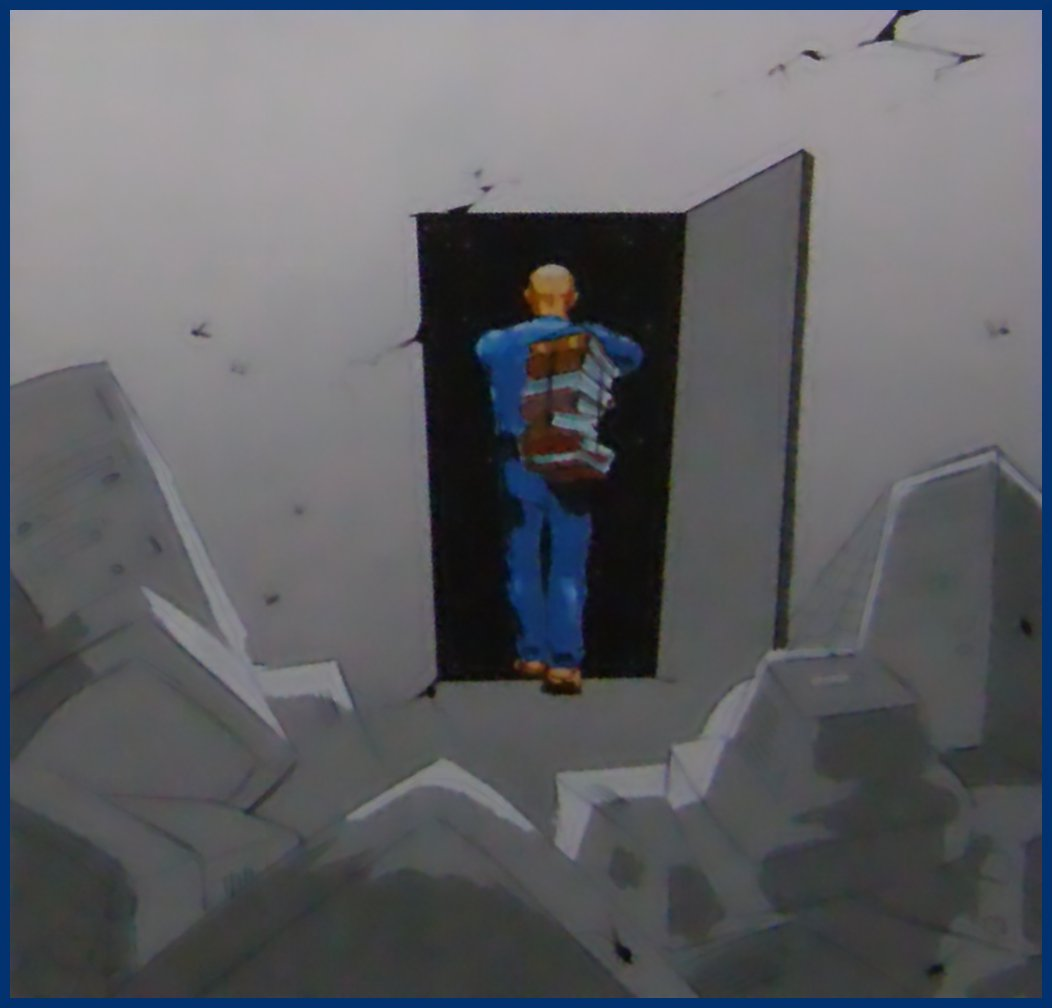
\includegraphics[width=#1\textwidth]{cover.jpg}}
\newcommand{\firstcoverline}[1]{ {\noindent \fontsize{#1}{#1}\selectfont\textbf{Вселенная}} }
\newcommand{\secondcoverline}[1]{ {\noindent \fontsize{#1}{#1}\selectfont\textbf{Александра Казакова}} }

\extratitle{
\vfill
\switch
\case{\isAFour}
	\firstcoverline{36pt}
	\vskip 0.5\baselineskip
	\secondcoverline{36pt}
	\vskip 2\baselineskip
\case{\isIPad}
	\firstcoverline{36pt}
	\vskip 0.5\baselineskip
	\secondcoverline{36pt}
	\vskip 2\baselineskip
\case{\isSevenInches}
	\firstcoverline{18pt}\secondcoverline{18pt}
	\vskip 0.5\baselineskip
\endswitch
\coverimage{1}
}

% title
\date{}
\title{Вселенная Александра Казакова}
\subtitle{и Клуб Александра Казакова}
\date{}
\publishers{\small{Собрано и сверстано Богданом Опанчуком, \\ скомпилировано \today \\ Мельбурн, Австралия}}

\maketitle

\frontmatter

\clearpage
\begingroup
	% Disable page numbers for ToC and foreword
	\pagestyle{empty}
	\renewcommand*{\chapterpagestyle}{empty}
	\tocloftpagestyle{empty} % due to tocloft package, ToC is not affected by common page style

	\renewcommand{\@pnumwidth}{\tocnumwidth}
	\renewcommand{\@tocrmarg}{\tocmarginwidth plus1fil} % make ToC flushed to the left

	\begin{spacing}{\tocspacing}
	\tableofcontents
	\end{spacing}

	\addchap*{От составителя}

В конце 90-х и начале 2000-х годов в России выходил журнал под названием {\flqq}Подводная лодка{\frqq}, позже переименованный в {\flqq}ПЛ: Компьютеры{\frqq}. И работал в этом журнале главный редактор Петр Курков, писавший иногда под псевдонимом Александр Казаков. Однажды он, по всей видимости, решил, что чужих колонок ему мало и основал свою персональную Вселенную в рамках одного журнала.

Так и появилась {\flqq}Вселенная Александра Казакова{\frqq}, пристанище для эссе на социальную, компьютерную и вообще всякую тематику. Через некоторое время начал писать эссе под собственным именем, но дух Казакова иногда возвращался, чтобы помочь своему создателю с очередным произведением. Так бы и осталась вся эта Вселенная творением одного человека, если бы один раз в порядке исключения к ее наполнению не приложил руку другой главред ПЛ{\mdash}Генри Шеппард. Через несколько лет колонка сколлапсировала, а еще через некоторое время перестал выходить и сам журнал.

Я читал ПЛ, когда он еще выходил, и покупал его во многом из-за казаковских эссе. К счастью, еще до того как сайт журнала растворился в интернете, я успел выкачать все доступное содержимое колонки. Сейчас в поисковиках можно найти лишь небольшую его часть, поэтому я решил немного исправить ситуацию. Эти эссе заметно повлияли на мое мировоззрение, и я считаю, что они достойны {\flqq}послежизни{\frqq}.

К сожалению, эта компиляция неполна. Часть эссе из середины пропущена, и я сумел найти только два журнала с {\flqq}Клубом Александра Казакова{\frqq}{\mdash}идейным последователем Вселенной. Кроме того, в свое время все даты публикаций я посчитал несущественными и не сохранил их (поэтому эссе расположены \emph{почти} в порядке публикации). А еще первое эссе было представлено на сайте как пять отдельных, причем в перепутанном порядке; надеюсь, мне удалось правильно его восстановить. Наконец, как мне кажется, часть названий тоже неполна{\mdash}почти везде автор придерживается паттерна с двойными названиями, но кое-где это правило не соблюдается. 

Если у вас есть какая-либо отсутствующая здесь информация, или исправление существующей, пишите мне на адрес, указанный в подписи. Также весьма приветствуются замечания об опечатках и огрехах верстки.

\nopagebreak
Приятного чтения!

\nopagebreak
\singlespacing

\nopagebreak
\hfill \textit{Богдан}

\nopagebreak
\hfill \url{bogdan@vladimirsson.info}

\clearpage
\endgroup


% ======================================================================
% Essays
% ======================================================================

\mainmatter

\addpart{Вселенная Александра Казакова}

\essay{Об интеллектуальной честности дилетантства}{Об интеллектуальной честности...}{\authorak}

\myepigraph{...Высшее образованье{\mdash}\\ Доскональное знанье \\ Вещей, невозможных никак!}
{Редьярд Киплинг}

Постоянные читатели предыдущей версии {\flqq}Подводной лодки{\frqq} могли неоднократно наблюдать на ее страницах высказывания автора этих строк по самым разным поводам. Тем, кто эти высказывания еще и читал, должно быть известно: заниженной самооценкой автор не страдает. Однако до мании величия дело тоже еще не дошло (надеюсь).
Так что поверьте: появление персональной казаковской вселенной{\mdash}не его инициатива. Автор очень долго не мог понять даже, в каком свете рассматривать это мироздание; поэтому первый день творения с его сакраментальным {\flqq}Да будет Свет{\frqq} все медлил и медлил с наступлением... В конце концов (вернее, в Начале Начал), было решено творить мир от противного. От самого противного, что только можно найти. А самым противным для автора (потому что до отвращения навязло в зубах) является понятие {\flqq}информационная вселенная{\frqq}. Поэтому вселенной Александра Казакова просто доктор прописал стать принципиально дилетантской. И это{\mdash}не только стремление повыпендриваться.

Вообще говоря, у человека есть три пути познания мира. Первый{\mdash}умственный (рассуждение, анализ, выводы); второй{\mdash}поглотительный (получение внешней информации путем чтения, наблюдения и~т.~д.); третий{\mdash}непосредственное откровение Свыше. Последний путь мы здесь рассматривать не будем, т. к. в наше время не только избранных, но уже и званых-то почти не осталось, одни самозванцы; поэтому половина человечества путает откровение с белой горячкой, а вторая находится с откровениями на такой короткой ноге, что без особого повеления собственных карманных Высших Сил сморкнуться не может. Впрочем, к Высшим Силам мы еще вернемся.

Первый, умозрительно-логический путь заложил базу нашей культуры. Да и впоследствии именно по нему шли философы, пытаясь чистым рассуждением проникнуть в области, опыту недоступные. Второй путь, информационно-потребительский, в чистом виде очень хорош для уяснения: из опыта{\mdash}простых бытовых истин ({\flqq}Туча{\mdash}к дождю{\frqq}; {\flqq}Нашел миллион{\mdash}богатым будешь{\frqq} и~т.~д.), из книжек и газет{\mdash}простых фактов окружающего мира. Сочетание первого и второго путей порождает опытово-научный подход (рассуждение на базе информации с постоянной проверкой результатов). Все это было бы очень гармонично, но, к сожалению, в нашем {\flqq}информационном обществе{\frqq} второй способ познания распух и задавил первый. Массы людей перестают думать, как только научатся читать. Среди них затем выделяются начитавшиеся до упора экземпляры, которые начинают еще и писать. Тьма экспертов, специалистов и профессионалов вываливает на человека чудовищные груды информации, приправленные{\mdash}для виду{\mdash}имитацией рассуждения. Имитацией, потому что корректность подбора исходной информации{\mdash}на совести {\flqq}вываливающего{\frqq}. {\flqq}Владеющий информацией эксперт{\frqq} может из всего множества фактов подобрать такие, которые заведомо ложатся в рамки его теории; он может так манипулировать этой информацией, что из чего угодно выведет что угодно. Рассуждение здесь играет абсолютно декоративную роль{\mdash}ведь читатель не может поймать эксперта за руку в фактологической области.

Таким образом, попытка противопоставить всему этому {\flqq}информационному буму{\frqq} голос воинствующего дилетанта{\mdash}не наглость, а всего лишь плод интеллектуальной честности. В этой вселенной вам не будут давить на психику ссылками и фактами (половину из которых невозможно проверить, а вторая половина трактуется {\flqq}профессионалом{\frqq} вполне произвольно по тому же праву {\flqq}владения информацией{\frqq}). Автор собирается ходить исключительно первым путем{\mdash}то есть рассуждать и умствовать. Поэтому и читателю не придется ничего принимать на веру: все авторские тезисы всегда можно будет проверить на вшивость, владея лишь рассудком и умом...

Разумеется, автор также оставляет за собою право по ходу дела стебаться, проводить безответственные аналогии и вообще мухлевать забавы ради. Но все это{\mdash}в той же области логических (то есть в данном случае{\mdash}псевдологических) рассуждений. А уж где розыгрыш, а где серьезный тезис{\mdash}вычислять вам. На то и мозги, не так ли?

\essaysection{Для простоты примем {\flqq}пи{\frqq} равное трем...}

\myepigraph{...Первичная цель состоит в выявлении аналогий, а уж вторичная{\mdash}в поиске объяснений. \\
...Найденные объяснения по определению являются научными.}
{Умберто Эко}

Говорят, именно так начинался один из любительских трактатов по вычислению квадратуры круга. В результате эта самая квадратура была в нем исчислена совершенно верно и очень быстро. Достаточно было одного маленького начального допущения...

Подобные подстановки очень характерны для новейших мифов, тщащихся (эх, какое слово-то богатое!) стать Истинами. Внешне механизмы подтасовки весьма разнообразны, но на деле сводятся к одной базовой операции: чтобы впарить доверчивому читателю, что из имеющегося X следует желанное Z, это самое X неявным образом (по умолчанию, или запутав, или запугав читателя) элегантно превращают в некоторое Y, действительно с искомым Z связанное. Каковой факт впоследствии и доказывают вполне честно. Главное{\mdash}в эпилоге не забыть обратно превратить Y в X. Але-ап!{\mdash}и из любой шляпы вынимается любой кролик.

Автором обнаружено 4 основных метода выполнения этой операции:

1) Непосредственная подтасовка исходной информации, выдумывание или искажение фактов. По этой, самой грубой, схеме построены все уфологические и половина экологических мифов. Уфологи (пророки НЛО) вообще процветают лишь за счет вопиющего невежества читающей {\flqq}образованной{\frqq} публики в области астрономии и физики. Но ниже мы специально не будем заострять внимание на этом методе{\mdash}ведь у нас принципиально дилетантская вселенная, верно? Значит, в справочники и первоисточники мы лазить не станем. Изящнее и элегантнее сыграть с пророком-экспертом на его поле, т.~е. принять все предложенные им посылки, а затем все равно поймать его с поличным.

2) Аналогическое запутывание, или вакханалия взаимосвязей. При этой методике на читателя вываливается ворох аналогий и надуманных связей между явлением X и явлением Y, и уравнение X=Y считается доказанным тем вернее, чем больше этих аналогий и связей высосано из пальца (например: {\flqq}У человека, как и у циркуля, две ноги. Некоторых людей называют {\glqq}железными{\grqq}{\mdash}но ведь и циркуль железный. Циркуль предназначен для рисования кругов{\mdash}но нам хорошо известно выражение {\glqq}ходить по кругу{\grqq}... следовательно, некоторые люди{\mdash}инкарнации циркулей{\frqq}). При этом главное{\mdash}привести как можно больше аналогий, пусть даже самых натянутых и бессистемных, не давая читателю передохнуть (Кто говорил: {\flqq}Врите как можно больше, что-нибудь да останется{\frqq}{\mdash}Талейран или Геббельс?), и не упоминать о незначительных и второстепенных различиях между человеком и циркулем.

По терминологии, предложенной одним из героев {\flqq}Маятника Фуко{\frqq} Умберто Эко, любители этого метода{\mdash}{\flqq}дураки{\frqq}. {\flqq}Дурак начинает с того, что собака домашнее животное и лает, и приходит к заключению, что коты тоже лают потому, что коты домашние... Дураки публикуются легко, потому что с первого наскока выглядят убедительно{\frqq}. Но мы вынуждены с мэтром не согласиться. Это обычно как раз достаточно умные люди, которые просто пытаются нас с вами оставить в дураках...

3) Агрессивная псевдологика. Самый простой и самый незаметный метод. Если связь некоего фактика X' с фактиком Y' на самом-то деле всего лишь возможна или хотя бы не исключена, искусный мифотворец построит фразу так, что наличие этой связи станет выглядеть абсолютно доказанным фактом. Если явление X' можно объяснить через Y', то именно это объяснение будет преподнесено как единственное. На самом деле никаких доказательств вам не приведут, но вам покажется, что они были. Некоторые умельцы минируют таким образом почти каждую свою фразу. Для маскировки здесь используются обычно литературные приемы{\mdash}интонация, ирония, риторика и эмоционально-доверительный фон, поэтому широко применять псевдологику рискуют только хорошие стилисты.

4) Последний из основных методов{\mdash}уже упоминавшийся терминологический террор. Его суть проста. Явление X начинает описываться в терминах, используемых для описания явлений типа Y... и, собственно, все. Больше ничего не надо. Если вы никогда не задумывались над тем, что наше восприятие явления полностью зависит от терминологической среды, в которой оно описано, вспомните хотя бы знаменитый перевод {\flqq}инструкции к мыши Windows{\frqq} с помощью автопереводчика со встроенным медицинским словарем. Характерный пример терминологического террора мы приведем ниже, когда начнем разбираться с некоторыми компьютерными мифами (А вы уже и не надеялись, что это эссе будет хоть как-то соприкасаться с тематикой журнала? Успокойтесь, немножечко будет. Но только для маскировки...).

Упоминая своих критиков, хороший мифотворец использует два дополнительных приема. Во-первых, он сразу вешает на них какой-нибудь ярлык; в этом сезоне наряду с классическими {\flqq}ретроградами{\frqq} очень хорошо идут {\flqq}так называемые марксистские... (далее по ситуации){\frqq}. Во-вторых, он с бесконечным терпением и состраданием на паре страниц заливается соловьем, что понимает, как это тяжело, когда приходится ломать стереотипы... как многие не выдерживают... как они его, бедного, ругательски ругают, но он все стерпит ради победы Истины... Далее приводится парочка выдранных с мясом критических цитат (действительно, как правило, содержащих нелицеприятные выводы; например, из нашего эссе любой мифотворец с радостью процитирует абзац про дураков{\mdash}для того и вставлено...){\mdash}и дело в шляпе. Любая критика поборника Истины отныне воспринимается предвзято, подсознательно ассоциируясь с моветоном.

Чтобы вся эта сухая теория слегка озеленилась, приложим ее к некоторым клюквенным лесопосадкам нашего времени (Вот тоже фразочка{\mdash}специально для цитирования обиженным пророком! Дарю!).

\essaysection{Квадратно-гнездовой способ мышления}

\myepigraph{Механизм нынешнего языка сберегает умственный труд куда больше, чем следует. Длинные слова дребезжат, словно длинные поезда. Они везут сотни людей, которые слишком бездумны, чтобы думать самостоятельно.}
{Гилберт К. Честертон}

К сожалению, вышеупомянутое {\flqq}владение рассудком и умом{\frqq} ныне не так модно, как {\flqq}владение информацией{\frqq}. В любой голове (не исключая и авторскую) имеются слепые пятна, плохо пригнанные детальки, несцепляющиеся шестеренки. Аналогия с механизмом, конечно, неверна: мыслительный аппарат разбалтывается не от частого употребления, а от пренебрежения. Чем больший объем информации некритически усваивается человеком, тем больше в его сознании дыр, тем слабее его иммунитет к следующей порции бездумно воспринимаемых {\flqq}вводных{\frqq}... И так{\mdash}вплоть до полной шаблонности, когда мышление заменяется симпатичным протезом наподобие органчика из головы одного из Глуповских градоначальников...

Нет, автор не пытается эпатировать общественность (ну-у... почти). Однажды им уже было отмечено, что стандартный тип мышления вообще {\flqq}напоминает складывание паззла: в мозгу перемещаются и притираются друг к другу базовые блоки, типовые истины. Получившиеся умозаключения состоят из того или иного набора этих мысле-атомов; внутрь самих блоков сознание мыслителя проникнуть не может. Для него они являются аксиомами, неделимыми частичками мышления...{\frqq} Такие блоки могут быть самых разных размеров. Для многих это{\mdash}целиковые суждения, кем-то когда-то высказанные, а теперь принятые на веру, как нечто, не подлежащее препарированию и анализу (типа {\flqq}все мужчины сволочи{\frqq}, {\flqq}смертная казнь{\mdash}нарушение прав человека{\frqq}, {\flqq}жиры вредны для сердца{\frqq}). Для других{\mdash}это слова и словосочетания, которым заведомо приписан какой-то определенный смысл. Только немногие умеют вскрывать еще и внутреннее строение самих словоформ и обнаруживать, что и они состоят из понятий, а каждая данная комбинация этих понятий не всегда так уж бесспорна...

Естественно, чем мельче мысле-атомы{\mdash}тем их больше, тем больше их комбинаций, тем совершеннее мышление. Менее очевиден другой факт: весь наш нынешний информационный бум приводит вовсе не к размельчению мысле-атомов, а к их укрупнению и укреплению. Дело в том, что со скоростью инфузорий размножаются вовсе не оригинальные понятия, а различные тезисы, термины и словосочетания; но каждый такой ублюдок, становясь в чьем-то сознании мысле-атомом, поглощает входящие в него понятия, выводя их из сферы рассудка.

Поясним на паре примеров. Последнее время в различных интервью, посвященных личной жизни богемы, постоянно проскальзывает клише типа {\flqq}X и Y живут в гражданском браке, но вскоре собираются расписаться и обвенчаться{\frqq}. Автору совершенно до лампочки, как и с кем кто живет, но {\flqq}гражданский брак{\frqq} по определению как раз предполагает, что люди уже расписались в ЗАГСе (отделе Записи Актов Гражданского Состояния, если кто не в курсе). И названа так эта форма брака была в XIX в., чтобы отличить ее от полноценного{\mdash}по тогдашним понятиям{\mdash}{\flqq}церковного брака{\frqq}. А наши уважаемые X и Y на самом деле {\flqq}сожительствуют{\frqq}. Однако это слово кажется каким-то... унизительным, верно? Что же, тем хуже для слова. А заодно и для понятия. Теперь это тоже будет называться {\flqq}гражданским супружеством{\frqq}, а понятие {\flqq}сожительства{\frqq} мы оставим исключительно для бомжей. А раз нет больше (по крайней мере, в {\flqq}высших сферах{\frqq}) такого слова{\mdash}значит, никто и подумать соответствующим образом не сможет...

Или возьмем замечательный AI, которым так любят хвастаться создатели компьютерных игр и который так любят ругать игровые журналисты. Гордое словосочетание {\flqq}искусственный интеллект{\frqq} в реальности означает более-менее подробное дерево решений, заранее прописанное программистом. Совершенно по такому же принципу реагируют на окружающий мир насекомые, только у них это{\mdash}от природы. Выходит, таракан теперь обладает {\flqq}естественным интеллектом{\frqq}, что ли? Но если {\flqq}интеллект{\frqq}{\mdash}нечто, что есть и у меня, и у Windows'98, и у таракана, и у игрового монстра, то это понятие становится слишком широким. Мысле-атом разбухает и поглощает окрестные оттенки смысла.
В качестве упражнения предлагаю читателю самостоятельно попробовать вскрыть мысле-атомы {\flqq}демократические реформы{\frqq} и {\flqq}компьютерная грамотность{\frqq}, чтобы вернуть в личное обращение понятия, с недавних пор заключенные в темницу этих штампов.

Братья Стругацкие в {\flqq}Пикнике на обочине{\frqq} полусерьезно выдвинули пессимистическую теорию: разум{\mdash}это всего-навсего сложный процесс формирования у одного вида обезьян неких новых инстинктов. Пока идет это становление{\mdash}все кипит и перемешивается, но закончится процесс, как обычно, кристаллизацией одного огромного моноблока, внутри которого движение мысли застынет... Картина жутковатая, но в нее вполне вписывается наблюдаемая тенденция{\mdash}Слово, которое на заре разума было его основой и двигателем, ныне становится шаблоном, песком в шестеренках сознания...

Но ползучий рост мысле-атомов{\mdash}только один из тараканов, которых {\flqq}информационное общество{\frqq} усердно разводит в наших головах. Очень часто человек, проникшийся какой-нибудь концепцией, возводит ее целиком в ранг центрового личного мысле-атома. Этот огромный, непроницаемый кирпич ложится в середину сознания, и траектории всех прочих блоков отныне должны его огибать и к нему приспосабливаться. Называется кирпич обычно {\flqq}позицией{\frqq}, {\flqq}мировоззренческим фундаментом{\frqq} или {\flqq}точкой зрения{\frqq}. И все бы неплохо, человека без точки зрения тоже особо мыслящим не назовешь. Но дело-то в том, что фундаменты, доставшиеся нам в наследство от прежних веков, шлифовались и доказывались столетиями, пройдя в том числе проверку логикой и рассуждениями. Мысле-атомами они не являются: каждый может проникнуть внутрь и подергать за связки, убедившись в прочности конструкции. Люди, выбравшие тот или иной из подобных фундаментов, попросту не стали изобретать велосипед (хотя вполне способны его разобрать и собрать заново). А вот {\flqq}информационная революция{\frqq} подарила нам огромное множество {\flqq}позиций{\frqq}, основанных исключительно на манипуляции огромными грудами фактов (или измышлений, выдаваемых за факты) или вообще на {\flqq}терминологическом терроре{\frqq}, когда ученость слога автоматически подразумевает непогрешимость автора. А ведь обычный современный человек доверчив и в концептуальном плане напоминает свежевылупившегося цыпленка, который, как известно, первый же увиденный движущийся предмет отныне считает мамой; современный человек первую же встречную {\flqq}консепсю{\frqq} примет за символ веры{\mdash}и получит огромный камень в стеклянный дворец своего рассудка.

При этом куча {\flqq}новых мировоззрений{\frqq} благополучно погребла под собою старинные фундаменты, задавив их количеством. Лист легче всего спрятать в лесу, песчинку{\mdash}на пляже; вечные и разумные истины надежно спрятаны от нас в завалах {\flqq}истин{\frqq} юных, агрессивных и требующих не познания, а признания.

Изучим внутреннее строение таких конструкций со специальной целью: понять, как им удается прикинуться убедительными.

\essaysection{Самое прибыльное историческое обрезание}

\myepigraph{{\sdash} Я{\mdash}историк,{\commamdash}подтвердил ученый и добавил ни к селу ни к городу: \\
{\sdash} Сегодня вечером на Патриарших прудах будет интересная история!}
{Михаил Булгаков}

Может быть, на Патриарших прудах история и была, зато нам точно известно, что на Воробьевых горах она недавно быть перестала. Профессор математики, на досуге создававший весьма талантливые гравюры апокалиптического содержания, обратил свое внимание на историю и решил, что из нее тоже можно нарезать неплохой Апокалипсис. Только наоборот: ангелы из откровения Иоанна Богослова уверяли, что однажды {\flqq}времени больше не будет{\frqq}, а профессор популярно объяснил, что времени никакого и не было... Обрезание истории, видимо, оказалось занятием куда более благодарным, чем вырезание по дереву: сторублевые фолианты самого профессора и его последователей блистают в книжных магазинах золотым тиснением, напрочь затмив невзрачные и скучные книжонки {\flqq}ортодоксов{\frqq}...

Речь идет о {\flqq}новой хронологии{\frqq}, предложенной А.Т. Фоменко и его последователями. Мы настоятельно советуем читателю в целях тренировки иммунитета изучить пару-другую соответствующих текстов. Будем справедливы: пассажи типа {\flqq}я этого Фоменку не читал, но категорически с ним не согласен{\frqq} выглядят несколько неспортивно.

Вкратце напомним сюжетную линию сенсации. Изучив {\flqq}Альмагест{\frqq}{\mdash}звездный каталог якобы Птолемея, датированный II в н. э.,{\commamdash}американский астроном Р. Ньютон объявил его подложным. По Ньютону, положения звезд в {\flqq}Альмагесте{\frqq} соответствуют скорее X в. Фоменко подтвердил вычисления Ньютона, но сделал из них куда более сильный вывод: Птолемей, по Фоменко, действительно жил в IX{\ndash}XIII вв., а никакого древнего мира и античности не было. Все {\flqq}античные{\frqq} документы написаны в тех же IX{\ndash}XIII вв., относятся к текущим событиям того времени и лишь впоследствии, в силу некой глобальной путаницы с хронологией, географией и именами собственными, оказались как бы {\flqq}сдвинуты{\frqq} в прошлое{\mdash}большинство на 1053 года, некоторые на 330, а какие и на все 1800 лет. Так и возник {\flqq}виртуальный древний мир{\frqq}, являющийся лишь дву- и трехкратным отражением событий средневековья... Захватывает, не правда ли?

...Историю с {\flqq}Альмагестом{\frqq} принципиально оставим в покое. Как уже отмечалось, все приводимые факты мы принципиально будем считать верными. Следовательно, мы пока согласимся считать {\flqq}Альмагест{\frqq} составленным около X в. Но что, по-вашему, естественнее: признать фальсифицированным один документ или объявить неправильно датированным огромный массив документов? Правильно. Нормальные герои всегда идут в обход.

И здесь начинается пиршество метода {\flqq}аналогического запугивания{\frqq}. Фоменко приводит огромное количество параллелей и повторов, доказывая, что известная история{\mdash}это {\flqq}склейка{\frqq} из четырех дубликатов истории реальной, начавшейся в X в. Объем информации поражает. Императоры, войны, события мельтешат в бесчисленных таблицах и графиках, танцуя странный танец отражений, и уследить за этим водоворотом очень трудно (на что, видимо, и расчет). Если Фоменко два раза обратил наше внимание на сходство имен и прозвищ, то на третий раз он без комментариев ставит рядом Суллу Люция и Оттона Лютого, и задерганное сознание всерьез воспринимает это как очередную параллель... Для полноценного разбора необходимо комментировать каждую связку, что потребует книжки раза в четыре толще оригинала. Но апофеозом аналогий является отождествление Иисуса Христа с римским папой Григорием VII. Советуем самостоятельно изучить этот душераздирающий хроноклазм (бедный папа Григорий! В каждой булле именовал себя {\flqq}наместником Христа{\frqq}{\mdash}и так и не узнал бы никогда, что был своим собственным наместником, если бы не Фоменко...) и попытаться найти в фоменковских {\flqq}аналогиях{\frqq} место для Понтия Пилата, царя Ирода и Кайафы... Маститый мифотворец не счел нужным упомянуть о таких второстепенных личностях...

А чтобы до конца разобраться с историческими параллелизмами, послушайте одну занятную историю.

...Революция в одной европейской державе смела монархию, но республика тоже долго не продержалась: к власти пришел воинственный диктатор, назвавший свою страну {\flqq}империей{\frqq} и пожелавший добиться мирового господства. Довольно быстро он подчинил себе почти всю континентальную Европу{\mdash}и началась странная война с островной Англией. Войска диктатора царили на суше, но Англия, как всегда, владычествовала морями. Диктатор понял: чтобы сокрушить Англию, надо вторгнуться в Россию, ибо только так можно проникнуть к Индии{\mdash}сердцу Британской Империи. Он дошел до Москвы, однако далее фортуна повернулась к нему спиной: то ли мороз, то ли русская доблесть вынудили его отступить. Теперь уже русские вступили в Европу, и ненадежные вассалы диктатора один за другим поворачивали оружие против него; высадились в Европе и воспрявшие духом англосаксы. В конце концов великий диктатор пал, а победители, заседавшие в древней королевской резиденции вблизи столицы бывшей империи, выработали послевоенное устройство Европы, определившее ее судьбу на последующие десятилетия. И все это{\mdash}от революции до капитуляции{\mdash}заняло 26{\ndash}27 лет...

О ком это я? О Наполеоне или о Гитлере? О Франции 1789{\ndash}1815 гг. или о Германии 1918{\ndash}1945 гг.? Ответить невозможно: все описанные события действительно произошли дважды. Мы имеем аналогию куда более полную, чем все фоменковские, и доказывает она только одно{\mdash}аналогии вообще ничего не доказывают...

Присутствует здесь и метод № 3. Для доказательства основной идеи используются взаимоисключающие тезисы, но они разнесены по тексту (или даже по книжкам разных авторов из группы Фоменко), чтобы читатель попросту успел забыть, что ему там раньше говорили. Например, в {\flqq}Лекции 1{\frqq} упомянутого реферата А. Г. Фоменко для доказательства условности древней хронологии приводит список дат {\flqq}сотворения мира{\frqq}, употреблявшихся разными хронистами и отличающихся одна от другой на сотни лет; а в {\flqq}Лекции 14{\frqq}, цитируя этих самых хронистов, подставляет в свои вычисления совершенно конкретную дату, чтобы получившимся результатом можно было умыть современных историков. Далее, в {\flqq}Лекции 11{\frqq} Вифлеемская звезда отождествляется со Сверхновой 1054 г.; вовсю используется почти абсолютное совпадение с вышеупомянутым 1053-летним сдвигом. Однако эта Сверхновая исторически известна из китайских хроник, а по мнению последователей Фоменко ({\flqq}Хронотрон{\frqq} С. Валянского и Д. Калюжного), китайская хронология достоверна вообще только с XVII в. Т. е. китайцам верить вообще-то нельзя, но если очень хочется{\mdash}то можно...

С {\flqq}открытиями{\frqq} Валянского, Калюжного (и примкнувшего к ним беллетриста Бушкова) связан еще более занятный пример метода № 3. Собственно, {\flqq}закрытие Китая{\frqq} потребовалось им в связи с основной идеей фикс{\mdash}отменой татаро-монгольского ига. По Бушкову-Валянскому-Калужному, монголо-татар никаких не было вообще. Но, поскольку чингизиды имели наглость отметиться по всему Востоку (например, основали династии в Китае и Индии){\mdash}пришлось дезавуировать 90\% восточной истории, сославшись на глобальные чистки архивов, имевшие место в Китае в XVI{\ndash}XVII вв. Отсель, якобы, и началась настоящая китайская история. Замечательно. Только беда в том, что монголы сильно наследили в историографии еще одной страны, имеющей непрерывную культурную традицию, восходящую к VIII в. Автор этих строк долго ломал голову: как же Бушков и Валянский-Калюжный будут отменять японскую историю? Но действительность оказалась радикальнее всех прогнозов. Они упразднили ее вместе с Японией. Во всем {\flqq}информационном пространстве{\frqq} этих книжек о Японии нет ни помину, ни намеку. Решение, несомненно, экономное: зачем мучиться, доказывать призрачность еще одной истории, зачем пытаться и японскую историю дезавуировать, если можно просто промолчать? Авось читатель, задавленный {\flqq}информацией{\frqq}, не заметит {\flqq}пропажи бойца{\frqq}... И действительно, тексты слеплены так плотно и экспрессивно, что дыра на месте Страны Восходящего Солнца становится почти незаметной...

{\flqq}Терминологического террора{\frqq} в сочинениях Фоменко нет. Действительно, как-то не к лицу математику пугать читателя гуманитарной терминологией{\mdash}да нас ею особо и не запугаешь, ведь большинство еще помнит суровые времена исторического материализма... А вот в родной {\flqq}Подводной лодке{\frqq} автор недавно обнаружил серию статей, {\flqq}позиция{\frqq} которых держится исключительно на методе № 4. Возможно, переход от сенсации года к внутрижурнальной полемике может показаться слишком резким{\mdash}но зато примите во внимание, что мы наконец-то поворачиваемся лицом к родной информационно-компьютерной тематике...

\ifcase\isAFour
	% for some reason TeX leaves header&epigraph at the end of the page here
	% even with \nopagebreak between epigraph and heading and nopagebreak after epigraph
	\pagebreak 
\fi

\essaysection{Протез религии, или Божки из кармана}

\myepigraph{В рецензии на книгу Гранта Аллена {\flqq}Эволюция идеи Бога{\frqq} я заметил, что интереснее было бы прочитать Божью книгу {\flqq}Эволюция идеи Гранта Аллена{\frqq}...}
{Гилберт К. Честертон}

Постоянные читатели {\flqq}ПЛ{\frqq}, наверное, обратили внимание на опубликованный в №№ 7{\ndash}9 триптих Г. Далидовича {\flqq}Машина как средство познания себя{\frqq}. Выступая в качестве продвинутого компьютерного пророка, автор сериала проходится по всем аспектам человеческого мышления и доказывает их полное тождество с соответствующими функциями Машины (т.~е. компьютера). Любопытно простодушное объяснение автора, почему для описания человеческой психики он выбрал компьютерную терминологию. {\flqq}Встал вопрос: какую базовую терминологию при этом использовать? Выдумывать свою{\mdash}засорять информационное пространство. Использовать какую-либо из общепринятых{\mdash}негласно примкнуть к одной из школ. А каждая из них тенденциозна по-своему{\frqq}... Как видим, основной принцип {\flqq}терминологического террора{\frqq} Г. Далидовичу хорошо известен{\mdash}способ описания существенно влияет на представление об описываемом. {\flqq}Как вы лодку назовете, так она и поплывет...{\frqq} Однако сам он, не колеблясь, излагает свою теорию о {\flqq}механизмах мозга{\frqq} в терминах процессоров, ОС, быстродействия и многозадачности... Разумеется, он тут же получает желаемый результат, потому что этот результат уже жестко заложен в сам способ изложения проблемы. Когда средневековый философ начинал анализировать те же проблемы мышления в богословских терминах{\mdash}его выводы тоже были предопределены, но этого монаха мы почему-то именуем {\flqq}схоластом{\frqq}, а современного компьютерщика-эзотериста величаем {\flqq}мыслителем{\frqq}...

Но интереснее всего другой аспект трилогии Г. Далидовича, который сближает его {\flqq}позицию{\frqq} с бесчисленным легионом прочих модных {\flqq}концепций{\frqq} нашего времени. Далидович пишет о чудовищном потоке эзотерических учений, заполонившем нашу культуру, и свою работу он скромно рассматривает как попытку навести во всем этом порядок {\flqq}с точки зрения информационных взаимодействий{\frqq}. Причем сам он, несмотря на ультратехнократическую терминологию, тоже материалистом не является: на заднем плане его концепции постоянно маячит некий {\flqq}Администратор Сети{\frqq}, который однажды извлечет наш {\flqq}самообучающийся программный модуль из устаревшего изношенного железа. Извлечет его без ненужной личностной памяти и определит его ценность... В зависимости от текущих задач и ценности Модуля он будет либо уничтожен, либо направлен на выполнение новой задачи... Вот и все. Очень просто. Все религии говорят о том же самом, но в ограниченном понимании своих интерпретаторов{\frqq}...

Во-первых, чувствуете ли вы знакомый запах избранничества, всегда окружающий нынешних эзотериков? Все прежние религии были ограничены, все они говорили об одном и том же, только не могли этого понять; но МЫ-то знаем... Позвольте по этому поводу привести встречную цитату из того же Умберто Эко{\mdash}лучше него все равно не скажешь. {\flqq}Синкретизм{\mdash}это не просто сочетание разноформных верований и практик. Здесь основа сочетаемости{\mdash}пренебрежение к противоречиям. Исходя из подобной логики, все первородные откровения содержат зародыш истины, а если они несовместимы, это не имеет значения... Из этого вытекает, что нет места развитию знания. Сам по себе принцип валить в кучу Августина и Стоунхедж{\mdash}это и есть симптом Вечного фашизма{\frqq}.

Разумеется, обвинять Г. Далидовича и прочих честных эзотериков, имя которым легион, в осознанном интеллектуальном фашизме{\mdash}несправедливо. Это просто люди, которые застряли в трясине, лежащей между религией и атеизмом. Что-то высшее в мироздании им иметь хочется; они нутром чуют, что это даст картине мира необходимую завершенность. Но при этом веру в конкретного, личностного, определенного и грозного Бога монотеистов они считают устаревшей, слишком жесткой, ограничивающей их умственную свободу. И вот так на свет появляются сонмы частных, личных божеств{\mdash}{\flqq}Администратор Сети{\frqq}, {\flqq}Мировой Дух{\frqq}, {\flqq}Космическая Энергия{\frqq}, {\flqq}Абсолют{\frqq} и~т.~д., и~т.~п. Эти зыбкие, бесформенные божки очень удобны: они легко подгоняются по форме жилетного кармана. Нынешние пророки свободно творят себе богов по потребности, и в этом смысле они действительно свободны.

Но такая {\flqq}интеллектуальная свобода{\frqq} означает всего-навсего отказ от интеллектуальной честности. Действительно, при ближайшем рассмотрении ясно, что честны только две мировоззренческие позиции: атеиста и монотеиста. Атеист последователен: он знает, что Бога нет, что ничего, кроме природы и ее законов, на свете нет{\mdash}и эта позиция неуязвима. Монотеист, принимая Бога, Творца всего сущего, честно признает за ним все его атрибуты наподобие всемогущества, внеприродности, личностности. Но ущербные, неопределенные божки нового времени{\mdash}это ни рыба ни мясо. В материалистическую Вселенную они не лезут, потому что являются элементом мистическим и сверхъестественным. Но кинопробу на роль Творца в идеалистической Вселенной они тоже благополучно проваливают, т. к. безлики, неконкретны, безличны; их никак не назовешь {\flqq}Высшей Силой, Полнотой Всезнанья и Первою Любовью{\frqq}. Единственное, что им остается{\mdash}функция личных божков наподобие деревянного Мумбо-Юмбо какого-нибудь папуаса. Действительно, ведь они вторичны: их строгают из полена с целью подогнать под какую-нибудь уже готовую идею и тем самым задним числом эту идею освятить.

...Одна моя знакомая, полагающая себя католичкой, на исповеди не считала нужным каяться в прелюбодеяниях, потому что соответствующую заповедь трактовала по-своему: если, мол, люди нравятся друг другу, то это уже не прелюбодеяние. Таким образом, она создала себе личную редакцию заповедей, а заодно и небольшое личное {\flqq}католичество{\frqq} на одну персону. Собственно, все нынешние мыслители занимаются тем же, только с гораздо более умным видом.

В результате получается, что они ставят на место традиционного Бога некую постороннюю сущность, традиционным Богом не являющуюся; поклоняются какой-то сущности, не являющейся Богом. С точки зрения атеиста, это безразлично; но с другой точки зрения это попросту опасно...

\essay{Дорога в будущее для всадников без головы}{Дорога в будущее...}{\authorak}

\essaysection{Карманная теодицея}

\myepigraph{Если обходиться с каждым по заслугам, кто уйдет от порки?}
{Вильям Шекспир}

Если Бог{\mdash}абсолютное Добро, тогда почему Вселенная так зла? Этот якобы каверзный вопрос сильно отталкивает от веры нынешних интеллектуалов, знакомых с вопросами религии по рецензиям в глянцевых журналах и по листовкам разных {\flqq}Одноклассников Иисуса{\frqq}. Разумеется, внутри богословия есть целая отрасль мысли под названием {\flqq}теодицея{\frqq}, тысячу лет изучающая проблему мирового зла; но образованному человеку XX в. всей этой замшелости не надобно. Он предпочитает кормиться даосистско-хаббардовским мозговым компостом... Но ни в классическом богословии, ни в модернистских комиксах духовного содержания не рассматривается такой вот оригинальный вариант: что, если добрый вообще-то творец создал Вселенную из-под палки? То есть не по своей доброй (в обеих смыслах) воле? Разумеется, предположить такое о процессе творения реальной физической Вселенной может только крайне болезненный манихей; но всем, кому во {\flqq}вселенной Александра Казакова{\frqq} неуютно из-за ее недружественности, стоит помнить об этой возможности{\mdash}и не судить строго...

Отмазавшись таким образом от всех возможных нынешних и будущих обвинений в злобствовании, ерничании и предвзятости, автор с легким сердцем приступит к своим непосредственным обязанностям: со вкусом, во всех подробностях описывать те грабли, по которым ежедневно шествует уважаемая аудитория... Кстати, может, данная {\flqq}вселенная{\frqq} еще и поэтому кажется преисполненной зла? Говорить о граблях{\mdash}моветон. Грабли никак не вписываются в реальность, которую нам положено видеть по мнению поборников Гуманизма, Прогресса и Прав Человека. Нынче процесс, при котором ты на что-то наступаешь, что-то поднимается и вышибает у тебя искры из глаз, должно именовать {\flqq}движением каждого к информационному росту и видению новых перспектив{\frqq}. А тут сразу{\mdash}грабли... Народ не поймет. Нынче ведь в развитии народа наступил новый этап. Это раньше бытовали выражения типа {\flqq}пока жареный петух в темечко не клюнул{\frqq} или {\flqq}гром не грянет{\mdash}мужик не перекрестится{\frqq}. А нынче у нас информационное общество. Т. е. и гром, и жареного петуха упаковали в такую подарочную обертку из розовых слов и понятий, что сам факт клевания мужик обязан воспринимать радостно, мало того{\mdash}он сам должен искать себе означенного петуха и заблаговременно брить и мыть темечко. Иначе, пугают апологеты Прогресса, он, петух, еще и клевать не станет... и останешься ты, мужик, неклюнутый на обочине информационной магистрали...

Впрочем, достаточно уже оправдывать вселенское зло местного розлива. Перейдем ближе к темечку. В прошлом номере {\flqq}ПЛ{\frqq} автор, если помните, рассматривал основные способы создания модных {\flqq}мировоззрений{\frqq} и прочих Откровений. Было обнаружено четыре основных метода, с помощью которых новейшие пророки могут доказать запуганному обывателю все, что угодно. Затем следовали примеры. Но в той статье речь шла в основном об {\flqq}информационных подменах{\frqq}{\mdash}о способах, с помощью которых можно неявно менять смысл, предмет слова, словосочетания или фразы. С помощью таких подмен доказываются {\flqq}истины{\frqq}, являющиеся информационными же подкидышами. Одним словом{\mdash}лживые. Однако благоденствуют и такие {\flqq}мировоззренческие мышеловки{\frqq}, суть которых в этических, эмоциональных подменах. Лжи, как искажения реальности, в них нет, ловушка здесь в том, что человека заставляют радостно и с песней принять то, от чего при здравом размышлении он бежал бы с диким визгом. Или, наоборот, выставляют чудовищным (а чаще всего{\mdash}немодным и устаревшим... это самый убойный в нашем веке ярлык-киллер) что-то здоровое и естественное. К примеру, если в каком-то трактате вам доказывают, что женщина{\mdash}это биоробот, созданный пришельцами с Омеги Пеликана, а люди раньше размножались почкованием, то перед нами Откровение первого рода. А если другой Учитель вещает, что женщина{\mdash}это грязное зло, какового все честные люди должны гнушаться, и почкование{\mdash}единственный прогрессивный и гуманный способ размножения, то мы имеем дело с Откровением второго рода.

Соответственно инструментом такого Откровения является искажение не информационной, а эмоционально-экспрессивной сути слов. Его создатель не лжет{\mdash}он просто очень хитро формулирует...

\essaysection{Убили негра, убили негра...}

\myepigraph{Особая функция некоторых новоязовских слов состояла не только в том, чтобы выражать значения, сколько в том, чтобы их уничтожать.}
{Джордж Оруэлл}

Адепт того новояза, к созданию которого привела {\flqq}информационная революция{\frqq}, всегда помнит: люди в массе мыслят квадратно-гнездовым способом. Иначе говоря, они перебирают слова и словосочетания, не подвергая их внутреннему анализу. Каждое слово{\mdash}это чемодан с каким-то содержимым; но обыденное мышление манипулирует этими чемоданами, как цельными кирпичиками. Достаточно заменить содержимое{\mdash}и дело в шляпе, мозги подмены не заметят. Как это делается, мы уже видели в прошлом номере. Но давайте повторим урок, имея в виду, что вместе с содержательными подменами меняется и эмоциональная окраска.

Вот, к примеру, замечательное слово {\flqq}менеджер{\frqq}. Что оно, по-вашему, означает? Большинству из нас смутно кажется, что это название какой-то профессии. Однако если нас заставить эту профессию определить, мы начнем беспомощно разевать рот и подергивать пальцами. Действительно: дама, продающая нам двести грамм колбасы{\mdash}это продавец. Но дама, продающая нам семь дней в Анталье, уже менеджер. Может, колбаса с менеджером несовместима? Нет, ведь человек, продающий пять тонн колбасы, тоже менеджер! Мало того, девушка, не продающая ничего, но следящая, чтобы у сотрудников были ластики, а сами сотрудники пили бы кофе по графику,{\commamdash}еще один менеджер...

Фокус прост. {\flqq}Менеджер{\frqq}{\mdash}название не профессии и не должности, это неявное название некоторой социальной группы. Это ярлык для сословия людей, социальный статус которых лежит ниже {\flqq}бизнесмена{\frqq}, но уже делает для них неприличными занятия {\flqq}черным трудом{\frqq}. Иными словами{\mdash}это титул! Наподобие английского {\flqq}сквайра{\frqq}, лежащего между {\flqq}лордом{\frqq} и {\flqq}фермером{\frqq}. Любое объявление {\flqq}требуется менеджер по бармалению{\frqq} в действительности семантически означает {\flqq}на ставку бармалея приглашается джентльмен (леди) с приличными манерами и образованием{\frqq}. Но {\flqq}демократический{\frqq} характер нашего общества, параноидальная борьба с призраком дискриминации заставляют целое сословие маскироваться. Пока всем кажется, что {\flqq}менеджер{\frqq}{\mdash}профессия, никто не обвинит в дискриминации по сословному принципу предпринимателя, желающего предложить бедному, но приличному джентльмену работу, соответствующую его положению в обществе...

Или вот, скажем, {\flqq}негр{\frqq}. Что, не будем так говорить? А почему? Ах, это слово{\mdash}неприличное, уничижительное и оскорбительное... Простите, с какого перепугу оно вдруг таким стало? Всю жизнь мы боролись за права н...ов, писали о н...ах с уважением и симпатией, и никогда в русском языке за этим словом не наблюдалось и оттенка уничижительности. Такой же нейтральный термин, как {\flqq}индеец{\frqq} или {\flqq}эстонец{\frqq}. Может быть, в англоязычном культурном контексте похожее слово и звучит как-то обидно, но при чем тут, спрашивается, русский язык? На Западе сейчас в большом ходу эвфемизм {\flqq}афроамериканцы{\frqq}, который расовую принадлежность подменяет географической. Но, простите, как тогда именовать коренного жителя Уганды? Или, наоборот, поселившийся в Америке египтянин{\mdash}он тоже {\flqq}афроамериканец{\frqq}, верно? То есть его небольшие отличия от выходца с Ямайки уже никак нельзя прилично определить по-английски?

Таким образом, некоторое понятие уничтожается ради всеобщего равенства. Язык (а следовательно, и мышление) становится заложником политики. Возможно, в англоязычных странах это делается ради благой цели (хотя автор не в силах представить себе цель настолько благую, чтобы она оправдывала мозговую кастрацию). Но уродовать русский язык, в котором негры ни перед кем не провинились, просто за компанию{\mdash}увольте.

Тем более, что лиха беда начало. По логике вещей, за {\flqq}негром{\frqq} должны проследовать сначала {\flqq}индеец{\frqq}, а потом и все прочие французы. Кроме того, дискриминация возможна не только расовая{\mdash}значит, последовательные борцы за равноправие должны истребить преступные слова типа {\flqq}калека{\frqq}, {\flqq}однорукий{\frqq} и {\flqq}дурак{\frqq}. А дальше начнется самая великая чистка{\mdash}чистка во избежание самой возможности поделить людей по половому признаку... Затем останется только перевести на новояз великие литературные памятники (правда, не все: {\flqq}Отелло{\frqq}, например, станет полной бессмыслицей)...

Еще можно сказать пару занятных слов по поводу {\flqq}секретарши{\frqq} и {\flqq}секретаря{\frqq}. Первое словечко в силу исторически сложившегося имиджа кажется чуть ли не оскорбительным, и всех {\flqq}секретарш{\frqq} ныне спешно переименовывают в {\flqq}секретарей{\frqq}. Между тем, если вдуматься, эти слова просто означают две разные профессии с совершенно разным уровнем компетентности и ответственности. Недоразумение, видимо, неустранимо, так как для профессии {\flqq}прими-факс-ответь-на-звонок-принеси-чай-улыбнись-клиенту{\frqq} попросту нет слова мужского рода. Мужчин на такую должность никогда не берут (ну вот, сейчас и феминистки достанут гнилые помидоры...). А поскольку {\flqq}секретарь{\frqq} звучит куда престижнее, путаница оказалась очень полезной. Например, крупная, но прижимистая фирма или мелкий политик имеют полное право свою секретаршу именовать {\flqq}пресс-секретарем{\frqq}{\mdash}и налицо серьезный карьерный рост, не стоящий ни гроша...

Но хватит примеров. Уже ясно, как словоформы из носителей смысла превращаются в носителей ярлычков. Некоторые из них впоследствии становятся такими священными коровами, что сама попытка рассмотреть их изнутри воспринимается даже не как ересь, а как бред. И все же давайте попробуем. Вот, например, вопрос... так, если вы беременная женщина, сердечный больной или вам нет 16, немедленно закройте страницу...

Является ли таким уж однозначным благом {\flqq}всеобщее образование{\frqq}? И, если уж на то пошло, насколько заслуживает своего пьедестала идол {\flqq}свободы информации{\frqq} и насколько справедливо всеобщее презрение к {\flqq}цензуре{\frqq}?

\essaysection{Зомбирование спящей красавицы}

\myepigraph{...{\flqq}Он душу потерял, не знаем где и как! Мы просеяли бред книг и газет, и ураган речей, И много душ, у которых он крал, но нет в нем души своей!{\frqq}}
{Редьярд Киплинг}

В прошлом эссе мы довольно подробно разобрали механизм создания Откровений, Истин и прочих псевдосенсаций. Однако в историческом плане остался непроясненным вопрос: почему именно сейчас и здесь, в панъевропейской культуре XX в., наблюдается такая вакханалия {\flqq}мировоззрений{\frqq}? На какой такой питательной среде эти мозгососущие сорняки взросли столь дружно и пышно, что грозятся окончательно задушить всю {\flqq}культурную растительность{\frqq}?

А причина эпидемии информационной эпилепсии{\mdash}два явления, традиционно считающиеся величайшими достижениями цивилизации.

Первая священная корова нашего времени{\mdash}всеобщее образование. Всем известно, что оно{\mdash}краеугольный камень нашей гуманистической культуры. Этот тезис никто даже не защищает, потому что никто не осмеливается его оспаривать. Всем также известно, что и в дальнейшем всеобуч будет становиться все краеугольнее и краеугольнее. Билл Гейтс, во второй своей ипостаси являющйся крупнейшим меценатом мира, жертвует на дела всеобуча десятки миллиардов долларов, а в своем программном труде {\flqq}Дорога в будущее{\frqq} он посвятил целую главу образованию как главнейшему компоненту этой дороги.

(Автор выделил Гейтса из сотни тысяч певцов всеобуча не просто ради стремления поставить галочку в личном деле: {\flqq}Я тоже по Гейтсу прошелся{\frqq}. Ниже станет ясно, к чему сей сон.)

Но теперь возьмем для примера простого, необразованного мужика из прошлых веков. Того самого, который, обижая Некрасова, {\flqq}Блюхера и милорда глупого с базара понесет{\frqq}. И впрямь, читал мужик исключительно всякую лубочную литературу да {\flqq}Четьи-Минеи{\frqq}, а Белинского и Гоголя с базара не носил{\mdash}по той причине, что слыхом о них не слыхивал. Не ведал он также ни о проблемах женского равноправия, ни о тайнах египетских пирамид. Короче, был мужик полностью неинформирован. И поэтому обладал полнейшим иммунитетом к каким бы то ни было сенсациям. Действительно: невозможно заинтересовать человека жизнью на Марсе, установлением подлинного автора шекспировских пьес или {\flqq}новой хронологией Средних веков{\frqq}, если он вообще не в курсе существования Марса и Шекспира, а из истории уважает только жития Святых.

Единственным культурным слоем, которым мужик худо-бедно владел, была религиозная область. Именно поэтому, кстати, единственным популярным в прошлом видом псевдосенсаций могли быть только ереси и проповеди сектантов. Питательная среда для {\flqq}мировоззрений{\frqq} отсутствовала напрочь.

И тут случился всеобуч. А заодно, кстати, начало НТР и рост популярности {\flqq}реального образования{\frqq} подкосили на корню систему образования {\flqq}классического{\frqq}, где хоть какое-то внимание уделялось преподаванию формальной логики и классических языков (а следовательно, фактически{\mdash}элементов языкознания, лингвистического анализа). В результате на мужика свалилась огромная масса информации. Узнал он и о Марсе, и о Шекспире, и о Средних веках, и еще о тысяче таких же полезных для повседневной жизнедеятельности вещей... А умнее не стал. Это вообще самое занятное заблуждение нашего века{\mdash}отождествлять количество информации в мозгу и умение ее обрабатывать. Образование дает знания. Может быть, еще и навыки, как добывать новые знания самостоятельно. Но никогда, нигде и никоим образом всеобщее образование не учило думать.

Итак, в сфере восприятия нашего мужика стало гораздо больше всяческих понятий, но само восприятие осталось тем же{\mdash}совершенно некритическим. И вот тут-то механизм строгания Откровений заработал в полную силу. Ведь нынешнего образованного обывателя можно и Марсом зацепить, и пирамидами, и древними арийцами, и секретными планами Сталина, и экологически чистыми носками. Он где-то чего-то про все это слышал. А зацепив, можно ему на любую из этих (и еще из тысячи других) тем прогнать любую пургу. Потому что как он не умел думать в XX в. до н. э., так и поныне не умеет.

Тут кстати еще и вторая священная корова набежала. Уже упомянутый Билл Гейтс именует ее {\flqq}снижением коэффициента трения дистрибуции{\frqq} информации. Иными словами{\mdash}резкое снижение затрат на тиражирование того или иного {\flqq}интеллектуального продукта{\frqq}. В Средние века книга, которую целый год переписывал монах, была большим сокровищем. Печатное дело сильно упростило и удешевило процесс распространения информации{\mdash}{\flqq}печатный пресс научил нас читать{\frqq}. А уж {\flqq}информационная магистраль создаст среду с более низким входным барьером, чем мы видели до сих пор{\frqq}, ликует маститый меценат. И это, вроде бы, великое дело, так как свобода информации{\mdash}опора демократии. Но что мы имеем в связи с нашей проблемой? Раньше, в необразованном XIX в., распространять ширпотребную сенсацию (скажем, что Сталин... тьфу, черт, Александр I... сам готовился напасть на Наполеона, а тот его опередил; или что все пьесы Шекспира написаны Пятым графом Ретлэндом на Малой Арнаутской; или что Юлий Цезарь и Чингисхан{\mdash}одно лицо) мог только очень рисковый издатель. Требовалось вложить солидные средства в тираж, который вполне мог сгнить на складах. Ведь мужика, как отмечено выше, такие вещи не трогали, а образованная публика (смысл слова {\flqq}образование{\frqq} в XIX в. был совершенно другим, нежели в словосочетании {\flqq}всеобщее образование{\frqq}; мы скорее назовем этих людей {\flqq}интеллектуальной элитой{\frqq}) смешала бы с грязью и пророка, и издателя. Ныне книгоиздание подешевело, а главное{\mdash}у сенсаций появился массовый потребитель. Тот, кто нынче именуется образованной публикой; тот, для кого в XIX в. названия не существовало, потому что он сам был еще диковинкой,{\commamdash}информированный обыватель. А уж когда с развитием {\flqq}информационной магистрали{\frqq} распространение своих Откровений не будет стоить ни гроша, тиражирование информационного хаоса вообще превратится в сверхприбыльный бизнес. Собственно, то же самое (только в другом эмоциональном ключе) говорит и Билл Гейтс: {\flqq}Отсутствие трения в распространении информации{\mdash}вещь невероятно важная. Оно увеличит ряды авторов, поскольку лишь малая часть покупательского доллара пойдет на оплату дистрибуции{\frqq}.

При этом работает данный фактор только в одну сторону. В полном соответствии с законами термодинамики{\mdash}на увеличение энтропии. Стимулируя бурный рост болезненных Откровений и прочего спама, {\flqq}информационная магистраль{\frqq} ничуть не помогает распространению истинного знания. Во-первых, опровержение любой ширпотребной сенсации всегда проигрышно с точки зрения массовой конъюнктуры. Когда {\flqq}информированный мужик{\frqq} узнает, что американцы фальсифицировали высадку на Луну, ему это интересно, потому что он, как блоковский ребенок, ныне причастен к тайнам. При этом критические функции сознания (если они и есть) не задействуются принципиально, поскольку для современного человека {\flqq}информация{\frqq} и {\flqq}мысль{\frqq} существуют совершенно параллельно, не пересекаясь. Автору известны люди, которые одновременно верят и в то, что Нейл Армстронг на Луну не летал, и в то, что оный Армстронг обнаружил на Луне целые стада НЛО. А попытка отобрать у ребенка его тайны будет встречена в штыки, так как в скучной официальной версии нет никакого интереса.

Во-вторых, реальные {\flqq}сенсации{\frqq} нашего века, как правило, обывателю просто скучны и непонятны. Борис Стругацкий в своей online конференции предложил такое правило для проверки сенсации на истинность: чем она милее и любопытнее массовому сознанию, тем больше вероятность, что она липовая. Истинные сенсации, по мнению Стругацкого, доступны пониманию только узкой группы специалистов, обыватель просто не врубится, в чем тут соль.

Следовательно, распространению истинного знания (как и прочистке мозгов от мусора) {\flqq}информационная магистраль{\frqq} помочь ничем не может. От скрещивания двух {\flqq}великих достижений прогресса{\frqq}, всеобуча и свободы информации, родился вовсе не чистый Дух Познанья; родилась неведома зверюшка, химера эрзац-мышления. Может быть, Разум в {\flqq}темные Средние века{\frqq} действительно находился в летаргии, как Спящая красавица, только поцеловал эту красавицу не принц, а вампир. Ее не разбудили{\mdash}ее зомбировали. Вот и бродит она, как лунатик, прикидываясь живой. И во сне сия красавица непрерывно рожает чудовищ, как еще Гойя нам в поучение нарисовал...

\essaysection{Дружественный интерфейс смотрит на тебя!}

\myepigraph{Дурак стал нормой, еще немного, и дурак станет идеалом, и доктора философии заведут вокруг него восторженные хороводы... Ах, какой ты у нас славный, дурак!... Ах, какой ты оптимистичный, дурак, и какой ты, дурак, умный!.. Ты, главное, только не волнуйся, дурак, все так хорошо, все так отлично, и наука к твоим услугам, дурак, и литература...}
{А. и Б. Стругацкие}

А теперь, во исполнение разбросанных выше намеков, осталось только кратко рассмотреть реальный пример Откровения второго рода. Как уже можно было догадаться, это как раз {\flqq}Дорога в будущее{\frqq}... Да, да, автор знает, что Гейтс в десять миллионов раз его умнее (по крайней мере, если исчислять интеллект в соответствии с известной американской поговоркой). Но никто и не собирается подвергать сомнению какие-либо мысли Гейтса или хоть в чем-то с ним спорить. Это же Откровение второго рода, следовательно, реалистичность и обоснованность предложенной в книге модели будущего мы не обсуждаем. Мы собираемся только взглянуть, действительно ли это будущее так привлекательно?

Информационно-компьютерный рай по Биллу Гейтсу на первый взгляд выглядит очень соблазнительным. Отец Microsoft красок не жалеет. {\flqq}Информационная магистраль{\frqq} позволит быстро и легко получать любые сведения в любой комбинации и с любой точки зрения. Хочет ли потребитель узнать, где провести сегодняшний вечер (в стиле {\flqq}где я нынче поужинаю фаршированным по-мадагаскарски лангустом под музыку Ричи Блэкмора не дороже 100, не дальше 50, от 19 до 21 и чтобы синие пальмы?{\frqq}), желает ли купить серебряный альпеншток по оптимальной цене или получать индивидуальные, заточенные под личные вкусы программы новостей{\mdash}достаточно заявки в произвольной форме, и {\flqq}дружественный интерфейс{\frqq} все сделает. Нам, знающим, как тяжело добиться от Internet связного ответа на сколько-нибудь сложный вопрос, это может показаться излишним оптимизмом, но в светлом будущем Гейтса проблемы навигации по {\flqq}информационной магистрали{\frqq} решены: {\flqq}Самый целесообразный подход{\mdash}заручиться помощью частного агента, представляющего Вас на магистрали. В действительности агент будет программой, в которую заложена некая личность... Связанная с магистралью информационная аппаратура, подчиняясь магии программ, сама предложит оптимальные способы решения тех или иных задач... Через агента Вы сможете {\glqq}разговаривать{\grqq} с программой{\frqq}. Далее синонимом этого {\flqq}программного агента{\frqq} выступает {\flqq}дружественный интерфейс{\frqq}.

Похожим способом должны формироваться и персональные программы новостей, которые, по мнению Гейтса, заменят {\flqq}общие{\frqq}, рассчитанные сразу на массу народа газеты и телепрограммы: {\flqq}Эти службы, людские или электронные, будут собирать информацию, отвечающую определенной (клиентом. \mycomment{Прим. А. К.}) философии или определенному кругу интересов...{\frqq}

Все вроде бы замечательно. Только вот получается, что на {\flqq}программного агента{\frqq}, на этот самый {\flqq}дружественный интерфейс{\frqq}, будут возложены сбор и сортировка ВООБЩЕ ВСЕЙ внешней информации, в какой-либо форме поступающей к обитателю Гейтсова рая. Автор не утрирует: пролистайте сами {\flqq}Дорогу в будущее{\frqq} и убедитесь, что Билл Гейтс уверен в способности {\flqq}информационной магистрали{\frqq} удовлетворить все-все потребности, хоть как-то с информацией связанные. Быт, работа, личные проблемы, общение, досуг, образование{\mdash}все преломляется через магистраль. Разве что об имитации осязательных ощущений Гейтс пишет с некоторым сомнением... Следовательно, {\flqq}дружественный интерфейс{\frqq} монополизирует весь ввод данных в устройство под названием {\flqq}пользователь{\frqq}. И при этом в книге нет ни слова, откуда этот {\flqq}интерфейс{\frqq} берется. Кто программирует {\flqq}программного агента{\frqq}? Кто закладывает в мой компьютер softer software{\mdash}искусственный интеллект, который станет единственным посредником между мной и объективной реальностью?

Вот еще одна длинная цитата, на сей раз{\mdash}из упоминавшейся главы про перспективы образования. {\flqq}Компьютеры с дружественным интерфейсом сами установят, в какой именно форме подавать информацию тому или иному пользователю. ...Школьник спросит: {\glqq}Отчего разгорелась Гражданская война в Америке?{\grqq} И компьютер ответит: {\glqq}Это была битва за новую экономику, за права человека{\grqq}{\frqq}. Замечательно, что компьютер ответит именно так. Но почему же он не ответит, скажем, {\flqq}предатели белой расы ударили в спину всему разумному, доброму, вечному, что олицетворяли собой джентльмены Юга{\frqq}?..

Вряд ли сам {\flqq}дружественный интерфейс{\frqq} когда-либо проникнется духом свободы и равенства. Он всего лишь программа. Значит, это кто-то СНАРУЖИ определит для {\flqq}интерфейса{\frqq}, что такое хорошо и что такое плохо? А ведь тут уже неважно, насколько правильны эти установки. Важно, что есть Кто-то, кто может манипулировать базовыми понятиями {\flqq}личностей{\frqq}, ставших вашими поводырями по {\flqq}информационной магистрали{\frqq}. Билл Гейтс как бы не видит ничего плохого в том, что {\flqq}программный агент{\frqq} имеет {\flqq}право{\frqq} на моральные суждения. Но ведь на самом деле это программист {\flqq}агента{\frqq} получает право опосредованно контролировать вашу жизнь в соответствии со своими моральными суждениями... а если не только моральными?

{\flqq}Вас не накроет лавиной несущественной информации, потому что программные средства будут фильтровать поступающую рекламу и корреспонденцию...{\frqq} Но кто помешает сделать {\flqq}интерфейс{\frqq} на самом деле {\flqq}дружественным{\frqq} не пользователю, а производителю, или провайдеру, или политиканам? В нынешней реальности, как известно, именно так дела и обстоят. Поисковые машины Internet почти все субъективны и пристрастны, работая в интересах сайтовладельцев. Но Internet еще не управляет пользователем. Он еще не выбирает за него {\flqq}оптимальный{\frqq} вариант вложения денег и не компилирует для него персональные вечерние известия...

Кто в {\flqq}Прекрасном новом мире{\frqq} Гейтса устережет сторожей? Кто проконтролирует людей, создающих {\flqq}интерфейсы{\frqq}? Гейтс ничего об этом не говорит. Проблемы охраны личности он касается только в связи с огромным количеством информации о самой личности, которая тоже неизбежно будет находиться в Сети. Для борьбы со злоупотреблениями {\flqq}придется выработать политику, направленную на охрану этих данных. Реализация этой политики ляжет на администраторов сети...{\frqq}. Следовательно, у Сети вдруг обнаруживаются некие безликие, всемогущие и непогрешимые Администраторы, которые владеют ситуацией и неусыпно хранят личные тайны обывателя. Внезапно выясняется, что светлое будущее Гейтса стоит на неявном тотальном контроле... И кто же будет, в свою очередь, следить за этими Администраторами?

...Знаете, почему демократия на практике оказывается наименее худшей формой правления? Потому что она единственная кое-как, но решила вопрос контроля над властью. Теоретически любой другой общественный строй куда лучше демократии. Возьмем хотя бы абсолютную монархию. Монархи избавлены от предвыборных кампаний, не нуждаются в поддержке партий, корпораций и СМИ{\mdash}значит, им не надо отдавать долги, в ущерб стране защищая чьи-то частные интересы. Будущий монарх с малолетства предназначается для правления и может получить соответствующее образование. Наконец, правя пожизненно и собираясь передать престол детям, монарх лично заинтересован в долгосрочной стабильности и длительном процветании страны{\mdash}в отличие от президента, которому есть дело только до ближайших четырех-пяти лет...

Вроде бы, рассуждения бетонные. Так почему же на практике все наоборот? Потому что теория работает только в случае с великим человеком, который контролирует себя сам. Да, великий монарх куда полезнее для страны, чем великий президент. Но величие{\mdash}исключение. В массе своей и монархи, и президенты{\mdash}простые, незамысловатые люди со своими мелкими страстишками. Власть растлевает почти каждого, и почти каждый стремится использовать ее исключительно для удовлетворения личных прихотей. Но за демократическим президентом постоянно следят. Ему просто приходится исполнять такой минимум общественно полезных функций, чтобы выглядеть прилично. А за абсолютным монархом никакого контроля нет со всеми вытекающими... Вот и вся разница.

Теперь ответьте: что такое демократия без контроля за лицами, управляющими деятельностью самого мощного общественного инструмента? А ведь поставить их под контроль невозможно. Традиционным орудием демократического надзора является свобода распространения информации, но в нашем случае эти лица информацией-то и управляют... И парадокс в том, что сама информационная свобода, порождая необъятное море ресурсов, вынужденно порождает и управление. Змея кусает себя за хвост. Слишком большая аморфная структура либо разваливается, либо самоорганизуется, стихийно создавая внутреннюю иерархию.

Причем, в отличие от всех тоталитарных структур прошлого, нам-то с вами не сообщат, что власть переменилась. В обывателе будут поддерживать уверенность, что он{\mdash}центропупие мира, ему будут объяснять, какой он замечательный, как он шибко растет и куда он идет; его будут сытно кормить, сладко поить, обучая развлекать... Какое-то время.

...Многие, наверное, когда-то что-то слышали о книге Дж. Оруэлла {\flqq}1984{\frqq}. В советское время и в {\flqq}эпоху перестройки{\frqq} она была у нас жутко популярной, так как считалась антисоветской. Нынче, видимо, ее вежливо полагают классикой (то есть чем-то почтенным и неактуальным, как Десять Заповедей). Между тем общество {\flqq}1984{\frqq}, где с каждого угла {\flqq}Старший Брат смотрит на тебя{\frqq},{\commamdash}это вовсе не сиюминутная политическая аллюзия на конкретный Сталинский режим. Собственно, в книге всего-навсего показано изнутри общество, достигшее абсолютного совершенства в овладении информацией и в манипулировании ею. Именно поэтому ее так страшно читать.

А в книге Гейтса нигде не написано: {\flqq}Дружественный Интерфейс смотрит на тебя{\frqq}. У Гейтса вроде бы совершенно противоположные цели, предложенный им мир выглядит таким уютным... как мышеловка на меху. Очень трудно сообразить, что в действительности обе книги исходят из одной и той же предпосылки и даже развивают ее в похожих направлениях. Великая все-таки вещь{\mdash}интонация. Две книги разнятся как свет и тьма только потому, что один автор смотрит на {\flqq}прогресс информационных технологий{\frqq} с ужасом, а для второго {\flqq}прогресс{\frqq} и {\flqq}светлое будущее{\frqq} суть синонимы, и он полон оптимизма (или талантливо стремится наполнить оптимизмом нас)...

И все было бы замечательно; да только вот однажды Европейская культура уже переживала период детской веры в величие прогресса и в скорое построение светлого будущего на базе достижений естественных и социальных наук. Если кто не помнит, было это аккурат 100 лет назад, в конце XIX{\mdash}начале XX века. Тогда апологеты научно-технических молочных рек и пророки социальных кисельных берегов дождались соответственно Первой мировой войны и Великой Октябрьской революции. С тех пор мы, несомненно, сильно продвинулись на пути прогресса. Что, попробуем еще разок?..

\essay{Дух муравейника}{Дух муравейника}{\authorak}

\essaysection{Отступление от автора}

\myepigraph{Тащит перья Бобер, и чернильный прибор, \\
И пенал, и тетради в портфеле. \\
И кошмарные твари из сумрачных нор \\
Изумленно на это смотрели.}
{Льюис Кэрролл}

Преддверие Нового года. Зима. {\flqq}Достать чернил и плакать...{\frqq} Сейчас уже никто и не упомнит, насколько пророческой казалась эта строка в эпоху развитого застоя, когда {\flqq}чернилами{\frqq} именовался дешевый портвейн. Недаром кто-то из моих юных коллег пишет в этом же номере ПЛ о великих писателях, пронзавших взором грядущее... К чему сие отступление? А русской зимой вообще модно отступать. То французы отступают, то немцы... Вот и я решил: настала пора авторского отступления. Если помните, в предыдущих опусах очень я любил использовать разные монархические лица: третье лицо ({\flqq}автор полагает...{\frqq}), а то и первое множественного числа ({\flqq}мы надеемся, что...{\frqq}). Оно, конечно, полезно, ибо такой грамматический маневр сразу придает тексту солидность (безотносительно к его содержанию), но{\mdash}устал. Хочется все-таки иногда отступить от вальяжного {\flqq}автора{\frqq} и повернуться лицом к себе. Тем более, что этого {\flqq}себя{\frqq} с каждым днем становится все меньше и меньше: жизнь помаленечку откусывает от тела, работа{\mdash}от рассудка, Интернет{\mdash}от души... Каждый из нас однажды станет окончательным третьим лицом, для достижения этого состояния специальных тренировок не надобно (хотя йоги и чатлане уверены в обратном)...

Этакие грустные мысли посетили меня исключительно в виде раскаяния за собственный образ жизни. А именно: последнее время я чего-то слишком часто сижу на работе (в том числе ночами) и {\flqq}лажу{\frqq} ({\flqq}лазию{\frqq}?) по Internet. То есть и душа, и рассудок уже в опасности; ну а поскольку телу при этом перепадают только нерегулярные сухие корочки, то с ним тоже беда... При этом я был бы рад сохранить хоть рассудок, но стоящий у меня дома допотопный предок модема (14400) давно и навсегда проиграл сражение с допотопным же Люблинским телефонным узлом (настоящая битва динозавров{\mdash}аудиоэффекты Спилбергу не снились!). А прикупить {\flqq}Курьер{\frqq} мне то ли доходы не позволяют, то ли жаба душит... Поэтому для повышения сетевого образования приходится гореть на работе...

В процессе горения мое отношение к сему детищу человеческого гения сменилось несколько раз. Причем все позиции были достаточно полярными. А именно: от резкого неприятия меня сразу кидало в восхищение (каковое я от читателей тщательно скрывал по долгу службы), а от признания незаменимости Сети я немедленно переходил на точку зрения {\flqq}баловство все это и шарлатанство{\frqq}.

Кстати, пара полезных советов для таких же, как я {\flqq}полярников{\frqq}. Если вы никогда не можете найти в Internet то, что ищете, смените поисковую машину (и вообще не пользуйтесь каталогами!). Если же, наоборот, уверены, что Internet всегда даст верный совет{\mdash}попробуйте найти там, скажем, бар или другой какой кабак с фиксированной {\flqq}суммой, на которую можно хорошо посидеть{\frqq}, а затем пойдите и проверьте, получится ли там на эти деньги хотя бы присесть. Очень познавательно (непьющие могут поискать турагентство, автосервис и~т.~п., а еще также увлекательный вид спорта{\mdash}поиск {\flqq}железа{\frqq} по прайсам на сайтах...). Кстати, если вы считаете, что ICQ и чаты{\mdash}{\flqq}конец одиночества{\frqq} и {\flqq}уникальный шанс развить общительность{\frqq}, в том же кабаке попробуйте познакомиться с девушкой, а затем сравните результаты с теми, которые вы показывали до подключения к Internet...

Так вот, практика постоянно опровергала мои суждения. Только я к нему привыкну, только как-то его для себя определю{\mdash}он тут же выкинет новый сюрприз. Например... эх, запрещено мне касаться политики и политаналитики, так что Большие Неприкасаемые Караси могут и дальше дремать (хотя, не называя имен, отмечу: когда порностраничка вдруг начинает навязывать баннер сайта, посвященного {\flqq}Выборам-99{\frqq},{\commamdash}это, знаете ли, впечатляет...)... Ну тогда о литературе. Вы знаете, что автора процитированной строчки про чернила в русском Internet найти нельзя? Автор, может, где-то и упоминается (надеюсь...), а строчки нету. Та же {\flqq}Охота на Снарка{\frqq} у Мошкова в трех переводах, словосочетание {\flqq}тексты группы {\glqq}Алиса{\grqq}{\frqq} вообще на каждом втором сайте потопталось, а вот {\flqq}достать чернил и плакать{\frqq} русскому не надо...

И тут я подумал: наверное, чтобы явление оценить, его надо сперва определить. Дать ему определение. Понимаю, мысль крайне оригинальная. Но пока ты сидишь в Internet, с мыслями получается туговато. Чтобы увидеть свой дом, надо из него сперва выйти. И вот я вышел из Сети. И стал рассматривать ее со стороны (упершись внимательным взглядом в иконку Explorer'а). И задумался: {\flqq}Что же такое Интернет?{\frqq}

\essaysection{Не мышонок, не лягушка...}

\myepigraph{Искали в наперстках{\mdash}и в здравых умах, \\
Гонялись с надеждой и вилкой; \\
Грозили пакетами ценных бумаг, \\
И мылом маня, и ухмылкой.}
{Льюис Кэрролл}

Самое простое определение{\mdash}{\flqq}информационная система{\frqq}{\mdash}является, очевидно, неверным. {\flqq}В Internet{\frqq} информации нет ни на грош. Он лишь связующее звено, некая вечно пустая среда, по которой информация перемещается из одного конктретного места в другое не менее конкретное. Надеюсь, это очевидно.

Зато следующее определение выглядит куда более умным (а главное{\mdash}модным!). {\flqq}Internet{\mdash}универсальное средство получения информации{\frqq}. Что же, давайте посмотрим так ли это. Кстати, сразу предупреждаю: такой функции Сети, как связь, я касаться не буду (кроме чатов, которые {\flqq}средством связи{\frqq} не являются). Недавно вычитанный где-то факт, что треть пользователей e-mail больше никак не использует Сеть, а треть интернетчиков не имеет почты, меня не удивляет. Почтовая функция Internet, в сущности, полезная экстраполяция телефона/факса. А нас интересует именно то принципиально новое, что в нем есть (если есть).

Итак, {\flqq}средство получения информации{\frqq}. Я думаю, что для начала стоит принять чисто булгаковский критерий: информация бывает только одной свежести. Иными словами, она, как хвостик Иа-Иа, либо есть, либо нет. Из этого следует: {\flqq}универсальное средство получения информации{\frqq} должно удовлетворять тем же классическим требованиям, что со времен римского права предъявляются к свидетелям на суде. В нашем случае{\mdash}{\flqq}поставлять требуемую информацию, всю требуемую информацию и ничего, кроме требуемой информации{\frqq}. Легко видеть, что Internet с большим скрипом (и только в умелых руках) отвечает первому критерию, неудовлетворителен по второму и уж совершенно ни в какие ворота не лезет по третьему.

Оно и понятно. Как это в мультфильме про Врунгеля: {\flqq}Как вы лодку назовете, так она и поплывет?{\frqq} Что мы в Internet выкладываем, то он нам и выдает. Я уже неоднократно писал, что Сеть объединяет в одну вселенскую помойку миллионы кучек информационного мусора, и найти там жалкие тысячи щепоток реальных сведений затруднительно именно из-за общего объема {\flqq}информации{\frqq}. Избыточность данных{\mdash}куда худшая помеха, чем недостаточность. Нужный сухой лист труднее всего искать в сухом лесу... Впрочем, не буду повторяться.

Сейчас отмечу лишь, что реально дела обстоят еще хуже. Информация в Internet не только избыточна. Она вдобавок преподнесена в искаженной форме. Каждый сайтовладелец по определению стремится сделать свою страничку посещаемой. Следовательно, в каждую страничку (из ста миллионов!) заложена более или менее удачно исполненная установка на обман поисковой системы. Стало быть, на обман конечного пользователя.

Самыми популярными интернетовскими темами являются, разумеется, компьютерно-программная и сексуальная. Это естественно, поскольку именно данные направления кажутся среднему сайтовладельцу самыми перспективными с коммерческой точки зрения (разумеется, есть люди, создающие странички на эти и другие темы из альтруизма или из жажды чистой славы, но, надеюсь, вы не считаете, что таких большинство?). Проблем с поиском информации на эти темы не возникает ни у кого; проблемы с отбором нужной информации зачастую неодолимы{\mdash}не станешь же щелкать по каждой из миллиона ссылок, где якобы есть ключевые слова поиска! А про объективность кратких комментариев в топах и каталогах я вообще молчу...

Но экспоненциальное размножение компьютерных и порносайтов означает, что в сотнях и тысячах из них встретится любое, наперед заданное слово или словосочетание! И вы будете продираться сквозь заросли бесчисленных {\flqq}халяв{\frqq} (порнухи, почтовых адресов и software), даже если ищете сведения об орденах малых стран Европы XIX века. Проверено.

Из этого вытекает вполне естественное решение. Когда однажды вы (преодолев все препоны, зайдя дюжину раз в три-четыре поисковые системы, заработав артрит от быстрого-быстрого удаления агрессивных баннеров) найдете сайт, более или менее удовлетворяющий запросам, вы быстренько занесете его в {\flqq}Избранное{\frqq}, на том успокоитесь и будете в дальнейшем только им и пользоваться. Решение не только естественное, но и почти единственное, а его удаленные следствия я рассмотрю ниже.

А сейчас продолжим, читатель, поиски определения. Может быть, все проще, и Internet{\mdash}огромное, гипертрофированное {\flqq}средство массовой информации{\frqq}? Дело даже не во внешних признаках сходства (как то: ангажированность, сенсационность, {\flqq}популярность{\frqq} и~т.~д.), Internet действительно присущи два основных свойства СМИ. Он тоже {\flqq}массовый{\frqq} в том смысле, что доходит до огромных масс народа, так же в основном содержит именно {\flqq}массовую информацию{\frqq}, то есть отобранную и препарированную в соответствии со вкусами обывателя. Однако у его {\flqq}массовости{\frqq} есть и третье измерение, СМИ не свойственное{\mdash}он также массово создается. Если под {\flqq}Сетью{\frqq} понимать не некоторое техническое решение, а совокупность доступных через нее ресурсов, то это{\mdash}первый опыт истинно совместного, спонтанного творчества в истории человечества (м-да, блин, первый... \mycomment{Прим. авт.}). И все-таки уже горячее. Сходство Internet и СМИ, хотя бы по двум параметрам, заставляет задуматься: {\flqq}Нельзя ли обозначить некоторое более общее надмножество? Дать определение, под которое подойдут оба явления?{\frqq}

\essaysection{Суета как высшая форма организации материи}

\myepigraph{Карту кормчий добыл: было море на ней \\
Без намека на землю и мели; \\
Как всегда, угодил он команде своей: \\
В карте все разобраться сумели! \\
{\flqq}Непонятен узор островов и озер, \\
Если карты иные берешь; \\
Капитан наш{\mdash}орел, он для нас приобрел \\
Самый ясный и точный чертеж!{\frqq}}
{Льюис Кэрролл}

Очевидное надмножество для СМИ{\mdash}{\flqq}Средства манипулирования общественным сознанием{\frqq} (СМОС). Можно даже сказать, что до последнего времени это было фактически синонимом для СМИ, так как иных {\flqq}средств манипулирования{\frqq} не имелось (хотя теоретически возможны, конечно, психотропные и тому подобные СМОС, влияющие на общественное сознание {\flqq}напрямую{\frqq}; см. также {\flqq}Обитаемый остров{\frqq} братьев Стругацких).

Так вот, Internet{\mdash}это очевидное СМОС и, таким образом, родной братец СМИ. Вам не очевидно? Я понимаю. Тут вопрос упирается в филологию: раз {\flqq}средство{\frqq}{\mdash}стало быть, {\flqq}чье-то{\frqq}. Раз {\flqq}манипулирования{\frqq}{\mdash}значит должен иметься {\flqq}манипулирующий{\frqq}. Со СМИ дело именно так и обстоит. У них есть хозяева, спонсоры, партийные платформы... крупные рекламодатели, наконец. Все мы к этому привыкли и за словосочетанием СМОС сразу видим персонифицированного манипулятора-кукловода, управляющего нашими эмоциями, потребностями, архетипами... Но теперь прошу вас: {\flqq}Напрягите воображение и представьте, что это необязательно. Представьте некую {\glqq}дикую{\grqq}, самозародившуюся, природную сущность, способную слепо влиять на общественные архетипы и формировать их в соответствии со своей собственной структурой...{\frqq} Вот это и будет Internet.

Чтобы не было недоразумений, я даже в мыслях не держу никакого зловещего намека на {\flqq}самозарождение интеллекта{\frqq} в Сети; до такого болезненного бреда я, надеюсь, еще ни разу не опускался. Никаких целей и уж тем более никакого осмысления чего бы то ни было у {\flqq}дикого{\frqq} СМОС нету. Это, скорее, физическое явление. В самом деле: вы же не удивляетесь, что простые физические сущности (падающий кирпич, стакан водки, склеротическая бляшка в мозговых сосудах) способны влиять на личное сознание? Но вряд-ли вы приписываете какие-нибудь собственные помыслы тому же стакану водки... Так вот, если {\flqq}общественное сознание{\frqq} является таким же реальным фактом, как и личное{\mdash}почему бы точно так же не существовать непсихическим, неискусственным сущностям, воздействующим на него? Тем более, примеры в истории уже были. Вспомните хотя бы массовую эпидемию истерии и ведьмачества, охватившую Европу в XVI{\ndash}XVII веках. И только не говорите о {\flqq}религиозной подоплеке{\frqq}, никакая церковь специально этой эпидемии не вызывала, мало того, это ведовское бешенство лишь осложнило жизнь всем конфессиям. То есть церкви (сознательное начало) виноваты в массовом, эпидемическом религиозном помешательстве не более, нежели производитель мониторов в том, что через его продукцию Internet контролирует массовое подсознание.

Опять непонятно? Опять филология{\mdash}как может что-то {\flqq}контролировать{\frqq} нечто, не обладающее ни психикой, ни смыслом, ни даже рефлексами? Что же, самым лучшим и удачным (хотя не самым лестным) примером является сравнение с муравейником. Как известно, отдельно взятый муравей{\mdash}существо тупое, нелепое и ни на что не способное. Предоставленный сам себе, он впадает в апатию и помирает с голоду среди изобилия еды. А вот муравейник{\mdash}крайне эффективный сверхорганизм. Что же, муравьями кто-то управляет? В муравейнике есть кто-то поумнее каждого отдельного муравья? Да нет же никого. Есть только феромоны{\mdash}множество пахучих веществ, выделяемых самими муравьями в разных случаях. Отмечу, совершенно непроизвольно и неосознанно выделяемых. Так вот, сложная система запахов, царящих в муравейнике, и контролирует его жизнь. Но феромоны и запахи думать и действовать не умеют! Однако они просто есть, и этого достаточно.

Кстати, полнота аналогии еще в том, что каждый частный муравей, как сказано, вносит свою лепту в общую ароматизацию помещения. Но каждый такой муравьиный вклад сам по себе всегда бессмысленный, он не имеет ничего общего с результатом, который побуждает всех совершать вполне эффективные действия...

Может быть, раз никакого разумного кукловода, никакой надличности нет в помине, то все в порядке? Как бы сами ведь источаем сайты-феромоны, из суммы должен складываться некий оптимальный для общества вектор воздействия... Да в том-то и дело: в динамике человеческих масс общий вектор никогда не равен сумме частных устремлений. Проще говоря, большое общество начинает вести себя независимо от суммы желаний своих членов. А Internet становится дополнительным фактором этого псевдоповедения. Знаете, я предпочел бы информационнную диктатуру самого зловещего магната, мошенника... даже наверное политика! Они все-таки{\mdash}люди, и у них есть цели. Я бы {\flqq}компьютерный разум{\frqq} из триллеров предпочел. Раз есть {\flqq}разум{\frqq}{\mdash}значит есть способность выводить следствия из причин и действовать сообразно плану{\mdash}хоть какому, но плану...

А так{\mdash}по-муравьиному? В истории человечества были эпохи, когда по тем или иным причинам {\flqq}муравьиное{\frqq} (иначе говоря{\mdash}родовое, коллективное) начало преобладало над личностным. Internet{\mdash}не первое {\flqq}дикое{\frqq} СМОС, а первое всемирное. До него были еще разные штуки; выдумывали-то их люди (как и Internet), только потом они начинали вести себя сами... Вы, наверное, сами можете вспомнить пару-другую примеров. Когда люди обращаются в леммингов и добровольно передают массе часть своей личности{\mdash}время прекращает течение свое. Ибо течение времени способна осознавать лишь отдельная личность...

\essaysection{Тому самому забору троюродный плетень}

\myepigraph{{\sdash} Вот где водится Снарк!{\mdash}закричал Благозвон, \\
Выгружая с любовью людей; \\
Чтоб не смыло волной, их придерживал он \\
За власы пятернею своей. \\
{\sdash} Вот где водится Снарк! Объясню я потом, \\
Чем слова нас такие бодрят. \\
Вот где водится Снарк! Знайте, ИСТИНА в том, \\
Что повторено трижды подряд!}
{Льюис Кэрролл}

...Но что-то я перешел на обобщения, а до конца трактатика еще далеко. Обычно-то у меня пафос под конец прорезается, а тут, ишь ты, разобрало, наверное. Но не время: осталось неисполненным одно обещание. Помните: рассказать о последствиях самого распространенного способа борьбы с информационным перееданием (залил себе в {\flqq}Избранное{\frqq} 10{\ndash}20 сайтов и с ними дальше кувыркаешься)?

Так вот. Отсюда следует, что Internet отнюдь не {\flqq}расширяет информационные горизонты{\frqq}, не {\flqq}способствует глобализации мышления{\frqq}... и вообще рекламные фразы имеют к воздействию Internet на человека куда меньше отношения, чем к воздействию на того же человека косяка с травкой. Во втором случае налицо хотя бы временная иллюзия {\flqq}расширения горизонтов{\frqq}.

На самом деле Internet сужает горизонты и сферу интересов человека. Он ограничивает информированность, возвращая ее на древний {\flqq}сельский{\frqq} уровень (здесь и далее под {\flqq}селом{\frqq}, {\flqq}сельским{\frqq} имеется в виду не территориальное понятие, а устоявшееся культурологическое название для определенного механизма обмена информацией. \mycomment{Прим. авт.}).

Парадокс? Ничуть. Вот завел себе устоявшийся пользователь дюжину сайтов, выбрал пару чатов... Что происходит дальше? Для получения нужной информации он использует именно их. В остальном Internet серферит изредка, да и то чаще всего так... порнуху посмотреть. Но среди сайтов почти наверняка есть один-два информационно-аналитические{\mdash}так что наш пользователь больше и газет не читает, и TV не смотрит. С чатами та же история. В общей сложности есть у него в паре-тройке чатов 5{\ndash}6 (что, 10{\ndash}12? Да хоть 15{\ndash}20!) излюбленных виртуальных собеседников, с которыми он и треплется. А легкость и комфортность как получения внешней информации, так и виртуального общения приводят к тому, что именно из этого круга он черпает отныне все представления о мире. Я знаю людей, которые в чате узнавали текущий курс доллара, а по аське{\mdash}о взрыве на Рублевском шоссе. И как это называется? Особенно если учесть, что и базовая-то дюжина сайтов выбрана в значительной степени случайно (лучшие среди тех, что отыскал когда-то за конечный промежуток времени)? А называется это{\mdash}информированность путем обмена слухами, сплетнями и частными суждениями. Иными словами, перед нами{\mdash}вышеупомянутый {\flqq}сельский{\frqq} механизм обмена информацией.

Какая разница, что {\flqq}село{\frqq} территориально некомпактно и один {\flqq}односельчанин{\frqq} на самом деле живет в Москве, а другой{\mdash}в Тюмени или в Монреале? Главное, это {\flqq}село{\frqq} психически и информационно является {\flqq}селом{\frqq}, чат{\mdash}завалинкой, любимые сайты{\mdash}глашатаями от соседнего барона... {\flqq}Нет Москвы, и Ванкувера нет{\frqq}, если москвич от ванкуверского {\flqq}односельчанина{\frqq} узнает у плетня, что в Москве, оказывается, какие-то там выборы... или взрывы... или циклон с потеплением...

А между прочим, {\flqq}сельский{\frqq} информационный механизм как раз свойственен тем обществам и эпохам, в которых родовое (читай{\mdash}лемминговое) преобладало над личным. Чтобы не ходить далеко, вспомните хотя бы {\flqq}кухонно-скамеечные{\frqq} информбюро советских времен; а кому возраст уже не позволяет (завидую!!!){\mdash}вспомните хотя бы информационную ситуацию в Европе V{\ndash}VI веков нашей эры... И опять же мы упираемся во времена, когда времени не знали и течением его не интересовались. Вообще-то под {\flqq}отсутствием времени{\frqq} иногда подразумевают Вечность, но что-то меня не тянет в ту протезированную Техновечность, первым искусственным членом которой может оказаться наш любимый Internet...

\essaysection{Гуадеамус игитур!}

\myepigraph{{\sdash} По натуре Джубджуб{\mdash}бесшабашен и крут, \\
Порождение буйной природы! \\
Его взгляд на одежду{\mdash}полнейший абсурд, \\
Обогнавший столетия моды.}
{Льюис Кэрролл}

Людям, которые уже не в первый раз читают мои опусы, может быть непонятно, почему я всегда так сумрачно (даже где-то нарочито-сумрачно) взираю на компьютеры, компьютеризацию, информатизацию и прочие такие модные штучки? Думаю, пора объясниться. Просто устал я от этого всего. Вернее, от тона, которым все это вот преподносится. Не знаю, много ли на свете людей, которым автомобиль, дача или родная собака затмевают всю прочую жизнь; людей, которые целью существования ставят{\mdash}угодить родному {\flqq}мерседесу{\frqq} или бультерьеру. Но в любом случае журналы для автомобилистов или собачников пишутся в нейтральном ключе. Есть у тебя полезная штука{\mdash}вот тебе советы, как с ней обращаться.

Но чуть дело доходит до компьютеров{\mdash}начинаются шаманские пляски. Как бы априори предполагается, что компьютеру ты теперь обязан посвящать дни и ночи, только о нем мечтать, только на нем совершенствоваться... Зачем жить, если нет Pentium III? {\flqq}ICQ{\mdash}конец одиночества{\frqq}... что же, и впрямь разговоры с воображаемыми собеседниками{\mdash}это конец... {\flqq}Установка драйвера для модема{\mdash}поступок настоящего мужчины{\frqq}... вот интересно; а если я скажу: {\flqq}Положить зубы на полку, продать модем с прочим мертворожденным барахлом, но свозить на Рождество любимую женщину в Париж{\frqq}. Это, видимо, будет поступок полного идиота?

У меня здесь, как видно из оглавления журнала, должна быть {\flqq}Вселенная{\frqq}. Но моя-то собственная вселенная всей этой хард-софт-интернетной нежитью не исчерпывается! Я, понимаете ли, еще и живу (извините, конечно, за выражение, догадываюсь{\mdash}не модно...). В моей вселенной место компьютера{\mdash}где-то между книжкой анекдотов, субботним преферансом и свининой с грибами. В моей вселенной тоже есть {\flqq}проблемы-2000{\frqq}, но, уверяю вас, возможный выход из строя некоего печатно-коммуникационного устройства волнует меня не более, чем протекающие краны на кухне.

И в данной, журнальной {\flqq}Вселенной{\frqq} я хотел говорить не только о проблемах {\flqq}человек и компьютер{\frqq}, по-моему, это не глобальнее темы {\flqq}человек и стиральная машина{\frqq}. Я почему-то считаю, что живые мозги в окружении живой реальности куда интереснее, чем силиконовый абак в собственном соку... И если уж у нас грядут {\flqq}информационная революция{\frqq} вкупе с {\flqq}интеллектронным преображением действительности{\frqq}, не полезнее ли начать подготовку к ним с того ПО, что в черепе, а не что в ящике? Ящик-то от нас никуда не уйдет... Может быть, я расскажу вам лучше, почему Шекспир все-таки сам написал свои пьесы, хотя нынче лучшие умы думают иначе (и вы поймете, какой это кайф, сделать лучше (проапгрейдить. \mycomment{Прим. авт.}) свой собственный ум)? Или обсудим, как с помощью {\flqq}Ледокола{\frqq} можно сделать интеллигентной публике лоботомию под ее собственные аплодисменты? И увидим удивительную разницу между осведомленностью и осознанностью? Если мы постоянно холим, лелеем и приводим в порядок {\flqq}железные мозги{\frqq}, иногда стоит подумать и о своих. Иначе {\flqq}интеллектроника{\frqq} точно сядет нам на шею, и мои мрачные пророчества сбудутся...

Одним словом{\mdash}желаю вам в Новом году жить. И делать это увлеченно. С помощью всех наличных переферийных устройств...

\essay{Конец света в ассортименте, или Ассорти из Казакова в собственных ассоциациях}{Конец света в ассортименте...}{\authorak}

\myepigraph{И сказал змей жене: нет, не умрете, \\
Но... откроются глаза ваши, и вы будете, как боги, знающие добро и зло. \\
И увидела жена, что дерево... приятно для глаз и вожделенно, потому что оно дает знание\footnotemark...}

\footnotetext{Надеюсь, что дорогие читатели, хоть и получившие всеобщее или высшее образование стандартного розлива, помнят, где и когда происходит этот банкет с яблоками. Отмечу лишь один занятный факт: если говорить на современном новоязе, то {\flqq}змей{\frqq}{\mdash}первый в истории дилер информационных технологий, а {\flqq}жена{\frqq}{\mdash}первый их пользователь...}

Так... примечание к этому эпиграфу. А это, стало быть, будет предуведомление. Не опасайтесь, глядя на эпиграф, встретить дальше что-то такое уж... уныло-библейское. Не дождетесь! Просто подумалось мне, что если есть вселенная{\mdash}надобно в ней разочек устроить образцово-показательный Конец Света. Тем более, что сдать этот текст надо до рассвета... а мне все до лампочки... да заодно на дворе{\mdash}самый беспросветный день в году. Как вы сказали? В году 365 самых мрачных дней? Полностью солидарен, и давайте даже не будем ничего уточнять... Так что по-любому выходит{\mdash}пора. Но что такое Конец Света, если забыть про мистику и в упор не замечать четырех всадников, нудно копошащихся и скребущихся под дверьми в эту бесконечную ночь? Конец Света по-научному-это возрастание энтропии. А ежели вселенная у нас текстовая, как старинная компьютерная игрушка, то и взрастать этой энтропии положено на ассоциативном поле. Типа творец должен отпустить на волю буйный ассоциативный поток своего сознания... чтобы читатель Света белого невзвидел... Конечно, с точки зрения повышения энтропии есть еще и другой выход{\mdash}резко увеличить число опечаток на один знак текста, под самый Конец доведя оное соотношение до единицы (каждый знак{\mdash}опечатка). Но это, по-моему, скучно. Поэтому приготовьтесь: перед вами{\mdash}ассоциативное эссе.

\essaysection{Источник сознания}

\begin{epigraphs}
\qitem{Я пил из Чаши Бытия \\
И делал в ней открытия...}
{Борис Штерн}

\qitem{Увеличение мощности и количества ресурсов какой-либо системы никак не отражается на эффективности ее работы, поскольку все новые ресурсы и даже часть старых уходят на устранение внутренних проблем (ошибок), возникающих как следствие самого увеличения ресурсов.}
{Объединенный закон Паркинсона{\ndash}Мэрфи}
\end{epigraphs}

Ладно-ладно, не буду сразу отпугивать верных моих почитателей. Я знаю: слова {\flqq}эссе{\frqq} и {\flqq}поток сознания{\frqq} вам кажутся немодными, как корсеты и крепдешин. Нынче модны такие жанры, как {\flqq}обзор{\frqq} или {\flqq}еженедельный анализ{\frqq}. Начинаются все эти именные колонки абсолютно одинаково. Некто, полагающий себя толстым авторитетом, сообщает: {\flqq}Сел это я тут на диван, расслабился, задумался о событиях прошедшей недели... и такая бодяга полезла в голову!{\frqq}. Далее, естественно, он на протяжении всей отведенной ему площади заботливо делится этой бодягой со всеми окружающими. Попробуем и мы. Итак, за последнее время мое расслабленное сознание потрясли три события. Во-первых, гибель на Марсе очередной сверхумной и сверхнадежной американской космической станции. То есть села она на Марс{\mdash}и тут же отдала концы. Во-вторых, последние три месяца меня просто-таки непрерывно потрясал уровень {\flqq}информационных технологий{\frqq}, достигнутый в нашем отечестве. Я буквально весь трясся. Оказывается, когда нужно, мы легко и непринужденно становимся впереди планеты всей, в очередной раз указывая ей правильные пути к вершинам прогресса! Но об этом{\mdash}позже. Собственно, {\flqq}в-третьих{\frqq} тоже будет позже, а сейчас вернемся к станции {\flqq}Марс Полар Ландер{\frqq} и поясним, чем же это она меня так задела за живое.

Полтора года назад в одном из своих эссе (старые читатели ПЛ могут его помнить... а могут и не помнить...) я доказывал немудреную мысль: чем система сложнее и навороченнее{\mdash}тем она, при прочих равных условиях, ненадежнее. В пример я приводил, среди прочего, историю исследования космоса. В 1960{\ndash}1970-х гг. к планетам летали простейшие станции, без всяких там признаков {\flqq}интеллектроники{\frqq} (в советских, кажется, и вовсе никакого программного обеспечения не было{\mdash}одни реле времени). И эти тупые железяки методично выполняли свою работу. Но как только в космос начали запускать {\flqq}аппараты нового поколения{\frqq} (они же {\flqq}интеллектронные роботы{\frqq}) с использованием всех {\flqq}новейших достижений компьютерных технологий{\frqq}{\mdash}тут-то и началась серия фиаско (желающие изучить статистику могут обратиться к соответствующему номеру ПЛ, а особые скептики{\mdash}разыскать первоисточники по исследованиям Марса и Венеры, из них все ясно, если провести условный рубеж {\flqq}компьютерной революции в космосе{\frqq} через конец 1980-х гг.). А при этом надо учесть, что на межпланетных роботов, естественно, ставят самое совершенное {\flqq}железо{\frqq}; что для них разрабатывают и отлаживают самое уникальное и модное ПО... Иными словами, начинка сегодняшних космических автоматов послезавтра станет начинкой самолетов и кофеварок... Еще тогда я делал из этого не менее немудреный вывод: может быть, не стоит в лифты да автомобили... это... {\flqq}новейшие достижения{\frqq} вставлять? Может, мы как-нибудь реле обойдемся?..

И вот{\mdash}здравствуйте. В сентябре 1999 г. {\flqq}Марс Климат Орбитер{\frqq} (кстати, \$125 млн без стоимости запуска) сгинул при выходе на марсианскую орбиту из-за ошибки в программе. А в декабре, понимаете ли, {\flqq}Марс Полар Ландер{\frqq} (еще \$165 млн без стоимости запуска) при посадке на марсианский полюс перешел в режим SafeMode... да так в нем и остался. Умный он, понимаете ли... был. Режимы в нем всякие предусмотрены... Причем хуже всего, что даже лично я от своих внезапно прорезавшихся пророческих талантов не испытываю никакого удовольствия. Я, понимаете ли, имею странное хобби{\mdash}интерес к космическим исследованиям, так что для меня бесславная гибель еще двух марсианских зондов{\mdash}это как... ну, как два туза в короткие масти на мизере... Обидно, понимаете ли. Но главный тезис полуторалетней давности можно теперь считать доказанным (дорогою ценою, господа!): чем прогрессивнее компьютерные технологии и чем совершеннее программное обеспечение{\mdash}тем больше шансов, что все накроется. Собственно, основную {\flqq}проблему третьего тысячелетия{\frqq} я вижу именно в этом, а не в раздутой истории с датами (хотя, кстати, она из той же серии). Вот у вас, любезный читатель, за окном уже январь либо февраль 2000 г., и никакая {\flqq}Проблема-2000{\frqq} вас уже не колышет. А новые технологии между тем неотвратимо подкрадываются... тихой сапой проникают и туда, и сюда... Да что уж там, вся остальная ПЛ{\mdash}именно об этом. Только в иной тональности. А меня вот не оставляет одна мысль. Ладно, если ваш компьютер глючит{\mdash}это полбеды. В конце концов, персональный компьютер современной мощности{\mdash}вещь абсурдно-избыточная, эстетски-бессмысленная и нужная лишь для поддержания ваших социальных амбиций. Раньше с этой целью подлинник какого-нибудь Матисса или редкую африканскую орхидею на стену в ванной вешали, а теперь крутую Voodoo-666 себе в корпус вставляют. Это безопасно. Даже если забарахлит звуковая карта в вашем модном холодильнике от Intel и упадет вся система{\mdash}это тоже не беда. Посидите на консервах. Но, когда компьютеризация автомобилей, самолетов и атомных электростанций достигнет уровня прогрессивных технологий, применяемых НАСА,{\commamdash}не страшно ли вам тогда будет нос из дому высовывать?..

...Ну, ладно. О первой моей горести поговорили. Переходим ко второй{\mdash}я разумею упоминавшийся выше прорыв нашего общества к вершинам {\flqq}информационных технологий{\frqq}. Что поделать, такие вот у меня разнообразные хобби. Космонавтику люблю и психосоциальные всякие штучки тоже. Загадочная у меня душа. Неужели все-таки русская?..
А если вам не нравится, что сразу после шоу дядьки из Киева пойдет обозрение из огорода с бузиной, не беспокойтесь. Во-первых, так составлены {\flqq}обзоры{\frqq} всех маститых аналитиков. Во-вторых, к третьей главе все это как-нибудь сольется в одну струю. Пока не знаю как, но сольется. На то и поток сознания...

\essaysection{Ручеек сознания}

\myepigraph[\bigepigraphwidth]{{\sdash} ...Вы ничего-ничего не знаете, а стремитесь знать все. Я встречалось с такими{\mdash}всегда хотелось надавать им каких-нибудь детских книжек... или по морде. Мокрой сетью. Книжек у меня с собой нет, а вот... Хотите по морде?.. \\
{\sdash} Зачем это{\mdash}по морде?{\mdash}решил сначала все-таки спросить Петропавел. \\
{\sdash} Самый лучший способ объяснения. Интересно, что потом уже человек все понимает сам. И никогда больше не требует объяснений... Терпеть не могу учителей. Они всегда прикидываются, будто что-то объясняют... Для меня достаточно того, что при объяснении они пользуются словами: одно это гарантирует им полный провал. \\
{\sdash} Чем же, по-Вашему, надо пользоваться при объяснении? \\
Белое Безмозглое не задумываясь ответило: \\
{\sdash} Мокрой сетью. Исключительно эффективно.}
{Евгений Клюев}

...А еще я вспомнил Честертона{\mdash}одну рассказанную им историю, цитату из которой я уже недавно использовал как эпиграф. Может, тоже помните? Некий Грант Аллен написал книжку {\flqq}Эволюция идеи Бога{\frqq}, а Честертон в своей рецензии заметил, что куда интереснее была бы Божья книга {\flqq}Эволюция идеи Гранта Аллена{\frqq}... Продолжение истории, в эпиграф не вошедшее, тоже примечательно. Редактор вычеркнул из рецензии эту честертоновскую строчку, убоявшись кощунства (как же, {\flqq}Божья книга{\frqq}, неуместная хохма...). А вот реальной кощунственности названия книжки Гранта Аллена редактор не заметил, хотя в переводе на человеческий язык {\flqq}Эволюция идеи Бога{\frqq} буквально означает {\flqq}сейчас я расскажу, как люди дошли до глупой идеи, что есть какой-то Бог{\frqq}. Но там стояло умное, спокойное, научное словцо {\flqq}эволюция{\frqq}{\mdash}а значит, вдуматься в реальный смысл названия для простого редакторского сознания было уже непосильно. Наше сознание вообще не проникает вглубь умных и {\flqq}научных{\frqq} слов, а проскальзывает по ним со свистом, как дефективная фанерка над Парижем. Если бы мы реально попытались вникнуть в истинный смысл гладких и округлых словоформ, которыми нас пичкают со всех сторон{\mdash}то процесс напичкивания дал бы серьезный сбой. Поэтому очень многие кровно заинтересованы в том, чтобы отшибить напрочь само это вредное и опасное умение{\mdash}вдумываться внутрь слов. И эти многие уже достигли заметных успехов, разработав целую технологию отшибания. Причем раньше я думал, что на острие прогресса в этой области (как и в прочих информационных и передовых технологиях) находится Америка. Но последние три месяца 1999 г. показали мне, как я недооценивал родные пенаты...

...Вот, кстати, хороший пример такого гладкого, округлого, непроницаемого слова{\mdash}{\flqq}фашизм{\frqq}. Использовать его очень модно, это вообще дежурное заклинание для всех профессиональных болванщиков определенной масти. А теперь скажите мне{\mdash}что это такое? Готов спорить, вам немедленно приходит на ум что-нибудь про отношение к евреям и вообще про расовую нетерпимость. Извините, но это будет {\flqq}нацизм{\frqq}, или {\flqq}национализм{\frqq}. Может быть, тогда это{\mdash}просто {\flqq}крайняя форма диктатуры буржуазии{\frqq}, как в марксистском учебнике написано? Нет. Тоже не выходит. Потому что какая уж там буржуазия, если Гитлер искренне считал себя {\flqq}социалистом{\frqq}, а в Испании времен Франко вообще капитализма-то толком еще не было... Думаю, в этом маленьком слове свернуто достаточно длинное определение: Тоталитарная диктатура, основанная на консолидации (сплочении) всех значимых социальных групп и классов общества против некоторого образа Врага. Иными словами{\mdash}основанная на всеобщей атмосфере нетерпимости, на информационной паранойе.

Собственно, вот почему я как бы забыл, с чего начал, и так долго лечил вас {\flqq}фашизмом{\frqq}. Одна из его важнейших опор{\mdash}манипулирование информацией, причем информацией негативной. Коммунистический тоталитаризм тоже вовсю манипулирует общественным сознанием, но там главное{\mdash}не образ врага, а позитивный миф{\mdash}как мы (якобы) лучше всех живем и как будем завтра жить еще лучше. Но позитивный миф требует тотального искажения реальной внутриэкономической информации. Следовательно, в стране с заметным частным сектором он неприменим{\mdash}эта информация не только жизненно необходима рынку, но и всегда очевидна его участникам. Следовательно, остается только негативная промывка мозгов, то есть создание Врага.

Но зато здесь информационные структуры разворачиваются вовсю! Вспомните доктора Геббельса{\mdash}в каком-то смысле гениальный был человек... для своего примитивного времени...

Наверное, вы уже поняли, к чему это я. Ага. С некоторых пор доктор Геббельс просто отдыхает. Причем прошу понять меня правильно{\mdash}до политики как до таковой мне сейчас никакого дела нету. Все эти коллизии не имели бы никакого отношения к данной вселенной... если бы в них не оказались замешаны новейшие, прогрессивные информационные технологии{\mdash}Internet и прочие сетевые ресурсы. Не далее как в позапрошлом номере я (если помните) позволил себе полемизировать с утверждением, что глобальная информационная сеть ({\flqq}магистраль{\frqq} Билла Гейтса){\mdash}залог прогресса, демократии и вообще дорога к абсолютно свободному светлому будущему. Я тогда набрался наглости предположить, что чем больше информации{\mdash}тем проще ей манипулировать, и поэтому {\flqq}информационная магистраль{\frqq} может с таким же успехом привести нас в мир тотального дирижирования информацией. Не очень приятно наблюдать первых ласточек этого явления, но факт остается фактом. Возможно, Сеть может быть гарантом свободного доступа к информации и... (как это?) {\flqq}движущей силой демократии{\frqq}{\mdash}но это по-прежнему теория. А вот практический эксперимент показал, что Сеть с успехом уже выполняет роль манипулятора этим якобы свободным доступом. Мало того: она порождает такие возможности для манипулирования, какие Геббельсу и не снились. Вспомните хотя бы известные истории с поддельными сайтами. Да, Геббельс мог закрыть оппозиционную газету; мог ошельмовать ее в своей ручной прессе; но подделать ее? Извините. На это мы стали способны только сейчас, когда {\flqq}передовые технологии{\frqq} подарили нам шанс построить {\flqq}информационное общество{\frqq}...

Впрочем, как я опять же писал, во всем этом есть и положительная сторона. Такие безграничные возможности чисто информационного управления социумом делают излишними те структуры прямого, физического давления и ущемления, которыми столь печально известны прежние... э-э... {\flqq}общества, основанные на манипулировании сознанием{\frqq}. Никакого насилия над личностью в {\flqq}прекрасном новом мире{\frqq} не предвидится. Личность сама и по доброй воле будет делать все, что сочтут нужным архитекторы этой воли...

Но ладно, вернемся к нашим баранам. То бишь к сегодняшнему Internet'у, который еще только разминается и пробует зубки. Тут я кстати вспомнил, что обещал еще кое-что {\flqq}в-третьих{\frqq}. Это будет фактик маленький, не глобальный и где-то даже личный. Исключительно, чтобы довести число моих сбывшихся на сегодняшний день ехидных пророчеств до священного числа ({\flqq}Истина в том, что повторено трижды подряд!{\frqq}). Только что прочитал на www.gazeta.ru{\mdash}Генпрокуратура собирается внести в Думу законопроект об объявлении Internet средством массовой информации. Со всеми вытекающими последствиями. А я, если помните, как раз в декабрьском номере ПЛ уже объявил его СМИ. М-да... Может, мне вообще бросить писать и податься в хироманты какие-нибудь? Нет, не выйдет. Там нужно клиентам приятное что-нибудь пророчить, а вот этого я не сумею. Язык не повернется...

\essaysection{Поток сознания}

\myepigraph{Я пил из Чаши Бытия \\
До самого закрытия...}
{Снова Борис Штерн}

...Помнится, я обещал где-то здесь соединить сюжетные линии первых двух глав. А еще{\mdash}обещал отпустить на волю поток сознания. Хочется же мне не того и не другого, а спать. И видеть сны, быть может? Поэтому давайте совместим эти три движущие силы, и пусть сон моего разума вольно рождает чудовищ на заданную тему...

...Первая локация сна. Обычная квартира середины XXI века. За окном{\mdash}раннее солнечное утро, речка, тополя... Но на самом деле это не окно, а Windows, поэтому не будем о нем больше говорить. Обитатель квартиры (назовем его Адам) просыпается от жжения в левой руке. Это интеллектронное самоходное периферийное устройство {\flqq}микроволновка{\frqq}, запрограммированное в 06.00 приготовить завтрак, не обнаружила устройства {\flqq}холодильник{\frqq}, но, включив сканеры, уверенно распознала объект {\flqq}мясо{\frqq} в устройстве {\flqq}кровать{\frqq}. Воспрявший ото сна Адам первым делом включает дружественный интерфейс квартиры (он и минуты не может прожить без интерфейса) и вступает с ним в легкий конфликт; интерфейс не признает Адама, поскольку по программе Адам должен быть установлен только в 07.00... После переустановки Адама система входит в рабочий режим. Пока хозяин завтракает сырыми яйцами, система развлекает его последними известиями о войне в одной из горячих точек бывшего Советского Союза (программе известно, что Адам{\mdash}слегка милитарист и немного демократ; поэтому ему демонстрируют объемную, с обонятельными и осязательными эффектами, победу Миротворческих сил ООН. В это же самое время его соседу, дед которого был выходцем из тех мест, показывают торжественное водружение флага повстанцев над освобожденной столицей. Это совершенно неважно, потому что Адам и сосед никогда не встретятся). Одновременно программа, по случаю ожога пальца, вызывает соответствующего специалиста, исчисляет для врача оптимальный маршрут прибытия и перечисляет ему гонорар. Вскоре специалист прибывает, но это{\mdash}маникюрша. Интерфейс сообщает, что решение было оптимальным: терапевт живет кварталом дальше, а пострадавший ноготь тоже налицо... Затемнение...

...Вторая локация сна. Адам выходит из дома. Сегодня ему надо в офис{\mdash}начальник старомоден и требует, чтобы сотрудники лично находились на работе по полному профсоюзному максимуму (4 часа в неделю). На Адаме глухой шлем и специальный костюм; от их сенсоров он получает всю необходимую информацию об окружающем мире. Считается доказанным, что нахождение вне виртуальной реальности более двух-трех часов в сутки расшатывает человеческую психику. Адам никогда не видел своими глазами ни своего дома, ни каких-либо городских пейзажей; поэтому и нам они неинтересны. А о том, что Адам видит через контактные линзо-мониторы шлема, подавно говорить бессмысленно... Кибертакси, вызванное домашним интерфейсом (и на время поездки ставшее его удаленным устройством), на полпути входит в конфликт все с той же микроволновкой и увозит... увозит... увозит Адама по прямой, пока бригада ремонтников не заменяет у него дома несчастную печку. Объективно{\mdash}это крупное везение, поскольку на контору Адама в это самое время падает стратолайнер с тысячей пассажиров на борту и уничтожает все в радиусе километра. Субъективно же Адам вскоре приедет на работу (как ему кажется), там все будет, как обычно, и он ничего не заподозрит. В его личной программе новостей факт авиакатастрофы тоже не будет отражен{\mdash}ради душевного спокойствия хозяина дружественный интерфейс способен на многое...

...Третья локация сна. Нам не нужно знать, что это за место. Субъективно{\mdash}рыбный ресторанчик, куда Адам заехал после работы. Оптимальный вариант по заданным хозяином параметрам определил, разумеется, интерфейс. Правда, Адам желал бы омара по-венски, но интерфейс мягко порекомендовал ему заведение, где подают прекрасного тунца под шоколадным соусом. Зная симпатию Адама к {\flqq}зеленым{\frqq}, программа мотивировала это тем, что омар{\mdash}редкое, охраняемое животное. На самом деле предпочтение ресторанной сети {\flqq}Тунец во всем{\frqq} было заложено в программу при разработке{\mdash}по контракту между разработчиками и рестораторами. Впрочем, Адам все равно не знает, что он ест на самом деле, так что по большому счету это безразлично. Безразлично также, действительно ли омар редкость, или все моря кишат омарами, или омары вообще вымерли. Просто в подпрограмме Адамова интерфейса, отвечающей за состав персональных новостей и адаптацию аналитических обзоров, появилась еще одна структурная цепочка.

А вот{\mdash}действительно неординарное событие! Интерфейс напоминает Адаму о его гражданском долге{\mdash}наступил час всепланетных выборов. Миллиарды людей по всей Земле в одну и ту же минуту жмут кнопки своих личных браслетов, выбирая планетарное правительство прямым и непосредственным голосованием. Центральные сервера ООН принимают миллиарды сигналов и обсчитывают их за полчаса... С беспрецедентным результатом в 345\% от общего числа поданных голосов побеждает никому не известная Партия Хартии Гильдии Мантии. Позже выяснится: из-за незначительной программной ошибки за {\flqq}проценты от общего числа поданных голосов{\frqq} были приняты просто все голоса, поданные за ПХГМ. Впрочем, это неважно: дело в том, что председатель ПХГМ пользуется интерфейсом той же фирмы и той же модели, что и признанный лидер Земли, ее бессменный (до сих пор) вождь. А поскольку политики уже давно передоверили всю эту рутину интерфейсам, практически ничего не произошло...

...Четвертая локация сна. Адам снова дома. Он слегка навеселе, желает расслабиться и приглашает в гости Еву. Разумеется, в таких случаях никто ни к кому не приезжает{\mdash}это было бы первобытной пошлостью. Просто спецкостюмы переключаются на взаимный гостевой режим. Волнующая, интимная обстановка располагает к естественному продолжению вечера. Все необходимые устройства в спецкостюмах тоже имеются. Юные (субъективно) тела сплетаются (субъективно) в порыве страсти... Конфликт системы с новой микроволновкой приводит к неустранимой технической ошибке. Крики Адама доносятся даже до его соседа, и это{\mdash}первый и последний реальный человеческий контакт в нашем сне. Исходя из резких физиологических изменений в организме хозяина, интерфейс вызывает реанимационную бригаду... Впрочем, в силу присущей ему многозадачности он одновременно пытается разрешить системный конфликт и продолжает, в образе Адама, интенсивное общение с Евой (человек не должен быть морально травмирован в такой интимный момент!); поэтому дальнейшая судьба нашего героя остается неизвестной...

\ifcase\isSevenInches
	\pagebreak 
\fi

\essaysection{Разлив сознания}

\myepigraph{Времени уже не будет}
{Иоанн Богослов}

...Вот это, пожалуй, и все. Говорят{\mdash}нынче модно, чтобы у художественного произведения была открытая концовка. Что же: Конец Света объявляю открытым...

\essay{Информационная революция или информационный путч?}{Информационная революция...}{\authorak}

\essaysection{Его прощальный прогон}

\myepigraph{{\sdash} И звезды вам повинуются?{\mdash}Спросил маленький принц. \\
{\sdash} Ну конечно,{\commamdash}ответил король.{\mdash}Звезды повинуются мгновенно. Я не терплю непослушания.}
{А. де Сент-Экзюпери}

Помните {\flqq}капсулы времени{\frqq}, которые в советскую эпоху очень любили закладывать в фундаменты разнообразных строек века? Типа {\flqq}письмо потомкам, вскрыть в 2017 году{\frqq}. Статья в журнале, оказывается,{\commamdash}тоже капсула времени, только темпоральный прыжок здесь не больше месяца. Но даже и в этом случае могут получаться неожиданные эффекты. Например, для вас{\mdash}это уже второй номер {\flqq}ПЛ{\frqq} в новом году, у вас там день Св. Валентина на носу; а у меня только наступило православное Рождество. Таким образом, перед вами{\mdash}первая {\flqq}Вселенная{\frqq} XXI века... Только не надо делать большие глаза! Автор знает, что астрономически, хронологически и математически наступил всего лишь последний год XX века. Но это более не имеет значения. Вспомните, в новогоднем обращении к народу нас поздравили{\mdash}дословно: {\flqq}с Новым годом, с Новым веком{\frqq}. Таким образом, официально заявлено, что в одной отдельно взятой стране новый век уже наступил. А в наше виртуальное времечко физическая и математическая реальность{\mdash}ничто перед реальностью информационной. Взять хотя бы астрологию. В силу векового движения земной оси Солнце в начале января реально давным-давно уже стоит не в Козероге, а в Змееносце. Ну и что? Кому какое дело до этого Змееносца? Кто о нем слышал? Даже астрономы, которым сей факт вроде бы известен по долгу службы, в обыденной жизни ревностно изучают именно гороскоп Козерога{\mdash}и никакого абсурда не замечают... Тем более, что такое век? Хронологическая фикция, если вдуматься... Поэтому пусть умники остаются себе в прошлом, а Россия формально уже вступила в XXI век, снова оказавшись впереди планеты всей.

Только, знаете ли... меня вместе с вами в этот век как-то не тянет. Слишком я старомоден. Не могу радостно закрыть глаза на реальность объективную и кинуться в омут реальности мнений, мифов, банальностей и стереотипов{\mdash}в ту первобытную кашу, которая ныне именуется {\flqq}информационным (или виртуальным) пространством{\frqq}. И отслеживать одновременно обе реальности тоже не получается. Слишком сильно они расходятся, отчего начинается косоглазие и шизофрения. Голова пухнет. Кстати, наличие головы тоже нехарактерно для жителя XXI века{\mdash}из-за нее центр тяжести располагается слишком высоко; а перспективный человек будущего должен твердо стоять на ногах среди информационных бурь, и центр тяжести поэтому у него должен находиться немного пониже пупка{\mdash}аккурат между двумя единственно необходимыми в новом веке частями тела. Так что, пожалуй, останусь-ка я в прошлом. Буду молча наблюдать за вашим прогрессом со стороны{\mdash}с обочины информационной магистрали... Но на прощание естественно будет рассмотреть итоги главного события ушедшего 1999 г. Что вызрело под самый конец прошедшего века и какие семена упали на благодатную почву века следующего?..

\essaysection{Афера тысячелетия}

\myepigraph{Война. Летит B-52 бомбить Россию. Командир: \\
{\flqq}Штурман! Что под нами?{\frqq}{\mdash}{\flqq}Санкт-Петербург, сэр!{\frqq}{\mdash}{\flqq}Бомбу!{\frqq} ...Вззззууууууу{\mdash}БА-БА-АХ!!! \\
Летят дальше. \\
{\flqq}Штурман! Что под нами?{\frqq}{\mdash}{\flqq}Москва, сэр!{\frqq}{\mdash}{\flqq}Бомбу!{\frqq} ...Взззззууууу{\mdash}БА-БА-АХ!!! \\
Летят дальше. \\
{\flqq}Штурман! Что под нами?{\frqq}{\mdash}{\flqq}Деревня Большие Грязюки, сэр!{\frqq}{\mdash}{\flqq}Бомбу!{\frqq} ...Вззззуууууу{\mdash}чпок...}
{Старинный анекдот}

Разумеется, во всем компьютерном мире (а то и в мире вообще) главным событием 1999 года было напряженное ожидание Y2K (он же{\mdash}{\flqq}Проблема тысячелетия{\frqq}; он же{\mdash}{\flqq}миллениум баг{\frqq}... короче, кликух столько, сколько и положено матерому аферисту). А основным итогом года оказался большой пшик, которым окончилась планетарная истерия. Новогодняя ночь ну ничуточки не отличалась от любой другой. 2{\ndash}3 января автор специально, из садистского любопытства, исследовал различные новостные сайты Internet. Было очень забавно смотреть, как растерянные комментаторы пытаются с бору по сосенке ну хоть что-нибудь наскрести о проявлениях {\flqq}миллениум бага{\frqq}. 20 компьютерных сбоев в Японии (во всей Японии); у какого-то (одного-единственного) англичанина кредитную карту отбросило аж в 1899 год; на два часа вышла из строя одна из американских станций спутникового слежения... Пожалуй, и все. Помилуйте, а сколько подобных сбоев случается по всему миру ежедневно и ежечасно, без всяких там Y2K? Только никто про такие мелочи не трезвонит по всему миру в тщетной попытке хоть какими-то лоскутками прикрыть голого короля.

...Сам себя не похвалишь{\mdash}никто тебя не похвалит. Еще больше года назад (кажется, ПЛ № 11 за 1998 год.) я писал, что {\flqq}проблема тысячелетия{\frqq} почти наверняка не стоит выеденного яйца. Что это, скорее всего, {\flqq}мошенничество тысячелетия{\frqq}, перед которым действительно бледнеет даже Панамская афера XIX века. Так оно и оказалось. Между прочим, провернуть это дельце можно было только в условиях современного общества. Сначала в ход пошли прогрессивные информационные технологии; тотальный прессинг по всем доступным обывателю каналам восприятия довел западную публику (и прогрессивных людей в остальном мире) до состояния массовой истерии. Красота ситуации в том, что дальше компьютерным корпорациям уже ничего не надо было делать самим. Ни о чем не надо уже было просить и намекать. Ведь второе великое завоевание современности, гуманистическая демократия, делает мнение обывателя краеугольным камнем политики. Конгрессмены и депутаты всего мира, дабы утихомирить общественное мнение, сами, по собственной инициативе понесли миллиарды долларов в копилку хитроумных разработчиков {\flqq}миллениум бага{\frqq}. В конце-то концов по большому счету это были деньги тех же истеричных налогоплательщиков...

Причем чем прогрессивнее и развитее держава, тем больше удалось из нее выкачать великим комбинаторам. Не могу не испытывать чувства законной гордости за свое отечество, которое, кажется, не выделило на {\flqq}борьбу с проблемой тысячелетия{\frqq} ни одной собственной копейки. А если озабоченный Запад давал миллионы под какие-то целевые программы{\mdash}что же, почему бы и не взять...

Но вот новогодняя ночь наступила и прошла. Ничего не случилось. Замечательно, заявляют теперь корпорации{\mdash}видите, как мы все уладили за ваши деньги? А то ведь такое было бы... та-акое...

В принципе, любое мошенничество можно определить как {\flqq}продажу несуществующей услуги{\frqq}. Но обычно все выглядит грубее. Вот простейший пример современного мошенничества: кадровое агентство предлагает соискателям какую-то совершенно уж идеальную вакансию, за которую всем надлежит тут же цепляться зубами и когтями. Но почему-то эта вакансия остается открытой неделю... другую... третью... Оказывается, услуга платная; за переправку вашего резюме работодателю агентство берет смешную сумму 50 рублей... Очевидно, что тут ни вакансии, ни работодателя просто не существует в природе, а сотня глупых соискателей по полтинничку каждый с лихвой окупают рекламную площадь в газете. Здесь (как и в других подобных случаях) вам обещают нечто{\mdash}а этого не случается. Y2K-афера оформлена куда элегантнее. Нам пообещали, что нечто не случится{\mdash}и оно, натурально, не случилось. Какие вопросы? Адекватной аналогии в современности я найти не смог. Единственная доступная мне адекватная аналогия{\mdash}обидна для современного прогрессивного общества. Но что же делать? Как говорится, {\flqq}Платон мне друг, но истина дороже{\frqq}, а общество мне и не друг вовсе...

Из популярных книжек хорошо известно, как дикие папуасы и прочие первобытные народы реагируют на солнечное затмение. Они в ужасе бросаются к шаману, чтобы тот предотвратил конец света. Шаман требует много жирных свиней, раковин каури и прочих материальных ценностей для задабривания злых духов, а затем начинает танцевать с бубном у костра. Затмение, естественно, вскорости кончается без каких-либо вредных последствий для мироздания. Следовательно, шаман доказал свою профпригодность, отогнал злых духов и спас человечество... Вот это{\mdash}действительно стопроцентная аналогия. Другой вопрос{\mdash}почему же современное общество с некоторых пор ведет себя, как первобытное стадо? Почему информационным шаманам становится все легче и легче делать с вами все, что угодно?

Дело в том, что компьютерный бизнес сам по себе{\mdash}продажа не чего-то реального, а мифа, иллюзии, модной мечты. Задумайтесь: компьютер, конечно, полезен{\mdash}как помесь удобной пишущей машинки, калькулятора и персонального телеграфа. Но все эти функции с успехом может исполнять 386-й процессор. Польза от последующей эскалации{\mdash}иллюзорна. Во-первых, эта иллюзия создается замкнутым кругом потребления. Мне нужна новая модель и новая версия только потому, что их установили на работе, их прикупил приятель, и моя машина их файлы уже не читает... Давайте честно признаемся: мы в большинстве своем перешли с Win 3.11 на Win95 (и так далее) потому, что нас вынудили обстоятельства... А во-вторых, есть еще игры{\mdash}специфический род наркомании. Сначала человека подсаживают на дешевые и простенькие игрушки, как на иглу,{\commamdash}и он попал. Системные требования растут в добром согласии с появлением {\flqq}железных{\frqq} новинок... Ну, об этом уже сотни раз писалось.

Но сама компьютеризация жизни{\mdash}такой же миф, такой же наркотик, как и частный ее случай{\mdash}игры. Так что действия компьютерных корпораций подчиняются той же логике, что и взаимоотношения пушера (наркоторговца) с наркоманом. Сперва{\mdash}бесплатный сыр в мышеловке. Потом дурь становится все дороже и дороже... А что делает пушер, когда ему надо добиться от клиента какой-нибудь услуги? Превратить его в покорного, готового на все раба? Правильно. Пушер грозит лишить его поставок. {\flqq}Понимаешь, все плохо... Ни за какие деньги нету, дорогой... Тяжелые времена... Вот разве что ты съездишь туда-то, там есть человечек... Для себя же постараешься, уважаемый...{\frqq} Естественно, наркоман расшибется в лепешку и пойдет на все. Совершенно по этой схеме сработали нынче и компьютерные гиганты. Правда, они пока еще не потребовали от обывателя ничего незаконного{\mdash}так, оказать массовое психическое давление на конгрессменов и прочих парламентариев...

\essaysection{Вперед, в пещеру}

\myepigraph{Я на прямых руках \\
Несу свой серый флаг. \\
За мной безликих тьма \\
Спокойный держит шаг...}
{Кто-то из старого КСП}

Прошу прощения у автора песни{\mdash}Internet висит второй день и разыскать текст я не могу... Кстати, вот еще одна иллюстрация к тезису о безграничных возможностях, открываемых информационными технологиями...

...Но все-таки, почему современная культура оказалась столь беззащитна перед тотальным вторжением компьютерного мифа? Понимаете ли, агрессия компьютерной магии{\mdash}это только часть более общего процесса (хотя и самая заметная часть). Если задуматься, то на всем протяжении XX века человечество постепенно теряло иммунитет к мифу, к лозунгу, к беспочвенной наивной вере в пустые слова{\mdash}тот самый иммунитет, который в XVIII{\ndash}XIX веках позволил развиться научному, позитивистскому, индивидуалистическому мышлению. Оглянитесь вокруг: разве виртуальные ценности нашего общества ограничиваются только информационно-компьютерной мифологией? Гадалки, экстрасенсы, гербалайфы, НЛО, права человека, гороскопы, демократические ценности, космические энергии{\mdash}все это для многих из вас уже куда реальнее, чем погода за окном. Даже традиционные монотеистические религии, все-таки основанные на достаточно рациональных началах и не противоречащие ни логике, ни этике, уступают место валу мутных эзотерических учений, вынырнувших из первобытной тьмы... Человечество, видимо, существует в двух состояниях, и эти состояния с периодичностью в полтора тысячелетия сменяют друг друга. Одно{\mdash}индивидуалистически-рационалистическое (Рим и Греция I{\ndash}IV вв. н. э.; панъевропейская культура XVI{\ndash}XIX вв.); другое{\mdash}коллективистски-мифологическое (первобытные родовые общества; Европа VI{\ndash}XIII вв.). И мы как раз вошли в смутные века смены социального архетипа. Об этом я тоже уже писал в одной из самых ранних своих статей (ПЛ № 9 за 1998 г.), всех желающих ознакомиться с аргументацией отсылаю к их архивам. А сейчас отмечу: очевидно, что самые передовые народы и культуры раньше всех и достигают нового состояния{\mdash}в нашем случае, состояния родового, коллективного, ритуально-мифологического мышления. Здесь один думает как все не по принуждению, а потому, что иначе не может; здесь Слово важнее Факта, символ главнее предмета... Иначе говоря, виртуальное первично, а реальное{\mdash}вторично. За словами (программами, иллюзиями, ритуалами{\mdash}в общем, за информацией) не видна и не важна обозначаемая ими действительность.

Подобный {\flqq}спонтанно-первобытный коллективизм{\frqq} может быть огромной силой. Может быть, американцы именно потому стали самой мощной нацией мира, что восприняли всерьез лозунги, мифы, стереотипы наподобие {\flqq}копейка рубль бережет{\frqq}, {\flqq}колеса должны катиться{\frqq}, {\flqq}общество всеобщего благоденствия{\frqq}, {\flqq}бизнес есть бизнес{\frqq} и~т.~д. и~т.~п. и стали по ним жить, преобразовав реальную действительность под идеальные лозунги. Другое дело, что иногда это приводит к катастрофам. Отчего в ноябре 1929 года. наступила Черная Пятница, великий биржевой крах? Американцы{\mdash}все, как один{\mdash}поверили: процветание будет вечным, акции отныне и навсегда будут только расти, законы экономики прекратили существование... И все, как один, кинулись акции скупать. Но на этот раз реальность под мифом не прогнулась; законы не исчезли и сказали свое слово...

То же самое произошло и теперь, только уже в мировом масштабе. Как я уже отметил, в этом вселенском шабаше леммингов наименьшее участие приняли страны, менее развитые. Мы подзадержались в пути, а поэтому пережитки рационализма и индивидуального скептицизма в нашем обществе еще чересчур сильны, чтобы влиться в общий хорал, не фальшивя. Впрочем, ход последних выборов показывает, что это{\mdash}ненадолго...

Любопытный частный пример. Вот, проснулось западное общество днем 1 января{\mdash}и с изумлением обнаружило, что гора родила даже не мышь, а инфузорию какую-то. И на кого немедленно обрушился гнев обывателя? Думаете, на устроителей и распорядителей всей затеи? Ничуть не бывало. Гнев обрушился на массовиков-затейников. На тех журналистов и комментаторов, которые (либо по социальному заказу, либо просто желая урвать на модной теме свой жирный кус) два года стращали публику грядущими ужасами {\flqq}миллениум бага{\frqq}. Авторы множества душераздирающих бестселлеров оказались завалены гневными письмами от миллионов граждан, которые на месяц вперед закупились продуктами или обналичили кредитные карточки. Совершенно очевидно, что вслед за письмами последуют и судебные иски. Но что-то я до сих пор не слышал, чтобы хоть один пострадавший подал иск на Microsoft. В общественном сознании крайними оказываются не творцы ситуации, а ее живописатели...

При чем здесь родовое мышление, спросите вы? Да все при том же. Помните милый старинный обычай{\mdash}казнить гонца, принесшего дурную весть? И дело здесь вовсе не во вспыльчивости первобытных владык, это{\mdash}род искупительной жертвы. Ритуал. Слово{\mdash}важнее действия. Именно слово материализует событие, делает его случившимся. Кстати, отсюда же{\mdash}идея {\flqq}сглаза{\frqq}. Так что бедным присяжным писакам придется расплачиваться за то же, за что в иные времена расплачивались барды, герольды и пророки...

\essaysection{Скованные одной цепью...}

\myepigraph[\bigepigraphwidth]{...Каждый живлянин вел двойную жизнь, одну обычную, другую{\mdash}моделируемую цифровым методом в центре персонального счета... никто не мог удержать в голове жизненно необходимую цифирь, а если б и мог, все равно бы не захотел... Случались недомогания моделирования, именовавшиеся цифрозом; в таком случае гражданин в мгновение ока лишался недвижимости, банковского счета и полностью обезличивался, но это, по общему мнению, было в порядке вещей.}
{Ст. Лем}

До сих пор я рассуждал о {\flqq}Проблеме тысячелетия{\frqq}, полагая ее простым мошенничеством. А если в порядке бреда предположить, что дело еще запущеннее? Со времен папуасов и шаманов мы в одном отношении действительно сделали большой шаг вперед. Если папуасы вдруг отказывались одаривать шамана свиньями и раковинами каури, то затмение все равно благополучно кончалось само по себе, без всякого вмешательства потустороннего специалиста. А вот {\flqq}миллениум баг{\frqq} нам вполне могли устроить на самом деле. Совершенно сознательно, с целью продемонстрировать, как мы были не правы, отказавшись от шаманских плясок.

Скажете, паранойя? Для этого, мол, требуется согласованный тайный саботаж сотен и сотен специалистов по всему миру, что совершенно невозможно в открытом демократическом обществе? Согласен{\mdash}сейчас, возможно, это не более, чем паранойя. Но уже и сейчас {\flqq}демократия{\frqq} как стиль существования становится чем-то... общим, расплывчатым. Это не более чем тонкая внешняя оболочка западных социумов, под которой зреют совершенно другие общественные формации. Слышали такое словосочетание{\mdash}{\flqq}корпоративная этика{\frqq}? {\flqq}САМСУНГ{\mdash}одна семья{\frqq}, {\flqq}Microsoft{\mdash}дом родной{\frqq} и так далее? Суть {\flqq}корпоративной этики{\frqq} проста. Сотруднику профессионально промывают мозги на тему верности корпорации, лояльности прежде всего корпорации{\mdash}иными словами, внушают ему личную преданность той иерархии, членом которой он является, и взамен гарантируют ему такую же личную заботу со стороны иерархии. Практически, если отбросить терминологическую шелуху, перед нами{\mdash}в чистом виде феодальная этика. Классический случай взаимоотношений и взаимообязательств сюзерена и вассала. И высшей добродетелью вассала в таком случае является не верность интересам клиента, даже не верность профессиональному долгу{\mdash}а верность сюзерену. То есть интересам корпорации... И таких верных вассалов в мире уже не {\flqq}сотни и сотни{\frqq}, а тысячи и тысячи... Что, кстати, вполне укладывается в схему наступления очередного Средневековья...

Повторяю, это все{\mdash}пока не всерьез. Пока. Лично я предполагаю, что история с {\flqq}миллениум багом{\frqq}{\mdash}лишь первый прецедент. Так сказать, разведка боем. Информационные корпорации провели первый эксперимент по управлению миром посредством виртуальных рычагов. Умело сфабрикованная информационная угроза, раскрученная информационными же средствами, принесла вполне реальные дивиденды. Мало того, по итогам махинации, судя по всему, не последует никаких санкций. Это мелкие писаки, козлы отпущения, получат свое, а корпорации останутся неприкосновенны. Иными словами, результаты эксперимента{\mdash}обнадеживают. Теперь, наверное, начнется подготовка к полномасштабной информационной революции...

Маленькое отступление. Среди прочих сообщений по поводу вселенского {\flqq}миллениум пшика{\frqq} проскочило такое. Казначейство США в рамках подготовки к Y2K выпустило много-много лишних долларов (сумму, увы, не назову{\mdash}как сказано выше, сервер лежит, а куда же мы теперь без Internet? Скоро свой день рождения будем на собственной личной страничке искать...). Смысл эмиссии простой: на случай паники, если все американцы начнут обналичивать кредитные карты. Паники не случилось, и доллары остались лежать в подвалах Казначейства. А хохма тут вот в чем. Это означает, что реальной наличности в мире (по крайней мере, в Америке) уже существенно меньше, чем вообще денег. Некоторая часть денег уже не имеет никакого материального воплощения, существуя лишь в виде электронных счетов.

Нечто подобное в XIX веке случилось с золотом. Сначала золото было деньгами, а кредитки{\mdash}лишь символом денег; обращались они лишь постольку, поскольку по ним всегда можно было получить в банке полновесную монету. Потом банкиры и правительства поняли, что по статистике все хором никогда за золотом не прибегут{\mdash}и стали выпускать в 3{\ndash}4 раза больше бумаг, чем имели золотого обеспечения. Затем и вообще отменили свободный обмен, и золото перестало быть деньгами...

Теперь, видимо, этот процесс начался уже с кредитками. Лет так через двадцать расплачиваться в киоске за пиво купюрой будет так же дико, как сейчас{\mdash}царским червонцем. Деньги окончательно перейдут в электронную форму{\mdash}станут виртуальными. Однако это означает, что реально контролировать такие финансы будет уже не тот, кто их... выпускает? (какое слово можно применить к {\flqq}созданию{\frqq} виртуальных денег?), а тот, кто создает и обслуживает банковские и финансовые программы. Представьте себе, что печатный денежный станок стоит не на Монетном дворе, а на заводе{\mdash}изготовителе станка. И обслуживают его заводские же специалисты...

Словосочетание {\flqq}информационная революция{\frqq} стало уже настолько банальным, что над его составными частями никто не задумывается. А очень зря. Ведь если есть {\flqq}революция{\frqq}{\mdash}то есть и революционеры? Если {\flqq}революция{\frqq} по определению{\mdash}смена власти, то есть и те, кто к власти приходит? Как это там у классика? {\flqq}Взять под контроль мосты, вокзалы, банки, телеграф, телефон{\frqq}... То есть{\mdash}транспорт, финансы, связь. Все три системы кровообращения государственного организма. Но ныне прогресс привел к тому, что все перечисленное намертво завязано на информационное обеспечение. Не нужно больше посылать войска на телеграф и ставить баррикады на мостах. Достаточно контролировать информационные структуры и программы, отвечающие за эти три потока. А кому же еще контролировать, как не тому, кто эти структуры создает, отлаживает и обслуживает?..

\essaysection{Смело, товарищи, в ногу...}

\myepigraph{Когда уже ни капли краски \\
Не выжмут на холсты Земли, \\
Когда умрут полотна древних \\
И вымрут новые врали{\mdash}\\
Мы без особых сожалений \\
Пропустим вечность или две, \\
Пока умелых подмастерий \\
Не кликнет Мастер к синеве...}
{Дж. Р. Киплинг}

Так что вас, дорогие мои, ожидает хороший и уютный новый век. Светлый и прогрессивный. Между прочим, писатели-фантасты наконец-то почти угадали черты грядущего. Полдюжины феодальных корпораций, сделавших призрачными власть правительств и демократию, сконцентрировавших в своих руках реальную власть на планете... Но опять же{\mdash}почти угадали. Корпорации эти будут не нефтяные, не атомные, не сталелитейные. Тут фантасты дали маху. Среди правителей грядущего мира не окажется никаких реальных производителей; никого, кто создает что-то вещественное. Все производители так же, как и прочие люди, окажутся в кабале тех, кто правит не-реальностью. Причем, в связи с полным и абсолютным овладением информацией, никто об этом знать не будет. Просто жить вам во все более и более виртуальном мире, который все менее и менее будет соотноситься с реальностью... да и не нужна эта реальность будет никому... И все прошлые глобальные устремления, все позывы и порывы человеческого духа будут казаться обитателям информационного века такими же нелепыми и даже непристойными, как позывы ко рвоте. Как примитивное пастбищное животноводство ныне повсеместно заменяется прогрессивным стойловым, так и у человечества наступает стойловый период. Причем в свое теплое и уютное виртуальное стойло каждый прогрессивный человек движется гордо и осознанно...

А я, повторяю еще раз, с вами туда не пойду. {\flqq}Без особых сожалений{\frqq} признаю, что этот век пропускаю. Вперед себя. С радостью согласен оставаться живым ископаемым наподобие кистеперой рыбы. В мире, где вместо лица у всех интерфейс, мне делать нечего, я лучше где-нибудь в придорожной канаве лягушкой устроюсь...

\essay{Собачий сон цивилизации, или Пляска Святого Витта в темпах XXI века}{Собачий сон цивилизации...}{\authorpk}

\essaysection{Преамбула: от душеприказчика}

\myepigraph[\bigepigraphwidth]{Сам по себе он был Никто; за лицом и несчетными, призрачными, бессвязными словами крылся лишь холод, сон, снящийся никому... накануне или после смерти он предстал перед Господом и обратился к нему со словами: \\
{\sdash} Я, бывший всуе столькими людьми, хочу стать одним{\mdash}собой. \\
И глас Творца ответил ему из бури: \\
{\sdash} Я тоже не я: я выдумал этот мир, как ты свои созданья, и один из признаков моего сна{\mdash}ты, подобный мне, который суть Все и Ничего.}
{Х.Л. Борхес}

Не удивляйтесь{\mdash}те, кто помнит еще, что в прошлом номере Александр Казаков недвусмысленно и настойчиво прощался. Да, его более нет среди нас. Да, он покинул свою Вселенную, свернулся в черный шар коллапса, откуда даже и мне вряд ли удастся его когда-либо извлечь. Но данная маленькая Вселенная, как ни странно, за ним не последовала. Она осталась{\mdash}как блестящая игрушка на выброшенном елочном скелете; как планетка с тремя вулканами и одной розой, покинутая своим принцем... что, перебор с патетикой? Ну хорошо: как столетняя изба при шести сотках в Приполярном Урале, доставшаяся вам в наследство от неизвестной троюродной тетки...

Если у какого-то имения долго не находится наследников{\mdash}назначают душеприказчиков. Если в каком-то королевстве нету законного монарха{\mdash}избирают регента. Регентом и душеприказчиком выморочной Вселенной пришлось стать мне. В конце концов, раз уж я ответственен за возникновение Александра Казакова, придется отвечать и за то, что он, в свою очередь, со- (или на-?) -творил.

Шизофрении, кокетства и литературной условности здесь меньше, чем кажется. Любое нормальное создание должно вести себя. Должно рано или поздно становиться не-мной. Иначе оно не создание, а чернильный штамп; а ты{\mdash}не создатель, а каучуковый штемпель. У Пушкина вон Татьяна сама по себе замуж вышла; у Конан Дойля Шерлок Холмс упрямо выкарабкался из пропасти, куда его энергично пихал творец... Что же делать, если личным поступком Казакова стал уход? Мне от этого тоже не сладко: я ведь выставил его в свое время как свой собственный щит от бессмыслицы и пошло-глупости вашего прогрессивного мира. Казаков поярится, поерепенится, понервничает, выпустит пар{\mdash}а я за ним спокоен как удав. Вот он и не выдержал. А мне теперь придется самому трепать нервы.

Между прочим, я даже глубоко не уверен, что сумею в полной мере выдержать его стилистику и идеологию. {\flqq}Вассал моего вассала{\mdash}не мой вассал{\frqq}, помните? Но, впрочем, эпитафия (она же{\mdash}тронная речь) затянулась. Принимаю регентство, и будь что будет.

P. S. Разбирая в качестве душеприказчика казаковскую почту, обнаружил, что его часто ругали за эпиграфы: во-первых, мол, длинные очень, а во-вторых, частенько не по теме. Принимаю первое вселенское решение: традицию ломать не буду. Пусть длинные, пусть не по теме{\mdash}зато хорошие. Вам не так часто в вашей жизни приходится читать что-то, написанное умными людьми, чтобы я лишал вас этого шанса, хотя бы и в виде эпиграфов...

\ifcase\isAFour
	\pagebreak
\fi

\essaysection{Похвала прекрасному полу}

\myepigraph[\bigepigraphwidth]{Любой мужчина всегда числит себя умнее любой власти и твердо знает пути спасения отечества. Политика{\mdash}его страсть, его хобби. Женщины, напротив, политику не любят и не полагают должным в ней разбираться, ибо женщину всерьез не интересует ничего помимо ее хозяйства. Поэтому естественно, что именно женщины, так или иначе попавшие в правители, оказываются самыми лучшими политиками...}
{Какой-то викторианец}

Ремесло журналиста полно парадоксов. Например, постоянно приходится упоминать в прошедшем времени события, которые для тебя еще не случились. Взять те же праздники. У вас уже на дворе{\mdash}весна, сосульки, голубое небо, и подмосковные старушки, экологические террористки, вовсю торгуют реликтовыми ландышами. Мне это тяжело сейчас представить. А ведь придется! И никак в третьем номере журнала не обойтись без реверансов в женскую сторону: это, почитай, уже рефлекс.

Впрочем, оно и к лучшему. Строение данной Вселенной (как я его понимаю) все равно требует к основной идее подступать издалека, путем произвольных ассоциаций, растянутых на половину статьи. Как отправная точка для этих ассоциаций последний женский праздник тысячелетия ничем не хуже любой другой темы.

И главное, с чем я хочу поздравить женщин,{\commamdash}с тем, что они, несмотря ни на что, еще существуют как таковые. Столетие прогресса, гуманизма, феминизма, равноправия, гомосексуализма, демократии и информатики оказало на них куда менее разрушительное действие, чем на другую половину человечества. Может быть, весь этот шабаш и затронул самые поверхностные{\mdash}сознательные{\mdash}слои женской психики, но в глубине он пока мало что исковеркал. Разумеется, большинство женщин заученно думают: {\flqq}Я такой же человек, как и мужчина{\frqq}; но здоровые инстинкты пока еще берут верх и уверенно диктуют: {\flqq}Нет, не такой же, а другой{\frqq}. И слава Богу: представьте себе на секундочку кошмарную культуру, в которой мужчины и женщины действительно станут одинаковыми (я, разумеется, не про биологию, а про психологию). Такие общества описаны в самых беспросветных антиутопиях Оруэлла и Замятина; чем-то подобным (к счастью, неразвившимся) веет от наших родных слов {\flqq}товарищ{\frqq} и {\flqq}гражданка{\frqq}; а ныне на подмогу кошмару спешит вся информационная мощь евроцивилизации, помешавшейся на правах.

...Помилуйте! Слово {\flqq}равенство{\frqq}{\mdash}коварно, потому что двусмысленно. {\flqq}Равны{\frqq} в смысле {\flqq}никто не хуже, никто не лучше{\frqq}{\mdash}разумеется. Так береза может быть равна сосне по высоте (или по пользе для народного хозяйства). Но требовать на этом основании, чтобы береза была сосне {\flqq}равна{\frqq} в смысле {\flqq}тождественна{\frqq}{\mdash}явное безумие.

Общество развивается, пока в нем есть это ма-аленькое неравенство. Социальная роль мужчины и женщины{\mdash}разная. Это факт, подтвержденный тысячелетиями. Существование трансвеститов, феминисток и либералов опровергает его не более, чем рождение двуглавого теленка{\mdash}эволюционную теорию. Двуглавый теленок нежизнеспособен...

Кстати, роль женщины, может быть, важнее мужской. Женщина более конкретна, практична, традиционна, но эта конкретность распространяется и на будущее. Мужчины любят абстракции; они с удовольствием создают новые теории, строят новое общество, кладут головы за светлое будущее или за великую идею... и так, наверное, давно бы уже все их сложили, если бы не вторая половина человечества. Которая твердо знает, что она хочет в конкретном будущем для своей конкретной семьи. А самое любопытное, что {\flqq}общества{\frqq}, {\flqq}социального строя{\frqq}, {\flqq}политической системы{\frqq} никто никогда в глаза не видел. Реально и конкретно существуют только миллионы домов и миллионы семей...

Суммирую все в одном примере. Пусть человечество{\mdash}это автолюбитель, которому приспичило проехать из пункта А в пункт Б через всю Евразию. Так вот, выбор пункта Б, а также руль и колеса{\mdash}в ведении мужского пола. Но за карту Евразии и за такие мелочи, как мотор, тормоза и ремни безопасности отвечают женщины... И лично меня никак не устраивает машина с двойным рулем, но без тормозов...

В этом смысле, между прочим, очень показательным (и отрадным) является наблюдаемое ныне {\flqq}отставание{\frqq} в компьютеризации прекрасного пола. Можно сколько угодно взахлеб писать о необходимости сращения женщины с компьютером и больших успехах, достигнутых на этом поприще, но факт остается фактом: женщины ко всему этому куда более равнодушны. Даже для {\flqq}приобщенных{\frqq} это скорее мода наподобие псевдокожаных штанов, нежели смысл жизни. Действительно: кто-нибудь слышал о хакерах женского пола? А на сколько заядлых игроманов приходится одна игроманша? (Судя по доступной мне почте игрового журнала, соотношение 50:1.) Далее, я провел небольшое исследование по чатам и доскам знакомств. В самых раскрученных и популярных чатах женских ников никогда не бывает более трети (обычно 25-30\%, да и то некоторые из них какие-то... сомнительные в смысле их реальной половой принадлежности). На досках знакомств женских анкет{\mdash}тоже 25-30\%, причем значительное их число{\mdash}настойчивые повторы, выкладываемые десятком одних и тех же девушек определенного рода занятий...

Можно относиться к {\flqq}малой включенности женщин в виртуальную реальность{\frqq} как угодно. Лично для меня это факт отрадный (значит, хотя бы часть человечества еще сохранила иммунитет к информационному наркотику), но одновременно{\mdash}тревожный. Повторюсь: я глубоко верю в женскую интуицию и в женскую функцию {\flqq}социального тормоза{\frqq}. Если женщины откровенно {\flqq}тормозят{\frqq} перед разверстым тоннелем виртуальности{\mdash}это что-нибудь да значит. Но при этом цивилизация в целом несется внутрь черного зева сломя голову. Впервые за тысячелетия тормоза не работают. XX век породил психического монстра, которого культура не знала сто предыдущих веков,{\commamdash}страх {\flqq}показаться несовременным{\frqq}, страх {\flqq}отстать от жизни{\frqq}. Оба словосочетания абсолютно бессмысленны (пока никто не изобрел машину времени), но они такие модные...

...Так что же{\mdash}тормоза отключены, стало быть, наш автомобиль несется все быстрее и быстрее? Вроде бы так: спидометр зашкаливает, колеса крутятся, как угорелые, машину трясет... только вот почему пейзаж за окном так однообразен?

Потому что мы ездим по кругу. Или вообще стоим на колодках. У нас не только тормоза испортились{\mdash}мы забыли пункт назначения... а скоро вообще забудем, что это такое{\mdash}{\flqq}пункт назначения{\frqq}. Хотя сами себе в этом не признаемся и продолжим бешено накручивать километраж... пока не кончится бензин.

...Предлагаете уже наконец покончить с притчами и объясниться? И то верно{\mdash}пора.

\essaysection{Когда мы были молодыми...}

\myepigraph[\bigepigraphwidth]{Каменщик был и Король я{\mdash}и, знанье свое ценя, \\
Как Мастер, решил построить Дворец, достойный меня. \\
Когда разрыли поверхность, то под землей нашли \\
Дворец, как умеют строить только одни Короли. \\
Он был безобразно сделан, не стоил план ничего, \\
Туда и сюда, бесцельно, разбегался фундамент его. \\
Кладка была неумелой, но на каждом я камне читал: \\
{\flqq}Вслед за мною идет Строитель. Скажите ему{\mdash}я знал{\frqq}.}
{Дж. Р. Киплинг}

Каждый, наверное, знает: собаки во сне частенько перебирают лапками. И подтявкивают. Им, наверное, снится при этом, что они быстро-быстро бегут{\mdash}за кошкой или там за зайцем. И вот-вот желанного кошкозайца поймают. А на самом деле они просто подергиваются во сне. Хотя и быстро-быстро. Так вот, западная цивилизация все больше и больше напоминает мне снулую собачку...

...Среди множества штампов, заменяющих жителю информационного века мысли, важное место занимает такой: {\flqq}темпы жизни постоянно убыстряются{\frqq}... Причем это{\mdash}чуть ли не самый почтенный штамп века: он возник задолго до компьютерной эры. Его прямыми следствиями является масса трюизмов, во многом определяющих мировоззрение информатизированного обывателя: в частности, уже упомянутая максима {\flqq}нельзя отставать от жизни{\frqq}, мичуринское правило {\flqq}надо постоянно расти и работать над собой{\frqq}, совершенно солипсическое заклинание менеджеров {\flqq}контроль над потоками информации приходит на смену (далее по вкусу){\frqq}{\mdash}и~т.~д. и~т.~п.

Доказательство нашего штампа выглядит вполне очевидным. НТР, усложнение жизни, надо много-много учиться и знать много-много вещей... Потом еще скорости, мы теперь за день перемещаемся через всю планету... А главное, это информированность: мы теперь в сутки узнаем больше, чем дикий феодал узнавал за год... И нам приходится каждый час принимать столько решений, сколько дикий феодал не принимал за всю жизнь... И мы бежим все быстрее, а темпы все ускоряются...

Стоп. К сожалению, как и любая другая прогрессивно-популярная демагогия, это очевидное доказательство не выдерживает соприкосновения с простыми грубыми фактами. Нынче, понимаете ли, неприлично изящные умозаключения разбивать фактами. Все равно, что кирпичи в стеклянный дом бросать...

Действительно, существование наше как бы куда насыщеннее, чем у предков. Действительно, мы за день якобы узнаем и как бы делаем огромную кучу вещей. Тогда объясните, пожалуйста: почему же мы в целом за жизнь успеваем куда меньше, чем эти самые пасторальные и неускоренные предки?

Когда последний раз на лице Земли появлялся 30-летний великий полководец? Рождался ли за последние полвека поэт, к 25 годам достигший места в мировой культуре (не путать с восторгами десятитысячной богемной тусовки)? Каков нынче возраст самого молодого политика или бизнесмена, известного всей планете? Ах, Билл Гейтс... Сесиль Родс в тридцать лет уже был одним из богатейших людей мира и фактическим властелином Южной Африки (между прочим, в то время сыну приходского священника это было потруднее...).

Не стоит даже множить примеры, просто вдумайтесь: вплоть до XIX века почти все из тех, кого мы сейчас считаем великими, попросту не доживали до возраста, в котором нынешний человек начинает становиться известным...

Любопытно, правда? Число решений в единицу времени победно возрастает{\mdash}а число свершений все уменьшается... Причем это справедливо не только для конкретных людей, но и для всей цивилизации в целом. Вроде бы, {\flqq}свобода информационных потоков{\frqq} и компьютерная революция должны связывать культуру в единое целое не только в пространстве, но и во времени. Действительно: если феодал мог судить о событиях полувековой давности лишь по бабушкиным рассказам да по неграмотной и обрывочной хронике местной церкви, то мы скованы с таким близким прошлым в нерасторжимую информационную цепь. Если не случится катастрофы, никакой Фоменко XXX века не сможет доказать, что история началась в 2000 году... Но давайте посмотрим на готические соборы, многие из которых возводили на протяжении нескольких поколений. Почему их \emph{так долго} строили, понятно: отсталые технологии и все такое... А вот \emph{почему} их так долго строили? И есть ли в новейшей истории примеры деяний, рассчитанных более чем на одну жизнь{\mdash}и завершенных правнуками основателей? Есть, пожалуй, только две провалившиеся попытки предпринять такое начинание... Провалились-то они к общему счастью человечества, но замечателен сам факт провала.

...Только не стоит говорить, что тогда все было просто, потому что не приходилось {\flqq}овладевать всей суммой знаний, накопленной...{\frqq}. Мол, чего уж там{\mdash}сын феодала, автоматически получил в 16 лет доспехи и коня (или теплое место в аббатстве), а дальше и дурак сможет победить под Азенкуром (написать {\flqq}Сумму Теологии{\frqq})... Во-первых, эта самая {\flqq}сумма необходимых знаний{\frqq}, если ее исчислять в модных байтах, тогда была не меньше, чем сейчас. Просто это были другие знания. Возьмем того же рыцаря. Вы себе представляете, из скольких сложносопряженных предметов состоит полный доспех XV века? А боевая конская упряжь? Как вы думаете, что проще{\mdash}научиться вести танк на окопы или живую лошадь на лес копий? Я уже не говорю о морском деле. Профессия капитана парусного корабля в XVI{\ndash}XIX веках требовала такого чудовищного количества и теоретических, и практических познаний, что до сих пор, видимо, остается одной из самых сложных профессий, когда-либо существовавших в природе... А какое чудовищное количество богословских, философских, еретических рукописей на трех-четырех языках приходилось усваивать и систематизировать каждому, кто шел по {\flqq}ученой части{\frqq}?

Во-вторых... да Бог с ним, с образованием. Ведь они были еще и неинформированные. Редкие, обрывочные сведения шли до них неделями, устаревали, терялись, искажались. Вроде бы у них вообще не было оснований для принятия хоть каких-то решений. Как же они умудрялись в таком информационном вакууме действовать куда решительнее, чем мы? Почему все-таки юные блестящие капитаны умело водили эскадры без всяких лоций, а безвестные серые аббаты, сменяя друг друга, все строили и строили храмы, уже забыв, кем заложен первый камень и в каком году потерян первый чертеж?..

\essaysection{Падучая от переедания}

\myepigraph[\bigepigraphwidth]{...В моем любопытном прошлом господствовал дикий предрассудок: считалось позором не знать о всех тех событиях, что каждый день происходили, с утра и до вечера... Все читалось, чтобы кануть в забвение, ибо через час-другой старое заслоняли новые трюизмы... Изображения и печатное слово были более реальны, чем вещи. Только опубликованное почиталось истинным.}
{Х. Л. Борхес}

А все дело, дорогие мои, как раз в лавинном росте числа сведений, которые мы вынуждены поглощать на протяжении жизни. У нас ускоряются не {\flqq}темпы жизни{\frqq}, а только лишь темпы поступления информации. При этом наша собственная пропускная способность, что характерно, остается неизменной последние 140 тысяч лет, и никаким образованием этого не исправить: образование мозгов не заменяет, скорее уж наоборот{\mdash}так забивает жесткий диск, что все логические программы оказываются парализованными...

Можно сформулировать парадокс: {\flqq}количество принятых (и проведенных) в единицу времени существенных решений обратно пропорционально поступившему за это же время количеству информации, касающейся этих решений{\frqq}. Причем я не собираюсь доказывать этот тезис, ссылаясь на авторитеты (наподобие Экклезиаста или притчи про сороконожку, которая разучилась ходить, пытаясь понять, как она это делает). Для доказательства достаточно здравого смысла. Во-первых, вы заметили, что по поводу решений я специально уточнил{\mdash}{\flqq}существенных{\frqq}, а про информацию такой оговорки не сделал? И это правильно. Потому что, к сожалению, никакого механизма для автоматического отделения существенной информации от белого шума не существует и существовать не будет (а к чему могут привести подобные потуги разных {\flqq}дружественных интерфейсов{\frqq}, очень хорошо описал в январском номере Александр Казаков). Единственный путь сепарации{\mdash}включить собственные мозги. В результате мы тратим время не только на анализ нужных нам сведений, но и на вычленение их из хаоса ненужных. То есть эти лишние байты нам тоже волей-неволей приходится обрабатывать!

Во-вторых, приведем еще такую лемму: {\flqq}если интервалы времени между поступлением новых сведений, касающиеся принимаемого решения, существенно меньше среднего срока принятия решения{\mdash}этот срок может растягиваться до бесконечности{\frqq}. Сие понятно? Если мы все время пытаемся скорректировать свои планы, учитывая все новые и новые факторы{\mdash}вряд ли мы когда-нибудь что-нибудь вообще сделаем...

Эта вторая проблема перед нашими средневековыми друзьями не стояла{\mdash}несовершенство связи оборачивалось их преимуществом. Если между депешами проходит неделя{\mdash}есть время принять решение и выполнить его. Может быть, потом окажется, что информация была ложной, и действие ошибочно, но даже в чистой лотерее (действие при полном отсутствии сведений) есть шанс выиграть; нет его, только если нету никакого действия...

Пример. Как известно, летом 1940 года Франция была наголову разгромлена Германией и запросила перемирия. Именно перемирия, то есть формально она оставалась союзником Англии. Мало того: французы дали Черчиллю слово, что французский флот ни за что не попадет в руки немцев. Мало даже этого: сами немцы согласились, чтобы этот флот оставался в колониальных портах Французской Африки.

Но у Черчилля были сомнения; а связь с Парижем оказалась прервана. Как результат: 25 июня подписано перемирие, и уже 3 июля британские эскадры наносят превентивный удар по союзническому флоту, разрывая тем самым все {\flqq}братские узы{\frqq} и нарушая многие законы войны... То есть серьезнейшее, как это?.. {\flqq}судьбоносное{\frqq} решение было принято мгновенно.

Теперь сравните это с вялым бурлением, которое полгода проистекает на Западе по поводу Чечни. Никакой судьбоносности нет и в помине; решается вопрос всего лишь о паре-тройке мелких санкций. И вот {\flqq}в связи с новыми обстоятельствами{\frqq} да {\flqq}вплоть до изучения вопроса{\frqq}, а затем {\flqq}в ожидании доклада комиссии{\frqq} они все не могут понять{\mdash}права-таки Россия или неправа?.. И так во всем. Кажется, это только процессоры и видеокарты выбрасывают на рынок оперативно, сырыми и недоношенными, а остальные дела на Западе давно уже делаются в темпе паралитика. Причем паралитика припадочного, потому что при этом все суетятся, все страшно заняты, все по горло в заботах... А в результате получается только спазматическое мелкое-мелкое (но быстрое-быстрое!) подергивание. Помните, проходили в школе броуновское движение? Все молекулы газа вроде бы носятся со страшной скоростью, а сам газовый объем при этом остается в вечном покое...

Что до первой проблемы{\mdash}как отделить информационных агнцев от козлищ,{\commamdash}то ее в средние века решали просто. Причем тем же методом{\mdash}неумножением сущностей сверх необходимости. Здесь, конечно, сознательного ограничения информационных потоков не было. Просто имелся острый дефицит грамотных людей, только и способных быть первичными информаторами{\mdash}поставщиками данных. Зато, в связи с отсутствием всеобуча, эти люди были не просто грамотными, а образованными. Например, агентом-информатором английского министерства долгое время работал Даниэль Дэфо, ничего зазорного в этом не находя. Беранже был агентом французского правительства... и так далее. Кроме того, их малочисленность позволяла начальству лично изучить способности каждого и заранее знать, кому и в какой степени можно доверять. Таким образом, между проблемой, требующей решения, и лицом, решения принимающим, было только одно-два звена, профессиональные качества которых являлись известной величиной. Пусть сбор сведений и доставка сообщения занимали месяц-два{\mdash}зато реакция могла быть мгновенной.

А что у нас? Космические объемы хаотической информации должны пройти полдюжины этапов {\flqq}усушки{\frqq} (от постового полисмена или рядового коммивояжера до референта министра или коммерческого директора); на каждом этапе возможны задержки, потери, сбои, привнесение субъективной окраски{\mdash}поэтому дело должно вернуться на доследование, но уже по другим каналам; потом две {\flqq}выжимки{\frqq} должны быть еще раз проанализированы референтом, у которого тоже есть свои представления об истине (в газете прочитал)... Но, опять же, все подергиваются; все страшно довольны тем, что принимают в сутки не менее 15,5 решений... решеньиц... решенюшечек...

Мало кто осознает, что из тысячи кроликов не сделаешь одного слона; а если вдобавок за кроликами гоняться во сне, то и кролика-то ни одного не поймать, разве что виртуального. Но нам, кажется, виртуальные кролики с некоторых пор милее реальных слонов....

Кстати, в эпиграфе к этой главке герой Борхеса как бы рассказывает про наше время человеку отдаленного будущего, которому все дела XX века кажутся забавной нелепостью. И тут классик, к сожалению, оказался неправ с точностью до наоборот. Видимо, реальный Homo из грозящего нам грядущего действительно не поймет вынесенных в эпиграф слов, но лишь потому, что для него ничего уже не будут значить понятия {\flqq}вещи{\frqq} и {\flqq}реальность{\frqq}...

\essay{Хроники пикирующего акваланга}{Хроники пикирующего акваланга}{\authorpk}

\essaysection{Путь к муравейнику обетованному}

\myepigraph[\bigepigraphwidth]{...Разум есть сложный инстинкт, не успевший еще сформироваться. Имеется в виду, что инстинктивная деятельность всегда целесообразна и естественна. Пройдет миллион лет, инстинкт сформируется, и мы перестанем совершать ошибки, которые являются неотъемлемым свойством разума. И тогда, если во Вселенной что-нибудь изменится, мы благополучно вымрем...}
{А. и Б. Стругацкие}

В предыдущем номере ПЛ я уже объяснял, куда делся лично Александр Казаков и почему от него осталась лишь осиротевшая Вселенная. Но для нерегулярных читателей напоминаю: саркастичный до романтизма персонаж, известный как Казаков, как бы не вынес постоянного соприкосновения с окружающей действительностью. И ушел туда, куда рано или поздно уходят все виртуальные личности, все маски и личины, которые мы постоянно напяливаем на себя и постоянную смену которых почему-то называем {\flqq}собственной личностью{\frqq}. А на вселенском хозяйстве остался осиротевший ваш покорный слуга, некогда сочинивший Казакова и поэтому вынужденный отвечать за все его творения... Хотя должен признать, что у Казакова управляться со Вселенной получалось куда лучше...

И только не надо о {\flqq}раздвоении личности{\frqq}! Я даже не буду напоминать избитые примеры литературных персонажей, заживших своей жизнью. Я просто спрошу вас, дорогие читатели{\mdash}спрошу тех, кто регулярно сидит в чатах и конференциях. Ваш никнэйм, ваше альтер-эго, которое, собственно, и общается там за вас{\mdash}это совсем-совсем вы? Разве это не специальный такой персонаж, разве это не отдельная виртуальная личность, зачастую вообще на вас не похожая? Давайте будем честны, а?

Причем этот ваш двойник-никнэйм не так уж нереален. Ваши собеседники, собственно, только его-то и знают. Это как раз вы для них нереальны. А в бытии особо фанатичных чатлан виртуальная тень значит куда больше, чем собственное полузабытое {\flqq}я{\frqq}... И нет сомнений, что с триумфальным шествием информационных технологий этот процесс будет развиваться, и скоро очень многим совсем не нужно будет возвращаться в себя. Правда, возникает вопрос{\mdash}а останется ли вообще, куда возвращаться? Останется ли к тому времени это самое {\flqq}я{\frqq}{\mdash}сознающая себя личность?..

\essaysection{По стопам насекомых}

Словесные штампы{\mdash}удивительная вещь. Большинство людей просто воспринимает их на веру, как будто эти штампы им чего-то говорят, хотя на самом деле они бессмысленны; это яркие обертки, в которые мысль заворачивают, не чтобы разъяснить, а чтобы спрятать. Но если иной штамп копнуть{\mdash}в нем все-таки обнаруживается некий смысл... Правда, совсем не тот, какой ожидался. Вот, например, навязчивое слово {\flqq}революция{\frqq}. Она у нас сперва была {\flqq}научно-техническая{\frqq}; теперь стала {\flqq}компьютерная{\frqq} и {\flqq}информационная{\frqq}.

Сами по себе эти словосочетания{\mdash}пустышки. Но если начать копать от исконного смысла слов, возникают любопытные ассоциации. Что такое, в самом общем случае, {\flqq}революция{\frqq}? Резкое, лавинообразное изменение в жизни общества, вызванное какой-то общественной потребностью. Скажем, требуется обществу 8-часовой рабочий день и всеобщее избирательное право. Можно идти к этому эволюционным путем, медленно и мирно{\mdash}а можно устроить революцию. Суть в том, что сначала возникает эта самая потребность.

{\flqq}Компьютерная эволюция{\frqq}{\mdash}не исключение. Давно назрела некоторая общественная потребность, к необходимости удовлетворить которую западная культура двигалась последние полтора столетия; постепенно средства удовлетворения этой потребности эволюционировали (во всех областях культуры; НТР{\mdash}лишь частный случай); и наконец-то свершился качественный рывок.

А что же это за такая глобальная потребность охватила весь цивилизованный мир? Очень просто{\mdash}потребность НЕ ДУМАТЬ. Перестать, наконец, заниматься этим утомительным занятием. Очень сильно устала западная культура от необходимости ежесекундно использовать надоевший разум и более 150 лет неуклонно стремилась отменить эту необходимость. До сих пор подкоп под мышление шел плавно, эволюционно, незаметно для глаз{\mdash}но вот свершилось, и получен эффективнейший инструмент революции.

Для примера представьте какую-нибудь альтернативную историю, где люди давным-давно поставили целью отказаться от зубов. Ну очень им зубы не угодили{\mdash}может, очень кариеса боялись. Началась у них антизубная эволюция{\mdash}сначала завели рабов-жевателей, потом свершили НТР и построили машинки-жевалки, научились делать жидкую пищу... но часть зубов все равно приходилось оставлять{\mdash}хотя бы ради красоты... И тут случается изобретение ЗУБНОГО МОСТА!.. Рай на земле и полное благорастворение...

...Наверное, выражение {\flqq}потребность не думать{\frqq} надо все-таки объяснить более умными словами, верно? А то как-то несерьезно выходит. Хорошо{\mdash}речь пойдет о ярко выраженной дегенерации общественного сознания на протяжении 1850{\ndash}2000 гг. О превращении {\flqq}человека мыслящего{\frqq} в {\flqq}человека догматического{\frqq}{\mdash}{\flqq}человека информированного{\frqq}{\mdash}{\flqq}начитанного, наслышанного{\frqq}. За полтора века преобладающий тип сознания изменился разительно. Ранее господствовал лично-объективный взгляд на окружающую действительность (даже слишком объективный, в крайностях доходивший до позитивизма{\mdash}откуда, собственно, выросли ноги НТР). Теперь он вымирает; торжествует взгляд коллективно-субъективистский; собственное суждение заменено {\flqq}знанием{\frqq}, заимствованным из окружающей среды, из {\flqq}коллективного сознания{\frqq} (этакий стайный лемминговый идеализм{\mdash}нынче важен не сам факт/предмет, а что ты о нем прочел/слышал). Таким образом, личный разум вытесняется набором общих штампов, массовых банальностей, стадных рефлексов... Иными словами{\mdash}набором общественных инстинктов.

...Некоторые фантасты уверяют, что на Земле это однажды уже случалось. Якобы слишком уж хорошо устроено существование общественных насекомых типа муравьев и пчел, чтобы быть плодом одной слепой эволюции. Якобы они попросту в невообразимом прошлом, в каменноугольном периоде, имели цивилизацию, имели разум, который достиг идеала{\mdash}и закостенел, отлившись в совершеннейшие инстинкты. Настолько совершеннейшие, что КАК БИОЛОГИЧЕСКИЙ ВИД муравьи несомненно благополучнее человека. Чем не пример для подражания?..

\essaysection{Этапы большого пути}

Чтобы не быть голословными, пройдемся по указанному историческому периоду, рассматривая основные культурно-общественные тенденции в свете нашей гипотезы (какая безупречная фраза! Браво! Сам Фоменко лучше бы не написал...).

Точкой отсчета можно считать середину XIX в. Личностно-объективный, разумно-рациональный подход к жизни доминирует. Порожденные им точная наука и экспериментальные методики, в свою очередь, вызывают к жизни пресловутую НТР (еще никто не знает, что она окажется могильщиком собственных родителей); среди образованной публики в моду входит материалистическая философия; в литературе вовсю господствует реализм.
Кажется, налицо полное торжество чистого разума...

На рубеже веков вдруг становится видно, что {\flqq}победа{\frqq} материализма над старыми религиями на самом деле обернулась его поражением перед лицом иррациональных, мистических учений, никак уже не связанных с рассудком. Спиритизм, теософия и прочие подобные доморощенные мутные {\flqq}откровения{\frqq} успешно заменяют {\flqq}образованным{\frqq} вроде бы людям христианство. Причем впервые можно отметить внезапный выборочный паралич рассудка и двойную логику: одни и те же люди искренне считают христианство нелепыми сказками для детей (и в состоянии вполне логично беседовать на эту тему), а столоверчение{\mdash}проявлением мистической высшей реальности (и могут только кидаться банановыми шкурками в скептиков). В литературе и живописи начинается хит-парад символистов с имажинистами; на подходе{\mdash}всякие прочие бесчисленные {\flqq}-исты{\frqq}, общая суть которых в одном: знак, символ (звук, цвет; короче{\mdash}форма творения) впервые со Средних веков оказывается главнее того, что знаком обозначается (содержание, семантический смысл творения).

В первой половине XX в. явление переходит в фазу политического беспредела. Люди в количестве сотен миллионов штук безголовых по всему миру перестают думать своими головами и думают исключительно мыслями вождя. Символ (партия, нация, мир, труд, май) становится важнее реальности (конкретная семья, конкретная зарплата, конкретная личная безопасность) уже не только в искусстве, а глобально. Против этой истерии каким-то образом устояли англосаксы; лозунг: {\flqq}Каска вместо головы{\frqq} не смог победить заморский здравый смысл. Однако против другого лозунга: {\flqq}Граммофон вместо головы{\frqq}{\mdash}и они оказались бессильны...

Поскольку в это же время по разуму ударило всеобщее массовое образование. Раньше {\flqq}образование{\frqq} было товаром штучным. Тех, кто его получал, персонально учили именно ДУМАТЬ. И эти люди знали то, что сами обдумывали. Те же, кого ничему не учили, учились сами простейшим и древнейшим человеческим способом{\mdash}наблюдением. Туча{\mdash}к дождю; бьют{\mdash}беги; корова дает молоко и навоз... то есть они хотя бы знали то, что сами видели.

А всеобуч{\mdash}по сути своей усредненное напичкивание всех неразжеванными фактами. Теперь каждый-всякий знал только то, что выучил. Пусть этого нету ни в личных рассуждениях, ни в личных наблюдениях, а есть только в чужих словах... Может быть, все-все эти чужие мысли{\mdash}чистая правда (пока речь идет об учебниках); но в результате почти все люди западной культуры оказались с детства отучены думать самостоятельно{\mdash}и наоборот, приучены некритично воспринимать то, чем пичкают. И вот тут из засады прыгнул страшный зверь массмедиа по имени {\flqq}телевизор{\frqq}.

В районе 1950{\ndash}80 гг. в мозгу среднего обывателя произошел полный отказ критической составляющей. Наступил крах традиционных религий, которые все-таки признавали научно-критическую картину мира, и совпавший с ним полный крах понятий о законах природы (см. далее, {\flqq}Алаверды о чудесах{\frqq}). {\flqq}Свято место{\frqq} оказалось сметено апофеозом шаманства{\mdash}хилеры, НЛО, жизнь-после-смерти, астрология, экстрасенсы, йога, сайентология, полтергейсты, дианетика и прочая чертовщина вошли в каждый дом и уютно устроились в каждом парализованном сознании.

Мир в восприятии Среднего Человека потерял всякие правила и превратился в пластилин, из которого Каждая Газетная Статья (ТВ-передача) лепят что-то новое, а Средний Человек даже не видит, что Мир-Вчера противоречит Миру-Сегодня, и верит в обе реальности. Верит, поскольку совершенно уже не в силах осознать, что каждый новый {\flqq}авторитет{\frqq} противоречит всем прочим себе подобным; что каждая новая {\flqq}сенсация{\frqq} отменяет предыдущую. Средний Человек разучился видеть нелепости и противоречия в том, что сказано, ибо он думает отныне не своей головою, а именно этими кем-то сказанными шаблонами.

...Долгое время мне нравился афоризм, сочиненный какой-то умной женщиной: {\flqq}Плохо, когда власть авторитета подменяется авторитетом власти{\frqq}. Но по здравому размышлению, НИЧТО НЕ МОЖЕТ БЫТЬ ХУЖЕ {\flqq}власти авторитета{\frqq}! {\flqq}Авторитет власти{\frqq}{\mdash}это, конечно, плохо. Насилие над личностью, фашизм, тоталитаризм и~т.~д. Но это всего лишь означает внешнее давление на личность{\mdash}{\flqq}делай то-то, говори то-то{\frqq}. {\flqq}Власть авторитета{\frqq}{\mdash}это {\flqq}думай то-то{\frqq}, причем навязываемое тебе изнутри, превращающее тебя в растение с твоего согласия. {\flqq}Авторитет власти{\frqq} может растлить личность морально или уничтожить физически; это ужасно{\mdash}но добровольно признанная {\flqq}власть авторитета{\frqq} попросту СЪЕДАЕТ личность.

...Кстати, некоторые богословы утверждают, что именно выпивать чужую личность, переваривать ее{\mdash}любимое занятие бесов...

\essaysection{Алаверды о чудесах}

Наверное, мне следует объяснить, почему я считаю, что гибель понятий о законах природы косвенно связана с крахом старых религий. Понимаю, это звучит парадоксом, и все же{\mdash}как раз христианство УВАЖАЕТ законы природы. Только вдумайтесь: несомненно, испанский крестьянин XIV в. не хуже профессора биологии XX в. знал, что Непорочное Зачатие и Воскресение{\mdash}противоречат {\flqq}нормальному порядку вещей{\frqq} (т.~е. {\flqq}законам природы{\frqq}, как выразился бы профессор). Точно также он знал, что в нормальной ситуации люди не возносятся на небо (потому что хоть и не мог это сформулировать, но отдавал себе полный отчет в существовании {\flqq}законов гравитации{\frqq}).

Крестьянин верил в чудеса{\mdash}но именно признавая их {\flqq}чудесами{\frqq} (т.~е.{\mdash}специально допущенными нарушениями наблюдаемого миропорядка). Иными словами, в нормальную, обычную незыблемость миропорядка (тех же законов природы) он тоже верил; как раз без этой веры все христианство рухнуло бы, ведь тогда чудеса не казались бы такими {\flqq}чудесными{\frqq}. Получается, что в значительной своей части (утверждение Евангельских событий как чего-то исключительного, сверхординарного, случившегося раз в жизни Вселенной) христианство и держалось на знании об обычной твердости этих законов!

Теперь возьмем всю перечисленную выше современную бредятину (можно добавить к списку еще дюжину учений и сенсаций по вкусу)\footnote{Да, автор полагает сплошной бредятиной весь длинный список от хилеров до дианетики (и готов дополнить его еще хронологией Фоменко, невысадкой американцев на Луне и массой иных агрессивных побасенок). К сожалению, у меня места нет обосновывать свой скепсис{\mdash}опровергать бред всегда дольше, чем произносить, и всю площадь журнала под мои филиппики почему-то не отдали. Пишите, если кто верит во что-то из списка и желает дискуссии. Только учтите: заявления типа {\flqq}я читал{\frqq}, {\flqq}слышал{\frqq}, {\flqq}рассказала тетя профессора (теща космонавта){\frqq}{\mdash}не катят. Рассматриваются только реальные аргументы, каковые вы в состоянии САМИ осмысленно воспроизвести. Вы удивитесь, увидев, как их мало... (Повторю еще раз{\mdash}осмысленных вами, я имею в виду, а не затверженных аля {\flqq}Пиастррры!{\frqq}).}. Для новых пророков законов природы нету вовсе. Каждый раз они вещают о сотне явлений, любое из которых опрокидывает массу известных законов, и многозначительно оправдывают это {\flqq}существованием законов, науке неизвестных{\frqq}. Как результат, эти виртуальные, никому не известные законы напрочь отменяют в сознании доверчивых обывателей все законы из школьной физики. Однако и сами они остаются {\flqq}неизвестными{\frqq}. То есть несуществующими. То есть ничего нет вовсе. Никакой твердой основы...

Вера в Бога и Любовь, существующих СВЕРХ законов природы, как бы над Вселенной или помимо ее,{\commamdash}их не отменяет, а лишь иерархизирует Вселенную. Но вера в НЛО, йогов, экстрасенсов, сайентологию и прочие чудеса, постоянно происходящие ВНУТРИ природного мира{\mdash}отменяет всякую его упорядоченность. Отменяет логику{\mdash}а значит, и основу для разума.

(Алаведа в алаверде. Вот, например, христианин верит, что добро и зло, любовь и предательство, честь и подлость{\mdash}не абстракции, выдуманные для удобства общества; верит, что мораль{\mdash}не {\flqq}классовая условность{\frqq} и не {\flqq}инструмент общественной саморегуляции{\frqq}. Он верит, что эти вещи ВПЕЧАТАНЫ в мир при создании и ощущает законы морали, как закон тяготения или Бойля-Мариотта. То есть он-то логичен; но почему же тогда очень часто верят в мораль материалисты и смутные духовидцы? Это, конечно, замечательно, что они{\mdash}куда лучшие люди, чем следует из их собственных теорий; однако с логикой здесь явные нелады...)

\essaysection{Приход его}

{\flqq}Инструкции по эксплуатации{\frqq} лифта, которым мы добираемся до работы, есть эпически-монументальная фраза: {\flqq}В случае неисправности вызовите электромеханика и ждите прихода его{\frqq}. Так вот, человечество наконец-то дождалось прихода. Количество перешло в качество. В славном деле отказа от мозгов действительно произошла революция.

Ранее Средний Человек, уже отказавшийся от собственного рассудка, думал штампами из газет и телешоу; думал фразами политиков и банальностями кинозвезд; но все эти штампы все равно кто-то делал. Кому-то приходилось думать за нашего Среднего Человека; поэтому он{\mdash}зная, что {\flqq}там сидит кто-то и все это придумывает{\frqq},{\commamdash}иногда впадал в приступ здравого смысла, естественно опасался верить {\flqq}кому-то{\frqq}... и от страха поневоле начинал думать сам.

Теперь проблема решена. В наличии{\mdash}идеальный {\flqq}думатель-за-него{\frqq}! Железный, безличный{\mdash}не надо бояться, что он что-то там тебе навяжет из своих корыстных побуждений. Бесстрастный{\mdash}в Internet есть ВСЕ, а нет, так скоро будет; значит, теперь обыватель всегда найдет некоторое МНЕНИЕ по вкусу, в которое его голова войдет, как патрон в обойму.

(Разумеется, мы с Казаковым неоднократно писали, что в действительности бесконечность объемов Internet не облегчает выбор, а делает его невозможным; но, чтобы понять этот парадокс, необходимо его обдумать... что уже невозможно для подавляющего числа пользователей.)

Значит, наступает последняя стадия процесса. Машина (как анализатор информации) и Internet (как поставщик бесконечной серии случайных информационных единиц, частиц виртуальной реальности){\mdash}две составные части идеального протеза. Internet будет стохастически выдавать машине сырье; машина будет делать из него красивые блестящие кирпичики и заботливо укладывать их в наших головах.

Был какой-то старый анекдот из серии {\flqq}бредовых{\frqq}, который кончался замечательной фразой: {\flqq}А мне по фигу, я в акваланге{\frqq}. Так вот, эволюция человека-акваланга завершена. Скоро, возможно, и человек отпадет, будучи в этом акваланге рудиментом наподобие копчика... Собственно, все, что для этого останется сделать на следующем этапе,{\commamdash}научить {\flqq}дружественный интерфейс{\frqq} самостоятельно поддерживать существование виртуальных персонажей-никнэймов. И Сеть может спокойно начинать жить сама с собою. А какие-нибудь разумные крысы через миллионы лет будут долго удивляться, откуда на Земле взялись такие приспособленные к жизни и при этом такие безмозглые силиконовые муравейники...

\essay{Гомеостаз подкрался незаметно}{Гомеостаз подкрался незаметно}{\authorpk, \authorakd}

\essaysection{Пролог. Спиритический сеанс}

\myepigraph{{\sdash} ...Никто из нас не мог бы издать такие странные звуки. Это звуки не человеческие, это звуки привидений. Разве ты не слышал?.. Это вопли души, не нашедшей покоя.}
{А. Линдгрен}

...Вообще-то, здесь должен был быть совершенно другой эпиграф:

\myepigraph{{\sdash} Я духов вызывать могу из бездны! \\
{\sdash} И я могу, и каждый это может. \\
Лишь в том вопрос, явятся ли они?}

Но, ко стыду своему, я не уверен в авторстве. То есть кажется мне, что Шекспир. А ну как не Шекспир? А ну как Гете какой-нибудь? Тем более, что и Шекспира-то никакого, судя по последним изысканиям филологов, не было... Однако не будем отвлекаться. Ведь повествуют оба эпиграфа об одном и том же: в обозримой Вселенной снова появился Александр Казаков. Правда, еще более виртуальный, нежели был. Помните историю с воскрешением Шерлока Холмса? Стоило великому сыщику погибнуть, как Конан Дойлу начали пенять все, начиная от издателей и кончая королевой Викторией. В результате писатель ударился в спиритизм, зомбировал Холмса и вынужден был поддерживать его жизнедеятельность еще четверть века... Ведь просьбы начальства{\mdash}то же самое, что рекомендации врачей: если их исполнять{\mdash}ничего хорошего не случится, однако если их НЕ исполнять{\mdash}вполне может случиться что-то плохое.

Так что пришлось мне в свою очередь заняться спиритизмом, столоверчением и вызовом духов. Не буду утомлять читателя жуткими, но скучными ритуалами спортивной ловли призраков, сообщу главное: мне удалось-таки призвать нечто, на первый взгляд напоминающее дух Александра Казакова (простите за столь осторожную формулировку{\mdash}меня просили вызвать, я и вызвал... а уж что пришло, то пришло!).

Едва оклемавшись после долгой дороги, призрак в лучших шекспировских традициях немедленно начал повествование о бедах и несчастьях. Впрочем, он и при жизни-то ни о чем другом разговаривать не умел (кстати, по этому признаку всегда можно отличить настоящий дух Казакова от подделки польского разлива), но приобщение к вечности явно сказалось на интонациях. Вдруг выяснилось, что человечество роет себе яму и пилит свой сук не просто так: есть во всем этом некоторая высшая польза, ибо имеются ценности и поважнее человеческих...

Однако дадим высказаться самому... этому. Ведь мы вовсю боремся с дискриминацией во всех ее формах, правда же? Значит, надо ломать и порочную практику, когда только живые имеют право голоса. Первые подвижки в этом направлении уже сделаны: например, придя 26 марта исполнять священный долг, я с удовлетворением обнаружил в списках избирателей своего соседа, сменившего форму существования еще зимой. Уж не знаю, за кого проголосовал мой покойный сосед, но принцип совершенно правилен: слово неживущим!

\essaysection{Акт первый. \\ Действие равно противодействию}

\myepigraph{Гомеостаз{\mdash}так ученые называют стремление к равновесию, то есть к существованию вопреки изменениям...}
{Ст. Лем}

...А если говорить совсем просто, то гомеостаз{\mdash}это самосохранение. Мы привыкли думать, что {\flqq}инстинкт самосохранения{\frqq} присущ только живым существам, и даже само это словосочетание полагаем неразрывным. Раз есть некое {\flqq}стремление к самосохранению{\frqq}, то есть и соответствующий инстинкт. Между тем это{\mdash}очередная словесная химера из числа тех, кои заменяют вам всем образование. Стремление к сохранению равновесия (гомеостаза) присуще практически всем динамическим системам. Что там живые существа! Вы возьмите маятник. Просто маятник. Вернее, систему {\flqq}маятник{\mdash}сила тяжести{\frqq}. Хватит ли у вас смелости заявить, что данная система имеет {\flqq}инстинкты{\frqq}? Между тем даже она стремится к сохранению (в определенных, конечно, пределах) своего динамического равновесия.

Или вот знакомое со школы правило Ленца. {\flqq}Возникающий в замкнутом контуре индукционный ток имеет такое направление, что созданный им поток магнитной индукции стремится компенсировать то изменение потока индукции, которое вызвало данный ток{\frqq}. Попросту: если на контур воздействовать магнитным полем, то контур, стремясь к гомеостазу, создает компенсирующее поле. И никаких, разумеется, инстинктов. Всего-навсего{\mdash}какое-то глобальное вселенское правило, общее стремление Мироздания к гомеостатичности. Если вдуматься, даже закон сохранения энергии{\mdash}из той же оперы...

Разница между живым существом и колебательным контуром{\mdash}только одна. И та и другая системы пытаются нейтрализовать случившееся внешнее воздействие (организм залечивает раны, колебательный контур создает противоиндукцию). Но живое существо самосохраняется еще и на втором уровне: оно ведет себя так, чтобы внешних воздействий избежать. Вот этого колебательный контур не умеет...

Сейчас уже стало банальностью утверждение, что биосфера-де тоже гомеостатическая система, поддерживающая свое равновесие. Особенно модно это говорить в связи с разными катаклизмами, потрясающими человечество. Типа сопротивляется биосфера, вовсю противодействует. Но давайте подумаем, как же в оной биосфере (еще есть такое пижонское словцо {\flqq}биота{\frqq}, автор его знает, но употреблять не будет, оставив пижонам) происходит регулирование равновесия?

Одни считают{\mdash}просто, как в рыночной экономике. На базе эффекта перепроизводства и циклических кризисов. Размножились волки без меры{\mdash}съели почти всех оленей{\mdash}сами почти все померли с голоду{\mdash}размножились олени на приволье{\mdash}тут и волки вернулись. Вполне справедливая мысль, только вот никак отсюда не вытекают атомная бомба и гомосексуализм. Другие туманно рассуждают о биотических энергиях и всеобщей взаимосвязи, мило забывая уточнить физический смысл этих понятий. Подобные экзерсисы смело можно отправлять в одну компанию с НЛО и сайентологией.

А мы оставим в покое биосферу и посмотрим на такую сущность, как биологический вид. Является ли вид{\mdash}гомеостатом? Сам по себе, в отрыве как от биоценоза, с одной стороны, так и от отдельной особи{\mdash}с другой? Знаете, по-моему, является. Ведь топятся же лемминги сотнями тысяч в Ледовитом океане, и никаким {\flqq}давлением биосферы{\frqq} этого не объяснить. Менее известный пример{\mdash}многие ракообразные и саламандры. У них обходится без массового суицида, просто в какой-то момент из яиц вдруг начинают вылупляться поголовно одни самки, без самцов...

И разумеется, вся эта преамбула затеяна для перехода к самому животрепещущему примеру{\mdash}Homo sapiens'у. Борьба данного биологического вида с самим собой драматически осложнена фактором, отсутствующим и у колебательного контура, и у амебы. Человек{\mdash}гомеостат третьего типа. Его тело залечивает раны; он сам избегает неприятностей; но вдобавок он, будучи разумным, умеет еще и перестраивать под себя окружающий мир, то есть включать в свой собственный гомеостат иные, внешние подсистемы. До сих пор это срабатывало; однако, сколь веревочке не виться...

\essaysection{Акт второй. \\ Борьба с собой}

\myepigraph{\textbf{Первый могильщик.} ...Добро бы она утопилась в состоянии самозащиты. \\
\textbf{Второй могильщик.} Состояние и постановили. \\
\textbf{Первый могильщик.} Состояние надо доказать... Вот, скажем, идет человек к воде и топится. Хочешь не хочешь, а он идет, вот в чем суть. Другой разговор{\mdash}вода. Ежели найдет на него вода и потопит, он своему концу сторона...}
{В. Шекспир}

...Вот теперь точно Шекспир. Правда, некий г-н Гелилев утверждает, что это все написал Пятый граф Рэтленд (всего-то пятый! Каков же тогда был Первый?); а многие считают, что вообще правильнее было бы писать{\mdash}{\flqq}Пастернак{\frqq}. Но мы не об этом...

...Так. Долго распинаться на общеизвестные темы не будем. Людей слишком много, человечество душит Землю, в природе должен быть баланс и саморегуляция, биосфера восстает против человека{\mdash}все это знают, все про это читали. Не будем долго размазывать кашу по столу и примем сие за основу с одной лишь поправкой{\mdash}это не какая-то там абстрактная {\flqq}биосфера{\frqq}, это сам человек (как биологический вид) вступил в конфликт с собою (как особью).

Потому что нынешняя деятельность человечества на планете грозит вообще полным и тотальным уничтожением рода Homo.

...А разумность данного вида удивительно усложняет противоборство. Простейший пример: только человеку доступно понятие {\flqq}смерти{\frqq}. И уже отсюда начинаются парадоксы, потому что в результате только человек способен на индивидуальное самоубийство (о массовых играх леммингов в Офелию мы говорить не будем; это из другой оперы, лемминги вообще понятия не имеют, куда они там бегут...). Дальше{\mdash}больше. На протяжении последнего столетия история человечества напоминает борьбу нанайских мальчиков{\mdash}оно всячески стремится самоограничиться и одновременно же стремится приумножиться.

Причем разум одинаково успешно используется этим шизофреником в обеих его ипостасях. Никаким козням биосферы нельзя приписать изобретение атомной бомбы{\mdash}оружия, которое было способно радикально ОГРАНИЧИТЬ численность Homo и на тысячелетия снять проблему его перепроизводства. Простите, но данный козырь вида являлся чисто порождением разума. Однако тот же разум взял да и сделал тотальную войну невозможной... Или вспомните тоталитарные системы XX века, славные уничтожением десятков миллионов человеческих особей. Что, их нам биосфера навязала? Ничего подобного, налицо простое практическое воплощение идей видных мыслителей и философов. Однако другое порождение других титанов мысли{\mdash}демократия{\mdash}сумело уничтожить эти глобальные лемминговые фермы. Она, понимаете ли, оказалась экономически эффективнее. То есть личностное самосохранение опять взяло верх над гомеостатическими поползновениями вида.

...Конечно, есть вещи, которые тяжело объяснить с разумной точки зрения. Возможно, вид имеет и какие-то системные, биологические средства воздействия на свою численность. Самым эффектным примером является СПИД... хотя лично автору до сих пор кажется, что версия его происхождения из секретных лабораторий имеет право на существование. Ну посудите сами. Принято считать, что СПИД перешел на человека от каких-то обезьян. Однако обезьяны эти живут и здравствуют десятки тысяч лет{\mdash}хотя, с их полным непониманием важности безопасного секса, должны были бы от СПИДа вымереть за несколько поколений...

Но в целом противоборство вида и личности происходит именно на уровне гомеостатов третьего типа. И здесь наблюдается одна интересная тенденция: последние полвека вид на Западе (в рамках евро-американской культуры) начал обыгрывать личность на ее же поле...

Рост благосостояния; рост потребления; реализация общества всеобщего благоденствия{\mdash}прекрасно! Личность обеими руками {\flqq}за{\frqq}. Только оплачивается это ростом производства, то есть давлением на окружающую среду, то есть тем самым {\flqq}вырождением биосферы{\frqq}{\mdash}созданием ситуации, когда ни воздух, ни вода не в состоянии будут более поддерживать существование такого количества людей. Вовсе не {\flqq}природа мстит человеку{\frqq}, попросту человек-вид приводит природу к состоянию, невыносимому для человека-личности...

Впрочем, это пока банальность. Интереснее другое{\mdash}не только материальная, но и {\flqq}духовная{\frqq} свобода с легкостью оборачивается против самого человечества. Легко объяснить, почему вымирают африканцы{\mdash}голод, болезни, войны, нищета... А вот почему вымирают европейцы? Смертность в Европе крайне низкая, но все же есть, потому что людям в массе все-таки свойственно однажды умереть, а вот рождаемости нету вообще почти никакой. Евросоюз уже призвал своих членов снять ограничения на иммиграцию, чтобы через столетие Европа не превратилась в огромную геронтологическую клинику...

Человек оказался единственным биологическим видом, у которого рождаемость обратно пропорциональна благосостоянию. Потому что он{\mdash}{\flqq}разумный{\frqq}; потому что у него есть {\flqq}духовные{\frqq} и {\flqq}личные{\frqq} интересы. Стремление женщин сохранять фигуру... безопасный секс... фри лав... гомосексуализм... Одним словом, полное отделение секса от деторождения{\mdash}разумеется, большое достижение в плане личных свобод. Однако оно же{\mdash}огромная победа человека-вида. Ему, виду, вымирание европейской цивилизации по барабану. Где-нибудь в джунглях всегда найдется парочка, которая слыхом не слыхивала о сексе без детей, ее потомки и унаследуют Землю заново, совсем по Писанию...

Кстати, о Писании. Неодобрение Церковью секса без намерения продолжения рода недаром нынче считается мракобесием и ханжеством. Два тысячелетия завет {\flqq}плодитесь и размножайтесь{\frqq} мешал человечеству вымирать{\mdash}сколько же можно? Хватит, натерпелись...

Можно еще много и полезно говорить о наркомании, алкоголизме; о стрессах и психозах; о падающих самолетах и взрывающихся химзаводах; однако общая идея понятна. Человек разумный ведет шизофренический бой сам с собою. На каждую попытку самоистребления у него находится лекарство, которое затем оборачивается очередным потенциальным орудием суицида... И в этой войне, кажется, намечается перелом. Достигнутое на Западе тактическое преимущество человек-вид {\flqq}решил{\frqq} использовать на всю катушку, бросив в прорыв свое новое абсолютное оружие...

\ifcase\isSevenInches
	\pagebreak 
\fi

\essaysection{Акт третий. \\ Машинка по закатыванию Европы}

\myepigraph[\bigepigraphwidth]{Будет ласковый дождь, будет запах земли, \\
Щебет юрких стрижей от зари до зари, \\
И ночные рулады лягушек в прудах, \\
И цветение слив в белопенных садах... \\
...И ни птица, ни ива слезы не прольет, \\
Если сгинет с Земли человеческий род \\
И весна... и весна встретит новый рассвет \\
Не заметив, что нас уже нет.}
{С. Тисдэйл (взято из рассказа Р. Брэдбери)}

То есть если вы думали, что в этом эссе компьютер так никогда и не появится, то вы ошибались. Какой же Казаков без компьютерной эсхатологии! Как и положено {\flqq}богу из машины{\frqq}, выступает информационная технология на сцену в третьем акте, чтобы одним махом решить все проблемы... в данном случае, проблемы человека-вида, строптивые человеки-личности которого никак, каждый по отдельности, не хотят вымирать...

Но это если им так прямо сказать{\mdash}{\flqq}вымирайте{\frqq}. Это лемминговый подход к ним не действует. А если подойти тонко, по-ракообразному? Если устроить все так, чтобы люди по собственной доброй воле наплевали на эту реальность и на собственное существование?

И тут-то компьютер оказывается тем самым абсолютным аргументом. Когда-то, в Средние века, гностики и манихеи предлагали своим последователям отречься от всех благ земной жизни (ибо все материальное суть зло) ради будущего созерцания Света. Даже этот сомнительный призыв нашел в Южной Франции XIII века сотни тысяч приверженцев. Правда, потом Папа объявил крестовый поход, пришел в Прованс Симон де Монфор, десять тысяч аскетов поубивал, а остальных убедил снова плодиться, размножаться и не чураться простых радостей... Но нынче нам такое мракобесие не грозит; а кроме того, и виртуальная замена материальной реальности предлагается вовсе не в будущей жизни, а прямо здесь и сейчас.

Возьмите хоть тот же самый секс, отделенный от размножения, как церковь от государства. С появлением Internet это разделение быстро переходит на новую ступень: по некоторым данным, около 30\% мужского населения на Западе уже предпочитают виртуальный секс{\mdash}реальному. То есть им не то, что детей, а и партнеров-то никаких не надо, кроме монитора...

Всякие виртуальные плюшки, примочки и халявные радости компьютерной псевдожизни{\mdash}это как бы пряник. Но потенциально имеется у информационных технологий еще и кнут, который почище атомной бомбы будет. Тенденция перекладывать все свои заботы на программное обеспечение вскоре приведет к тому, что лет через 10{\ndash}15 западная цивилизация будет зависеть от некоего глобального переплетения сетевых программ больше, чем эмбрион от матери. Но при этом сами программы будут продолжать делаться людьми; не спустятся с небес ангелы Божьи, чтобы орелизить нам Абсолютный Интерфейс. И чем позже ударит по {\flqq}информационной магистрали{\frqq} какой-нибудь хитрый вирус или просто циклическая ошибка, тем катастрофичнее окажутся результаты. Году этак в 2025{\ndash}30-м гипотетическая гибель электронной информации (да хотя бы вследствие террористического взрыва водородной бомбы в ионосфере планеты) уничтожит все денежное обращение, все управление корпорациями и государствами, весь научный потенциал (ибо ни в голове, ни на бумаге никто ничего держать уже не будет). И военная, и гражданская техника без своего ПО станут гектакомбами металлолома. Человечество отбросит в Средние века. Разумеется, с соответствующим количеством жертв...

А третье, что делает компьютерную технологию гарантированным могильщиком нынешней культуры{\mdash}ее всепланетный потенциал. Действительно, и раньше на Земле были цивилизации, вымиравшие под гнетом собственного благосостояния. Освальд Шпенглер даже построил на этом факте свою теорию о грядущем {\flqq}Закате Европы{\frqq}. Возьмите ту же греко-римскую античную цивилизацию. Штамп {\flqq}пала под ударами варваров{\frqq}{\mdash}очередная школярская благоглупость. Там уже нечему было падать. Греко-римляне II{\ndash}V веков н. э. были очень похожи на евро-американцев XX века{\mdash}свободомыслие, утонченность... тот же гомосексуализм, например, считался в {\flqq}образованных{\frqq} кругах нормой, а разнополая любовь{\mdash}банальной пошлостью... К приходу варваров Империя уже обезлюдела; между прочим, сначала этих варваров императоры сами вовсю зазывали заселить пустующие пространства Италии{\mdash}прямо как нынче Евросоюз...

Но из-за отсутствия какого-либо {\flqq}единого информационного пространства{\frqq} на планете, помимо Империи, имелась еще масса культур. Хотя бы те же варвары, которые пришли, римскую цивилизацию восприняли, а ее извращений долгое время чурались по варварскому своему менталитету. А вот Глобальная сеть обещает в скором времени проникнуть даже в такие традиционные родильные дома человечества, как Индия и Китай. Китайские власти могут сколько угодно мечтать, как они введут цензуру в Internet, но каждому ясно, что занятие это безнадежное. Internet придет, принесет свои (т.~е. западные) ценности и за поколение-другое сделает с Азией то же самое, что без всякого Internet сделали с Россией. Работа, начатая еще колониальными державами в XVI веке, завершится{\mdash}весь мир воспримет европейские ценности... и весь мир начнет потихонечку, благостно так вымирать. Разве что Африка пойдет своим путем и продолжит вымирать грубо и зримо, в нищете и насилии...

Впрочем, голод, войны и болезни никогда еще не приводили к полному истреблению пораженных ими культур (в отличие от ухода в виртуальную нереальность; этот способ культурного самоубийства человечество пробует впервые, но что-то говорит мне, что он окажется куда эффективнее традиционных). Так что у негров, которые так или иначе уцелеют в своей суровой борьбе за существование, есть неплохой шанс в XXII веке обнаружить за Средиземным морем и Атлантикой благодатные пустующие земли, готовые принять колонистов{\mdash}и стать ареной для нового витка борьбы человечества с самим собой...

\essay{Человечество как сумма документации}{Человечество как сумма документации}{\authorpk, \authorakd}

\essaysection{Диалоги в пустоте}

\myepigraph{...Встретил глину, песок, гранит, \\
Но себя опять не нашел нигде. \\
Словно я{\mdash}неизвестный вид, \\
Словно нет меня ни в какой среде... \\
И тогда, предоставив сну \\
Продолжать все то, что и было сном, \\
Я раскрыл наугад одну \\
Из старинных книг, иностранный том. \\
Не вникая{\mdash}какой тут прок, \\
Что за том в руках и о чем глава, \\
Взял я первые буквы строк \\
И сложивши их, получил слова. \\
Был в словах заключен приказ, \\
Я тебе его пропою сейчас: \\
{\flqq}Find yourself in a looking-glass, \\
In a looking-glass, in a looking-glass{\frqq}...}
{М. Щербаков}

\textbf{Петр Курков.} Знал бы ты, дух, как мне все это надоело! Как я устал от этой однообразной компьютерной эсхатологии, которой приходится заполнять твою Вселенную! Я, быть может, с удовольствием поговорил бы о Шекспире и НЛО; о цивилизации и мифологии; о королях и капусте, наконец. Но нет: изволь выдать очередную порцию апокалиптического общепита на компьютерные темы. А я уже не могу больше, у меня палец до кости обсосан...

\textbf{Призрак Александра Казакова.} Может, я попробую?

\textbf{П.К.} Не смеши. Ты{\mdash}персонаж, литературная условность. Плод неестественной связи моего воображения и редакционной конъюнктуры. Что ты можешь такого, чего нет во мне? Ведь ты же, признаемся честно, не существуешь...

\textbf{П.А.К.} С кем же ты тогда беседуешь, о существующий? Я мог бы спросить тебя, существуют ли сны и те персонажи, которые встречаются в них? Они как бы плод твоего сознания, но разве не рождаются во снах особые, новые идеи и мысли, которые ты с утра вспоминаешь, как чужие? Далее, я мог бы обратить твое внимание на аббревиатуру, которой помечены мои реплики. Скажешь ли ты, что Пак не существует? Что раз он порождение мифологии, то его нет {\flqq}на самом деле{\frqq}?..

\textbf{П.К.} ...Не каламбурь вхолостую! Наши издатели и читатели все равно не знают, кто такой Пак. Так что тут-то его точно нет...

\textbf{П.А.К.} Я думаю, ты несправедлив. Опасайся интеллектуального снобизма, он свойственен лишь глубоко ущербным личностям... Но даже если ты прав, на бытие Пака их невежество не влияет. Никто, кроме книжных червей, слыхом не слыхивал в этой стране о Терминусе и Кибеле; однако миллионы людей ходят по улицам, машинально избегая наступать на трещины асфальта, и почти все берегутся от кошек, перебегающих дорогу. То есть их поведением правят те, кого как бы нет... Однако я не собирался защищать свою реальность. Я хотел спросить: а ты-то есть? Ты ведь{\mdash}такой же, как я, виртуальный персонаж. Ты не менее меня создан чужим словом, чужим воображением...

\textbf{П.К.} Здраствуйте, приехали! Я{\mdash}вот он я. Имеется конкретное тело, занимающее объем в пространстве{\mdash}руки, ноги, голова... Создан я не воображением, а самым реальным способом, существую в физической реальности, а тебя физически нет...

\textbf{П.А.К.} Вот именно, что тело. От родителей, от материальной реальности, от мира сего{\mdash}тело, корпус, кусок материи, но не ты. Это тело{\mdash}физически рождено. А тебя-то кто создал, а? Слова, слова, слова... сказки Пушкина и политические анекдоты; {\flqq}Винни-Пух{\frqq} и Достоевский; Стругацкие и КСП; устав ВЛКСМ (было, было, парниша?) и {\flqq}Наутилус{\frqq}; Шпенглер и Толкиен; Высоцкий и Честертон; Оруэлл и Киплинг; Лем и Кэрролл... пардон, Заходер... А также варево из всего этого, бесконечное количество связок: Лем с точки зрения {\flqq}Винни{\ndash}Пуха{\frqq}, Киплинг с точки зрения комсомольца... Так сварилась твоя личность. Виртуальный ты мой творец!

Ведь не физический мир сотворил тебя, не подлинная, материальная первая реальность. Вторая реальность есть твое обиталище.

Да и радуйся. Это раньше созданием физической реальности был пахарь, коим вся культура держалась; или первопроходец какой, или даже капитан-кругосветчик. Создавала их жизнь, а не человеческие слова; но Слово там тоже было. Даже неважно, действительно ли нечеловеческое слово; действительно ли Божье; важно, что они его таковым считали.

А нынешние реальные люди{\mdash}вон, в овраге, лошадь доедают... Конкретны, реальны, физичны негры, с калашами охотящиеся друг за другом, потому что во всей Африке не осталось ничего съедобного, кроме человека. Против реальности голода и реальности пули не попрешь. Реальны создания двора и улицы, твари вокзалов и подворотен{\mdash}никаких слов, чистый материализм. Политики еще реальны и журналисты{\mdash}те, кто нынче конвейерным методом создает людей второй природы; но каковы эти {\flqq}создатели{\frqq} сами по себе, как личности, ты в сравнении с первыми двумя примерами заключить можешь...

Посему радуйся своей вторичности; но не задавайся. Ты к {\flqq}объективной реальности{\frqq} лишь на одну ступеньку поближе, чем я, да и ее скоро преступишь...

Вообще вы, люди, уже очень давно живете в {\flqq}виртуальных мирах{\frqq}. Компьютер здесь почти не при чем, все началось куда раньше... Кстати, отсюда можно развить мысль подробнее{\mdash}вдруг на целую {\flqq}Вселенную{\frqq} наберется? Вот и выполним план по апокалиптическому валу...

\essaysection{Работа пустоты}

\myepigraph[\bigepigraphwidth]{{\sdash} ...Существует административная работа, на которой стоит все. Как шоссе не может свернуть произвольно вправо или влево, так и каждая очередная директива должна служить континуальным продолжением всех предыдущих... ты не вникай, потому что вникание порождает сомнение, сомнение порождает топтание на месте, а... это гибель всей административной деятельности, а следовательно{\mdash}и твоя, и моя, и вообще... Как ты думаешь, сколько времени может стоять Управление без директив? С утра уже сегодня неразбериха: какие-то люди ходят везде и меняют перегоревшие лампочки, ты представляешь?}
{А. и Б. Стругацкие}

Как всегда, начнем с банальности; затем демагогически вывернем эту банальность наизнанку{\mdash}вот и готово свежее, оригинальное эссе. Кстати, рецепт универсальный. Рекомендую всем начинающим мыслителям. Поскольку человечество за время своего существования успело создать не менее 70 миллиардов банальностей, эта золотая жила способна кормить армии философов, шоуменов и политиканов до самого Конца Света.

...Вообще, с точки зрения вечности (не забывайте, это дух говорит) означенное человечество все чаще представляется мне фабрикой по производству духовных плоскостей. Этакий бесперебойно работающий гигантский завод морально-этического кафеля и линолеума. Может быть, с этой целью оно и создано? Чтобы обеспечить отделочными материалами какую-нибудь Стройку Эона в астральных мирах? А отходами производства{\mdash}душами{\mdash}говорят, еще и печку можно топить...

Ээээ... о чем это я? Ах, да. Банальность. Вот она: {\flqq}человечество создает вторую природу и в ней живет{\frqq}. Действительно, создает (хотя вернее было бы назвать эту среду все-таки не {\flqq}вторая природа{\frqq}, а {\flqq}пятая стихия{\frqq}){\mdash}однако это неинтересно. Куда интереснее другое. Одновременно со {\flqq}второй природой{\frqq} человечество усиленно создает вторую, нефизическую реальность, в которую постепенно и перемещается. Данную реальность можно было бы смело назвать {\flqq}виртуальной{\frqq}{\mdash}но в пространстве наших штампов и стереотипов словосочетание {\flqq}виртуальная реальность{\frqq} воспринимается как некая производная от компьютеров. А на самом деле ее создание началось давным-давно, и к моменту {\flqq}компьютерной революции{\frqq} человечество наполовину уже покинуло реальный физический мир, по пояс погрузившись в {\flqq}виртуал{\frqq}.

Первой ласточкой явления стали еще изобретенные ломбардскими ростовщиками чеки, заменившие реальные деньги. Затем человечество изобрело банки и биржи{\mdash}как следствие, появился ДОКУМЕНТООБОРОТ. Затем были изобретены {\flqq}личные документы{\frqq} и {\flqq}удостоверения личности{\frqq}, которые вполне эту самую личность заменили (помните классическое {\flqq}без бумажки ты... э-э... букашка{\frqq}?). Но данную мысль мы развивать не станем, ибо она и так самоочевидна. Появление виртуальных двойников физических людей{\mdash}двойников, обладающих всеми юридическими правами в отличие от своей материальной составляющей{\mdash}лишь частное проявление общего процесса: возникновения нематериального дубля всей среды человеческого обитания... А параллельно с ростом ДОКУМЕНТООБОРОТА успехи в создании {\flqq}второй природы{\frqq} привели к укрупнению промышленных предприятий, и в непролазных производственных зарослях самозародился МЕНЕДЖМЕНТ. Скрещение этих двух монстров и породило нашу виртуальную цивилизацию.

Действительно: легко видеть, что уже полвека все общественные сферы человеческой деятельности (финансы, бизнес, политика, культура etc.) расположены исключительно в информационном виртуальном пространстве, кувыркаются сами с собою на уровне зафиксированного Слова. Разумеется, где-то там, внизу, имеется физический базис (та самая {\flqq}вторая природа{\frqq}); кто-то там реально добывает реальную руду, кто-то реально покупает реальные (пока еще) {\flqq}Сникерсы{\frqq}. Но связь виртуального дворца с этим субстратом, в сущности{\mdash}просто дань традиции. Еще Паркинсон (в следствиях из своего Первого Закона) показал, что аппарат любого предприятия размножается независимо от того, растет или падает объем реальной деятельности (и даже тогда, когда этот объем равен нулю). Иными словами: любое, сколь угодно большое, число менеджеров может создавать любой, сколь угодно большой, объем документооборота{\mdash}при любом, сколь угодно малом, поводе для данной деятельности.

Чем не виртуальное пространство? Мы смеялись над схоластами, вычислявшими количество ангелов на острие иглы{\mdash}но, оказывается, бесплотных менеджеров на этом острие может поместиться еще больше...

Таким образом, физическое производство какого-либо продукта для функционирования цивилизации необходимым условием не является.

Совершенно неважны и физические свойства произведенного продукта. Во-первых, с тех пор, как бытие потребителя стало определяться не сознанием, а бессознательным усвоением рекламы, утилизовать можно что угодно. Во-вторых, продукт можно вообще не потреблять, а топить в море, ведь с изобретением банков и сложного кредита деньги тоже стали всего лишь условностью, частью виртуальной документации...

В самом деле, посмотрите на внутреннюю иерархию любого предприятия, от издательства до пивзавода. Производители продукта{\mdash}изгои, замаранные связью с физической реальностью{\mdash}находятся в самом низу. Чуть выше стоят упаковщики, расфасовщики и дизайнеры, ибо они уже прибавляют виртуальности, скрывая материальное тело продукта под мифом имиджа. Далее идет царство {\flqq}чистых{\frqq}{\mdash}рекламных агентов, пиарщиков, маркетологов и распространителей, для функционирования которых как суть продукта, так и само его существование совершенно не важны. Но даже они ниже истинных аристократов виртуальности, жрецов чистой идеи{\mdash}бухгалтерии и офис-менеджеров...

Собственно говоря, воздушный замок второй реальности сложился задолго до компьютеризации. Все, что сделали компьютеры{\mdash}уничтожили последнюю связь этого замка с материей, физический носитель информации{\mdash}БУМАГУ. Логический процесс завершился, люди узрели обнаженную, чистую суть своего нематериального бытия и закричали про {\flqq}информационную революцию{\frqq} да {\flqq}виртуальное киберпространство{\frqq}. А фактически, тут всего-навсего были убраны строительные леса и бумажные подпорки уже существовавшей Башни-Из-Слоновой-Кости...

\essaysection{Бытие пустотников}

\myepigraph[\bigepigraphwidth]{Если человек живет один в соломенной хижине в глубинах Тибета, ему нетрудно внушить, что он подданный Китайской империи... Можете внушить ему, что он подданный империи Британской{\mdash}ничего, он тоже обрадуется. Но приходит час, когда он гораздо более уверен в империи, которую не видит, чем в хижине, которую видит. В голове у него все загадочно сдвигается и рассуждает он, исходя из империи, хотя живет именно в хижине.}
{Г. К. Честертон}

...Я уже вижу, как подергивается мой гипотетический (виртуальный!) оппонент. Я уже знаю, что он хочет сказать: все это, мол, хорошо, но это только метафоры. Человек остался физическим человеком. Пусть работа у него виртуальная, но он еще и живет в материальном мире, как материальное вполне существо...

Правильно! Только ключевое слово здесь{\mdash}{\flqq}еще{\frqq}. Еще живет. Но первые симптомы отторжения заметны и здесь, причем заметны очень давно.

В сущности, все сказано в эпиграфе. Ежели некоторые идеи, символы, некие виртуальные объекты для человека становятся более реальными, чем материальные, конкретные дом, двор, семья, здоровье{\mdash}значит, налицо отторжение от материальности. Значит, человек развоплощается{\mdash}переходит во вторую реальность. Конечно, этот процесс у личности идет куда тяжелее и медленнее, чем у цивилизации{\mdash}все-таки сказывается привычка есть-спать. Но симптомы, как сказано, налицо.

Вспомните хотя бы массовые культы и идеалистические истерии, ставшие бичом XX века{\mdash}от фашизма с коммунизмом до дианетики с даосизмом. Последний раз такое массовое самоотречение во имя виртуального бытия наблюдалось во времена Крестовых походов. Но тогда не было могущественных масс-медиа, а сейчас процесс, кажется, приобретает положительную обратную связь (в переводе на русский язык{\mdash}чем дальше в лес, тем толще партизаны).

Или вот мелкий, но показательный пример из отечественной политической жизни. Как мы все колотились перед выборами 19 декабря и 26 марта! Сколько копий переломали, сколько ушатов помоев вперемешку с ладаном проглотили, как массово и активно пошли исполнять гражданский долг! Ведь{\mdash}{\flqq}судьбы России{\frqq}... {\flqq}определяющий выбор{\frqq}... {\flqq}демократия{\frqq}, {\flqq}гуманистические ценности{\frqq}, {\flqq}рынок и реформы{\frqq}... А вот 16 апреля в Москве были выборы в районные муниципальные Собрания. Средняя явка избирателей{\mdash}9\%. Потому что всего-навсего{\mdash}судьбы своего дома; состояние своего двора; проблемы своей автостоянки; рыночная политика ближайшего магазина. Неинтересно! Пути России куда важнее и ближе, чем вечная канава у подъезда. Все знают в лицо генералов Чеченской войны, никто не знает собственного участкового...

Компьютер, конечно, эту тенденцию дематериализации усиливает. Чаты, игры, порнуха... не буду повторяться, все сто раз говорено. Однако тенденция-то возникла куда раньше, реально{\mdash}с появлением первых масс-медиа (между прочим, являются ли означенные масс-медиа причиной растворения личности или тоже следствием{\mdash}вопрос весьма сложный. Из области курицы и яйца...). Компьютеризация общества только ускоряет давно начавшийся процесс. Отнюдь не зловещей причиной виртуализации бытия является компьютер, а всего-навсего новым и модным инструментом...
Так что я, будучи коренным виртуальным духом, с некоторым беспокойством жду нашествия в свои сферы миллионов мигрантов... Впрочем, виртуальное пространство, в отличие от Москвы и Европы{\mdash}безразмерное. Развоплощайтесь, дорогие, добро пожаловать, в этом доме обителей много...

\essay{Паразит как венец творения}{Паразит как венец творения}{\authorpk, \authorakd}

\essaysection{Введение в проблему}

\myepigraph{{\sdash} Мне понравилось выражение {\flqq}сосать мозг{\frqq},{\commamdash}задумчиво сообщил Говорун.{\mdash}Что бы это могло означать?}
{А. и Б. Стругацкие, {\flqq}Сказка о Тройке{\frqq}}

...Как известно, населяющее эту Землю человечество весьма склонно считать себя венцом творения и царем природы. Основание этого мнения{\mdash}незамысловато и простодушно. Поскольку человек всю означенную природу покорил и всеми способами (в том числе извращенно и с крайним цинизмом) использует ее для удовлетворения своих желаний{\mdash}значит, он ей и царь. Разумеется, это можно назвать и по-другому{\mdash}например, паразитизмом. Разница чисто эмоциональная, терминологическая: в конце концов, любой царь в каком-то смысле паразит.

Однако тогда получается, что паразиты самого человечества{\mdash}просто-таки какие-то цари царей. Причем поскольку {\flqq}человечество{\frqq}{\mdash}понятие более социальное и где-то (только не смейтесь!) даже духовное, нежели биологическое,{\commamdash}постольку вопрос о существовании социальных и духовных паразитов всегда был куда интереснее, чем банальная санитарная проблема паразитов биологических. С последними в цивилизованных странах как-то рутинным путем, без особых сенсаций научились бороться: а вот первых продолжают искать азартно и с увлечением. Тут, кстати, явно прослеживаются наши обезьяньи корни: у шимпанзе, как известно, на доступном ей физико-биологическом уровне {\flqq}искаться{\frqq}{\mdash}тоже любимое занятие.

Сначала самыми проходными кандидатами на номинацию Мирового Паразита считались капиталисты или евреи. Но когда в первой трети XX века эти две теории победили{\mdash}каждая в своей отдельно взятой стране,{\commamdash}то практические последствия оказались настолько ужасны, что классово-этническую паразитологию в цивилизованном мире признали лженаукой. К счастью, вовремя подоспел расцвет парапсихологии, метафизики и прочих солидных духовных дисциплин; на свет Божий выползли и немыслимо размножились {\flqq}энергетические вампиры{\frqq}, {\flqq}адепты отрицательных энергий{\frqq} и прочие злые редиски. Паразитом отныне мог оказаться любой.

Данная теория оказалась крайне удобной, ибо теперь каждый мог с чистой совестью заявить: {\flqq}Я вовсе не тупица! Просто мой шеф{\mdash}вампир, его секретарша{\mdash}ведьма, а в моей ванне засел отрицательный эгрегор{\frqq}. Или наоборот: {\flqq}Люди меня избегают, даже в час пик в автобусе вокруг меня пустота{\mdash}значит, я вампир, крутой вампир! А запах изо рта вовсе и не причем...{\frqq}

Однако вампирическая гипотеза входит в противоречие с наблюдениями. Действительно: если мыслительные способности людей угнетены оттого, что их ментальную энергию сосут вампиры,{\commamdash}то сами эти вампиры должны становиться титанами мысли и корифеями духа. Значит, должно расти интеллектуальное расслоение между сосущими и высасываемыми. Но на самом-то деле никакого расслоения не наблюдается! Человечество в последнее время тупеет все целиком, плавно и дружно; исчезли даже те исключения, которые в прошлом именовались {\flqq}гениями{\frqq} и которых еще можно было бы заподозрить в вампиризме.

Поэтому некоторые фантасты и мистики уже начали искать Мозговых Паразитов за пределами рода человеческого. Идея, кстати, верная; но ее бульварное исполнение оказалось ниже всякой критики. Инфернальные духовные монстры, пришельцы из Темного Астрала, засевшие в подсознании людей и питающиеся {\flqq}психоэнергией{\frqq}{\mdash}максимум, на что хватило воображения провидцев.

А на самом деле означенные паразиты{\mdash}просты, как вирус, и не менее бессмысленны. Да и возникли они вовсе не каким-то мистическим путем, а в некотором смысле созданы тем же человечеством. Как побочный продукт прогресса...

\essaysection{Инкубатор иллюзий}

\myepigraph{{\sdash} ...Я уже не говорю о нас, клопах. Мы своего достигли давно, когда появились на свет эти бурдюки с питательной смесью...}
{Ibid.}

Выше было отмечено, что нынче считать капиталистов и бизнесменов паразитами на теле человечества{\mdash}неприлично и немодно. Действительно, дорогостоящие эксперименты XX века показали, что свободный рынок{\mdash}единственная эффективная форма существования человеческого организма. Однако не бывает правил без исключения. Как вы назовете огромную, процветающую, стремительно растущую, {\flqq}находящуюся на острие прогресса{\frqq} отрасль мировой экономики, которая занимается тем, что продает... ничто? Отрасль, продукт которой не имеет никакой реальной, материальной ценности, и покупается во все больших и больших масштабах только потому, что потребитель, однажды этот продукт попробовавший, уже не может обходиться без все новых и новых его версий?

Здесь имеет место уникальная избирательность человеческого восприятия. Ныне, на рубеже тысячелетий, на планете имеются три типа крупных торговцев иллюзиями, продавцов суррогата жизни, производителей {\flqq}виртуальной реальности{\frqq}. Во-первых, это{\mdash}наркодельцы, почтенные поставщики {\flqq}травки{\frqq}, героина, кокаина и прочего химического {\flqq}софта{\frqq}. Во-вторых, это бизнесмены от {\flqq}новых религий{\frqq}, всякие преподобные Муны и пресвятые сайентологи. В-третьих, это воротилы компьютерного бизнеса. Но при этом деятельность первых двух категорий обществом, как минимум, осуждается, а то и решительно пресекается; а третья категория, напротив, считается столпами цивилизации, пионерами прогресса и благонамеренными мостителями дороги.

Всем почему-то кажется, что компьютерный прогресс порождает что-то полезное, приносит обществу какую-то реальную пользу. А в действительности{\mdash}это замкнутый круг автоэскалации, самоподдерживающаяся система, все возможности и ресурсы которой (за одним исключением{\mdash}о нем ниже) направлены исключительно на удовлетворение ее собственных внутренних потребностей.

Мы уже неоднократно об этом писали, но для пользы дела кратенько повторимся. Зачем вам компьютер на самом деле? Зачем вам раз в полгода приходится делать апгрейд, ставить новые версии, присобачивать новую периферию? Лишь затем, что это делают ваши контрагенты{\mdash}сотрудники по работе, друзья по переписке, партнеры по играм... А почему это делают они? Потому что это собираетесь сделать вы... Зачем 600 МГц? Зачем 128 Мбайт? Зачем видеокарта за 150 баксов? Все реально полезные, облегчающие жизнь и работу функции компьютера (почта, текстовый редактор, ICQ) лезут в древнюю 486-ю машину и еще место остается...

Но нет! {\flqq}Быстрее, выше, сильнее!{\frqq} Если не бежать со всех ног{\mdash}не сможешь устоять на месте; новые модные версии, прикупленные контрагентами, не станут общаться с твоим старьем... а у них{\mdash}тот же страх в отношении своих контрагентов (то есть тебя)... Классический замкнутый круг. Классический случай подсадки на иглу.

(А подавляющее большинство людей, которым современные компьютерные мощности действительно нужны для работы, по этой самой работе с компьютерным-то бизнесом и связаны; так что и здесь никакого разрыва круга не существует.)

Подобное стало возможным благодаря тому, что в информационной реальности конца XX века перестал действовать древний принцип {\flqq}спрос рождает предложение{\frqq}. Могущество СМИ на протяжении столетия все росло и росло, разрушая здравый смысл и интеллект обывателя; в результате теперь именно {\flqq}предложение{\frqq} в форме победоносной рекламы формирует спрос, диктуя потребителю, что ему {\flqq}жизненно необходимо{\frqq}. Разумеется, менеджеры и маркетологи всех сортов (начиная от уличного лотошника и кончая министрами и сенаторами) лгут по-черному, продолжая культивировать миф о {\flqq}благе пользователя{\frqq}; но фактически один из основополагающих законов рынка ныне обратился в свою противоположность.

А значит, исчез важнейший стимул для технического развития. Раньше бизнес, промышленность вынуждены были чутко реагировать на потребности потребителя и жестоко конкурировать в создании чего-то новенького; ныне же оные {\flqq}потребности{\frqq} формируются самим бизнесом, и нужда в интеллектуальном и финансовом риске отпала. Мы загипнотизированы {\flqq}прогрессом информационных технологий{\frqq} и не видим того, что эта (причем чисто количественная) гонка тактовых частот и мегабайт{\mdash}вообще ЕДИНСТВЕННОЕ, что можно еще назвать {\flqq}прогрессом{\frqq} во всей научно-технически-производственной сфере на всей Земле.

Все остальные отрасли человеческой деятельности давно уже находятся в застое. Конец диктата {\flqq}потребительского спроса{\frqq} означал и конец НТР. Возьмите хотя бы термоядерную энергетику. Неисчерпаемый источник чистой (в отличие от урановых котлов), дешевой энергии... Сколько раз уже переносились сроки реализации этих проектов? И будут отныне переноситься вечно. Ведь экономика величайших держав планеты; интересы крупнейших корпораций; вся мировая система ценностей{\mdash}все построено на нефти и газе. Зачем кому-то это менять, если потребитель отныне{\mdash}ручной, управляемый?

Только одна золотая, блистательная белка в колесе будет отныне крутиться и крутиться сама с собою, являясь убойным аргументом для маловеров: {\flqq}Пусть нет ни термояда, ни яблонь на Марсе, ни лекарства от рака; зато глядите, как шибко развивается электроника!{\frqq} А для чего она развивается? А чтоб двигать информатику. А зачем информатика? А чтобы круче электроника...

Итак, внутри мировой экономики существует этакое беличье колесо, вечный двигатель, который высасывает денежные и интеллектуальные ресурсы, чтобы быстрее вертеться, чтобы высасывать больше ресурсов... Хитро устроенная черная дыра{\mdash}коллапсар, оставшийся после схлопывания НТР. Чем не {\flqq}энергетический вампир{\frqq}?

Но славный компьютерный бизнес{\mdash}всего лишь паразит первого порядка. Как уже сказано, замечательная схема вечного колеса не могла бы быть реализована, если бы не тот наркотик, те иллюзии, которыми {\flqq}информационные технологии{\frqq} щедро одаривают нас в обмен на вполне материальные деньги. Знаете, в муравейниках процветает некий жучок, который снабжает муравьев специальными выделениями своих желез. Муравьи от этих выделений становятся глупыми и вялыми, поэтому жучок без помех питается их яйцами и вообще ведет себя как хозяин. Но муравьев-то достаточно кормить одними и теми же выделениями миллионы лет; а наш наркотик непрерывно мутирует и видоизменяется...

\essaysection{Силиконовая песочница}

\myepigraph{{\sdash} ...Сейчас мы впервые в истории наших племен стоим перед лицом ситуации, когда клоп предлагает человечеству мир, защиту и покровительство, требуя взамен только одного: признания. Впервые клоп нашел общий язык с человеком.}
{Ibid.}

Выше мы оговорились, что из замкнутого круга компьютерной эскалации как самоцели выпадает одна область применения: область, существование которой действительно может служить оправданием бесконечному росту ресурсов.
И это вовсе не что-либо полезное; вовсе не что-либо, нужное в этой жизни.

Вы, разумеется, понимаете, что речь{\mdash}об играх. Вот они{\mdash}наркотические выделения хитрых жучков из Силиконовой долины. Вот то, для чего на самом деле подавляющее большинство из вас разгоняет свои машины и стремится не отстать от паровоза.

Разумеется, сравнение игр с паразитом далеко не ново. Мы испытали даже некоторую обиду (как любые изобретатели велосипеда), забравшись в поисках эпиграфов для этого эссе на сайт Сергея Лукьяненко и обнаружив там целую статью (причем весьма почтенного возраста) на ту же тему. А с другой стороны{\mdash}всегда приятно сослаться на мнение почти-классика, да и себя избавить от необходимости сочинять лишний абзац. Поэтому{\mdash}слово эксперту:

\myquotation{
...Наверное, компьютерные игры{\mdash}это паразиты вычислительного мира. На паразите{\mdash}паразит, все знаем. Почему бы и вычислительным машинам не обзавестись своим собственным?

Это версия успокоительная. Куда интереснее и страшнее представить, что именно игры и стали венцом эволюции, вытеснив и человека, и рюмку коньяка с лимоном, и всех прочих кандидатов на роль повелителей мироздания.
}

Итак, с функцией игр как верховного паразита человечества (и одновременно{\mdash}истинного царя природы; если помните, мы считаем, что это синонимы, и поэтому разницы между двумя версиями Лукьяненко не усматриваем) все ясно. Далее возникает вопрос{\mdash}почему? Физических паразитов, от гриппа до рэкетира, человек подхватывает помимо своей воли; однако на компьютерную игру (далее{\mdash}КИ) насильно не подсадишь. Впрочем, и здесь все сто раз говорено-переговорено. Самоутверждение... эрзац успеха... обратная связь, выгодно отличающая КИ от кино... графика, выгодно отличающая КИ от домино... тупость, выгодно отличающая КИ от преферанса... И так далее, вагон и маленькая тележка объяснений. Скоро, наверное, не только писатели с журналистами и психиатрами, но и философы возьмутся объяснять {\flqq}феномен КИ{\frqq}, и тогда все{\mdash}пиши пропало...

Но на самом-то деле все-все частные, мудрые и психологически обоснованные {\flqq}потому{\frqq} сводятся к одному-единственному ненаучному, чисто житейскому обобщению. В детство мы все впадаем, вот что. Паразит парализует (ах, какой пассаж!) части личности, ответственные за связь с реальностью; за адекватное восприятие действительности; за критическое мышление, наконец. Ну в самом деле, почему взрослому дяде как-то стыдно бегать по двору с игрушечным автоматом и кричать {\flqq}пиф-паф{\frqq}, а заниматься тем же самым с помощью мышки и клавиатуры{\mdash}вполне нормальное занятие? Потому что это уже не взрослый дядя, хотя сам он об этом не знает.

В первую очередь эпидемия инфантилизма выгодна, разумеется, отцам и хозяевам паразита. Ведь приобретение {\flqq}наперегонки{\frqq} новых версий, очередных патчей, сиквелов {\flqq}с улучшенной графикой{\frqq}{\mdash}чисто детская же черта пораженной КИ личности. {\flqq}Хочу машинку больсую, как у Коли!{\frqq} Далее, таким образом вокруг описанного в предыдущей части {\flqq}малого круга{\frqq} компьютерной эскалации замыкается большой круг рекламного диктата. Инфантильная личность куда более восприимчива к рекламе; ее потребностями легче манипулировать. Как следствие{\mdash}упомянутое превращение {\flqq}спроса{\frqq} из причины в следствие и новое укрепление первичности {\flqq}предложения{\frqq}. Компьютерный пользователь думает, что осваивает {\flqq}информационные технологии{\frqq} и покоряет {\flqq}виртуальную реальность{\frqq}; а на самом деле он перемещается в песочницу с большим-пребольшим количеством силиконовых куличиков и совочков, в которые отныне может играться до смерти... или до потери платежеспособности.

Причем все остальные приманки {\flqq}виртуальности{\frqq}{\mdash}из той же оперы. Возьмите хоть чаты и фанатичных чатлан, чей никнейм зачастую для них самих реальнее, чем {\flqq}первая личность{\frqq}. Но ведь этот странный и жутковатый вопрос: {\flqq}Что, если я{\mdash}не я? А если бы я был Коля, а не Вася, я был бы я?{\frqq}{\mdash}всегда всерьез и глубоко волновал маленьких детей... впрочем, еще и шизофреников, конечно...

Или порносайты! Изобретение{\mdash}в самый раз для подростков пубертатного периода; фактически же увлечение этой (самой развитой) стороной Сети отбрасывает в означенный пубертатный период психику всех зараженных, независимо от физического возраста.

...И вот у нас у всех компьютер{\mdash}как необходимый символ технического прогресса. А на том компьютере{\mdash}КИ, чаты, порносайты, как венец прогресса {\flqq}информационных технологий{\frqq}. Вот и готова картина: человек в комплекте с паразитом, бьющим по мозгам не хуже болезни Дауна. Какой-такой прогресс, ежели у меня в мониторе уже вся Галактика покорена? Какая-такая политика, ежели в моем on-line-клане уже сотня подданных? Какая-растакая личная жизнь, если здесь... и воще... и без напрягов?

...И ведь даже заговор мировой искать бессмысленно и злую руку тайных врагов человечества{\mdash}вот что самое обидное. Как там сказано у тех же Стругацких? {\flqq}Вы настолько одиноки, что у вас и врагов-то нет{\frqq}...

\essaysection{Вместо эпитафии}

...Впрочем, пирамида паразитизма бесконечна. Иногда она кажется даже не пирамидой, а таким же замкнутым кругом, как все перечисленные. Ведь на КИ, на прочем {\flqq}софте{\frqq} и {\flqq}харде{\frqq} тоже благоденствуют свои паразиты, уже третьего порядка... те, кто будущим жертвам прелести {\flqq}симбиоза с паразитом{\frqq} расписывает и новые модные песочницы со свежими куличиками советует... кто, как врачи, себе каждый новый штамм первым прививает, да только не чтобы лечение найти{\mdash}а напротив, чтобы поскорее его по миру разнести... Короче, издания разные компьютерные да игровые вкупе со своими журналистами... Да, да, и мы в том числе. Так что кто в результате{\mdash}самый крайний Царь Природы?..

P.S. Между прочим, прочтенный вами текст{\mdash}десятая, юбилейная {\flqq}Вселенная Александра Казакова{\frqq}. Итак, нам удалось написать подряд десять совершенно разных эссе на одну и ту же тему{\mdash}еще одно доказательство, что мы действительно венцы творения...

\essay{Будущее, которого не будет}{Будущее, которого не будет}{\authorpk}

\essaysection{Длиннющий эпиграф вместо вступления}

\myepigraph[\bigepigraphwidth]{

...Есть у детей-человеков излюбленная игра {\flqq}Натяни-пророку-нос{\frqq}. Игроки внимательно и почтительно выслушивают умственную братию, в точности предсказывающую общеобязательное будущее. Потом дожидаются, когда братия перемрет, и хоронят их брата с почестями. А похоронивши, живут себе дальше как ни в чем не бывало своей непредуказанной жизнью.

...Однако же... пророков развелось видимо-невидимо, а пророчеств еще больше, и как ни крутись, а того и гляди исполнишь чье-то предуказание. А помышляли пророки двадцатого века все как один совершенно одинаково. Заметят что-нибудь, что и взаправду случилось,{\commamdash}и говорят, будто оно и дальше так пойдет и дойдет до чего-нибудь совсем чрезвычайного... И все эти умники предвещали напропалую,что неминуемо случится то, что по слову их {\flqq}развивается{\frqq}, и впредь разовьется так, что за этим и не уследишь.

...И так они мытарились и приставали ко всем, пока не умерли; а похоронили их с почестями. И в двадцатом столетии тоже люди натянули нос пророкам...
}{Гилберт К. Честертон}

Эти занятные строки были написаны еще в 1904 году, когда не существовало даже самого слова {\flqq}футурология{\frqq}. С них начинается роман {\flqq}Наполеон Ноттингхильский{\frqq}, действие которого происходит в Лондоне 1984 года,{\commamdash}и Лондон будущего (на что и намекает Честертон в своем вступительном слове) в этом романе ничем от Лондона начала XX века не отличается. Но хватать писателя за руку и радостно указывать ему на такую очевидную нелепицу бессмысленно. Во-первых, он давно помер. Во-вторых, ошибочность его (сделанного нарочито не всерьез) пророчества, наоборот, лишь подтверждает его же главный тезис{\mdash}все пророки ошибаются.

А в-третьих, {\flqq}игнорирование грядущих достижений прогресса{\frqq}{\mdash}далеко не всегда нелепое занятие. Прогресс, видите ли, имеет свойство заканчиваться. Честертон предположил, что это случится уже в его время,{\commamdash}и ошибся. Но если какой-нибудь смелый и бесшабашный фантаст опишет ныне Лондон (или Москву) 2080 года как места, за 80 лет ничуть не изменившиеся (только обветшавшие и загаженные),{\commamdash}боюсь, он уже попадет в точку...

Эта мысль кажется вам дикой? Но давайте же рассмотрим на примерах: чего ждали уже от нашего с вами, наступившего, рубежно-мистического 2000 года певцы, пророки, аналитики {\flqq}прогресса{\frqq}{\mdash}и чего не случилось и не случится никогда...

\essaysection{Оптимист должен сидеть тихо}

Каждый из нас наверняка хоть изредка испытывал какое-то иррациональное, подсознательное ощущение в связи с пророчествами и прочими предсказаниями (особенно на чисто бытовом, житейском уровне): если на что-то твердо рассчитываешь и говоришь об этом как о свершившемся факте, то оно как раз и не сбудется. Отсюда сакраментальное {\flqq}не будем об этом, чтоб не сглазить{\frqq}. И наоборот{\mdash}когда уже и не надеешься на что-то хорошее, оно имеет тенденцию случаться.

Эта магическая противоречивость будущего была подмечена еще на заре человечества. Поэтому никто никогда не любил пророков{\mdash}что хорошие, что плохие предсказания ставили публику в безвыходное положение. Возьмите ту же Кассандру. Вот заявила она, что в деревянном коне, оставленном греками, на самом деле не священные реликвии Афины-Паллады, а вооруженные террористы. Ну и что? Троянцы Кассандре не поверили{\mdash}и Троя была разрушена. А ежели бы они ей поверили и коня разрушили, то там непременно обнаружились бы реликвии{\mdash}и на Трою обрушился бы гнев богини...

Уж не знаю, как все это объяснить с рациональной точки зрения, а в мистику вдаваться не хочу. Наверняка тут действуют какие-то специальные механизмы общественного подсознательного или неоткрытой еще науки психо-термодинамики; однако с тех самых пор всякое предсказание, в которое верят, не сбывается. Причем чем более солидно и авторитетно оно обосновано{\mdash}тем дальше оно оказывается от истины.

(Я, разумеется, говорю исключительно о попытках пророчествовать в общественно-политически-культурной области; научные-то прогнозы, как правило, сбываются{\mdash}но, к сожалению, даже сейчас {\flqq}науками{\frqq} в строгом смысле слова можно назвать только астрономию и физику.)

Больше всего в этом смысле человечеству повезло, конечно же, с предсказаниями неизбежной ядерной войны. Хотя сейчас, когда немногим уцелевшим пророкам Апокалипсиса уже никто не верит, она (в силу того же закона) снова может стать реальной угрозой...

А огорчительнее всего{\mdash}полное истощение шансов на реализацию хоть какого-нибудь {\flqq}светлого будущего{\frqq}. За истекшие полвека столько научно-технических оптимистов сочинили столько футуристических сказаний о грядущем прогрессивном рае, что не осталось ни одного {\flqq}не-опророченного{\frqq} варианта... Ну что им стоило помолчать, чтоб не сглазить!

\essaysection{Контуры нерожденного грядущего}

Возможно, вы никак не можете понять{\mdash}написано ли все предыдущее всерьез или автор ваньку валяет? Что же, пусть в вашей жизни станет одной захватывающей загадкой больше. А теперь{\mdash}ближе к теме. Всех, кто верует в неодолимую поступь прогресса и думает, что через 30{\ndash}50 лет мир станет совсем-совсем другим; всех, кто уповает, что будущее действительно наступит{\mdash}приглашаю вспомнить надежды далеко не глупых людей, которые 30{\ndash}50 лет назад тоже представляли себе {\flqq}контуры грядущего{\frqq}, контуры этого самого 2000 года от Р. Х.

Я использовал три наглядных и доступных источника: футурологические изыскания Артура Кларка, статью Роберта Хайнлайна {\flqq}Куда идем?{\frqq} и работы {\flqq}Римского клуба{\frqq} (была в 70-е гг. такая весьма представительная организация ученых, занимавшихся прогнозированием этапов и последствий НТР). Кларк и Хайнлайн, разумеется, не ученые, а фантасты; но данные их тексты{\mdash}отнюдь не воображаемые {\flqq}истории будущего{\frqq}, а вполне солидные компиляции, также опиравшиеся на труды неоспоримых (в свое время) авторитетов футурологии. Причем Хайнлайн поступил хитрее всех: свою статью, впервые вышедшую еще в 1950 г., он дважды (в 1965 и 1980 гг.) переиздавал с комментариями и дополнениями, корректируя ранее сделанные прогнозы. Впрочем, даже самый последний вариант сейчас читается с детским восторгом...

Первое, что сразу бросается в глаза{\mdash}это небывалый размах космической поступи человечества. Но не будем заострять на этом внимание, списав межпланетные перелеты и лунные госпитали на издержки основной профессии наших авторов. Хотя, между прочим, в монографии {\flqq}Римского клуба{\frqq} тоже немало места отведено разным таким глупостям (вроде Марсианской экспедиции или добычи сырья на астероидах).

Здесь все-все кажется ясным. Авторы исходили из возможности; на первый взгляд кажется, что реальное человечество исходит из выгоды. Действительно, и межпланетный корабль, и базу на Луне ведущим державам планеты уже четверть века не сложнее построить, чем атомный авианосец или пресловутую систему ПРО. Но кому оно надо, куда-то летать? Это отнюдь не является насущной потребностью человечества, верно?

К сожалению, дальнейшее исследование {\flqq}виртуального 2000 года{\frqq} показывает, что и свои весьма насущные потребности реальное человечество тоже не спешит удовлетворять...

\essaysection{Большой лежачий камень}

В чем сходились не только все цитируемые мной предсказатели, но и много-много других? Что до сих пор кажется аксиомой НТР и критерием {\flqq}прогресса{\frqq}? Простая и с виду неопровержимая фраза: {\flqq}Необходимость{\mdash}мать изобретения{\frqq}. Если у общества возникают некие потребности, то они вскоре будут удовлетворены наукой и техникой. Это, мол, и есть прогресс...

Увы. Под конец XX века данный механизм перестал работать{\mdash}а футурологи и не заметили. Удовлетворение потребностей было заменено на {\flqq}исполнение желаний{\frqq}{\mdash}а это, согласитесь, не одно и то же. Ребенку могут требоваться витамины и рыбий жир, но он (если вовремя не дать по рукам) будет объедаться сладостями. Великий Обыватель, который с победой во всем мире демократии вкупе с правами человека воцарился во всех мало-мальски развитых странах,{\commamdash}еще хуже ребенка, потому что тот хотя бы сам чего-то хочет; а за Обывателя это делают реклама, стереотипы и общественное мнение...

...Лекарство против рака в аптеках не видали? Странно, ведь все предсказывали его появление еще к 90-м годам... Да что там рак! А как вам понравится полная уверенность пророков в {\flqq}окончательной победе над простудой, гриппом и кариесом{\frqq}? Вместо всех этих побед мы получили СПИД... и теперь новым футурологам впору с таким же унылым постоянством предсказывать {\flqq}лекарство против СПИДа{\frqq}... Причина этого прокола оптимистов из прошлого не делает чести человечеству, хотя и очевидна. Великому Обывателю не страшны ни рак, ни СПИД, поскольку он-то, разумеется, от них застрахован! У него не хватает воображения, чтобы представить такую вот свою судьбу. Значит, все серьезные биохимические исследования сидят на голодном пайке государственных грантов, а полноценным финансированием пользуется то, что приносит полноценную прибыль{\mdash}леденцы от кашля и шипучки от головной боли. Потому что Обыватель хочет лечить не болезни, а симптомы. Ну а производителям это только выгодно: не дай Бог, кто-то действительно научится давить грипп и кариес в зародыше! Каким крахом это грозит рынку {\flqq}эффералганов{\frqq} и {\flqq}диролов{\frqq}! Может быть, пророки не ошиблись, предсказанные ими лекарства давно изобретены{\mdash}и положены под сукно?

Действительно, ведь про одну важнейшую технологию мы можем почти уверенно сказать: ее попросту закрыли. Речь о промышленном термоядерном синтезе, внедрение которого не только футурологами, но абсолютно всеми физиками {\flqq}было назначено{\frqq} на 80-е годы. Разве у человечества нет {\flqq}потребности{\frqq} в изобилии дешевой, экологически чистой (в отличие от атомных станций) энергии? И до первых предпромышленных образцов уже реально оставалось несколько лет... Но, к сожалению, вся инфраструктура развитых стран уже оказалась завязана на нефть. Представьте себе на мгновение, что нефте-угольная энергетика становится неконкурентоспособной. Представьте, что происходит со всеми странами-экспортерами; со всеми перерабатывающими сверхкорпорациями; да со всем рынком транспортных средств и прочих машин, насмерть завязанных на двигатель внутреннего сгорания... Представили? Теперь вам легко понять, что случилось с термоядом и в США, и в СССР. Думаю, им не пришлось даже сговариваться.

Очевидно, что то же самое случится с разными прочими {\flqq}крайне потребными{\frqq} изобретениями, способными потеснить Его Величество Горючее (будь то водородные двигатели или сверхпроводящие аккумуляторы). Экология экологией, но будьте уверены{\mdash}в 2050 году ваш внук будет ездить на автомобиле, лишь дизайном и электроникой отличающемся от современных...

И ведь подумайте, как все органично связано у Великого Обывателя и его безликих кукловодов. Ну и пусть нет термояда{\mdash}зато не будет и синтетических углеводов. Мало ли, что половина планеты голодает, а технология синтеза пищи из нефти полвека назад считалась делом ближайшего будущего! Это что же{\mdash}мы нашу нефть в еду будем переводить? А сжигать что? И понеслась сказка про Белого Бычка...

Нет, не {\flqq}потребности{\frqq} правят миром, а инерция и текущие, понятные, сиюминутные желания. Полтора века НТР превратили развитую половину Земли в один огромный, сложнейший хозяйственный организм; и, как всякий организм, он начал стремиться к самосохранению. Мировая экономическая система, детище прогресса, стала так чутка к потрясениям, что отныне любые коренные изменения ей опасны, они ее разрушат до основания. Поэтому эти изменения отторгаются{\mdash}а значит, отныне отвергается и {\flqq}прогресс{\frqq}. Детище выросло и более не хочет знать родителя. Мавр сделал дело{\mdash}мавр гуляет смело...

\essaysection{Почему электроника?}

Разумеется, тем более не подтвердилось ни одно предсказание {\flqq}чего-нибудь новенького{\frqq}{\mdash}когда футурологи, уверенные в дальнейшем революционном развитии технологии, пытались угадать некий очередной ее качественный скачок. Качественных скачков более не случилось ни одного. {\flqq}Искусственный организм{\frqq} (не путайте с банальным клоном) и {\flqq}передача энергии по радио{\frqq}; {\flqq}управление гравитацией{\frqq} и {\flqq}освоение дна моря{\frqq}; {\flqq}прорыв в строительстве жилья{\frqq} и {\flqq}контроль погоды{\frqq}{\mdash}мимо, мимо, мимо... Настолько мимо, что мы и ни на йоту не приблизились ко всему этому по сравнению с 1960 годом. А ведь, повторяю еще раз, тогда это была не беллетристика, а вполне серьезная прогностика!

И только в одном-единственном месте все пророки дружно попали в цель. Одна-единственная группа прогнозов сбылась. Угадали? Разумеется, угадали, тяжело было бы ошибиться, ведь за последнюю четверть века действительно не произошло более ничего, кроме ЭТОГО. {\flqq}Персональное радио{\frqq} и {\flqq}всемирная библиотека{\frqq}, {\flqq}компьютерный телефон{\frqq} и {\flqq}головидеоконференции{\frqq}{\mdash}термины звучат несколько странновато, но практически полностью охватывают все кажущееся {\flqq}многообразие{\frqq} нашей пресловутой {\flqq}информационной революции{\frqq}. Кларк даже высказывал опасения, что {\flqq}это уничтожит большинство личных контактов{\frqq} (знакомо?). Правда, конечно же, один прокол маститые фантасты и футурологи все же допустили: ну ни словом не обмолвились они о компьютерных играх! Действительно, безобразие: обойти молчанием главный символ светлого будущего...

(Ах, простите: еще Хайнлайн предсказал сексуальную революцию; а в 1950-м предсказал падение коммунистических режимов, но в 1980-м взял это предсказание обратно. Тут-то они возьми и рухни. Впрочем, все это к теме НТР отношения не имеет...)

Так почему же именно в {\flqq}информатике и электронике{\frqq} был достигнут единственный за 30{\ndash}40 лет {\flqq}прогресс{\frqq}, совершен {\flqq}скачок и рывок{\frqq}? Да потому что именно это {\flqq}прогрессом{\frqq} по-настоящему не является. Я уже неоднократно писал: информационные технологии крутятся сами в себе и раскручивают сами себя. Железное быстродействие ради более мощного ПО, которое требует еще более быстрого железа... Если это {\flqq}развитие{\frqq}, тогда бурное размножение палочек Коха в чашке Петри{\mdash}тоже развитие. Компьютеризация в лучшем случае никак не влияет на остальные аспекты жизни общества и на темпы развития, а в наиболее вероятном случае{\mdash}влияет отрицательно, парализуя интерес к реальному миру...

Что? Небывалый расцвет наук по случаю внедрения компьютерного моделирования? Да бросьте. Любая математическая модель ценна лишь тогда, когда безошибочно соотносится с моделируемым явлением. Главное в любой науке{\mdash}создать адекватную модель, а не быстренько просчитать первую попавшуюся. И самой трудоемкой проблемой любой науки является именно создание модели, а уж здесь компьютер не помощник...

Вообще, компьютеризация и {\flqq}информатикомания{\frqq} привели к удивительному результату. Впервые {\flqq}массовый потребитель{\frqq} (лицо привилегированное, конечная инстанция, судья любому {\flqq}прогрессу{\frqq}) позволил низвести себя до состояния {\flqq}пользователя{\frqq}, да еще и радуется этому факту. Впервые за 150 лет критерием прогресса и технологичности перестали быть удобство, простота и надежность, а стали крутизна, сложность и неотлаженность. Что же; любое слово со временем меняет смысл. Таковы законы эволюции языка. Но только тогда давайте так и условимся, что ваш {\flqq}прогресс{\frqq} ничего общего не имеет с моим, устаревшим и закончившимся...

А что касается 2050 года... о, наверняка ваш внук будет жить внутри сплошь компьютеризированного обиталища со сплошными сенсорами, голографическими виртуалищами и прочими распределенными интерфейсами, которые нам трудно вообразить. Только после кислотного дождя промокшую проводку будет коротить; и за окном будет висеть в люльке с процессором маляр с кистью; и ездить ваш внук будет на самонаводящемся, но вполне бензиновом авто по разбитому асфальту; и дантист, обсчитав компьютерную модель его кариесной челюсти, всего за три недели спроектирует новые пластиковые зубы; и даже если в каждой вещи, от банки пива до ботинка, будет микросхема{\mdash}новых вещей не прибавится, а старые станут опаснее...

\essay{Бой программы с головой, или Еще раз к вопросу о венце творения}{Бой программы с головой...}{\authorpk, \authorakd}

\myepigraph{У каждого живущего \\
Бывает полоса, \\
Когда ему отпущено \\
Последних полчаса \\
Один зовет священника, \\
Другой скрипит пером{\mdash}\\
А мне для ощущения \\
Налейте желтый ром! \\
Ведь ром, ром, желтый ром, \\
Черный ром, ямайский ром, \\
Ром и ночью, ром и днем, \\
Без него ни шагу{\mdash}\\
Ром и мясо, ром и дом, \\
Ром и молния и гром, \\
И жена, и дети ром{\mdash}\\
И перо, и шпага... \\
Вот так, а не иначе, \\
Никто не виноват{\mdash}\\
Всему свой срок назначен \\
Пора, пора на небо, брат...}
{Старый КСП}

..Очень я люблю эту песню. Одна моя знакомая как-то крайне удачно назвала ее {\flqq}апофеозом истерического пессимизма{\frqq} (у женщин вообще бывают удачи по жизни; именно этим-то они от нас и отличаются...). Очень хорошо эта песня отражает состояние, крайне предосудительное, но многим весьма знакомое: когда уже все потеряно, и остается только одно{\mdash}положиться на волю Господина Великого Рома, авось, куда-то и выведет... Нехорошо, скажете вы? Согласен. Вот и господа Казаков вместе с Казаковым{\ndash}Духом попеняли мне за такое провокационное начало, отказавшись признавать соавторство и удовлетворившись собственным алаверды в конце эссе... Недостойно мыслящего существа, скажете вы? Тоже согласен.

Однако вот что интересно. Замените в этой песне {\flqq}ром{\frqq} на {\flqq}компьютер{\frqq}{\mdash}и вы получите уже не {\flqq}истерический пессимизм{\frqq}, а {\flqq}смелую, оптимистическую пропаганду прогрессивных человеческих чаяний{\frqq}...

Нет, честное слово! Случилось мне тут этак числа 29 июля, в очередной худший день жизни, громко петь эту песню, одновременно просматривая разные публикации околокомпьютерной тематики. И что же? На \url{www.computerra.ru/themes} обнаружилась родственная ария {\flqq}Windows{\mdash}путь к искусственному интеллекту\footnote{Для справки. {\flqq}Искусственный интеллект{\frqq}, грядущий потомок ОС Windows в частности и человечества вообще, автором статьи именуется почему-то {\flqq}киборг{\frqq}. Я, как старый любитель фантастики, под этим словом привык понимать {\flqq}КИБернетический ОРГанизм{\frqq}; а поскольку {\flqq}интеллект{\frqq} объявлен все же продуктом развития ОС, но никак не железа, то логичнее другой фантастический же термин{\mdash}{\flqq}ИскИн{\frqq} (см. киберпанковскую тетралогию Д. Симмонса).}{\frqq}. Там и всемогущий ром (читай{\mdash}компьютер) обнаружился, и призыв поскорее на небо (которое нам компьютер вскоре обеспечит...). Знаете, так я порадовался... сначала... а потом подумал и решил (только вы уж не серчайте): может быть... даже ром все-таки лучше? А еще лучше{\mdash}вообще без рома?

Если же немного серьезнее, то человечеством придумано много способов отказываться от собственной головы{\mdash}начиная от фашизма и сайентологии и заканчивая ромом и травкой. Но до сих пор все они считались как-то... предосудительными, что ли... Как-то более правильным считалось иметь свою голову, даже если

\myverse[(В. Ланцберг; да, на ЭТОТ раз{\mdash}знаю...)]{
...Тому, кто родился с головой, нет ни праздников, ни буден. \\
Щиплет Гамлет ромашку{\mdash}быть-не быть{\mdash}тоже вроде бы учен. \\
Со своими, не чьими там еще, головами бьются люди. \\
Бьются насмерть, ну а если и на жизнь, на какую{\mdash}дело в чем.
}

Но вот оказывается вдруг, что биться со своею головой вовсе не обязательно. Что заключенная в ней ОС давно устарела, и нужно поставить рядышком ОС посовершеннее, пусть она-то нашу голову побьет... А нам на пенсию пора, на пенсию... в том-то и прогресс...

\essaysection{К вопросу о бытии Буки}

\myepigraph{{\sdash} У меня есть один знакомый,{\commamdash}сказал Эдик.{\mdash}Он утверждает, что человек{\mdash}это только промежуточное звено, необходимое природе для создания венца творения: рюмки коньяка с ломтиком лимона. \\
{\sdash} А почему бы, в конце концов, и нет? \\
{\sdash} А потому, что мне не хочется,{\commamdash}сказал Эдик.{\mdash}У природы свои цели, а у меня свои. \\
{\sdash} Антропоцентрист,{\commamdash}сказал Витька с отвращением. \\
{\sdash} Да,{\commamdash}гордо сказал Эдик.}
{А. и Б. Стругацкие}

Прежде всего не нужно думать, что данный текст{\mdash}просто полемика с конкретной статьей уважаемого издания. Ведь полемизировать стоит скорее с общим настроем веселого и оптимистичного отказа от головы, который периодически возникает то там... то здесь... и который, пожалуй, может угробить нашу культуру не хуже любых ядерно-экологических катастроф. Поэтому о статье{\mdash}вкратце. Она{\mdash}лишь повод.

Уважаемый автор выдвигает три тезиса. Первый{\mdash}конкретный, сиюминутно-полемический. Не ругайте Винды, Винды разовьются, и только у них есть шанс развиться, если им не мешать. Второй{\mdash}что разовьются Винды именно в ИскИн (в {\flqq}киборга{\frqq}). Третий{\mdash}что вот тут-то и настанет людям счастье, и {\flqq}киборг... обеспечит своим родителям сытую и беззаботную старость{\frqq}. Так вот, про первый тезис здесь не будет сказано ничего. Ну нету мне дела до того, какая ОС круче, перспективнее и... и далее по тексту, по любому из тысяч текстов на эту тему.

А вот про ИскИн{\mdash}уже интереснее. Однажды я уже писал, почему такой штуки не будет. Не будет независимо от того, кошмар ли это для человечества или спасение. Бука приходит только во снах; но deus ex mahina тоже атрибут лишь второсортных пьес. Однако, поскольку ИскИн занял, как видно, прочные позиции в общественной мифологии (рядом с НЛО, проф. Фоменко, астрологией и снежным человеком), придется коротко повториться.

Во-первых, никто не знает, что такое {\flqq}сознание{\frqq}, {\flqq}мышление{\frqq} и {\flqq}разум{\frqq}. Никто. Все религии честно заявляют, что это{\mdash}сверхъестественное нечто, сверхъестественным же способом связанное с физическим телом. Все объяснения философов, психологов и лингвистов по сути своей{\mdash}аллегории, метафоры и прочие поэтические фигуры. Иными словами, алгоритмом служить не могут. Мало того: точные науки на сей раз вполне согласны с религией. Из великой теоремы Геделя о неполноте однозначно следует, что ни одну систему невозможно познать из нее самой; то есть невозможно познать {\flqq}сознание{\frqq} и создать его алгоритм, действуя исключительно в рамках {\flqq}сознания{\frqq} же. Однако выход за эти рамки только один... и он тоже ничего не дает в смысле алгоритма... Понимаете? Как сделать ИскИн, ежели мы принципиально не можем и не сможем (все вопросы к Геделю...) корректно сформулировать задачу? Ежели мы просто не знаем, что делать-то?

Во-вторых (спускаясь из философско-математических эмпиреев к более ощутимым вещам). Нас постоянно вводит в заблуждение тот лингвистический факт, что у слова {\flqq}интеллект{\frqq} давным-давно два разных, совершенно непохожих по сути смысла. {\flqq}Интеллект{\frqq} ОС давно уже развивается в сторону, принципиально отличающуюся от человеческого {\flqq}разума{\frqq} (что бы под ним ни понималось). Аналогия этому есть в животном мире. Одна его часть (позвоночные) пошла по пути развития {\flqq}самосознания{\frqq}, индивидуальной психики. Другая (членистоногие){\mdash}по пути программирования. В сущности, на планете сейчас два венца творения{\mdash}человек и высшие насекомые. Вот последние и есть идеал компьютера будущего.

Действительно, даже обычный таракан по сложности поведения, безошибочности исполнения программ и быстродействию{\mdash}послезавтрашний день компьютерных технологий. А если уж говорить о такой невыносимо эффективной {\flqq}распределенной системе{\frqq}, как муравейник, то самые модные нынешние проекты покажутся средневековой телегой перед {\flqq}мерседесом{\frqq}... Именно в эту сторону направлен вектор компьютерной {\flqq}эволюции{\frqq}. Именно здесь будут достигнуты {\flqq}небывалые высоты прогресса{\frqq}. В частности, хотя бы потому, что есть еще и...

В-третьих. Отойдем вообще с теоретических высот. Пусть даже ИскИн (чем бы он ни был) возможен. Но кто будет эту возможность реализовывать-то? Нас уверяют, что монополизация рынка ПО есть благо, потому что {\flqq}конкуренция приводит к распылению сил, капитала и снижению эффективности{\frqq}. Бога ради! Только скажите тогда, зачем монополисту нужно создавать не то что ИскИн, а даже просто самопрограммирующуюся и самообучающуюся ОС? Ведь такая ОС по определению станет долговечной, ее появление сразу уничтожит великий рынок новых ежегодных версий и патчей! А уж чем дальше, тем фантасмагоричнее. Какую коммерческую ценность будет иметь ИскИн{\mdash}то есть ОС, наделенная {\flqq}свободой воли и стремлением к счастью{\frqq}? Кто захочет поставить подобное отягощенное личностью ПО управлять своим офисом или заводом? Ведь его даже не сотрешь при желании перейти на новую версию...

Или {\flqq}естественный монополист{\frqq} (кем бы он ни был) пойдет на чудовищные капиталовложения исключительно с целью облагодетельствовать человечество, а затем самораспуститься за ненадобностью (ибо ИскИн{\mdash}цитирую{\mdash}{\flqq}в отличие от человека, будет иметь возможность не только познавать, но и совершенствовать себя{\frqq})?

Итак, ИскИн невозможен. Желающим дискутировать на эту тему советую дискутировать не со мною, а с Геделем. Далее, даже при наличии теоретической возможности (мало ли... может, опровергнет кто теорему о неполноте...) он так же не будет реализован, как другие теоретически возможные проекты наподобие растопления Антарктиды, поскольку он практически бессмысленен и коммерчески невыгоден. Но это все, увы, не отменяет главной нашей беды...

\essaysection{Караул устал \\ Шоу}

Оказывается, достаточно умные и вполне сведущие люди хотят, чтобы он был. Оказывается, люди просто устали от своей головы. Им более не нужны свои озарения и свои{\mdash}собственные!{\mdash}ошибки. Им нужен{\mdash}Ром. Они желают на пенсию, они советуют человечеству {\flqq}избавиться от детских представлений, что оно будет всегда{\frqq}...

Как это там говорит Воланд у Булгакова? {\flqq}Воздастся каждому по вере его{\frqq}?

(Может быть, хоть кто-то удивился и поморщился, когда я отдал эту фразу Воланду? Спасибо, я и не надеялся. Спасибо, я знаю, Кто ее сказал и Кого, в свою очередь, цитирует Воланд. Но только нынче такое уж время... предпенсионное... что ссылка на Первоисточник сразу вызывает инстинктивное отторжение у образованной публики. Нынче все больше Воланд разговаривает...)

Так вот, пускай и воздастся. Правда, мудрого и всепонимающего ИскИна не будет. Как повелось испокон веков. Не было in vino veritas (хоть многие искали). Не шибко-то помогли всем, желающим отказаться от своей головы, многочисленные Великие Вожди. Травка тоже оказалась всего лишь травкой, сколько бы ни пели о божественности наркомании Бахи с Кастанедами. А с другой стороны{\mdash}и в том, и в другом, и в третьем продолжают искать спасения от собственной головы миллионы людей... Что же, вот прибавилось и четвертое.

Нет, не ИскИн. То, что назовут ИскИном. Глобальный муравейник. Сеть, которая будет рассчитана исключительно на служение разуму, но которую все жаждущие немыслия радостно сочтут заменителем разума. {\flqq}Мы устали, мы устали, мы хотим сытой и беззаботной старости,{\commamdash}радостно запоют они.{\mdash}Пусть вот эта штуковина теперь думает за нас{\frqq}...

А она не будет уметь думать. И она их сожрет. Не по злобе своей: просто, рассчитанная на служение сознанию, роль няньки и господина она исполнять не сможет{\mdash}с катастрофическими последствиями...

Вот будет ли их конец концом человечества{\mdash}это другая история. Это уже зависит от того, сколько нас к тому времени еще окажется снаружи. Нас{\mdash}тех, кому все-таки милее биться со своею головой... Тех, для кого все величие грядущих ОС будет не более чем полезной эволюцией кофеварки.

P. S. К вопросу об {\flqq}устарелости той ОС, что именуется человеческим сознанием{\frqq}. Я только мельком упомяну, что подобные идеи далеко не новы. Даже в истории моего любезного христианства наряду с великим мыслителем Фомой был и Августин, жестоко критиковавший данную ОС и отрицавший какие-либо ее перспективы. Даже в истории нечужой мне науки физики был не только Эйнштейн, но и современные ему корифеи, гордо утверждавшие сто лет назад, что {\flqq}все уже сказано{\frqq}. Даже в истории нелюбимой мною поэзии был советский лауреат, заявивший однажды в ресторане ЦДЛ: {\flqq}Написал четыре стихотворения о любви. Закрыл тему{\frqq}. А если мы вспомним Экклезиаста, то вообще становится непонятно, зачем человечество трепыхалось последние три тысячи лет...

Так вот, аргументы типа {\flqq}в отличие от киборга, человек, легко оперирующий трехмерными объектами, никогда не сможет понять пятимерных объектов{\frqq}{\mdash}хуже, чем из той же серии. Они вообще никакие. Во-первых, {\flqq}понять{\frqq} хоть пятимерные, хоть бесконечно-мерные объекты человек как раз в состоянии. Порукой тому простейшая аналитическая геометрия, проходимая вообще-то на первом курсе любого естественного вуза. Современная космогония, кстати, оперирует 11-мерным континуумом, куда лишние измерения введены-внимание!{\mdash}для удобства и наглядности...

А если имелось в виду {\flqq}представить себе{\frqq}, то этого не сможет никакой киборг, пока не заведет пятимерные же органы чувств и пятимерные мозги. Любой компьютер в этой Вселенной трехмерен, и любая N-мерная абстракция в нем не содержится, а моделируется; она не нагляднее, чем умственные построения вполне человеческих математиков...

Простите, уважаемые, обещал не полемизировать по частностям, но ведь так же нельзя...

P. P. S. Замечательные фразы {\flqq}Хорошо быть линкором! Башню снесло{\mdash}четыре осталось...{\frqq} ({\flqq}Русское Радио{\frqq}) и {\flqq}Мы должны беречь старую крысу; она ведь у нас одна...{\frqq} (А. де Сент-Экзюпери) остались мною в этом тексте невостребованными, но в своем неожиданном единстве составляют настолько лаконичное резюме всего сказанного, что не могу отказать себе в удовольствии их процитировать...

\essaysection{Алаверды: Немного про Фоменко, компьютеры и мозги}

Я, Александр Казаков, вообще-то давно устал от этой бесконечной темы {\flqq}думайте сами, решайте сами{\frqq}. Мне так кажется: имеющий уши да слышит. Но тут в мой адрес пришло любопытное письмо, на которое не могу не откликнуться: честь не позволяет.

Несколько номеров назад я рассказывал о разных способах изничтожить человеческую способность к мышлению, подсунув вместо нее дешевый и простенький суррогат. Среди прочего с большой похвалою отозвался я о методике проф. Фоменко, каковой проф. поставил эту деятельность на поток. И вот обнаружился на форуме www.submarine.ru рьяный защитник г-на Фоменко, любопытный тремя фактами биографии (явственно из его инвективы видимыми).

Прежде всего, он явный знаток и любитель компьютеров и всяких прогрессивных штучек, да такой, что мне, чайнику, и рядом стоять не мстилось. 

Далее, за г-на Фоменко готов он заступаться всеми силами и фибрами, ибо романтический научный подвиг означенного г-на считает образцом величия человеческой души. 

Наконец, настолько оный защитник проникся духом г-на проф., что нелицеприятная, легкая, дружеская критика в мой адрес удивительно напоминает соответствующие места из переписки его кумира с оппонентами (к сожалению, пока без присущих проф. Фоменко бойкости стиля и ядовитой корректности выражений).

Так вот. В послании продвинутого компьютерного пользователя{\mdash}сторонника А. Т. Фоменко{\mdash}никаких семантически значимых аргументов, кроме массы банановой кожуры, обнаружено не было. Отчитываюсь, что за это время сделал я{\mdash}чайник и недруг учения великого гуру.

Я изучил все тексты А. Т. Ф. (в том числе и первые брошюрки издательства МГУ) и понял, что базисом всей теории является {\flqq}проблема{\frqq} с датировкой Альмагеста. Все остальное уже на этом основывается. 

Я освежил в своей памяти астрономические понятия и въехал в суть {\flqq}проблемы{\frqq} с датировкой Альмагеста. Суть оказалась проста: по утверждениям проф. Фоменко, показанные в Альмагесте покрытия Луной звезд и планет, равно как и разные затмения, НЕ МОГЛИ происходить в общепринятое время, а происходили куда позже.

Я залез в Internet и обнаружил там ссылки на любопытную дискуссию между проф. Фоменко и А. Л. Пономаревым. В частности, Пономарев утверждал, что в общепринятое время все названные астрономические явления тоже происходили, и ссылался при этом на разные программы расчета положения небесных тел.

Далее я не стал верить Пономареву. Я стал проверять. Я сходил по разным указанным адресам; немножко еще освежил свою удручающую астрономию вкупе с еще более удручающей компьютерной грамотностью; наконец, я научился худо-бедно управлять парочкой астрометрических программ.

Резюме. Пономарев прав. То есть на доступном мне уровне нужные сочетания были и в традиционное время, и в {\flqq}фоменковское{\frqq}. Но ведь кое-кто уверял меня, что традиционное время не годится вообще! Извините, соврамши раз{\mdash}тебе поверит...

К чему сия длинная и скучная сага? Повторюсь. Это я, чайник и скептик, сам сделал, чтобы убедиться: прав я или нет? Чтобы МОЙ разум и МОЙ опыт служили мерилом МОЕГО отношения. И при этом я вовсю использовал компьютер и Internet. Как инструменты, как тупое, хоть и полезное, орудие МОЕГО мозга. Верю, любой продвинутый пользователь на моем месте сумел бы сделать куда больше, но...

Что сделал мой оппонент, продвинутый пользователь? Всеми фибрами души с места в карьер воспринял новую веру. У него изначально было куда больше возможностей проверить, посмотреть самому, разобраться... У него было все, кроме одного{\mdash}желания шевелить не только покупными железными мозгами, но еще и своими природными...

Да, в этом месте мое алаверды начинает смыкаться с основным текстом П. Куркова. Железка{\mdash}всего лишь железка. Если ты думаешь с ее помощью{\mdash}есть от этого и польза, и удовольствие. Но если тебе кажется, что с ее появлением думать вообще больше не надо{\mdash}тогда, конечно, здравствуй, новый человек...

\essay{Трактат о падении вещей, или Виват, каменный век}{Трактат о падении вещей...}{\authorpk}

\myepigraph{...И прости нам долги наши...}

...По моим подсчетам, это уже (или как раз) тринадцатая экспедиция во Вселенную Александра Казакова. И Казакова-то уже нет никакого, а Вселенная его, как видим, все еще продолжает какое-то свое существование. Вот и верь после этого атеистам, что нету жизни после смерти... Но {\flqq}тринадцать{\frqq}{\mdash}это, конечно, число особенное. Оно навевает самые разнообразные мысли. Например, о счастье и несчастье. А отсюда уже недалеко и до размышлений о смысле бытия, верно? Помните Штерна:

\myverse{
Я пил из чаши Бытия \\
И делал в ней открытия \\
До самого закрытия...
}

Честное слово, очень мне не хочется все это писать, потому что через какие-нибудь 36 часов означенные вопросы бытия вполне могут перейти для меня в практическую плоскость. Ненавижу, видите ли, доверять свою ценнейшую шкурку самой капризной, ненадежной и взбалмошной вещи, придуманной человечеством (за исключением компьютера{\mdash}но, слава Богу, ему пока свою шкурку доверять еще не приходится. Впрочем, только пока). Однако{\mdash}долги розданы, причастие принято, завещание завистовано... Остался только один должок{\mdash}перед вами, дорогие читатели. А ежели же никто из вас этой рубрики никогда не читает и все это суть прекраснодушная выдумка редакции{\mdash}что же, разницы никакой. Выдуманный долг не становится менее реальным. На этом тезисе базируются все общественные институты, от семьи до национального самосознания.

Однако о чем же говорить в такой ситуации? Да именно о них, о родимых. О вещах. О вещах, которые становятся все более и более ненадежными... некомфортными... нереальными, в конце концов. Как будто имеется некий закон сохранения: крутизна и навороченность предмета плюс его добротность равны константе. Чем больше первого, тем меньше второго...

\essaysection{Куда они падают?}

...Я понимаю, что заголовок этого трактатика двусмысленен. Вон, Галилей тоже написал трактат {\flqq}О падении предметов{\frqq}, имея в виду свои опыты по бросанию разных вещей с Пизанской башни (в наше время за такое хулиганство сразу взяли бы на цугундер, но тогда было просто{\mdash}покидал из окна бутылок и кирпичей, и сразу обессмертил имя свое. Вот что называется{\mdash}быть первым).

Но слово {\flqq}падение{\frqq} в русском языке многозначно. Например, человек может {\flqq}низко пасть{\frqq} или вообще стать {\flqq}падшим{\frqq}{\mdash}это вовсе не значит, что он вывалился из окна Пизанской башни. Также могут {\flqq}пасть{\frqq} город или крепость{\mdash}они опять же не провалились под землю, верно? А в славянской филологии вообще имеется строго научный термин {\flqq}падение редуцированных гласных{\frqq}. Означает это, что некоторые краткие гласные в процессе развития языка совсем напрочь утратили звучание и превратились в наши непроизносимые {\flqq}ь{\frqq} и {\flqq}ъ{\frqq}.

Таким образом, {\flqq}падение вещей{\frqq}{\mdash}это гибель их ценности, их самодостаточности. Это уничтожение вещи (предмета) как чего-то реального, имеющего значение и осмысленное материальное существование. Можно сказать, что это{\mdash}грядущее полное и окончательное избавление человечества от {\flqq}вещизма{\frqq}. А можно сказать{\mdash}что это еще один симптом виртуализации, иррационализации земного общества.

Помните ли? Однажды я писал, что мы все уже по пояс в виртуальной реальности, мотивируя это тотальным наступлением нереального, нематериального на наше физическое существование. Напомню в паре абзацев. Производство перестает быть способом создания физических, материальных предметов и превращается в бесконечную круговерть бюрократии, файлов, менеджмента и пи-ара; этот водоворот на любой фирме давно уже является самоценностью, а реально производимый продукт{\mdash}не более чем довеском. В принципе его может и не быть{\mdash}никто этого не заметит. По крайней мере, работяги{\mdash}те, кто конкретно делает какую-то материю,{\commamdash}всюду-везде давно уже черная кость по сравнению с {\flqq}организаторами производства{\frqq} и {\flqq}рыночными аналитиками{\frqq}. А как вам, к примеру, фразочка {\flqq}контракт на организацию рекламной кампании ведущего провайдера{\frqq}? Вполне ничего? Тогда вдумайтесь: это{\mdash}оказание нематериальных услуг поставщику нереального товара, приносящего исключительно иллюзорную пользу... Виртуальность в кубе, но одновременно, как все уверяют,{\commamdash}генеральная линия завтрашнего дня!

И личная жизнь тоже становится все более развоплощенной, внефизической. Ну, здесь можно совсем коротко{\mdash}аська, чаты, почта, порносайты, конференции, интернет-магазины... Человек{\mdash}все меньше, а его ник{\mdash}все больше. Итак, виртуальность размывает наш физический мир; наше общение с материей, с реальной вселенной все больше ограничивается...

Однако с обратной стороны происходит похожий процесс. Пока нереальное атакует физический мир{\mdash}вещи этого мира, предметы, штуки, изделия сами дематериализуются, становясь все более зыбкими, неконкретными, никакими...

\essaysection{Сказка о вечной книге}

На идею этой статьи меня навело одно сообщеньице, вычитанное (о, конечно же!) где-то в Интернете. Американцы то ли изобрели, то ли вот-вот изобретут некоторую хитрую книгу, которая якобы навсегда захватит книжный рынок и быстренько вытеснит полиграфическую продукцию. Суть изобретения действительно гениальна (хватило бы технических возможностей, но они уверяют, что все уже схвачено). Действительно: почему всякие электронные библиотеки так и не вытеснили обычную бумажную книжку, мало того, влачат сейчас жалкое существование? Да просто НЕУДОБНО читать с экрана! И никакие ноутбуки тут не помогут. Неудобно. Некомфортно. Многие даже говорят{\mdash}вредно, но это второстепенный момент. С книжкой можно лечь в постель. Книжку можно читать за едой, в метро и~т.~д. Да просто ПРИВЫКЛИ мы к этой информационной форме за 500 лет! И вот американцы предлагают электронную библиотеку... в форме книги. Обычной книги, только в страницах там какие-то хитрые схемы либо жидкие кристаллы. Плюс простейшая программа, не сложнее, чем в калькуляторе, и пара чипов в обложке. Плюс гнездо в корешке. Понимаете? Вставил в гнездо небольшой картридж (книжек так на тысячу) и путем простого нажатия кнопки ваш Абсолютный Томик превращается в любую из этих книг. Захотел прочитать новый бестселлер{\mdash}платишь в Интернете соответственную сумму, подключаешь свою книгу и скачиваешь.

Итак, перед нами{\mdash}вечная книга (вернее, вечная форма книги). И подумал я над этим, и понял: не будет такого никогда. Нет, вовсе не из-за технических сложностей. Даже не из-за дороговизны. Думаю, к 2005 году подобный томик мог бы стоить не дороже калькулятора. Этого не будет, потому что быть не должно. Потому что это изобретение нагло противоречит всей тенденции развития нашей цивилизации, а значит, будет забыто, заплевано, положено под сукно... Почему? Сейчас объясню. Только сначала{\mdash}маленькое отступление...

\essaysection{Алаверды о каменном веке}

...Не подумайте, что я разбрасываюсь мыслью по древу. То есть, конечно же, немного и разбрасываюсь, но все это имеет некоторое отношение к основной теме. Кроме того, всегда ведь полезно узнавать что-то новое, верно? И тем более приятный сюрприз, когда в компьютерном журнале ты вдруг обнаруживаешь некие любопытные факты из области археологии... По крайней мере, я думаю, что вам приятно...

Итак, знаете ли вы, чем археология далекой древности (каменного века) отличается от археологии времен более близких (начиная с Шумера, Египта и культуры Бронзовых Топоров)? От наших далеких предков, от питекантропов с неандертальцами, до нас не дошло почти никаких костных останков. Ну, челюсть там, бедро тут... несколько могил, которые можно пересчитать по пальцам и каждая из которых{\mdash}сенсация и эпоха в антропологии. Это и понятно: людей тогда было очень мало, а кости за десятки и сотни тысяч лет могут сохраняться только при особо удачном стечении геологических и почвохимических обстоятельств. Зато от этих эпох до нас дошло просто огромное количество разных каменных орудий{\mdash}скребков, рубил, топоров и~т.~п. Самое любопытное, что эти орудия обнаруживаются буквально везде, даже там, где поблизости нет ни могил, ни кухонных отбросов, ни прочих следов деятельности палеолитического человека. Копни в Африке речной откос{\mdash}и вывалится скребок, сам по себе. Искать рядом кости или хотя бы следы жилья{\mdash}бессмысленно.

А в более позднее время{\mdash}все наоборот. Скелетов полным-полно (потому что уже есть могилы, уже есть городища и города); но следы материальной культуры тоже находят только в этих могилах или же в культурном слое городищ. Если ты где-то в степях Украины выкопал ржавый скифский кинжал{\mdash}значит, рядом курган или городище.

Знаете, почему это так? Предполагают, что для людей каменного века их каменные орудия (скребки и~т.~д.) не были вещами, имуществом в нашем смысле слова. Сделать такое орудие можно очень быстро; себестоимость у него нулевая; а таскать его с собой (при отсутствии карманов и вообще одежды){\mdash}утомительно. Вот они и делали эти орудия при надобности, прямо на месте, перед охотой, для конкретной разделки туши или еще для какой сиюминутной надобности, потом тут же на месте и бросали. Или, в крайнем случае, бросали старый камень, как только обнаруживали булыжник, из которого можно сделать штучку поудобнее и поухватистее. Так и получилось, что все палеолитические слои густо засеяны каменными топорами, ведь каждый неандерталец за свою недолгую жизнь сделал и выбросил сотни таких штук.

А затем вещь (бронзовый топор, ожерелье, да хоть деревянная чашка) стала более сложной в изготовлении. И превратилась в имущество, в ценность. Теперь вещи уже не бросали просто так: их клали в могилы (как жертву, ведь {\flqq}жертва{\frqq}{\mdash}это нечто ценное, что ты отрываешь от себя); их, конечно, и выбрасывали, но уже только за негодностью и изношенностью...

Какое это имеет отношение к теме нашего разговора? А вы не замечаете, что психология {\flqq}просвещенного потребителя{\frqq} и {\flqq}продвинутого пользователя{\frqq} сейчас{\mdash}по крайней мере, на Западе{\mdash}все больше сближается в плане отношения к вещам с психологией неандертальца? Мало того: подобный подход вовсю культивируется и рекламируется производителями означенных вещей...

\essaysection{Часы моего прадедушки}

...Все это началось, кажется, со взрыва НТР на рубеже веков, и первой ласточкой нового отношения к физическим предметам стал автомобиль. Правда, тогда смена машины каждые 2{\ndash}3 года была (для тех эксцентричных джентльменов, которые запали на автомобили) насущной необходимостью. Моторостроение действительно развивалось взрывными темпами; {\flqq}кар{\frqq}, купленный Киплингом в 1906 году, к 1910 стал анахронизмом, а самый модный автомобиль 1913 года к 1920 (после революционного развития машиностроения в годы войны) превратился в источник дорожной угрозы. Но затем необходимость превратилась в моду. Молодой американец из обеспеченной семьи ощущал себя изгоем, если ему приходилось ездить на машине пятилетнего возраста; да он и был изгоем, ибо культ {\flqq}нового кара{\frqq} приобрел в богоспасаемых Штатах почти религиозные формы.

А с другого конца земного шара как раз в это время подсуетилась Япония. Стремясь вырваться в ряды полноценных держав, она быстро создала современную промышленность... и наводнила рынок крайне некачественными, очень грубыми, но очень дешевыми фальсификатами западных ТНП. Да-да, в те времена японское значило низкосортное... однодневное... но дешевое, дешевое!

После Второй мировой процесс захватил все отрасли производства. Товары (даже японские) перестали быть некачественными; но производители открыли для себя всю мощь рекламы и ввели в действие такое абсолютное оружие, как словосочетания {\flqq}усовершенствованная модель{\frqq} или {\flqq}с новыми сервисными функциями{\frqq}. Вы купили у нас стиральную машину? Прекрасно. Нет, эта машина прослужит (прослужила бы) пятнадцать лет, мы делаем только качественные вещи... Однако вот вам через год{\mdash}новая усовершенствованная стиральная машина от нас, и все ваши соседи ее сейчас купят, и как ваша жена будет смотреть в лицо соседке? В общем, дальше можно не развивать эту тему, верно? Просто приложите этот принцип ко всему, что видите вокруг,{\commamdash}и убедитесь сами...

Затем прошло еще поколение, и психология потребления сделала новый финт ушами. Когда вымерли люди, которые знали, что долговечность и надежность{\mdash}нормальное, очевидное свойство каждой вещи... когда все привыкли, что модность и навороченность важнее срока службы... Тогда нам объявили, что надежность, солидность, долговечность{\mdash}это элитарные, особенные, эксклюзивные качества! И стали за них драть... даже не втридорога, нету и слова-то такого в русском языке... Возьмите часы. Швейцарские часы, {\flqq}Роллексы{\frqq} всякие и так далее. Какой у них имидж? Правильно. А какая подоплека имиджа? {\flqq}Швейцарская надежность{\mdash}это элитно, это престижно{\frqq}...

Простите. Вот передо мною лежит серебрянный брегет от Буре, подаренный в 1893 году отцом моего прадеда ему на свадьбу. Этот брегет исправно служил до середины 1930-х гг.; затем, став немодным, угодил в ящик комода. Затем переезды и периодически дорывавшиеся до него разные поколения детей лишили его стекла и минутной стрелки. Но если сейчас его почистить и вставить стекло{\mdash}он пойдет и будет служить еще полвека. Где бы мне только под него взять фрак и кашемировое пальто... А прадед мой, между прочим,{\commamdash}рязанский крестьянин, хилый середняк-однолошадник. То есть что же выходит? То, что было не просто доступно каждому крестьянину,{\commamdash}то, что было для него очевидно и естественно (вещь должна быть надежной),{\commamdash}ныне объявляется сплошной элитарностью, эксклюзивом для избранных и вообще признаком утонченного шика! Да если бы моему прадеду рассказать про пластмассовые часики{\mdash}он бы просто не понял, даже не то, что не поверил бы, а именно не понял, подобная идея явно находилась за гранью его крестьянского мироощущения...

\essaysection{Каменные штуки нового века}

...И разумеется, бесконечные {\flqq}новые витки компьютерной индустрии{\frqq} явились следующим шагом этой тенденции уничтожения сущности вещей, гибели их физической конкретности. Даже жутко делается: может быть, недаром процессор именуется {\flqq}камнем{\frqq}, да и все прочие существенные элементы компьютера{\mdash}кремниевые. Помните, конечно, какой камень был любимым поделочным материалом тех самых далеких предков? Вот-вот. История повторяется. Снова кремень становится во главе угла материальной культуры. И снова каждый конкретный кремень ничего не значит, перестает быть ценностью, имуществом...

У нас в России это еще не так заметно{\mdash}рекламно-потребительский диктат сдерживается как низкой платежеспособностью, так и общей российской ленью, благослови ее Господь ({\flqq}надо бы сделать апгрейд, да ладно, успеется...{\frqq}). Но образцовый западный обыватель, окончательно обтесанный рекламой в прямоугольную болванку под лестным названием {\flqq}продвинутый пользователь и цивилизованный потребитель{\frqq}, меняет свои кремниевые орудия раз в полгода... Как расскажут ему про камушек поухватистее{\mdash}так он сразу и выбрасывает предыдущий {\flqq}скребок{\frqq}, хотя тот вполне мог бы еще работать и работать...

Излишне даже говорить, кому это выгодно. Излишне даже говорить, что все это происходит не только в компьютерной отрасли{\mdash}думаю, у среднего американца даже электрический чайник не держится больше 2{\ndash}3 лет. Но в компьютерной области ситуация наиболее наглядна. Здесь вещи{\mdash}предметы{\mdash}изделия{\mdash}действительно уже потеряли физический вес и смысл имущества, смысл материальной ценности. Они дематериализуются{\mdash}в полном согласии с общей сутью компьютера как источника нематериального бытия.

Но лиха беда{\mdash}начало. Помнится, у каких-то западных фантастов середины XX века описан мир, где законодательно запрещено иметь прочные и долговечные вещи; где по ГОСТу (или что там у них) мебель обязана через месяц ломаться, а телевизор{\mdash}через три месяца сдыхать. Так в этом воображаемом будущем, по мысли авторов, поддерживается высокий уровень производства. Что же, идея верная, только никаких законодательных и репрессивных мер в реальности для этого не потребовалось. Реклама, мода, психологические штампы, немного управляемого психоза вокруг банальностей типа {\flqq}в ногу с прогрессом{\frqq} и {\flqq}ответ на вызов времени{\frqq}{\mdash}и жутковатый мир дезинтегрирующихся вещей самозародился при полном согласии потребителя.

...Теперь, думаю, можно вернуться и к вечной книге? К тому самому чуду электроники? Теперь, полагаю, понятно, почему подобное изобретение есть {\flqq}палка в колеса прогресса{\frqq} и сплошное издевательство над {\flqq}тенденциями развития потребительского общества{\frqq}? Вечная книга{\mdash}это нечто прямо противоположное тому, что нас всех ждет. Такого НЕ БУДЕТ, ибо кому это надо, чтобы человек купил книгу один раз в жизни? Против этого восстают все законы рынка. Вот если кто-нибудь придумает {\flqq}воздушную бумагу{\frqq}, которая через две недели экологически чисто распадается на воздух и солнечный свет,{\commamdash}вот такие книги, несомненно, немедленно вытеснят обычные долгоживущие... Причем вам, дорогие, так запудрят мозги прогрессивностью новинки и полезными свойствами освежающего воздуха, возникающего при книголизе, что такие книги быстренько станут не менее популярны, чем 3D-акселераторы или пятикнопочные мыши с изменяющейся геометрией...

А для тренировки мозгов представьте себе напоследок тот {\flqq}прекрасный новый мир{\frqq}, сладкими песнями о котором пичкают нас Билл Гейтс и все-все-все. Тот мир, где в каждом чайнике, утюге, в люстре и в часах, в дверном звонке и в унитазе{\mdash}везде-везде имеется по кремниевому орудию... и каждое это орудие устаревает каждые полгода... и совершенно необходимо заменить устаревшую вещь, ибо неудобно же чувствовать себя на обочине {\flqq}информационной магистрали{\frqq}... Виртуальный быт, где предметы не более реальны, чем программы, и сменяют друг друга с калейдоскопической скоростью пейзажей в компьютерной игре... Кто-то скажет{\mdash}апофеоз постиндустриальности? Ну, а я скажу по-другому{\mdash}идеал неандертальского уюта...

\essay{Закон сохранения Up \& Down'a, или Проще надо быть!}{Закон сохранения Up \& Down'a...}{\authorpk, \authorakd}

\essaysection{Пролог}

\myepigraph{Пес возвращается на свою блевотину, \\
И вымытая свинья идет валяться в грязи. \\
Так глупый повторяет глупость свою.}
{Св. Апостол Петр}

...Я не люблю летать самолетами. Я полагаю это самой изощренной пыткой, которую сумело выдумать для себя человечество в пароксизме прогресса (кстати, вы замечали, что технический прогресс вообще на 90\% есть реализация скрытого мазохизма{\mdash}стремления сделать свою жизнь как можно более неудобной и неуютной?). Поэтому процесса перелета я не помню абсолютно{\mdash}две таблетки атаракса в сочетании с фляжкой граппы оказались весьма эффективным вышибателем восприятия. И вот теперь я все не могу понять: может, на самом-то деле самолет упал, и очнулся я уже в Аду?

Нет, я вовсе даже не о самой окружающей действительности (хотя, если вглядеться в нее повнимательнее...). Но многие события по возвращении наводят на странные мысли... Не будем касаться главного, оно важно только мне. Вот, из второстепенного (для меня), но интересного для читателей ПЛ (если, конечно, и ПЛ, и читатели существуют): попытавшись немного модернизировать свой домашний компьютер, я столкнулся с такими вещами, которые в состоянии был адекватно описать только великий адский краевед Данте. А вдобавок меня снова посетил дух г-на Александра Казакова. Причем вел себя настолько нагло, как будто это он{\mdash}на самом-то деле{\mdash}у себя дома.

То есть сижу я над кипой компьютерных журналов и в тоске обдумываю, как бы рассказать вам, дорогие, об адской сущности апгрейда; а тут же над ухом Дух твердит про открывшиеся ему жуткие судьбы человечества и требует посвятить очередную {\flqq}Вселенную{\frqq} именно этой теме.

Пришлось идти на компромисс. Так что перед вами{\mdash}две полу-вселенные. Сначала я расскажу о своем, потом Дух{\mdash}о своем. А в эпилоге мы уж как-нибудь попробуем свести все это воедино...

P. S. Если кому-то резко не нравится намек, содержащийся в эпиграфе, можете смело считать, что этот эпиграф про автора. В конце концов, я тоже все время повторяю в разных обличьях одну и ту же мысль...

\essaysection{Полу-Вселенная № 1 \\ Петр Курков про попытку даунгрейда одного персонального компьютера}

\myepigraph[\bigepigraphwidth]{...Боги Азбучных Истин{\mdash}вот боги на все времена! \\
Еще на деревьях отчих от них усвоил народ: \\
Вода{\mdash}непременно мочит, Огонь{\mdash}непременно жжет. \\
Но нашли мы подход бескрылым: где Дух, Идеал, Порыв? \\
И оставили их гориллам, на Стезю Прогресса вступив... \\
Они были глухи к надеждам, которыми жив Человек: \\
Молочные реки{\mdash}где ж там! Нет и Медовых рек! \\
И ложь, что Мечты{\mdash}это Крылья, \\
и ложь, что Хотеть{\mdash}значит, Мочь,{\commamdash}\\
А Боги Торжищ твердили, что все так и есть, точь-в-точь.}
{Редьярд Киплинг}

...Компьютер у меня дома весьма и весьма старенький. 233-й К-6, 32 метра оперативки, 2,1 винчестер, никакой тебе видеокарты... В общем, чистое наследие 1997 года. А модем вообще вызывает священный трепет. Мало того, что 14,4{\mdash}так он еще и слеплен в 1995 году какими-то анонимными российскими умельцами. Думаю, еще года три-четыре{\mdash}и я смогу его за большие деньги загнать Политехническому музею...

При этом до сих пор использовался он в качестве пишущей машинки (да еще для игр в древние шедевры типа Orion II или Uncharted Waters... ну не люблю я экшнов!). Даже {\flqq}бескрайние возможности Internet'а{\frqq} волновали меня мало{\mdash}слава Богу, почта туда-сюда ходит...

Однако все-таки со временем кое-что перестало меня устраивать. Например, сочетание доисторического модема с не менее допотопной АТС. В этом сражении динозавров АТС начала выигрывать все чаще{\mdash}то разрыв линии каждые три минуты, то реальная скорость коннекта не больше 5-6 Кбит... Или невозможность по-нормальному поиграть в какую-нибудь гениальную RPG типа Baldur's Gate... Сел я и задумался: надо, наверное, делать апгрейд. То есть это я тогда по наивности подумал{\mdash}то, что мне надо, называется {\flqq}апгрейд{\frqq}.

А что мне, в сущности, от него надо-то? Именно мне лично?

Чтобы модем мог победить АТС и вдобавок можно было за некоторое разумное время получать письма со вложенными картинками или скачивать тексты из Сети. Экзотика типа видеоконференций мне неинтересна, да и к порнороликам я как-то равнодушен, так что Internet-видео{\mdash}бессмысленное для меня излишество.

Чтобы можно было еще пару лет без напряжения играть в проверенные временем стратегии и RPG (то есть в игры 1999{\ndash}2001 годов выпуска). Как уже сказано, шутеры мне глубоко безразличны.

И... и все. Как пишущая машинка он и так хорош. Никакими графическими и дизайнерскими прибабахами и выкрутасами я не интересуюсь ни лично, ни профессионально.

Что получается в результате? Кроме, разумеется, доведения памяти до 64 Мбайт? Какой-нибудь 333-й процессор (чтобы на ту же материнскую плату сел); модем 28,8 из тех, что умеет сражаться с русскими АТС; и любой акселератор образца позапрошлого года{\mdash}чтобы поддерживать ту нехитрую трехмерность, которой нынче начали оснащать RPG. Вот, думаю, как хорошо-то! Устройства все давным-давно существующие (думаю я); несколько лет уже выпускаются (думаю я); давно доведены до ума и, главное, должны быть весьма дешевыми...

Прихожу в родную редакцию{\mdash}и мне объясняют, что я даже не чайник, а просто какой-то медный котелок из древнешумерских раскопок. Мол, то, что я задумал{\mdash}это не {\flqq}апгрейд{\frqq}, а самый настоящий {\flqq}даунгрейд{\frqq}. Мол, хочешь идти в ногу со временем и сделать апгрейд, достойный продвинутого пользователя{\mdash}читай родную {\flqq}ПЛ{\frqq}. Все выбрасывай (желательно включая корпус и 15'' монитор) и ставь все заново. Ну, как минимум, (говорят мне) 450-й процессор на соответственной {\flqq}маме{\frqq}, 7,6 Гбайтный винчестер, модем на 33,6 и карточку Riva TNT. Вот это нынче минимальный апгрейд, при котором тебя еще могут принять за приличного человека. А про свои желания лучше помолчи. Во-первых, подобный отстой ты нынче разве что на барахолке найдешь, заезженный до основания и неработоспособный. Не выпускают уже давным-давно такой ерунды! Во-вторых, это вообще непристойно говорить такие вещи...

Не поверил я сначала. Залез в разные конкурирующие журналы; поездил по магазинам; и понял{\mdash}действительно. Все настойчиво предлагают мне (потребителю, каким они его видят) только то, что считают нужным предложить. Только то, что считают современным и приличествующим времени. А про то, что лично мне (П. Куркову) нужно{\mdash}полное молчание.

Как будто компьютерному пользователю просто бессовестно даже подумать о том, что доступно каждому автолюбителю. Нет, действительно: почему человек с легкостью может найти новенькую {\flqq}Таврию{\frqq} или {\flqq}девятку{\frqq}, а вот стоит заикнуться о свежем 333-м процессоре{\mdash}и все с фырканьем отворачиваются от тебя?

Такое ощущение, что {\flqq}даунгрейд{\frqq} (будем называть мои потребности этим словом){\mdash}куда более неприличное явление, чем публичное ковыряние пальцем в носу или даже различные сексуальные непотребства. Интим-шопов в столице{\mdash}хоть пруд пруди. Предметы, коими они торгуют, широко разрекламированы соответствующими СМИ. Господи, я уверен, что даже ковырялки для носа (функциональные и экологически чистые) где-нибудь продаются. Но покажите мне хотя бы один магазин, где я мог бы попросить новый 333-й без риска быть тут же выброшенным за дверь, как опасный сумасшедший? Покажите мне хотя бы одну статью, где даются советы именно таким пользователям, как я?

Ни за что. Раз я твердо знаю, что мне от моего компьютера надо, и не собираюсь ставить ничего лишнего, лично мне ненужного{\mdash}значит, я социально опасен. Это же чудовищно! Человек сам решил, для чего ему компьютер? Человек не хочет {\flqq}идти в ногу со временем{\frqq}; он хочет чего-то им самим определенного? Человеку не нужен наш прогресс? Ату его, ату, он плюет в коллектив! Какое он право имеет сам решать, если вся {\flqq}прогрессивная общественность{\frqq} днем и ночью твердит, что ему надо?

Что, он всерьез думает, что знает свои желания и свои потребности лучше, чем все компьютерные СМИ и все киты индустрии? Какая неблагодарность! О нем пекутся днем и ночью; ему впаривают... пардон, предлагают лучшие мировые рецепты; тысячи экспертов тщательно расследуют для него соотношение {\flqq}цена/качество{\frqq}... А он... Кажется, по нему плачет Кащенко. А может быть... только тссс... может быть, у него вообще есть... дам просим заткнуть уши... {\flqq}свое собственное мнение{\frqq}?..

Знаете{\mdash}боюсь, действительно есть. И боюсь{\mdash}после этой попытки совершить {\flqq}даунгрейд{\frqq} оно стало еще более радикальным. Ныне это мнение таково: представляется мне, что пользователь и его компьютер{\mdash}некая единая система, наподобие сообщающихся сосудов. И действует в ней своеобразный {\flqq}закон сохранения up- \& down'а{\frqq}. То есть.
Если один из компонентов постоянно; лихорадочно; по первому указанию журналов и рекламы; без какой-либо реальной нужды{\mdash}все {\flqq}ап{\frqq} и {\flqq}ап{\frqq}{\mdash}значит, другой компонент под действием той же рекламно-потребительской истерии все более {\flqq}даун{\frqq} и {\flqq}даун{\frqq}...

\ifcase\isAFour
	\pagebreak
\fi

\essaysection{Полу-Вселенная № 2 \\ Дух Александра Казакова про успешный апгрейд всего человечества}

\myepigraph[\bigepigraphwidth]{Цивилизация есть неизбежная судьба всякой культуры. Цивилизация есть совокупность крайне внешних и крайне искусственных состояний, к которым способны люди, достигшие последних стадий развития. Она следует за культурой, как смерть за жизнью, как окоченение за развитием, как духовная старость... Она неотвратимый конец.}
{Освальд Шпенглер}

...Говоря проще: вот есть народ (этнос, суперэтнос, общность) со своей культурой. Развивается он, развивается, шевелится, прогрессирует{\mdash}и создает цивилизацию. Засим культуре (как развитию){\mdash}конец. {\flqq}Цивилизация{\frqq} кажется блестящим достижением культуры, а на самом деле является ее окаменелостью. Общество застывает в состоянии {\flqq}цивилизации{\frqq}... а затем каким-то образом гибнет, ибо неспособно противостоять росту некоей новой, свежей культуры{\mdash}которая взрывает старую {\flqq}цивилизацию{\frqq}...

Шпенглер назвал свою книгу {\flqq}Закат Европы{\frqq}. Он увидел, как европейская культура начинает становиться цивилизацией. Он сумрачно пророчествовал, что этой цивилизации придет такой же конец, как шумеро-египетской и греко-римской, и как на ее руины явятся новые варвары...

Бедный Шпенглер ошибся только в одном. Он правильно описал процесс, но упустил из виду прогресс.

А теперь возьмем{\mdash}в качестве антитезы{\mdash}любимый постулат современных оптимистов от философии, геополитики и культурологии. Мир (говорят они) наконец-то становится единым целым. От Москвы до Рио-де-Жанейро нынче быстрее добраться, чем сто лет назад до Санкт-Петербурга{\mdash}но это еще цветочки. Ягодками являются информационные технологии. В большинстве случаев от Москвы до Рио уже сейчас вообще не надо добираться (по крайней мере, по деловым вопросам). Вскоре необходимость физических перемещений уменьшится еще больше{\mdash}последним бастионом, скорее всего, будет туризм, но гипотетические {\flqq}костюмы виртуальной реальности{\frqq} прикончат и его. Но даже не строя гипотез, можно уверенно сказать{\mdash}в ближайшие годы мир в физическом смысле съежится до размеров одной небольшой страны (какой она была для человека XIX века), а в информационном смысле пространство-время вообще перестанет существовать в пределах планеты.

Знаете{\mdash}а ведь они тоже правы. Они совершенно верно представляют себе прогресс... но забывают про шпенглеровский процесс.

А что получается при соединении процесса и прогресса? Ну-ка, догадайтесь с одного раза... Правильно. Какой там {\flqq}Закат Европы{\frqq}... Если вся планета становится единым культурно-информационным пространством (о чем так радостно вещают прогрессивные СМИ){\mdash}то в результате она однажды кажется, весьма скоро{\mdash}станет и единой цивилизацией (в шпенглеровском понимании этого термина)... С вышеописанными последствиями. Только вот... варварам уже неоткуда будет взяться...

Можно, кстати, не трогать старика Шпенглера, а обратиться к более модному Льву Гумилеву. Терминология у него совершенно другая, а результат выходит тот же. Гумилев много пишет об {\flqq}этнических химерах{\frqq}{\mdash}плодах взаимодействия двух разных этносов, двух разных культур. Он доказывает, что такой {\flqq}коктейль{\frqq} порождает отнюдь не третью равновеликую культуру, но нечто маргинальное и нежизнеспособное. Интересно, что сказал бы Лев Николаевич о перспективе {\flqq}слияния всех культур в едином информационном пространстве{\frqq}?..

Вам кажется, что это полный бред, потому что мир вокруг вас наоборот кажется все более пестрым, богатым, открывающим новые перспективы? Только не забывайте, что мы-то ведем речь о вековом процессе. Разумеется, сейчас, когда он только начинается, горизонт каждого жителя планеты расширяется, захватывая все новые факты... страны... возможности... Разумеется, сейчас, когда невидимый друг в Лос-Анджелесе{\mdash}пока еще экзотика, а Internet кажется неисчерпаемым кладезем возможностей{\mdash}вселенная каждого отдельного человека обогащается. Но что случится, когда расширение горизонта закончится? Когда для любого-всякого вся планета станет такой же обыденной, как родной город?

Возникнет то самое {\flqq}единое виртуально-информационное пространство{\frqq}. Возникнет единая планетарная культура... цивилизация... химера.

Теперь вы можете сказать, что {\flqq}возможности развития виртуальных технологий неисчерпаемы, и никакой застой этой культуре не грозит{\frqq}? Первая часть фразы верна. {\flqq}Возможности{\frqq}{\mdash}неисчерпаемы. Но ничто и никогда не развивается в силу одной лишь {\flqq}возможности{\frqq}. Нужны еще {\flqq}потребности{\frqq}... Вот скажите, какую часть {\flqq}неисчерпаемых богатств Internet'а{\frqq} потребляете лично вы? Сколько у вас избранных сайтов из числа миллионов {\flqq}возможных{\frqq}?

А в мире будущего (как видно уже сейчас) даже {\flqq}потребности{\frqq} не будут иметь значения. Я разумею{\mdash}реальные потребности. Их с успехом вытеснят желания, формируемые{\mdash}в общечеловеческом масштабе{\mdash}всемогущей рекламой. Про это мы писали уже неоднократно. В {\flqq}едином планетарном информационном пространстве{\frqq} все люди будут хотеть одного и того же. У них будут одинаковые стандарты идеального холодильника, идеального шампуня, идеального жилья... престижной одежды, престижного отпуска, удачной карьеры... Ведь в этом пространстве и реклама станет единой.

Да что там реклама! Возьмите хотя бы {\flqq}дружественный интерфейс{\frqq} в понимании Билла Гейтса (о чем мы тоже писали). Когда один и тот же дружественный интерфейс (искусственный интеллект, если угодно) будет по одной и той же программе регулировать жизнь любого человека...

О, видимость разнообразия... иллюзия безграничных возможностей{\mdash}сохранится. Но это тоже будет одна иллюзия на всех.

...Затем{\mdash}здравствуй, Шпенглер! А ведь при нынешних темпах {\flqq}глобализации культуры{\frqq} самые дикие места Африки и Амазонии будут включены в {\flqq}информационную цивилизацию{\frqq} и унифицированы задолго до ее падения.

(Еще раз подчеркну{\mdash}мы не пугаем вас, нынешних. У цивилизации всегда есть пара веков внешнего блеска и величия.)

Но в результате должен признать, что в ранних текстах мы были слишком оптимистичны. Никто не выйдет из джунглей полюбопытствовать на кибернетические руины. Все окажутся в едином положении{\mdash}в едином тупике. Может быть, субъективно этот тупик даже не покажется никому катастрофой. Ведь трудно представить, насколько безразличны к физической реальности станут обитатели XXIII века{\mdash}вдруг они даже не заметят, что крутятся в одном и том же виртуальном калейдоскопе вечность{\mdash}вечность{\mdash}вечность?..

\essaysection{Эпилог}

Если вы досюда дочитали, то признайтесь{\mdash}вы в растерянности. Как можно привести к единому знаменателю эти два текста?

А вот следите за ловкостью рук. Что такое {\flqq}культура{\frqq} и {\flqq}цивилизация{\frqq} по Шпенглеру, если пересказать его простыми, грубыми словами (конечно, сам вежливый немец вынужден был писать вежливо и длинно...)? Культура{\mdash}тяжелое, противоречивое, но динамичное и развивающееся взаимодействие (временами{\mdash}противостояние) личностей. Как результат, возникает цивилизация: сытое, спокойное, стабильное{\mdash}и застывшее{\mdash}сосуществование обываетелей. В нашем случае катализатором процесса служит лихорадочный апгрейд {\flqq}информационных технологий{\frqq}...

Следовательно, остается только распространить открытый мной в первой части {\flqq}закон сохранения up- \& down'а{\frqq} на все общество в целом. В смягченной форме (дабы никого не обидеть) он будет звучать так:

Чем больше в мире излишнего компьютерного потенциала, тем меньше шансов для взаимодействия (да и для появления) личностей.

Поэтому общая мораль такова: конечно, против прогресса не попрешь. Конечно, мы при всем желании не сможем этого сделать практически. Но чисто теоретически{\mdash}может быть, {\flqq}даунгрейд{\frqq} в планетарных масштабах пошел бы человечеству только на пользу?

\essay{Миллениум как математическая фикция}{Миллениум как математическая фикция}{\authorpk}

\essaysection{Пролог}

\myepigraph[\bigepigraphwidth]{Времена не выбирают, в них живут и умирают. \\
Большей пошлости на свете нет, чем клянчить и пенять, \\
Будто можно те на эти, как на рынке, поменять. \\
Что ни век, то век железный, \\
Но дымится сад чудесный, \\
Блещет тучка; обниму \\
Век мой, рок мой на прощанье. \\
Время{\mdash}это испытанье, \\
Не завидуй никому. \\
Крепко тесное объятье. Время{\mdash}кожа, а не платье, \\
Глубока его печать. Словно с пальцев отпечатки, \\
С нас черты его и складки, приглядевшись, можно снять.}
{А. Кушнер}

...Если периодически смотреть в окно на ночную столицу, то в голову приходят самые разнообразные мысли. Чаще всего, разумеется, глупые или пессимистические. Но иногда случаются и озарения. Например, вчера я вот смотрел так, смотрел{\mdash}да и понял: а ведь в грядущем так называемом {\flqq}третьем тысячелетии{\frqq} ничегошеньки там, на улице, не изменится. Вот совершенно одинаковый пейзаж предстоит мне видеть что в декабре 2000 года, что в январе 2001 года. Разве что снег выпадет или дождик пойдет. Но сие никак с {\flqq}миллениумом{\frqq} не связано.

И люди вокруг будут те же самые. И лица у них будут такие же. И грязную выбоину образца 1913-го года у подъезда модного нового офиса никто не заделает. И даже вся компьютерная и околокомпьютерная индустрия (включая журналистику), два года истерически колотившаяся и рвавшая рубахи на предмет Новой Эры,{\commamdash}начнет с тем же прилежанием биться в истерике на какой-нибудь другой предмет.

Собственно, а есть ли мальчик-то? Является ли все это {\flqq}новое тысячелетие{\frqq} хоть чем-то реальным? Или это сплошная фикция, наподобие числа {\flqq}i{\frqq} в аналитической геометрии? Может быть, праздновать какой-то особый {\flqq}миллениум{\frqq} так же бессмысленно, как 155-ю годовщину числа {\flqq}i{\frqq} или сакраментальные двести лет граненому стакану?

Нет, я даже не собираюсь в сотый раз язвить на ту тему, что вся прогрессивная российская общественность геройски, невзирая на робкие голоса математиков и журналистов, уже встретила {\flqq}миллениум{\frqq} ровно год назад... а нынче, по всему видать, собирается догнаться. Я даже не собираюсь особо вспоминать, что в Новогодюю полночь с 1999-го на 2000-й год нас на самом высоком уровне, официально поздравили {\flqq}С Новым годом! С новым веком!{\frqq}{\mdash}а значит, в одной отдельно взятой России вопрос {\flqq}миллениума{\frqq} уже закрыт...

Короче, я не собираюсь хохмить и язвить. Считайте предыдущий абзац моей маленькой, быстро подавленной слабостью.

Просто... очень смешно считать реальным рубежом чисто хронометрическую условность, проистекающую исключительно из астрономических и арифметических абстракций. Возникает какая-то иллюзия новой эпохи... новой жизни... А между тем эпохи и {\flqq}века{\frqq} в человеческой истории существуют вполне реально{\mdash}только они довольно слабо привязаны к математическим фикциям...

И, пожалуй, эта тема даже серьезнее, чем кажется. Потому что не только глупо, но даже опасно тешить себя иллюзиями, будто мы переходим в какой-то {\flqq}новый век{\frqq},{\commamdash}если в действительности мы по самые уши сидим в старом веке (назовем его для простоты XX-м, хотя это тоже фикция){\mdash}и вылезать не собираемся! Почему опасно? Толком не знаю. Просто галлюцинировать всегда опасно. Можно, знаете ли, и в окно выйти, приняв его за дверь...

\essaysection{Зачем вам 2000 лет, если вы не умеете считать до ста?}

\setlength{\epigraphwidth}{\bigepigraphwidth\textwidth}
\begin{epigraphs}
\qitem{Вершит народ дела свои{\mdash}пройдохи ищут славы, \\
Пророки врут, поэты пьют, богатство копит знать. \\
Стоит над миром Год Змеи, все злобны, как удавы, \\
И каждый хочет сам в угоду году гадом стать... \\
Я, как и вы, друзья мои, устал глазеть на драки, \\
И вид оскаленных клыков нервирует меня. \\
Пройдет над миром Год Змеи, начнется Год Собаки, \\
И снова цепь, и снова лай, и войны и грызня...}
{М. Щербаков}

\qitem{{\sdash} Эй ты, благородный дон!{\mdash}закричал один.{\mdash}А ну, предъяви подорожную! \\
{\sdash} Хамье!{\mdash}стеклянным голосом произнес Румата.{\mdash}Вы же неграмотны, зачем вам подорожная?}
{А. и Б. Стругацкие}
\end{epigraphs}
\setlength{\epigraphwidth}{\defaultepigraphwidth\textwidth}

...Да-да, насколько я помню, наступающий год по-восточному{\mdash}как раз год Змеи. В связи с дурацкими астрологическими поветриями нынче такие вещи обязан знать каждый. Только вот подзабылось, какого там цвета означенная Змея. Да это и не важно, главное{\mdash}принцип.

То есть что получается? Двенадцать зверьков. У каждого зверька{\mdash}пять цветов. Итого в результате{\mdash}60 лет. И причем вот что замечательно{\mdash}никаких особых юбилеев. Потому что нет какого-то специального {\flqq}круглого зверька{\frqq}, с которого начинается {\flqq}новая шестидесятилетка{\frqq}. Вообще нету никаких чисел и цифр. По-моему, это восточные люди придумали просто замечательно.

Что вы говорите? 60 лет{\mdash}слишком мало? Уважающая себя цивилизация должна иметь длинный календарь? А зачем, позволю вас спросить? Ежели кто-то, допустим, и прожил более 60-ти лет активной сознательной жизнью, то свой юношеский год, скажем, Багряного Зайца он никогда не спутает со вновь наступившим. Ах, для истории? Для культуры, астрономии, математики?

Уж вы-то, пожалуйста, бросьте. Астрономам и профессорам истории для их сугубо частных целей необходимо длинное сквозное летоисчисление? Вот и оставьте его там, в глубинах университетов. Как то же самое число {\flqq}i{\frqq}. Честно говоря, ведь вас {\flqq}историческая память{\frqq} или {\flqq}проблемы вековой прецессии земной оси{\frqq} волнуют не больше, чем функции аналитической геометрии. Давайте-ка проведем мысленный эксперимент. Что у нас там было 60 лет назад?

Декабрь 1940 года. Германия проиграла воздушное наступление на Англию; Гитлер приказал отменить план {\flqq}Оверлорд{\frqq} и начать подготовку {\flqq}Барбароссы{\frqq}. СССР, между тем, напал на Финляндию и, вообще, в глазах Запада выглядит пока как союзник Германии. Греки геройски бьют итальянцев в Албании, а англичане начинают бить тех же итальянцев в Эфиопии... Ну и что? Скажите на милость, только честно: если бы не компьютерные игры про Вторую мировую войну, что бы вы обо всем этом знали и насколько вам все это было любопытно? А если мы заглянем еще хотя бы на один цикл глубже? Вот давайте остановим на улице десять первых попавшихся {\flqq}грядущих жителей XXI века{\frqq} и попросим их назвать хотя бы одно событие, случившееся в 1880 году! Боюсь, ответом нам будет справедливый гнев граждан, оторванных придурочным вопросом от насущных забот...

...Истина заключается в том, что человеку (и человечеству) вовсе не нужны {\flqq}века{\frqq} и {\flqq}тысячелетия{\frqq} как таковые. Он живет в своем {\flqq}веке{\frqq}, и мудрые китайцы совершенно справедливо подогнали хронологию под стандартные потребности нормального прогрессивного гражданина. Нет, разумеется, бывают люди, которые выпадают из своего времени,{\commamdash}пережившие свой век или, напротив, родившиеся слишком рано...

Но это совершенно не имеет отношения к искусственным столетним конструкциям, которые мы наблюдаем на формальных европейских календарях. В жизни культуры, в эволюции цивилизации действительно имеют место некие {\flqq}века{\frqq} или {\flqq}эпохи{\frqq}{\mdash}однако никакие столетние циклы им не указ... Конечно эти реальные культурно-психологические {\flqq}века{\frqq} можно называть (для удобства и простоты) по номерам календарных фикций. В том же смысле, в каком мы упрощенно именуем США {\flqq}Америкой{\frqq}. Однако в таком случае признаемся честно: так называемый {\flqq}XX век{\frqq} отнюдь не кончается, а наоборот, будет длиться еще долго-долго...

\essaysection{Потому что век наш{\mdash}весь в черном...}

\myepigraph[\bigepigraphwidth]{Чем, чем, чем еще таким увлечь пытается меня \\
Земля, где каждый век шумит о новой правде для детей, \\
Какая будто бы объемлет план судеб и злобу дня, \\
И поражает новизной, и всех румяней и белей, \\
И каждый раз под этот гвалт я пробуждаюсь ото сна, \\
И выхожу в открытый космос, и вплотную, без помех \\
На правду новую смотрю{\mdash}и убеждаюсь, что она \\
Стара, как смерть, страшна, как смертный грех.}
{М. Щербаков}

Удачнее всего мне кажется начать с предыдущего так называемого {\flqq}XIX столетия{\frqq}. Вроде бы должно оно было начаться в 1801-м году, а кончиться 1900-м годом. Ан нет! Совершенно избитым тезисом, аксиомой, которую постоянно повторяют все историки, социологи, культурологи и политологи всей планеты,{\commamdash}является следующее утверждение: {\flqq}XIX век как эпоха европейской цивилизации начался в 1789 году, а закончился в 1914-м{\frqq}.
 
И это совершенно логично. Французская революция потрясла просвещенный абсолютизм, бывший до того политическим кредо Европы. Она породила и новые ценности, и новые идеалы, и даже новые формы ведения войны. Мало того{\mdash}не знаю, случайно это или нет,{\commamdash}но наша любимая НТР тоже началась где-то около того времени.

А Мировая война 1914-го года сокрушила культурную, прогрессивную, рациональную, благопристойную Европу. Она же, кстати, подорвала доверие человечества к грядущему раю, основанному на научном прогрессе. Она породила тотальность{\mdash}понятие, под знаком которого начался и продолжается условный {\flqq}XX век{\frqq}.

Вы хотите мне напомнить, что {\flqq}тоталитарные режимы{\frqq} ушли в прошлое, а {\flqq}тотальная война{\frqq} вроде бы тоже больше невозможна? Понимаете ли, но это же были только частные проявления общего принципа. А принцип этот таков.

Если в XIX веке общественным идеалом было {\flqq}будь самоценной личностью{\frqq}, то в XX веке его сменила догма {\flqq}будь, как все{\frqq}.

Тоталитарные режимы{\mdash}это только первое, грубое приближение к идеалу, который навязывает нам наша эпоха. Они потерпели крах отчасти еще и потому, что на смену грубой силе пришли тонкие, самоорганизующиеся процессы. В частности, информационная {\flqq}революция{\frqq}... Если помните{\mdash}у Оруэлла в его антиутопии {\flqq}1984{\frqq} описано жуткое общество, в котором огромное Министерство Правды занято постоянным переписыванием и уничтожением прошлого. Ежедневно уничтожаются все тиражи старых газет и книг; ежедневно эти (как бы {\flqq}старые{\frqq}) газеты и книги печатаются заново с исправлениями...

Какая, однако, невообразимая масса работы! Ведь ныне достаточно только подправить информацию на паре-тройке серверов...

Для ясности хорошо, наверное, привести аналогию с тем же XIX веком. Стремление добиться для всех {\flqq}равных прав{\frqq}, чтобы каждый мог стать личностью, вначале реализовывалось через серию революций, переворотов и прочих насилий. А затем начались более тонкие процессы: эволюция местного самоуправления... развитие общественного образования...

То же самое происходит и сейчас. Только вектор культурных предпочтений{\mdash}другой. Тотальная реклама... тотальная масскультура... тотальные развлечения... тотальное информационное пространство, наконец... Да-да, я не собираюсь делать особый упор на Сети, на виртуальных мирах, на компютерных технологиях. Во всех предыдущих {\flqq}Вселенных{\frqq} уже довольно было сказано, как они совмещаются с собственной головой на плечах...

Задумайтесь только над одной аналогией. Ведь, если посмотреть в корень, целью всех тоталитарных режимов{\mdash}и гитлеровской Германии, и сталинского СССР{\mdash}как раз была попытка создания виртуального пространства, культурно-психической химеры, подданные которой жили бы в отрыве от физической реальности! От нынешнего, набирающего силу всепланетного виртуально-информационного мира это отличается только одним. Там были кукловоды, дирижеры. Возможно, именно поэтому попытка оказалась неудачной. Ныне идет самоорганизующийся процесс. Вроде бы нет закулисных тайных Властителей Душ; но какая разница, если результат тот же? Все становятся одинаковыми, как комсомольцы на параде в честь 30-летия Октября...

...А впрочем, даже {\flqq}крах тоталитарных режимов{\frqq}{\mdash}чисто европоцентристская выдумка. Народный Китай не только не рухнул{\mdash}он еще и воссоединяет одну исконную территорию за другой; мало того, он, кажется, вполне успешно поставил возможности {\flqq}информационной революции{\frqq} на службу своей {\flqq}отсталой{\frqq} системе...

(Небольшое отступление. Меня вообще умиляют нынешние присяжные геополитики. Один и тот же человек может сегодня сказать: {\flqq}XX век прошел под знаком тоталитаризма, и падение коммунистических режимов означает, что мы вступаем в новое и светлое...{\frqq}; а завтра, не моргнув глазом, заявить: {\flqq}Вероятность того, что XXI столетие станет Веком Китая, признается многими все более реальной...{\frqq} Причем никто не сомневается в принципиальной и компетентной позиции подобного эксперта! Даже он сам и то полагает себя умным и честным... Кстати, это еще раз к вопросу о том, сколь часто ныне попадаются особи рода Homo, имеющие право на видовое имя sapiens...)

...Ну-с, на что бы нам еще посмотреть? Ах, наверное, на {\flqq}права человека{\frqq}? О каком это я тут стихийном тоталитаризме рассуждаю, если права человека расцвели у нас небывало пышным цветом? Действительно небывалым. Вообще-то эту концепцию породил тот самый XIX век. И означала она тогда{\mdash}{\flqq}у каждого те права, каких он заслуживает{\frqq}. Иными словами, находилась в русле основного идеала: {\flqq}Каждый человек{\mdash}самоценная, отдельная личность{\frqq}.

XX век перенял словесную форму, оболочку идеи{\mdash}но вывернул ее наизнанку. Ныне концепция гласит: {\flqq}У всех права одинаковые{\frqq} и служит новой идее нового времени, догме: {\flqq}Человек человеку{\mdash}два кирпича пара{\frqq}. Если бы самый прогрессивный деятель прошлого узнал, что к 2001 году законопослушный гражданин, честный налогоплательщик... а также его жена и малолетние дети... будут иметь не больше прав, нежели взрывающий их в собственном доме выродок,{\commamdash}означенный прогрессивный деятель, боюсь, сошел бы с ума или ударился в крайнюю реакцию...

Понимаете, что я хочу сказать? Если курицу ткнуть клювом в меловую черту на полу, она так по этой черте и пойдет, никем не принуждаемая... сохраняя полную субъективную свободу воли... Если нас никто не заставляет ходить строем{\mdash}это еще не значит, что мы им не ходим... Ходим! Еще эффективнее, чем когда заставляли! Просто мы уже не видим ничего, кроме меловой черты...

\essaysection{С новым годом! Со старым счастьем!}

\myepigraph{С любовью к нам от нас самих \\ 
Пошлем приветы на века, \\
Не расставаясь ни на миг \\
До тех до самых пор, пока \\
Неоспоримый, как приказ, \\
Закат шепнет: {\flqq}Je t'aime{\frqq}; затем \\
Пройдет и он. Всему свой час. \\
Прощайте все. Спасибо всем.}
{М. Щербаков}

...Что, слишком много эпиграфов из Щербакова? Ну, простите... Не из Земфиры же мне их брать в самом-то деле{\mdash}тогда уж почему не из Демьяна Бедного?..

...Наверное, вы уже все поняли. Да, никакого особенного миллениума не наблюдается. Просто продолжается век{\mdash}наш век, который можно называть XX-м... А можно называть {\flqq}Железным{\frqq}... Хотя любой век в каком-то смысле{\mdash}{\flqq}железный{\frqq}. И наступает всего-то 87-й год этого века{\mdash}а сколько он продлится еще, о том ведает один лишь Бог (если вы, конечно, в курсе, что означает это короткое архаическое слово)...

Однако при этом я вовсе не призываю вас забыть про сам праздник Нового года. Наоборот. По-моему, это вообще лучшее изобретение человечества. Елка там... свечи... сумрак... шампанское... И почему-то кажется, что все на самом деле вот-вот изменится и начнется по-новому...

Так это же замечательно, правда, правда. Наверное, действительно изменится. У вас{\mdash}так, как вы захотите. У кого-то еще{\mdash}как захочет он. Главное, чтобы вы действительно этого хотели. И наоборот{\mdash}чтобы этого действительно хотели именно вы, а не за вас. А какие-то указания какого-то там календаря здесь, право слово, совершенно ни при чем...

\essay{Рождественский плач о чудесах}{Рождественский плач о чудесах}{\authorpk}

\myepigraph{Эссе{\mdash}небольшое сочинение, очень свободное по форме и построению, включающее элементы
повествования, описания и авторских признаний, не подлежащее никаким ограничениям ни со стороны содержания, ни со стороны структуры.}
{Литературный словарь}

\essaysection{Как вы там, люди будущего?}

...{\flqq}Здравствуйте, дорогие жители XXI века!{\frqq}{\mdash}такими словами в советскую эпоху обычно начинались оптимистические послания, запечатываемые в так называемые {\flqq}капсулы времени{\frqq}. Если кто уже не помнит (20 лет{\mdash}слишком большой срок для исторической памяти народа, особенно если это наш народ){\mdash}поясняю. Данные {\flqq}капсулы{\frqq} закладывались, как правило, в фундаменты всяческих комсомольских строек, и над ними вмуровывались таблички с пожеланиями наподобие {\flqq}вскрыть через 50 лет{\frqq}. А внутри предки рапортовали потомкам о своих героических достижениях и уверенно описывали их, потомков, светлое коммунистическое бытие.

Представляете, с каким чувством будут читать эти послания реальные археологи в каком-нибудь 2020 году? Или (в том случае, если к тому времени археологов уже не останется) какое разочарование постигнет будущих сталкеров, понадеявшихся обнаружить замурованный склад тушенки, спичек и патронов?

Примерно такой же {\flqq}капсулой времени{\frqq}, увы, является данное эссе. Из XX века я обращаюсь к {\flqq}дорогим жителям XXI столетия{\frqq}{\mdash}у меня еще никакого Нового года нет, а у вас он уже прошел... Даже боязно как-то вас заранее поздравлять (точно так же, как не принято заранее поздравлять с днем рождения): а вдруг предсказания разных бесноватых пророков все же сбудутся (сбылись? в каком времени-то мне писать?) и у вас там не XXI век, а Армагеддон либо ядерно-экологический катаклизм? И сидите вы в канализации, подстерегая лакомую крысу и прислушиваясь к топоту Коня Блед по крышке люка...

Впрочем, тогда вряд ли вы все это читаете. Но, чтобы на всякий случай не ошибиться, лучше я вас не с миллениумом поздравлю, а просто с Рождеством и Новым годом... Тем более, что миллениум вообще{\mdash}абстракция...

\essaysection{Новый век как результат распальцовки}

\myepigraph{Старик умел считать до трех{\mdash}\\
И мудрость в том была. \\
Не дай и вам до четырех, \\
Четыре{\mdash}это мгла.}
{Ю. Кузнецов}

...Нет, я помню, что буквально в прошлом номере писал о несовпадении социально-культурных веков и фиктивных календарных столетий. Сейчас речь немножко о другом. Откуда вообще взялась круглость даты? Почему {\flqq}юбилей{\frqq} именно вот сейчас, а не 347 лет назад или не через 152 года?

А нипочему. Вернее, из-за простой математической фикции, которая, в свою очередь, основана на биологической случайности. У людей, понимаете ли, по 10 пальцев на руках (в большинстве, по крайней мере). Поэтому возникла и расцвела {\flqq}десятеричная{\frqq} система счисления. Именно в этой системе (и ни в какой иной) данное количество лет, прошедших с Рождества Христова, кратко именуется {\flqq}две тысячи{\frqq} и красиво изображается {\flqq}2000{\frqq}.

Действительно, раз уж у нас компьютерный журнал, то большинству его читателей должно быть известно, что существуют и другие системы счисления. В качестве практикума могу предложить вам изобразить {\flqq}две тысячи{\frqq} в любимой двоичной системе. Уверяю, получившееся чудовищное число будет совершенно некруглым.

Ладно, двоичный код{\mdash}искусственно созданное счисление, на практике не применяющееся. Однако в свое время существовали целые культуры и цивилизации, в основе арифметики которых лежали иные системы{\mdash}двенадцатеричная или даже шестидесятиричная (Древний Шумер). Остатки этого до сих пор наблюдаются в языках (вспомните хотя бы английские реликтовые названия для чисел 11 и 12).

Итак, 12{\mdash}{\flqq}дюжина{\frqq}, 144{\mdash}{\flqq}гросс{\frqq}, 1728{\mdash}аналог нашей тысячи (так его и назовем). Тогда наступивший год{\mdash}никакой не {\flqq}две тысячи первый{\frqq}, а самый заурядный {\flqq}одна тысяча гросс десядюжинно девятый{\frqq}, или {\flqq}11*9{\frqq} (здесь *{\mdash}это {\flqq}десять{\frqq}{\mdash}цифра, записываемая в двенадцатеричной системе одним значком!).

Мысль понятна? {\flqq}Округлость{\frqq} даты, наступление {\flqq}третьего тысячелетия{\frqq}{\mdash}фикции, проистекающие оттого, что большинству людей привычнее считать на пальцах.

Отсюда, между прочим, следует четкое доказательство бессмысленности всех предсказаний Армагеддона и конца света на {\flqq}круглую дату{\frqq}. Бог (Аллах, Будда, Космический Разум, Крепкий Дух, Абсолют, {\flqq}в-Бога-не-верю-но-Что-То-там-есть{\frqq}, продолжите список по вашему вкусу) вряд ли учился считать по пальцам. Он источник всей математики, и Ему равнодоступны и равнобезразличны все системы счисления. Поэтому для Него символичности {\flqq}нумерации годов{\frqq} в нашем понимании вообще не существует, и {\flqq}2000-й{\frqq} ничуть не отличается от {\flqq}1728-го{\frqq} или {\flqq}3600-го{\frqq}. У Бога нет круглых дат, и нет никакого стимула приурочить {\flqq}торжественное мероприятие к юбилею{\frqq}... Кстати, на этом же основании можно смело похоронить и знаменитое {\flqq}число 666{\frqq}, каковое тоже выглядит символично, мистично и изящно только в восприятии потомка десятипалой обезьяны...

...Эх, почему же я сочинил сию изящную теорию только сейчас, когда все пророки и так уже опозорились в силу естественного течения вещей?..

\essaysection{Привычка как мать иллюзий}

\myepigraph[\bigepigraphwidth]{Один говорил: {\flqq}Нам свобода{\mdash}награда, \\
Мы поезд куда надо ведем{\frqq}. \\
Второй говорил: {\flqq}Задаваться не надо, \\
Как сели в него, так и сойдем{\frqq}. \\
А первый кричал: {\flqq}Нам открыта дорога \\
На много, на много лет{\frqq}. \\
Второй отвечал: {\flqq}Не так уж и много{\mdash}\\
Все дело в цене на билет{\frqq}.}
{{\flqq}Машина Времени{\frqq}}

...То есть все дело, собственно, исключительно в случайности (утверждение именно десятичной системы в качестве основной), переросшей в стойкую привычку. Вообще мной замечена странная особенность человечества. Если люди к чему-то привыкли, с чем-то накрепко сжились, то им непременно надо самим себе доказать, что это{\mdash}не просто привычка. Что за этим непременно стоит нечто большее, какой-то высший смысл.

Видимо, человеку подсознательно неприятна догадка, что 95\% его ценностей, мнений и образов мыслей на самом деле суть просто условные рефлексы. Вот он и старается эти рефлексы (читай{\mdash}привычки) обрядить в тогу мистических причин и высшей целесообразности.

В нашем примере с десятичной системой счета мы видели, как подсознательно и неявно эта система была {\flqq}навязана{\frqq} самому Господу. А возьмите хотя бы ту же компьютеризацию, информационную революцию и прочие цифровые технологии. Что мы видим? Устройство, машину, вещь, которая в некоторых аспектах облегчает жизнь, а в некоторых делает ее приятнее. Нечто, к чему жители развитых стран за последние 10{\ndash}15 лет сильно привыкли... И тут же начали возводить эту простейшую по сути вещь (ну ничем не более мистическую, чем стиральная машина или автомобиль) в ранг мифа. Сочинили себе сказки о {\flqq}символе прогресса{\frqq}, о {\flqq}дороге в будущее{\frqq}, об {\flqq}информационной магистрали человечества{\frqq}... Потому что если ты привык к гибриду пишущей машинки, телетайпа и видеомагнитофона и у тебя, как у собачки Павлова, на него выработан положительный условный рефлекс, то это как-то унизительно. А вот если ты{\mdash}о!{\mdash}{\flqq}продвигаешься по магистральному пути человечества{\frqq} и {\flqq}приобщаешься к достижениям нелинейного прогресса{\frqq}{\mdash}ну тогда совсем другое дело...

Впрочем, все это далеко не ново. Вот, например, у европейцев конца XIX{\mdash}начала XX веков была стойкая привычка к миру и безопасности. Войн в Европе не было сорок лет. Колониальные войны тогда никого не волновали, поскольку не только обыватель полагал, что солдату сам Бог велел рисковать шкурой ради рынков сбыта и чести Отечества{\mdash}но и сами солдаты, как ни странно, считали так же. А терроризм в нашем смысле слова отсутствовал напрочь. В самом деле, тогдашние бомбисты-анархисты взрывали и стреляли исключительно королей и губернаторов; ни одному афганцу, суданцу или бухарцу еще не пришло в голову в отместку за вторжение колонизаторов в их страну{\mdash}взорвать жилой дом в Москве или Чаринг-Кросский вокзал. Самый отпетый политический террорист не додумался еще до взятия заложников. Даже транспорт был куда безопаснее, ибо пассажирских самолетов даже в проекте не существовало, а один автомобиль (с захватывающей дух крейсерской скоростью 30 километров в час!) приходился на полсотни лошадей.
...Медицина? Отсутствие антибиотиков? Пожалуй... только ведь и СПИДа не было; а дети стресса{\mdash}сердечные болезни и язвы желудка{\mdash}еще не превратились в основную причину смертности... Так что, пожалуй, даже здесь наши преимущества сомнительны...

И вот за сорок лет европейцы так стойко привыкли к хорошему, что искренне стали считать: это и есть закономерное порождение прогресса. Мол, цивилизация наконец-то вышла из варварства, реализовала свои потенции и наступает Золотой век. Наука, техника, разум и просвещение были окутаны мистическим ореолом почитания и преклонения. Свою привычку европейцы стали считать своим законным достоянием, проявлением каких-то неизбежных высших законов развития человечества от худшего к лучшему...

Тут-то как раз случились Первая мировая, Великая депрессия, фашизм, коммунизм, концлагеря, Вторая мировая, атомная бомба... и так далее, и тому подобное...

Да нет, автор вовсе не хочет сказать, что однажды в будущем всепланетная компьютерная Сеть в одночасье накроется из-за некоего супервируса или из-за вспышки на Солнце, и человечество тут же полезет в пещеры, потому что само по себе, без компьютера, уже ничего не будет помнить и уметь. Собственно, такое может случиться, а может не случиться. Это частности.

Суть в другом. Как сто лет назад, мы снова ждем какого-то высшего чуда от технического прогресса. Привыкнув к полезности вещей, рожденных этим самым прогрессом, мы почему-то начинаем галлюцинировать. За обычной привычкой нам мнится призрак чего-то большего... чудится некая {\flqq}сверхидея{\frqq}. Так любимые старые тапки, если к ним привык, кажутся уже почти одушевленными.

Но это{\mdash}всего лишь тапки. Чехлы для ног. И компьютер{\mdash}всего лишь еще одна машина из множества окружающих вас машин. А главная беда вот этого мистического отношения к собственным условным рефлексам, подведения под них мистической базы из высоких слов, может быть, даже не в том, что мы начинаем поклоняться ближним призракам. Возможно, куда хуже другое. Мы настолько сроднились с плоскими фразами, плоскими мыслями и привычными штампами, что не заметим реальных чудес, даже если они случатся...

\essaysection{Здравый смысл и невидимые чудеса}

\myepigraph{{\sdash} Ты суслика видишь? \\
{\sdash} Н-нет... \\
{\sdash} И я не вижу. А он{\mdash}есть.}
{Из кинофильма {\flqq}ДМБ{\frqq}}

...Один из моих любимейших современных писателей{\mdash}Питер Бигль. Его {\flqq}Последнего единорога{\frqq} можно формально назвать фэнтези или даже сказкой-притчей, но это то же самое, что объявить фэнтези {\flqq}Мастера и Маргариту{\frqq}, а притчей{\mdash}{\flqq}Властелина Колец{\frqq}.

Так вот, в {\flqq}Последнем единороге{\frqq} есть очень интересный эпизод. Когда единорог выходит из леса в мир людей{\mdash}они в упор не видят, что перед ними, воспринимая его просто как {\flqq}красивую лошадку{\frqq}. Они не замечают ни серебряного рога, ни светящейся гривы... потому что такого не бывает. Всем ведь известно, что единорогов давно уже нет{\mdash}значит, мы не можем видеть единорога{\mdash}стало быть, мы его действительно не видим.

Разумеется, в первую очередь этот эпизод воспринимается, как аллегория душевной слепоты. Но вот тут совсем недавно со мною произошел занятный случай, который заставил задуматься: может быть, слепые пятна разума существуют в самом прямом, буквальном смысле?

...В метро, на перегоне от {\flqq}Полежаевской{\frqq} до {\flqq}Октябрьского поля{\frqq}, я случайно оглянулся на стоявшего сзади пассажира{\mdash}и обомлел. Тут же отвел глаза, посмотрел еще раз{\mdash}и понял, что реальность медленно дает трещину. Это был наш Президент. Нет, вы поймите: объективности ради конечно надо писать: {\flqq}он был ужасно похож{\frqq}... или {\flqq}как две капли воды{\frqq}... Но никакого ощущения, что это кто-то, всего-навсего похожий на Президента, не было. Если угодно, скажем так: мой сосед являлся абсолютным его двойником{\mdash}с учетом и роста, и всенародно известного выражения лица... А довершали картину строгий и стильный костюм-тройка и явно дорогой, со вкусом подобранный галстук, выглядывавшие из-под расстегнутого ватника армейского образца...

Разумеется, я не поверил своим глазам, подумал: {\flqq}Какая чушь, не может такого быть{\frqq}{\mdash}и позабыл о соседе. Кстати, все прочие обитатели вагона вообще не обращали на этого человека никакого внимания...

Только потом я вспомнил Бигля и задумался. Нет, пусть этот человек действительно был лишь двойником. Но почему никто не кидал косых любопытных взглядов? Почему никому не было до него никакого дела?

Да потому что такого быть не могло, а следовательно, и не было. Здравый смысл, жизненный опыт и прочие шоры, которые человек надевает на свое сознание, очерчивают для него четкий круг {\flqq}возможного{\frqq}. Все, что в эти рамки не укладывается, в лучшем случае кажется ошибкой, {\flqq}глюком{\frqq}{\mdash}а обычно вообще не воспринимается, попадает в своеобразную {\flqq}слепую зону{\frqq}.

Вспомним по этому поводу о чудесах. Мы сейчас глубоко уверены, что чудес не бывает. В основном потому, что привыкли к их отсутствию. А под привычку, как уже сказано, человек всегда подводит базис из пошлых кратких словоформ, которые кажутся ему {\flqq}мыслями{\frqq}. Причем вышеупомянутые {\flqq}здравый смысл{\frqq} и {\flqq}жизненный опыт{\frqq} заставляют нас отнести в категорию {\flqq}небывалого{\frqq} не только сверхъестественные события, но и чудеса, назовем их так, {\flqq}морально-этические{\frqq}.

{\flqq}Хождение по водам? Не бывает! Воскрешение мертвых? Не бывает!{\frqq}

И одновременно: {\flqq}Думаешь, он отдаст долг (сдержит обещание; женится на ней; бросит пить; не возьмет взятку и~т.~д.)? Ха! Чудес не бывает!{\frqq}

...Собственно, мы верим разве что чудесам в компьютере. Может, еще поэтому всячески и мифологизируем виртуальную реальность, и возносим ее на пьедестал{\mdash}потому что в жизни, зажатой тисками пошлого здравого смысла, только компьютер удовлетворяет подсознательную тягу к чудесному и неземному? Но как бы нам тогда действительно не остаться однажды один на один не только с виртуальным волшебством, но и с исключительно виртуальными личностями...

А вот люди Средневековья в чудеса верили. И все средневековые хронисты описывают массу сверхъестественных и волшебных событий. Причем описывают вовсе не как что-то экстраординарное. Проделки ведьм, деяния святых, чудесные излечения и явления ангелов{\mdash}в летописях беспристрастно перемешаны с войнами, неурожаями, королевскими свадьбами, возведением крепостей... И выглядят так же естественно и обыденно.

Давно уже замечен парадокс. Если предположить, что хронисты согласованно врали про чудеса, как мы можем им верить, когда речь идет о {\flqq}реальных{\frqq} событиях? Но вся история известна нам из хроник, написанных (как получается) записными лжецами. Если сообщение о левитации Фомы Аквинского недостоверно, тогда не более достоверно сообщение о коронации Карла Анжуйского. Если св. апостол Петр{\mdash}мифическая фигура, то проблематично и существование императора Нерона... Вся история перестает быть.

Чтобы не идти неверным путем Паниковского... э-э, простите, г-на Фоменко, историки сочинили следующий компромисс: все люди Средневековья были истеричны и легковерны. Поголовно. И еще страдали галлюцинациями. Монахи-хронисты{\mdash}субъективно честны. Они верили, что чудеса бывают{\mdash}а оттого им на каждом шагу чудеса и мерещились...

(Между прочим, чудеса морально-этические тоже были обыденны в Средние века. Чудеса любви, чести, самоотверженности... Это-то все куда подевалось? Или летописцы и здесь сочиняли напропалую?)

А может{\mdash}все наоборот? Давайте-ка еще раз вспомним единорога Бигля. Может быть, чудеса были всегда, только люди Средневековья их замечали, поскольку чудо входило в их сферу приемлемого и вероятного? А мы{\mdash}не видим, поскольку они проваливаются в слепое пятно {\flqq}нет, ибо быть не может{\frqq}?

Вдруг по нашим улицам гарцуют кентавры, а ваш сосед на самом деле{\mdash}остроухий и кошкоглазый эльф? Вдруг в кране на кухне ночью действительно, как верят дети, бурчит водяной? Когда вы ищете какую-либо мелочь, а через полчаса находите ее на месте, которое чуть ли руками не охлопывали{\mdash}вдруг ее действительно таскал домовой, утомленный невниманием?

...И больше того... А вдруг на свете действительно есть такие чудеса, как бескорыстная и чистая любовь;

преданность долгу;

благодарность и признательность;

самоотверженность;

благородство и честь...

...Что заставляет вас не верить в реальность выспренных высоких слов? Может быть, та плоская, составленная из куцых банальных фраз и пошлых тупых мыслеформ тварь, которую вы называете здравым смыслом и используете в качестве протеза сознания? Или та короста цинизма, что именуется жизненным опытом? Подумайте... может быть, мы не видим чудес в других людях... а паче всего боимся увидеть их В СЕБЕ... просто потому, что раз навсегда решили{\mdash}ничего такого не бывает...

А оно{\mdash}есть.

Знаете... Рождество для вас где-то рядом. Либо вот-вот наступит, либо только-только прошло... А ведь Там и Тогда тоже всего-то три пастуха смогли увидеть Чудо в другом Человеке. Думаю, с тех самых пор в Новом годе и рождественских праздниках сохранилась вот эта атмосфера{\mdash}ожидания какого-то чуда... надежды, что вот-вот случится нечто волшебное и небывалое... И поэтому счастливее всех в новогоднюю ночь дети, которые хоть немножко еще верят, что к ним приходил Дед Мороз{\mdash}ведь это значит, что он действительно приходил...

Так что желаю вам, пока еще на дворе время самого исполненного надежд праздника,{\commamdash}поверить в чудо. Поверить, а значит{\mdash}увидеть его. В каком-то другом, близком вам или даже не очень; или вообще{\mdash}в самом себе. Поверьте, поверьте! В этом-то и есть смысл Рождества... А какой там наступает век, право слово, совершенно неважно...

\essay{Гимн первородству}{Гимн первородству}{\authorpk}

\myepigraph[\bigepigraphwidth]{...Был на биофаке один профессор-гельминтолог, который славился тем, что на экзаменах всегда спрашивал студентов исключительно о червях. Понятное дело: студенты, отягощенные личной жизнью, и учили исключительно про червей. Но вот однажды, задав любимый вопрос двадцати экзаменуемым и будучи сыт червями по горло, двадцать первого профессор вдруг спросил о слоне. {\flqq}Слон,{\commamdash}задумчиво ответил студент,{\commamdash}это млекопитающее животное с червеобразным хоботом... Кстати, о червях! Как хорошо известно, они делятся на следующие группы...{\frqq}}
{Старинный анекдот}

...Вообще-то сия короткая история напоминает пятимерное пространство от Булгакова{\mdash}она внутри куда больше, чем снаружи. Прежде всего, это вовсе не анекдот, а вполне лапидарная инструкция для всякого студента (за исключением несчастных обитателей мехматов и физфаков, где подобная подмена понятий не проходит). Вот, например, ваш покорный слуга{\mdash}большой поклонник Киплинга и знает о нем все. И однажды на экзамене по русской литературе {\flqq}Серебрянного века{\frqq} попались мне акмеисты, о которых я ничегошеньки не учил. К счастью, {\flqq}анекдот{\frqq} про слона и червей я тогда уже знал. Поэтому мой ответ начинался словами: {\flqq}Акмеисты{\mdash}поэтическая группа, некоторое время возглавлявшаяся Николаем Гумилевым, которого современники называли {\glqq}Царскосельский Киплинг{\grqq}...{\frqq} Дальше продолжать? Можете смеяться, но на четверку я вытянул...

Да бог с ней, с инструкцией для студентов! Если вдуматься, внутри данной притчи заключена почти вся женская логика... а также половина логики политиков, коммивояжеров и телекомментаторов...

Но я не об этом. Я совсем о другом. По отношению к данному эссе формообразующей является одна лишь фраза из эпиграфа. {\flqq}Двадцать раз спросил про червей и был сыт червями по горло...{\frqq} Двадцать раз уже в этой {\flqq}Вселенной{\frqq} и Казаков, и Дух его, и лично я вымучивали нечто компьютерно-глобально-общественное. Говорили-то о культуре, о цивилизации, о дурных стереотипах обывательской мысли, об обществе и о парадоксах прогресса, но... ко всему присобачивали компьютерную проблематику. И вот наступил 21-й раз (почти синхронно с XXI веком). Поэтому автор сыт компьютерами по горло, и нынче давайте хоть разок{\mdash}о слонах. То есть о чем-то постороннем.

(Что вы сказали? {\flqq}Как это в компьютерном журнале{\mdash}и о постороннем?{\frqq} А вы на комиксы местные посмотрите...)

Впрочем, я погорячился. Тема наша будет, во-первых, весьма вселенская (как {\flqq}Вселенной{\frqq} и положено) и очень глобальная; а во-вторых, крайне близкая всем любителям компьютерных игр... читателям фантастики... почитателям проблемы искусственного интеллекта... пограничная такая тема...

\essaysection{О множественности миров}

Действительно, давайте вдруг, как бы ни с того, ни с сего, поговорим об инопланетных цивилизациях. О наших давно заочно любимых {\flqq}братьях по разуму{\frqq}. Нет, в конце концов мы таки вернемся на землю (или на Землю)... может быть, вспомним даже про неизбывную нашу интеллектронную революцию... но сперва{\mdash}воспарим к звездам.
Среди прочих мифов научной эры другие цивилизации занимают особое место. Нормальный здравомыслящий человек (что с неполным средним, что с высшим техническим образованием) может не очень-то верить в конкретные саги про НЛО или доисторических пришельцев. Но сама абстрактная мысль {\flqq}где-то там есть еще кто-то{\frqq} является простым трюизмом. Эта идея для всех настолько очевидна, что ей никто давно не удивляется. Со времен Джордано Бруно {\flqq}множественность обитаемых миров{\frqq}{\mdash}такая же данность, как небо над головой или курс доллара. Тут, вроде бы, и думать не над чем...

(Вот интересно: сам Джордано Бруно имел в виду, что звезды населены демонами и прочими сверхъестественными существами. Собственно, за это его и сожгли. Но кому какое дело до частностей? Главное, пепел мученика науки уже 400 лет стучит в наше сердце... А еще говорят, что Пи-Ар{\mdash}изобретение новейшего времени...)

Даже Церковь вроде бы не очень уже настаивает на избранности и уникальности человечества. По крайней мере, у К.С. Льюиса (известнейшего христианского публициста середины XX века) автор встретил такой пассаж (цитирую по памяти): {\flqq}...даже если в других мирах есть свои разумные обитатели, то вполне может быть, что они либо искуплены как-то совершенно по-другому, либо вообще не согрешили...{\frqq}

(Хотя, если честно, мне тяжело и где-то даже страшно представить расу абсолютно безгрешных разумных существ. Но не будем далее вдаваться в эти зыбкие для большинства читателей материи...)

Однако есть на свете категория людей, которые как бы плывут против течения {\flqq}научной мысли{\frqq}. Они чем дальше, тем с большим скептицизмом относятся к идее существования инопланетных цивилизаций. Кто же эти мракобесы?

Да это как раз астрономы и астрофизики. Вернее, те из них, кто занят не написанием популярных статей или школьных учебников, а бесславной и малоденежной деятельностью под названием {\flqq}научная работа{\frqq}.

Почему же они сомневаются в идее, которую их предшественники развивали и пропагандировали столько столетий? А потому, что ученый{\mdash}увы!{\mdash}против фактов пойти не может. И самым неприятным фактом для веры в {\flqq}братьев по разуму{\frqq} является

\essaysection{Молчание Вселенной}

Иными словами эту загадку называют {\flqq}ксенологический парадокс{\frqq}. Здесь {\flqq}ксенология{\frqq} (от греческого {\flqq}ксенос{\frqq}{\mdash}{\flqq}чужак{\frqq}){\mdash}наука об инопланетных цивилизациях. Причем любопытно, что сама наука существует только в фантастических романах (где чужаки налицо и есть, что изучать){\mdash}а вот парадокс с ее именем давно и прочно обосновался на страницах вполне серьезных и реальных изданий...

Суть проблемы проста. Если во Вселенной есть хоть кто-нибудь еще{\mdash}почему мы их не видим?

Как всегда, разъяснение простой и короткой мысли займет намного больше места. Попробуем покороче. Итак. Предположим даже, что жизнь может зародиться только в белковой форме (и забудем про столь любимых фантастами кристаллоидов, силикоидов и плазмоидов). В этом случае получается, что у каждой тысячной-двухтысячной звезды есть планета, на которой жизнь МОГЛА БЫ возникнуть (желающие понять, как это {\flqq}получается{\frqq}, могут прочитать текст на врезке). Пусть даже вероятность возникновения жизни при наличии для этого всех условий{\mdash}всего одна тысячная. Пусть, далее, вероятность развития разума{\mdash}еще одна тысячная... Что у нас выходит?

Одна цивилизация на миллиард звезд. Мало? Но в нашей Галактике звезд{\mdash}150 миллиардов. То есть при очень жестких начальных условиях мы имеем 150 цивилизаций... из которых по статистике почти все{\mdash}намного древнее нашей.

Ведь нам всего-то 140 тысяч лет (если считать от первого протоантропа, наделенного членораздельной речью, а значит, и разумом). По галактическому времени это{\mdash}мгновение. Половина звезд возникла на миллиарды лет раньше нашего Солнца. Даже если {\flqq}иных цивилизаций{\frqq} в Галактике всего десяток{\mdash}девять из них будут старше нас, причем старше в сотни и тысячи раз...

Ну так где же они? Вспомните, чем мы были какие-то 10 тысяч лет назад; подумайте, чем мы стали сейчас; представьте, что может сотворить разум, существующий миллиард лет... А теперь посмотрите в небо. Ничего не видите? И я не вижу. И никто не видит! Ни астроинженерных сооружений, ни даже пошлых инопланетных зондов... Все, что наблюдают астрономы,{\commamdash}торжище слепых и безмозглых физических процессов.

\essaysection{X-COM по Фон Хорнеру}

Чтобы совместить наблюдаемое отсутствие инопланетного разума с ожидаемой очевидностью его существования, ученые принялись увлеченно... убивать всех этих инопланетян. Убивать, разумеется, умозрительно, то бишь виртуально. Таким образом, научная братия предвосхитила основной принцип популярных компьютерных игр серии X-COM: {\flqq}хороший чужой{\mdash}мертвый чужой{\frqq}.

Иными словами. Если сверхцивилизации должны быть, но их нет{\mdash}значит, цивилизация вообще долго не живет. Некий фон Хорнер еще полвека назад составил табличку, в которой самоуничтожению разумной жизни приписал вероятность 65\%, {\flqq}вырождению{\frqq}{\mdash}15\%, {\flqq}потере интереса{\frqq}{\mdash}20\%... посчитайте, что осталось на строчку {\flqq}отсутствие ограничения{\frqq}.

Любопытно, не правда ли? И в годы {\flqq}холодной войны{\frqq} было даже весьма актуально. Однако сейчас, наблюдая одну-единственную доступную нашему взору разумную расу, мы видим: ее жизненный потенциал куда выше...

Нет, я не спорю! С нами еще может случиться и ядерная война Севера и Юга, и экологическая катастрофа, и какой-нибудь безумный джихад, и крах компьютерных сетей... все это, может быть, еще уничтожит конкретную, текущую технократическую цивилизацию, однако вряд ли истребит подчистую весь человеческий род.

Хоть какие-нибудь дикари{\mdash}выживут. Значит, через тысячу лет... через десять тысяч лет... планета будет заселена снова. А тысячелетия{\mdash}срок чудовищный для нас, но, как уже говорилось, ничтожный в звездных масштабах. Мы можем сто раз подряд откатываться в палеолит, сто раз начинать сначала, на сто первый раз выйти к звездам (совершенно случайно, в качестве статистического отклонения){\mdash}и все это займет {\flqq}какую-то{\frqq} пару-тройку миллионов лет...

И нет причин думать, что статистика не действует во всей Вселенной.
А {\flqq}вырождение{\frqq}{\mdash}вещь еще более смешная. С нашими перспективами в области генетики мы уже через столетие освободимся от оков эволюции, от неизбежности рецессивных мутаций и от прочих биологических ограничений продолжительности существования вида.

Остается {\flqq}потеря интереса{\frqq}... но к ней мы еще вернемся.

Короче, {\flqq}ксенологический парадокс{\frqq} простого решения не имеет. Именно поэтому многие видные ученые начали склоняться к мысли, что человечество все-таки уникально; что во всей Вселенной с ее невыразимым числом звезд нету более нигде ни жизни, ни разума...

Однако возможны и другие варианты.

\essaysection{Избранная раса}

...Помните основной штамп героической фантастики? {\flqq}Человек{\mdash}это звучит гордо{\frqq}. Другой такой расы во Вселенной нет. Все какие-то... не такие... неправильные... А мы им{\mdash}ух! И ах! И все. Этакий наивный галактический нацизм. Берется {\flqq}Бремя белого человека{\frqq} моего любимого Киплинга, убирается слово {\flqq}белый{\frqq}{\mdash}и вот уже перед нами не пропаганда империализма, а всепобеждающая поступь земной цивилизации...

Но самое смешное: среди многих вариантов статистически возможного будущего этот{\mdash}не самый бредовый...

Нам почему-то кажется, что научно-технический прогресс (и {\flqq}прогресс{\frqq} вообще){\mdash}неотъемлемое свойство разума. Однако факты показывают, что это, скорее, маловероятная флюктуация, отклонение... если хотите, даже редкая болезнь. Вспомните: homo sapiens существует минимум 140 тысяч лет (я специально занижаю число, не желая спорить о том, были ли {\flqq}разумны{\frqq} в нашем смысле слова питекантропы и неандертальцы). Из них 125 тысячелетий{\mdash}90\% срока существования вида!{\mdash}он провел без всякого прогресса. Приручение собаки и прочей скотины; появление сельского хозяйства; шлифовка камня; строительство домов (и так далее, вплоть до ракет и компьютеров){\mdash}все это случилось за последние 12{\ndash}20 тысяч лет.

То есть жил себе homo, жил... с таким же мозгом, как наш, отметьте, и с такой же развитой речью... чудовищно долгое время жил... и вдруг как бы взорвался. Как хотите это объясняйте: хоть мутацией, хоть Божественным провидением, хоть миссионерством добрых пришельцев{\mdash}но факт есть факт. 90\% времени своего существования homo ни о каком {\flqq}прогрессе{\frqq} и не слыхивал.

Мало того. Дошло человечество до определенной стадии (железо, каменные дома, колесо, парус, пиво, письменность){\mdash}и опять же на ней застыло. На тысячелетия. Вдумайтесь:

{\mdash} экспериментальный метод в науке и практике;

{\mdash} идея поиска законов в природе;

{\mdash} дух первооткрывательства {\mdash}

все это родилось в одном-единственном уголке планеты, в маленькой Европе X{\ndash}XVII веков, из-за стечения вполне случайных обстоятельств. Римская любовь к закону и порядку (явление, само по себе не имеющее аналогов среди прочих земных культур) соединилась здесь с парадоксальной, опять же уникальной христианской доктриной, предполагающей благожелательного Законодателя Природы. Как следствие{\mdash}возникновение самой идеи, что у Природы есть законы, которые можно познать...

Вам эта идея кажется очевидной? На то вы и плоть от плоти этой уникальной евро-христианской цивилизации. Ответьте только: если это так просто, отчего же ВСЕ ОСТАЛЬНЫЕ культуры планеты до этого не додумались?

Просто они были другими. Не хуже, не лучше{\mdash}другими. Европейская цивилизация, разумеется, покорила весь мир и повернула течение всей истории человечества в научно-техническое русло, но это уже следствие. А само по себе возникновение такой вот цивилизации{\mdash}дело случая, и опять же довольно маловероятного. Ведь если бы {\flqq}прогресс{\frqq} был закономерен, Кортеса встретили бы пушки Монтесумы, а коммодора Перри{\mdash}японские броненосцы...

Так может быть, человечество{\mdash}действительно {\flqq}избранная раса{\frqq}? Пусть даже не в смысле {\flqq}избранная кем-то{\frqq}, а в смысле редчайшей статистической случайности? Может быть, нормальное состояние разумных существ{\mdash}это бесконечный каменный век или застывшее китайское средневековье?

(Ваш разум протестует против чудовищной идеи миллиардолетней неизменности? Но ведь стотысячелетняя неизменность, если вдуматься, не менее чужда современному рассудку{\mdash}а это почти вся наша предыстория... Или (хотя это уже отдает беллетристикой) возьмите муравьев с термитами. Может быть, их чудовищно сложные инстинкты{\mdash}конечный плод 300 миллионов лет {\flqq}развития{\frqq} бывшего разума, который настолько зациклился на одних и тех же действиях, что сам за ненадобностью исчез?)

И тогда, дорогой читатель, мы с вами действительно единственные{\mdash}единственные, кто может во всей Вселенной смотреть на небо и думать о нем, как о наследии своих потомков.

Хотелось бы в это верить. Потому что альтернатива {\mdash}

\essaysection{Нас и здесь неплохо кормят}

...Помните 20\% на {\flqq}потерю интереса{\frqq}?

А вдруг это{\mdash}100\%?

Если две флюктуации, случившиеся с человечеством,{\commamdash}отклонение от нормального жвачного состояния разумных существ; если главное стремление разума{\mdash}немедленно ограничить сферу собственного приложения уютными, узкими сиюминутными рамками,{\commamdash}кто гарантирует, что после бурного (но по астрономическим меркам мгновенного) отклонения от нормы homo sapiens не окажется снова в русле наибольшей вероятности?

Я обещал вернуться к интеллектронике и разным компьютерным штучкам (ну разумеется! Слон-то он слон, но хобот-то все же червеобразный!). Так вот и возвращаюсь под занавес. Об этом грустно говорить, но будущий компьютерно-потребительский рай все больше и больше приобретает черты застывшего, благополучного, замкнутого в себе общества типа средневековых культур Востока. Судя по всему, какая-либо экспансия за пределы планеты вовсе не является реальной потребностью цивилизации. Все разговоры об энергетическом голоде, истощении ресурсов, экспоненциальном развитии экономики и~т.~п.{\mdash}наивные экстраполяции нынешних проблем в чужое будущее. Наподобие выдумок фантастов XIX века о {\flqq}паровых махолетах{\frqq}.

В самом деле. Предположим, что зарождающаяся в развитых странах глобальная культура не рухнет в ближайшие 100-150 лет под гнетом невыносимых противоречий с {\flqq}третьим миром{\frqq}, а сумеет его ублажить, умиротворить и переварить. Это означает рост энерго- и ресурсопотребления... но лишь до той поры, пока каждый житель планеты не станет жить, как нынешний швед. Легко доказать, что подобный уровень может быть достигнут при использовании только лишь околоземного Космоса (солнечные электростанции). Ну, может быть, еще ресурсов Луны. И все.

Дальше уже никому ничего не будет надо. Потому что любые потребности за пределами чисто бытовых, физиологических и потребительских станут к тому времени удовлетворяться виртуально. От потребности в острых ощущениях до стремления к власти; от сексопатологических изысков до религиозных нужд... И любовь, и война, и спорт, и жажда открытий, и стремление к непознанному{\mdash}все-все будет происходить там... Интерес к реальному миру будет потерян, ибо виртуальная реальность окажется и насыщеннее, и дешевле... и безопаснее.

А вот такое состояние может продолжаться вечно. Пока не погаснет Солнце... или, скорее, пока переставшие за ненадобностью размножаться человеки не перемрут сами по себе, каждый в своей великолепной виртуальной Вселенной...

...И тогда, выходит, миллионы планет в Галактике{\mdash}не безжизненные каменные шары; и не обиталища вечных дикарей; а кладбища цивилизаций, подвергшихся добровольной эвтаназии...

\essaysection{Пролог или эпитафия?}

Знаете, а вот на этот вопрос пусть лучше каждый ответит себе сам. Положение наше уникально, и мы все еще на распутье. Ясно только одно: никакие {\flqq}братья по разуму{\frqq} к нам не придут. Тут даже неважно, по какой причине. Если кто-нибудь когда-нибудь и нарушит унылый закон {\flqq}Молчания Вселенной{\frqq}{\mdash}то это будем мы... Если.

\essay{Сказка старости, или Все там будем...}{Сказка старости...}{\authorpk}

\myepigraph{Мы с тобой давно уже не те \\
И не живем делами грешными, \\
Спим в тепле, не верим темноте, \\
А шпаги на стену повешены. \\
В нашей шхуне сделали кафе, \\
на тумбу пушку исковеркали, \\
Растрачен порох фейерверками, \\
на катафалк пошел лафет. \\
Мы с тобой давно уже не те, \\
и нас опасности не балуют. \\
Кэп попал в какой-то комитет, \\
а боцман там же вышибалою. \\
Нас с тобой не трогает роса, \\
на парусах уж не разляжешься{\mdash}\\
Пустил артельщик разгулявшийся \\
на транспаранты паруса.}
{Юрий Аделунг}

...На улице темнота, и блекло-желтушные фонари лишь подсвечивают ее. Серый снег. Воет ветер. Сквозь строй фонарей летят какие-то огромные черные птицы, а навстречу по слякотному шоссе так же слепо летят плоские черные машины...

Ничейное время мудрой пустоты. Понимаешь, что все, собственно, уже позади.

Тебе никогда больше не пробиться к другим людям. Им, кстати, тоже никогда уже никуда не пробиться...

Знаете, какое событие самое главное, самое редкое и самое неизбежное?

Не угадали. Не смерть. Смерть как раз может прийти к человеку неоднократно. А человек может несколько раз в жизни избежать ее, верно?

А вот старость приходит к каждому только однажды, но зато с полной неотвратимостью. Вот с этим уж ничего не поделаешь. Один раз в жизни{\mdash}и навеки.

(Примерно в таких выражениях обычно юные девы мечтают о любви, верно? Но с любовью этот номер никогда не проходит. Может быть, {\flqq}любовь сильнее смерти{\frqq}{\mdash}да пожалуйста, не буду спорить... Но старость сильнее любви.

Вот и все, что я имею сказать по случаю одного весеннего праздника.)

{\flqq}Что же это делается?{\mdash}возмутится сейчас иной читатель.{\mdash}У нас тут весна... капель... любовь... все журналы по этому поводу пишут соответствующие своевременные банальности... А это что???{\frqq}

А это{\mdash}так. Не хотите{\mdash}пролистайте и читайте дальше про компьютеры. А если хотите про весну и любовь, то вы вообще не тот журнал читаете...

{\flqq}Ладно!{\mdash}возмутится другой читатель.{\mdash}Эссеистика... поток сознания... мы все понимаем. Таков стиль рубрики. Но все-таки тут всегда глобальные проблемы обсуждались! Вселенские! Откуда вдруг какие-то частные философствования? Зачем здесь эссе про старость?{\frqq}

А вот с этим читателем я соглашусь, пожалуй. Только фокус будет прост. От вступления о бренности бытия мы перейдем к излюбленным глобально-культурологическим изыскам, приставив к слову {\flqq}старость{\frqq} небольшой довесок...

\essaysection{И поговорим о {\flqq}старости... Человечества{\frqq}}

Потому что оно в этом смысле не отличается от отдельного человека.

И все вышесказанное справедливо не только для каждой личной жизни, но и для любой формы общественного бытия. От фирмы до империи, от компании друзей до цивилизации в целом.

Избежать смерти... гибели... какой-то катастрофы культура (нация, цивилизация) вполне может. Примеров тому{\mdash}легион. Но избежать Второго закона термодинамики... простите.

Отнюдь не {\flqq}костлявая{\frqq} стучится в двери под конец пути что человеку, что культуре. Стучится{\mdash}энтропия. Потеря интереса к жизни. Потеря энергии. Потеря смысла. Глубинное, неизбежное ощущение: {\flqq}все уже было, ничего больше не будет...{\frqq}

И уже только после этого и вследствие этого {\flqq}костлявая{\frqq} (в очередной свой приход) берет сдавшегося человека (организм, империю) без сопротивления. Она{\mdash}вторична...

{\flqq}Какая бессовестная натяжка!{\frqq}

{\mdash} Cкажет читатель.{\mdash}{\flqq}Какие поверхностные аналогии! Если автор лично устал от жизни, то не надо всем окружающим приписывать тот же грех! Жизнь кипит, как никогда раньше; каждый отдельный человек имеет теперь небывалую свободу, могущество, способность к самовыражению... И 90\% людей этим активно пользуются! Как же может быть старым и вялым общество, все члены которого так молоды душой?{\frqq}

...Ладно, про {\flqq}молодость душ{\frqq} мы еще припомним. Но сейчас скажем{\mdash}к сожалению, все может быть. Любой общественный организм{\mdash}функция высшего порядка. Он{\mdash}не сумма составляющих его людей. Он имеет собственные законы развития... и старения, к сожалению. Законы, независящие от настроения и личной бодрости его членов.

Давайте вспомним простейший пример{\mdash}эволюцию фирмы (предприятия, корпорации), блестяще описанную Сирилом Паркинсоном. Развитие в жестокой борьбе за существование... Бурный рост... раздувание штатов... Захват рынка... И в конце концов{\mdash}закостеневание на вершине могущества.

Корпорация может выглядеть богатейшей и процветающей. Да и все ее сотрудники вполне могут быть молодыми, энергичными, {\flqq}растущими{\frqq} (скажем, хотя бы потому, что за время эволюции фирмы сменилось не одно поколение менеджеров). И все-таки она неизбежно застывает, теряет глобальные цели и волю к жизни. Хотя бы потому (на субъективном уровне), что {\flqq}все уже схвачено, зачем колотиться?{\frqq}

И{\mdash}рушится. Или распадается на части под собственной тяжестью. Или просто сдает позиции, усыхает, превращается в этакий реликт прошлой эпохи наподобие целаканта или гаттерии.

Если у кого-то имеются сомнения в типичности такого конца, то все вопросы не к автору, а к авторитету. К Паркинсону. Только имейте в виду: перечисление вполне солидных до сих пор фирм, основанных 150 лет назад, аргументом не является. Человек тоже может состариться физически и морально к тридцати годам, а может остаться бодреньким до девяноста...

...Другим таким же простым примером является развитие и падение любой империи. Не стоит даже повторять школьные зады, верно? Империя никогда не {\flqq}падает под натиском варваров{\frqq}{\mdash}это просто варвары всегда приходят уже на падаль, простите за выражение.

Империя может {\flqq}быть убита{\frqq}, безвременно погибнуть в борьбе с другим таким же мощным хищником (как и фирма; как и человек...). Но если она всех победила{\mdash}тут-то и наступает осень...

Кстати, опять же{\mdash}на вершине могущества и славы. Кстати, опять же{\mdash}культурная и общественная жизнь может в ней бурлить, как никогда, и перед всеми гражданами наконец-то открылись пути преуспевания...

Интересная аналогия; ничего не напоминает? Что-то, кажется, выше говорилось о {\flqq}зените{\frqq}, в котором находится наша цивилизация?..

А теперь можно вспомнить о небывалой активности и {\flqq}свободе самовыражения{\frqq}... Иначе говоря {\mdash}

\essaysection{О кипении в пустоте}

Закон возрастания энтропии можно вольно сформулировать так: {\flqq}Энергия не концентрируется, а стремится растечься в пустоту и распределиться равномерно{\frqq}.

То есть кипит у нас, скажем, вода. Путем разных искусственных хитростей можно заставить ее выполнять работу. Но сама по себе она так и выкипит, лишь окрестный воздух станет немного теплее. Потом и он остынет...

Так вот, {\flqq}энергичность и активность{\frqq}{\mdash}еще не синоним {\flqq}душевной молодости{\frqq}. Под {\flqq}молодостью{\frqq} скорее можно понимать наличие жесткого механизма, {\flqq}парового котла{\frqq}, превращающего {\flqq}кипение{\frqq} в работу... а если котел прохудился, да и чинить его неохота, ибо {\flqq}кипение{\frqq} стало самоцелью...

Подумайте минуточку, чем люди прошлых веков отличались от нынешних представителей {\flqq}энергичной западной культуры{\frqq}. Попробуйте увидеть эту тонкую, ускользающую разницу...

Возьмем хотя бы мой любимый пример{\mdash}первое кругосветное путешествие 1519{\ndash}1522 годов. Его обычно называют {\flqq}путешествием Магеллана{\frqq}, хотя даже из школьных учебников известно: Магеллана-то убили в глупой стычке на Филиппинах, на полпути. Из пяти кораблей и 150 человек, вышедших в путь, замкнула кругосветку лишь одна каравелла с 16 людьми на борту. Привел ее домой{\mdash}в одиночку через два океана, контролируемых враждебными португальцами!{\mdash}некто Себастьян Эль Кано... Но его имя почему-то сейчас никому не известно...

Ладно, мы не про это. Так вот, одинокая каравелла привезла столько пряностей, что это окупило все расходы на всю экспедицию. И 16 человек стали богаты{\mdash}из 150 рискнувших! Вполне нормальное сочетание по тому времени; поставить на кон жизнь ради призрачной надежды мог каждый...

(Для сравнения: в современной войне при 40\%-х потерях армия считается небоеспособной и ненадежной...)

Конкистадоры и крестоносцы; разведчики Сибири и золотоискатели Аляски; первопроходцы Африки, завоеватели Индии... пираты, купцы... Энергия била из них ключом, преодолевая волю к жизни (ибо смертность среди них была 80{\ndash}90\%, что никого не останавливало). И все это {\flqq}кипение{\frqq} вращало колеса неумолимой машины, единственной цели{\mdash}ухватить за хвост Синюю Птицу! Вырваться наверх! Это можно пренебрежительно назвать {\flqq}неуемной жаждой наживы{\frqq}, однако суть не изменится.

Пусть даже цель выглядит неэстетично, для нас сейчас главное{\mdash}ее наличие.

...Не скажу, что люди современной культуры не умеют рисковать. Отнюдь. Разница не в этом. Но{\mdash}ради чего они рискуют, а ради чего не желают?

...Американский конгресс назначил расследование {\flqq}вопиющего факта{\frqq}: оказывается, риск аварии {\flqq}шаттла{\frqq} составляет при каждом старте аж 1/ 450! Целых 0,2\%! Возможно, график полетов в космос будет пересмотрен, пока НАСА не сделает полеты безопасными...

И в то же время миллионы людей вовсю рискуют жизнью, бездумно-молодецки гоняя по автомагистралям...

занимаясь столь модным {\flqq}экстремальным туризмом{\frqq}, сплавляясь по экзотическим рекам или как минимум становясь на горные лыжи...

или просто, без затей травят себя наркотиками и алкоголем...

Зачем? А незачем. Просто так. Бурное кипение в пустоте. Нет, современный человек не трусливее своих предков. Он{\mdash}бесцельнее. Старше.

Вы скажете{\mdash}{\flqq}это и есть достижение цивилизации! Больше нет нужды рисковать жизнью ради куска хлеба, каждый может обеспечить себя, не прибегая к экстремальным методам{\frqq}... И я соглашусь. Напомню лишь, что в наших любимых империях древности случилось то же самое (естественно, по тогдашним меркам {\flqq}жизненного уровня{\frqq})...

Это, конечно, благо{\mdash}что нету больше жестокой цели выживания любой ценой. А беда в том, что никакой иной такой же страстной цели у западного человека не появилось.

И жизнь свою на кон он ставит лишь со скуки, и в будущее он смотрит скучно и скупо... как рантье на покое... старчески.

А вся эта изощренная любовь к вещам, к сотням маленьких полезных вещичек, абсолютизация бытовых удобств и правильного питаньица{\mdash}не напоминает ли старую деву, окружившую себя слониками, котиками и сервизами, заботящуюся о том, чтоб белье было накрахмалено, суп теплым и своевременным, грелка{\mdash}горячей?..

Но Бог с ним, с отдельным человеком. Уже сказано{\mdash}пусть даже каждый из вас {\flqq}вечно молод душой{\frqq}, пусть. Однако у цивилизации тоже есть что-то типа души...

\essaysection{ИзмельЧание дел}

...Когда человек молод, он видит свои цели на много лет вперед. Он может делать карьеру, чтобы через 20 лет стать богатым и счастливым. Он может строить дом для своей будущей семьи. Он может рассчитывать и долгосрочно планировать. Потому что у него все еще впереди.

...Когда культура молода, она {\flqq}считает себя{\frqq} вечной. Я недаром поставил кавычки. Это может не иметь никакого отношения к умонастроениям, господствующим среди людей данной культуры. Европейцы раннего Средневековья поголовно были уверены: Страшный Суд наступит вот-вот, и {\flqq}времени больше не будет{\frqq}. Но одновременно что-то внутри них заставляло{\mdash}во славу Господа{\mdash}затевать возведение соборов, каждый из которых строился на протяжении пяти-шести поколений! Я уже об этом писал однажды{\mdash}представьте себе стройку, заведомо рассчитанную на века! Представьте аббата или барона, который, закладывая первый камень, знал{\mdash}по окончании строительства даже имя его позабудется... но так же твердо знал, что строительство однажды кем-то будет закончено.

Или вот пример не такой глобальный, но зато... уютный, что ли? Тем же ощущением {\flqq}времени впереди навалом{\frqq} дышат знаменитые английские газоны и все восточное парковое искусство.

Глубже в прошлое{\mdash}бессмертные до сих пор дороги времен республиканского Рима... да хоть бы и пирамиды!

(Какой, кстати, расчетный срок жизни современных автобанов и небоскребов, порождений высшего прогресса?)

Так вот{\mdash}а что мы такое делаем, чтобы оставить правнукам? О каком конкретном творении наших рук можно сказать{\mdash}оно еще послужит через сто лет? Даже маленькие предметы{\mdash}часы, мебель, посуда, книги,{\commamdash}и те за XX век превратились в однодневок, предназначенных для использования одним текущим поколением...

Вы скажете, что предки делали долговечные вещи не от хорошей жизни? Что массовое производство одноразовых штучек{\mdash}это прогресс? Не знаю, не знаю... посмотрите на часы, мебель, книги XIX столетия. Потом посмотрите на то, что вас окружает. Что бы вы выбрали, будь ваша воля?

А квинтессенция культуры{\mdash}искусство? Живопись, литература, музыка? Чему из {\flqq}великих творений XX века{\frqq} можно гарантировать долголетие Шекспира, Моцарта, Джотто, Данте, Рафаэля, Микеланджело, Сервантеса... да хоть Пушкина и Достоевского (говорю {\flqq}хоть{\frqq} не потому, что считаю их ниже, а потому, что они пока еще {\flqq}моложе{\frqq} первой группы)?

...По-моему, наша цивилизация просто уже {\flqq}не верит в вечность{\frqq}. Она, как наш молодой человек из начала этой главы, по прошествии полувека. Карьеру сделал, дом построил, дети переженились и встали на ноги... он богат, счастлив... он выползает погреться на солнышке и уже не строит планов ни на следующий год, ни даже на следующий день. Зачем? Все уже сделано... ничего больше не надо...

...Может быть, это связано еще и с главным культурологическим шоком прошедшего столетия{\mdash}падением христианства. Люди более не верят (или не очень-то верят) в жизнь вечную. И уж наверняка мало кто о ней заботится и к ней готовится. Может быть, это настроение каким-то образом {\flqq}передалось{\frqq} и всему культурному организму... Хотя подробно развивать эту идею бессмысленно{\mdash}именно потому, что вы, читатель, скорее всего не верите {\flqq}в Бога и все такие штучки{\frqq}.

...Но ладно. Наступает утро. Оно такое же хмурое, как и ночь... Только еще и холодное.

...А лично в жизни каждого человека, конечно, есть место и любви, и весне, и самовыражению... И конечно, пока ты еще молод{\mdash}то и Вселенная твоя юна...

Так что надеюсь{\mdash}я никого ни в чем не убедил...

Пока.

\essay{Про День Космонавтики, Месяц дураков и Век-воли-не-видать}{Про День Космонавтики...}{\authorpk}

...Отец-основатель этой Вселенной, легендарный Александр Казаков, давным-давно покинувший нас в связи с неизлечимым taedium vitae, однажды изрек: {\flqq}Размягчение мозгов{\mdash}вовсе не болезнь. Просто-напросто нынче практически со всеми случилось обратное{\mdash}окостенение мозгов. Поэтому редкий нормальный человек, разумеется, воспринимается публикой как страдающий размягчением...{\frqq}

Собственно, только эта мысль и является объединяющей для двух частей сегодняшней Вселенной. Ну и разве еще то, что обе они связаны с апрельскими праздниками. Ведь начиная с 1-го (нашего всенародного) и кончая 30-м (Вальпургиева ночь) чуть ли не каждый день в апреле посвящен Дураку всех времен и народов... Чего стоят хотя бы два дня рождения двух самых талантливых дуракавалятелей XX века! Да и День Космонавтики в этом году тоже не подкачал: известно, чьим отличительным признаком является веселье на похоронах...

Так вот, первый текст у нас как раз посвящен космонавтике... Вернее, на примере космонавтики{\mdash}некоторым проблемам человечества, которые оно за торжественно надутыми щеками не собирается замечать. А второй текст{\mdash}тому, чем вообще это человечество думает и {\flqq}думает{\frqq} ли вообще. Более никакой связи между ними нет. Да и в самом деле: может же во Вселенной в кои-то веки быть более чем один объект?

\essaysection{Марс, Луна... А нас и тут неплохо кормят!}

Наконец-то свершилось! Во {\flqq}Вселенной{\frqq} появилась статья, написанная кем-то еще, кроме ее творцов и управителей. На сайте А. Железнякова {\flqq}Энциклопедия космонавтики{\frqq} я обнаружил {\flqq}письмо читателя{\frqq} (фактически под этим скромным названием скрывалось полноценное эссе), затрагивающее под соусом необходимости освоения космоса все мои любимые больные места нашей цивилизации. И фиктивность {\flqq}прогресса{\frqq}, и ощущение расслабленной старческой вялости человечества, и помешательство на бессмысленной {\flqq}компьютерной революции{\frqq}... Да что там{\mdash}читайте сами...

\essaysection{Зачем люди должны летать в космос?}
\inlineauthor{Андрей Суворов, \url{suvorow@lcard.ru}}
\nopagebreak
\singlespacing
\nopagebreak

В течение сорока лет мировому обывателю вдалбливали, что ракетные и космические технологии{\mdash}не только вершина машиностроения и так далее, но и источник новой технической мысли для всего остального комплекса производств. И, надо сказать, сорок лет назад это было самой что ни на есть чистой правдой. Попытка построить межконтинентальную ракету вызвала общий подъем технологии производств нашей страны. Мы научились делать более качественный металл, более разнообразно его обрабатывать. Мы придумали, как делать более точные гироскопы, давшие начало инерциальным системам навигации для авиации и подводных лодок. Мы увеличили выпуск жидкого кислорода в десятки, а затем и в сотни раз, что снизило его себестоимость до такой степени, что это породило новые технологии, которые ранее были нонсенсом. И так далее, и так далее.

Американцы то же самое рассказывали про свою программу {\flqq}Аполло{\frqq}. И что непригорающие сковородки ведут свое начало из космических аппаратов, все наслышаны.

Сейчас, когда двум поколениям подряд внушали, что космонавтика{\mdash}показатель возможностей промышленности, отказ от пилотируемых полетов, неважно, по какой причине, вызовет культурологический шок. Он будет воспринят, как проявление явного регресса, и потрясение такой силы может вызвать глобальную апатию и даже спад потребительского рынка. \emph{Хотя технический прогресс, в общем-то, и вправду остановился где-то в начале семидесятых годов, его отсутствие маскируется успехами микроэлектроники.} Компьютерные технологии отвлекают обывателя от осознания того факта, что не только пассажирские самолеты не начали летать со сверхзвуковой скоростью, но и цена на билеты не уменьшилась (даже если учесть инфляцию). Не только не произошло вытеснения бензиновых автомобилей электромобилями, но и даже металл в конструкции автомобиля не сменился на пластик, устойчивый к ржавчине и ударам. Не появилось ни объемное телевидение, ни объемное кино. И даже телевидение высокой четкости не вытеснило обычное, стандарты которого идут еще из сороковых годов!

Компьютеры успешно отвлекают внимание даже от самих себя{\mdash}не были созданы ни системы автоматического перевода, ни другие системы искусственного интеллекта. Да, Deep Blue успешно обыграл Каспарова, но то, как быстро фирма IBM его демонтировала, и отказ продемонстрировать исходные тексты программ показывают, что тут что-то неладно. Да если бы даже его показали другим гроссмейстерам, было бы меньше пересудов! Но это дело десятое.

Фактически космические технологии остановились на том же месте, где они были в момент окончания программы {\flqq}Аполло{\frqq}. Все ключевые технологии, способы, идеи были не только придуманы, но и опробованы уже тогда. Пилотируемые полеты в космос продолжают оставаться экономически невыгодными именно потому, что они слишком долго были просто символом {\flqq}прогресса{\frqq}. Не только наши космонавты, но и американцы летают на технике, созданной еще в период холодной войны.

НИКАКИЕ программы, призванные сделать пилотируемые полеты экономически оправданными, не были доведены до конца. Таких программ было несколько, и, как только там намечался хоть сколько-нибудь заметный прорыв, финансирование их тут же сворачивалось.

Сейчас всячески муссируются слухи про {\flqq}Проект {\glqq}Аврора{\grqq}{\frqq}{\mdash}создание гиперзвукового самолета, способного летать на высотах, соответствующих нижней границе космоса. Если бы это было правдой, ЦРУ не пришлось бы снимать с консервации и снова вводить в строй старые самолеты SR-71А, прождавшие этого 15 лет! Такого самолета у американцев сейчас нет, и в ближайшие несколько лет не будет.

Но общество, привыкшее к проявлениям технического прогресса, нуждается в психологической подпитке. Именно поэтому американцы будут продолжать летать в космос. Потому что, если это будут делать китайцы, но не будут{\mdash}американцы, тамошнее общество отвернется от своих вождей. Пусть они сейчас говорят, что все это слишком дорого, но никогда они не пойдут на полный отказ от пилотируемых полетов.

Мало того, такой подход к космическим программам показывает ясно, что правительства хотят сохранить монополию на полеты в космос. Как только у фирмы MirCorp стало что-то получаться, станцию {\flqq}Мир{\frqq} тут же решили затопить.

Если бы в освоение космоса были бы вложены те денежные ресурсы, что пошли на гонку вооружений, если бы те люди, что занимались микроэлектроникой, приложили свои усилия к созданию новой космической техники, то сейчас бы мы имели автономную колонию не только на Луне, но и на Марсе! И наверно, планировали бы пилотируемую экспедицию на Юпитер, как и было описано в книге Артура Кларка.

И тут мы подходим еще к одному аспекту проблемы{\mdash}исторически-биологическому.

У биологов есть такое понятие{\mdash}экспансия вида. Это значит, что, во-первых, возрастает численность животных этого вида, во-вторых, увеличивается ареал, т.~е. размер территории, занимаемой этим видом. Экспансия свидетельствует о том, что вид процветает. Если экспансии нет, значит, пик процветания вида пройден. Поскольку биологический вид Homo Sapiens уже освоил всю территорию планеты Земля, то для дальнейшей экспансии ему нужно расширяться за ее пределы. Пилотируемые полеты в космос{\mdash}биологическая программа биологического вида. Отказ от пилотируемых полетов{\mdash}начало гибели человека как биологического вида.

Автономная колония на Луне или Марсе самоценна по сути. То есть даже если она не приносит прибыли, но не требует и затрат, кроме тех, что были потрачены для ее организации, то она должна быть. Так как это резерв человечества перед лицом глобальной катастрофы, например.

Ибо рост популяции без увеличения ареала рано или поздно приводит к упадку вида из-за исчерпания кормовой базы. В случае с человечеством все не так очевидно, но несомненно{\mdash}для процветания человека как биологического вида пилотируемые полеты в космос необходимы. И при этом неважно, что где-то в Африке кто-то недоедает. Процветание биологического вида не означает, что все его особи одинаково успешны.

Надо понимать, что автономные космические поселения не созданы до сих пор не потому, что это технически невозможно или экономически нецелесообразно, а потому, что существующие правительства в этом не заинтересованы.

Когда в раннем Возрождении началась эпоха Великих Географических открытий, это было потому, что тогдашние правительства собирались извлечь прибыль из этих самых географических открытий. Нынешние правительства понимают, что даже если на Луне будет обнаружен самородный уран, это не оправдает строительства там колонии. Но они не желают понимать того, что рано или поздно придется эту самую колонию строить хотя бы затем, чтобы добывать там не уран, а самый обычный алюминий или железо. Понятно, что на наш век алюминия хватит. \emph{Но все почему-то ведут себя так, будто человечеству отпущена еще максимум сотня-другая лет, ну полтысячи в лучшем случае.}

А может быть, мы давно уже под контролем какой-то другой цивилизации, которая следит за тем, чтобы мы не вышли за пределы своей планеты? И чтобы наш технический прогресс не принял бы таких форм, при которых мы смогли бы достичь других звезд? И наш биологический вид исчерпает сам себя в ближайшую тысячу лет?

\singlespacing

...А знаете, уважаемые, какой главный симптом {\flqq}окостенения мозгов{\frqq}? Когда существо начинает думать не мыслями, а словами. Вот например. Если из всего эссе А. Суворова некто выхватил только одну фразу \emph{{\flqq}Пусть в Африке кто-то недоедает{\frqq}}, автоматически навесил на этом основании на автора слово-ярлычок \emph{{\flqq}расист{\frqq}} и полностью уверовал, что этим ярлычком опроверг всю логику статьи... Потому что {\flqq}думать{\frqq} в общепринятом смысле этот некто не способен. Он всего лишь тасует в голове готовые, устойчивые слова-карточки, слова-шаблончики... И раскладывает их в псевдомысли так же, как раскладывают пасьянс или собирают джиг-со. Ничего не напоминает? Ну правильно же: таким же способом перебора {\flqq}мыслит{\frqq} и {\flqq}творит{\frqq} компьютер, когда играет в шахматы или пишет стихи...

К слову{\mdash}одна цитата, также имеющая отношение к космонавтике.

Интервью с профессором С. Капицей (!!!), журнал {\flqq}Эксперт{\frqq}, 12.03.2001 г.: {\flqq}Я думаю, что космический туризм{\mdash}вещь совершенно безнравственная. Если у человека есть миллионы, он может, конечно, полететь в космос. Но завоевание космоса{\mdash}это результат колоссального труда не одной нации. Мне кажется, что зарабатывать деньги для космонавтики на капризах пожилых миллионеров{\mdash}это аморально{\frqq}.

Чувствуете? Подменим смысл псевдоморалистическим шаблоном и получим все, что угодно. Вот, скажем, океанский лайнер{\mdash}тоже {\flqq}результат колоссального труда{\frqq} тысяч людей. И {\flqq}Боинг-747{\frqq}. То есть морские круизы, как и авиаперелеты,{\commamdash}аморальны. Да что там! Сколько людей с {\flqq}колоссальным трудом{\frqq} копали московское метро? Поэтому, по логике Капицы, {\flqq}Метрополитен{\frqq} {\flqq}совершенно безнравственно зарабатывает деньги{\frqq} на пассажирах...

Если замечательный профессорский пассаж{\mdash}сознательное лукавство (скажем, лоббирует профессор чьи-то там интересы), то это нормально и нестрашно. Бывает. Но вот если это всерьез... Тогда получается, что от превращения из {\flqq}человека мыслящего{\frqq} в {\flqq}человека шаблонного{\frqq} никто не застрахован...

И об этом{\mdash}следующий маленький текстик.

\essaysection{Прощай, воля! Здравствуй, дерево!}

...В сущности, я немного погорячился. Любая {\flqq}мысль{\frqq} так или иначе оформлена, разумеется, словами. Но слова для каждой сущности бывают двух видов. Одни четко и конкретно ее обозначают. Другие ее маскируют, размазывают, превращают во что-то иное. Соответственно логически и адекватно мыслить можно, лишь оперируя терминами первого рода. А {\flqq}мышление{\frqq} второго рода как раз и есть перекладывание формальных шаблонов, за которыми по сути ничего не стоит. И если в первом случае {\flqq}на выходе{\frqq} можно получить сознательные, разумные, новые и оригинальные выводы (что, собственно, всегда и считалось результатом {\flqq}сознательной деятельности{\frqq}), то во втором{\mdash}лишь такие же шаблоны.

И наш новый век{\mdash}крайне неблагоприятное время для умственной деятельности первого рода. Во-первых, словарный запас среднего западного человека вообще уменьшается и редуцируется. Во-вторых, все XX столетие прошло под знаком торжествующего лицемерия во всех областях{\mdash}от секса до международных отношений. Поэтому возникла чудовищная масса слов-ярлычков, слов-прикрытий. Сперва они маскировали какие-то {\flqq}неудобные{\frqq} понятия, а теперь и вовсе их стерли.

Причем {\flqq}неудобными{\frqq} оказались вещи не только {\flqq}неприличные{\frqq}, но и, наоборот,{\commamdash}чересчур {\flqq}возвышенные{\frqq}. Кто нынче использует слова {\flqq}любимый{\frqq} или {\flqq}любимая{\frqq} в смысле существительных? Ни за что, неудобно... непременно с уточнением{\mdash}{\flqq}любимая женщина{\frqq} (муж. словарь) или {\flqq}любимый человек{\frqq} (жен. словарь). В результате обозначаемый объект семантически, подсознательно становится в один ряд с {\flqq}любимым хомячком{\frqq}, {\flqq}любимой книгой{\frqq} и {\flqq}любимым пивом{\frqq}. А как мыслим, так и поступаем...

Впрочем, с английским языком в этом смысле тоже все в порядке. Замечательное изобретение{\mdash}{\flqq}бойфренд{\frqq} и {\flqq}герлфренд{\frqq}! Вот если у меня, к примеру, есть старый друг, и он явно {\flqq}бой{\frqq}, потому что девочкой его никак не назовешь... То кем же я после этого по-английски оказываюсь?

После этого мы еще удивляемся, что женщины относятся к мужчинам, как к банкоматам (к {\flqq}любимым мужчинам{\frqq}{\mdash}как к помеси банкомата и вибратора), а мужчины к женщинам{\mdash}как к приобретению (к {\flqq}любимым женщинам{\frqq}{\mdash}как к приобретению, которое не стыдно выгулять в компании и показать родителям)... {\flqq}Как вы лодку назовете{\mdash}так она и поплывет{\frqq}...

А замечательные наши {\flqq}межнациональные отношения{\frqq}? 90\% людей внутренне, инстинктивно, подсознательно недолюбливают и опасаются {\flqq}чужих{\frqq}. Честно, честно, загляните внутрь себя... И в этом есть резон: ведь расы отнюдь не {\flqq}равны{\frqq}. Они не хуже и не лучше друг друга, не выше и не ниже, но они совсем-совсем разные... Однако 100\% людей на сознательном, внешнем уровне имеют для такого чувства ярлычки {\flqq}расизм{\frqq} и {\flqq}нацизм{\frqq}, а поэтому ни за что \emph{в постыдном} не признаются даже себе.

Результат? Сто лет назад словечка {\flqq}расизм{\frqq} не было. И все неизбежные в многорасовой цивилизации национальные конфликты происходили на вполне сознательном уровне, имели вполне целесообразную подоплеку: сохранить свою культуру от разрушения; обеспечить рынок сбыта своим товарам; не допустить чужих до своего пирога. \emph{(Внимание! Я не говорю, что все это было морально или оправданно с этической точки зрения! Я говорю, что все это было целесообразно!)} И, несмотря на все {\flqq}ужасы колониализма{\frqq}, мир XIX века не знал ни слепых, разрушительных вспышек расового насилия, ни бесцельного массового терроризма. А нынешнее отношение к проблеме{\mdash}шизофренично, болезненно по сути. Поэтому любая национальная проблема принимает в XX{\ndash}XXI веках такие болезненные, иррациональные формы...

Ну знаете ведь, что сексуальные маньяки и извращенцы, как правило, получаются из детей, воспитанных в крайнем пуританстве и в убеждении, что {\flqq}все это{\mdash}мерзость{\frqq}? Вот и расовое маньячество последних десятилетий порождено пропагандой {\flqq}гуманизма{\frqq}, {\flqq}равенства{\frqq} и {\flqq}прав человека{\frqq}...

...А словечко {\flqq}прогресс{\frqq}, скрывающее под собой отныне всего-навсего экспоненциальное умножение бытовых мелочей, вещичек и излишеств?.. Действительно, реальный {\flqq}прогресс{\frqq} (то, что называлось этим термином 50 лет назад) политикам и производителям не нужен. Зачем создавать что-то новое, рисковать капиталами и репутацией? Куда проще изменить смысл слова и сделать вид, что {\flqq}прогрессом{\frqq} называется именно то болото, в котором мы все сидим. Привыкший думать ярлычками обыватель не сможет даже заметить, что под ярлычком-то все протухло... Впрочем, об этом я писал уже много-много раз.

В результате получается, что среднестатистический человек все больше теряет ту самую {\flqq}свободу воли{\frqq}, отличающую его от автомата или насекомого. Потому что о какой {\flqq}свободе{\frqq} может идти речь, если раскладывание пасьянса или собирание джиг-со всегда приводит к одному и тому же результату? Конечно, он {\flqq}свободен{\frqq} двигаться мыслью в любом направлении... \emph{которое видит}. Но видит-то он теперь не пространство решений, а лишь четко ветвящееся дерево. Вместо свободного семантического поля вырос тесный лабиринт заранее прописанных и предписанных алгоритмов...

...Кажется, кто-то что-то говорил об {\flqq}искусственном интеллекте{\frqq}? Обсуждал, сможет ли машина мыслить, как человек? Видимо, да. Только не в том смысле, что {\flqq}машина обретет сознание{\frqq}. Это вот человек в скором времени окончательно будет {\flqq}думать{\frqq} по жесткому шаблонному алгоритму, не обращая внимания на смысл. И тогда искусственный и естественный {\flqq}интеллекты{\frqq} действительно станут близнецами...

\essay{Страх{\mdash}двигатель прогресса, или НТР из-под палки}{Страх{\mdash}двигатель прогресса...}{\authorpk}

...Недавно, почитывая разные исторические книжки (всякие там мемуары дипломатов и прочую ерунду, которую обычному человеку совершенно нормально заменяют увлекательные комиксы Суворовых и Тополей), я обнаружил любопытный момент. Во время Второй мировой войны были две ситуации, когда история могла пойти совсем другим путем. Обе они, как ни странно, связаны с деятельностью дорогого товарища Сталина.

Сразу{\mdash}алаверды для ясности. В данном тексте не будет никаких моральных оценок. Меня сейчас абсолютно не интересует, хорошо или плохо то, что могло произойти. Я просто говорю о том, что оно{\mdash}могло. Обычно люди, касаясь таких одиозных фигур близкого прошлого, как тот же Сталин, не могут удержаться от резко полярных моральных оценок. Это накладывает субъективный отпечаток на всю трактовку истории. Явление неизбежное. Точно так же весь XIX век Наполеона считали либо {\flqq}узурпатором{\frqq}, {\flqq}людоедом{\frqq} и {\flqq}чудовищем{\frqq}{\mdash}либо {\flqq}гением нации{\frqq} и {\flqq}великим вождем{\frqq}. Так вот, будем считать, что я уже поставил перед именем {\flqq}Сталин{\frqq} все возможные эпитеты, и в дальнейшем буду для краткости заменять их одним коротким {\flqq}би-ип{\frqq}.

Тем более что речь вообще-то и не о нем. А возможная альтернативная история заинтересовала меня только тем, как в ней мог развиваться наш любимый {\flqq}научно-технический прогресс{\frqq}.

Заодно возникло желание вообще поговорить о том, что же является источником этого самого {\flqq}прогресса{\frqq}. Что он выдохся в последние 20{\ndash}30 лет, я уже писал неоднократно. А вот почему{\mdash}это другой вопрос...

\essaysection{Эти жестокие альтернативные реальности...}

...Внезапно обнаружилось, что товарищ Сталин ({\flqq}би-ип{\frqq}!) не очень-то и хотел завоевать весь мир. По крайней мере дважды он хотел наоборот, поделить его с кем-нибудь. Причем оба раза классически{\mdash}на троих...

Сперва это было осенью 1940 г. Тогда второй раз в истории повторилась классическая ситуация: европейский диктатор (сперва Наполеон, теперь Гитлер) не смог задавить Британию (Наполеон{\mdash}{\flqq}континентальной блокадой{\frqq}, Гитлер{\mdash}воздушным наступлением). Как и Наполеону, Гитлеру стало ясно: чтобы поставить Британию на колени, надо добраться до Индии. Но как, если англичане владычествуют на морях? Путь один{\mdash}через Россию... Как и Наполеон, Гитлер попробовал сперва с Россией договориться. Если помните, Наполеону это почти удалось: эксцентричный император Павел I даже двинул на Индию войска атамана Платова... но вовремя был удушен.

Итак, немцы предложили Сталину ({\flqq}би-ип{\frqq}... наверное, уже хватит? Произносите это мысленно...) взять все, что к югу от границ СССР. И существующую реальность спасло только то, что у нашего вождя прорезалась вдруг наследственная идея фикс русских царей{\mdash}Балканы и Проливы. Ну вы помните, как двести с лишком лет Российская империя маниакально рвалась на эти самые Балканы, зачастую вопреки собственным интересам? Вот и Сталин решил поддержать традицию. Риббентроп разливался соловьем про Индию, Месопотамию, Иран... А ему уперто отвечали: {\flqq}Все это хорошо, но сперва решим с Румынией и Болгарией{\frqq}. Отдавать эти два клочка Европы Гитлер не хотел... Вот так из-за извечного {\flqq}балканского вопроса{\frqq} не сложился всемирный кошмар{\mdash}евразийский триумвират тоталитарных сверхдержав.

Как пошла бы война, если бы СССР напал бы не то что на Индию, а на слабозащищенный Ближний Восток? Англо-египетские армии едва-едва остановили Роммеля (он испытывал постоянную нехватку вооружения и снаряжения). Выдержал бы Египет сражение на два фронта? А возьмем хотя бы такой момент, про который многие забывают: Германия и Япония к середине войны задыхались от нехватки сырья. Дружба с СССР устранила бы эту проблему...

Чем дальше смотришь на эту альтернативу, тем страшнее. Разумеется, США, окруженные океанами и имеющие в своем распоряжении ушедший в Канаду британский флот не пали бы. И война шла бы, и шла... даже первые атомные бомбы не переломили бы ее хода... А потом они появились бы и у евразийского блока... Видимо, было бы достигнуто какое-то соглашение. И представляете себе, что это был бы за мир?

...А второй раз товарищ Сталин предложил честный раздел пирога уже сам, и уже совершенно другим людям. Видимо, ему было глубоко все равно, кто в соседях, главное{\mdash}получить свою {\flqq}законную{\frqq} треть мира. Все знают, что осенью 1944 г. на конференции в Думбартон-Оксе СССР, США и Британия разработали принципы будущей ООН. Мало кто знает, что советский проект был самым жестким. Он подразумевал практически установление вооруженной диктатуры трех сверхдержав-победителей над остальным миром. Сталин видел будущую ООН чисто военной организацией, где согласия Большой Тройки достаточно, чтобы применить международные силы против кого угодно и по какому угодно поводу. При этом, разумеется, собственные {\flqq}владения{\frqq} и {\flqq}сферы влияния{\frqq} сверхдержав были бы неприкосновенны...

Собственно, Сталин был готов признать за Британией всю ее империю. Поддержка {\flqq}национально-освободительных движений{\frqq} началась уже позднее, а в 1944{\ndash}45 гг. мы еще не помогали ни Мао, ни Ганди... и не собирались этого делать{\mdash}в обмен на свободу рук в Восточной Европе. Но все уперлось в {\flqq}польский вопрос{\frqq}. Черчилль твердо знал, что какой-нибудь Египет, например,{\commamdash}необсуждаемая {\flqq}сфера влияния{\frqq} Британии... Однако признавать за Сталиным право превратить Польшу в придаток СССР не собирался (повторяю! Я не касаюсь моральной стороны желаний и планов товарища Сталина!).

Американцы же по-тихому не хотели признавать ничьих прав ни на что... Они протаскивали идею превращения ООН в экономическую организацию, твердо зная{\mdash}тогда все будет решать только длинный доллар... Кстати, так ведь и вышло, верно? В конце концов США подставили и англичан, чисто экономически прибрав к рукам их империю. А СССР оказался втянут в изнурительную, экономически непосильную {\flqq}холодную войну{\frqq} по всему свету... Мир разделился на {\flqq}Запад{\frqq} и {\flqq}Восток{\frqq}... А если бы он уже тогда разделился на {\flqq}Север{\frqq} и {\flqq}Юг{\frqq}?

Вот такие две грустные истории. Три-четыре сверхдержавы, преисполненные взаимной подозрительности, но при этом готовые жестко и оперативно сотрудничать, как только кто-то угрожает общим хищническим интересам... Консервация тоталитарных режимов (потому что даже во втором случае, при отсутствии разорительной необходимости гадить США по всей планете, СССР мог бы сохраниться)... Ужасная картина, верно? Как хорошо, что ничего этого не случилось...

Но теперь только представьте себе темпы любимого нашего {\flqq}научно-технического прогресса{\frqq} в этих мрачных альтернативных мирах! Ведь {\flqq}прогресс{\frqq}, который мы так любим,{\commamdash}дитя исключительно самых мрачных качеств человечества{\mdash}страха, подозрительности, склонности к насилию...

Вы не согласны?

\essaysection{У страха мозги велики}

Начнем же по порядку.

Во-первых. То, что военная необходимость стимулирует техническое развитие,{\commamdash}давно уже непреложный факт. Мы только не всегда задумываемся, насколько сильно она это делает. Возьмите авиацию. Первые 10 лет существования она была курьезной игрушкой для богатых. Затем какие-то 4 года Первой мировой войны{\mdash}и вот уже на базе военных моделей можно создавать и почтовые, и пассажирские самолеты... Однако четверть века никто как-то даже и не пытается решить проблему прямых сверхдальних (например, трансатлантических) перевозок. Через Атлантику курсируют либо дирижабли, либо огромные летающие лодки, идущие по цепочке островов. Снова несколько лет войны{\mdash}несколько лет взрывной эволюции тяжелых бомбардировщиков и реактивного двигателя,{\commamdash}и в первые же послевоенные годы пассажирская авиация фактически принимает современный вид...

Каковы там еще символы нашего века? Атомная энергия, космонавтика, компьютеры? Ну откуда выросла атомная энергия, знают все. Первый компьютер, кстати, тоже был создан для расчетов по Манхэттенскому проекту. Космонавтика стала возможна лишь потому, что для доставки атомных боеголовок потребовались межконтинентальные ракеты,{\commamdash}и уже в качестве побочного, престижного эффекта эти ракеты приспособили для вывода спутников...

(Это сейчас космос стал прибыльным, коммерчески рентабельным сектором экономики! Но в 1957{\ndash}1972 гг. об этом разве что мечтали!)

А теперь возьмем те {\flqq}наукоемкие{\frqq} области, которые не относятся прямо к военному делу. Медицину, например. Что, прогресс налицо? Какой прогресс? Выпуск ежегодно дюжины {\flqq}совершенно новых препаратов от кашля{\frqq}, использующих одно и то же активное вещество? Нет, конечно, медицина тоже развивается. Но если сравнить темпы ее развития за столетие с той же авиацией или кибернетикой... Когда футурологи 60{\ndash}70-х гг. прикидывали, каким станет мир к 2001 г., они наивно предполагали одинаковый темп {\flqq}прогресса{\frqq} для всех отраслей. Так вот: при такой экстраполяции мы должны были сейчас иметь лекарство от рака, клонирование жизненно важных органов и их свободную трансплантацию... и полное уничтожение насморка...

Во-вторых. Частично прогресс стимулируют еще упомянутые выше престижные соображения. Но и здесь, увы, все довольно мрачно{\mdash}потому что более всего такие соображения свойственны тоталитарным, замкнутым обществам. Только недемократическая страна с централизованной экономикой может позволить себе вбухать необъятные средства во что-то сомнительной полезности. Правда, ее пример может побудить и демократию не отставать{\mdash}но само наличие тоталитарного соперника обязательно. Хороший пример{\mdash}та же {\flqq}лунная гонка{\frqq} 1959{\ndash}69 гг. На Луне высадились американцы; но только потому, что возникла политическая необходимость не отстать от русских, не потерять лицо... Или возьмите проблему образования в США. 20{\ndash}30 лет назад оно находилось в полном упадке. Нация тупела на глазах. И только паническое показывание пальцами за океан, на советскую стройную систему образования, привело к каким-то сдвигам. Теперь отупение закончилось там{\mdash}и перекинулось сюда...

Таким образом, военная необходимость (то есть страх) и соображения престижа (то есть такое же животное стремление к доминированию, только более закамуфлированное){\mdash}основные двигатели прогресса. Подчеркиваю{\mdash}любого прогресса. Как только новшество появляется в {\flqq}насильственной{\frqq} части технологии{\mdash}оно немедленно перенимается и {\flqq}гражданской{\frqq} частью. Но не наоборот...

\essaysection{Беличье колесо потребительской экономики}

А так восхваляемая {\flqq}конкуренция{\frqq} на потребительском, {\flqq}гражданском{\frqq} рынке никакого прогресса не стимулирует и вообще в нем не нуждается. Опять же, по пунктам.

Во-первых, чем новее и {\flqq}прогрессивнее{\frqq} товар{\mdash}тем больше связанные с ним риски. Предположим, у фирмы, выпускающей товар А (холодильник, мобильный телефон, да хоть кроссовки), есть шанс сделать товар А+, на 50\% основанный на действительно новых технологиях... Это значит{\mdash}на 50\% модернизировать линии; вкладывать чудовищные инвестиции; тратить немереные деньги на рекламу; и все это{\mdash}с непредсказуемым результатом. И у нее же есть шанс сделать товар А'{\mdash}на 1\% лучше, чем у конкурента (за счет мелких рацпредложений, требующих мелких капиталовложений). И у нее же есть третий шанс{\mdash}сделать товар АБ, не хуже и не лучше, чем у конкурента, а другой. С другим набором {\flqq}сервисных функций{\frqq}, например (каждая из которых по отдельности ничем новым не является и давно отработана).

Какой вариант выберет фирма? Правильно... А откуда возникает ощущение {\flqq}прогресса{\frqq}? Да от разнообразия. Пусть, скажем, на свете есть только 10 {\flqq}сервисных функций{\frqq} для радиотелефона. Сколько комбинаций можно из них составить? Какую выстроить ценовую линейку? Добавим сюда еще изыски в области дизайна... и получим бесконечное пространство {\flqq}новых решений{\frqq} без надобности в каком-либо {\flqq}прогрессе{\frqq}.

Во-вторых, существует неявный парадокс конкуренции. Он давно уже сформулирован любимым моим Сирилом Паркинсоном и давно уже вовсю применяется в рекламной стратегии; но 99\% потребителей его не осознают, что и позволяет всей машине беличьего колеса набирать обороты, но никуда не ехать. Парадокс таков. Производитель мороженого конкурирует не с другим мороженщиком, а с производителем пива. Книгопродавец конкурирует не с другим книгопродавцом, а с продавцом видеокассет (или даже с биллиардной за углом). Дорогая парфюмерия{\mdash}конкурент модной одежды или галантереи.

Понимаете? {\flqq}Потребительская ниша{\frqq}{\mdash}это не {\flqq}схожие товары{\frqq}. Это{\mdash}занятие, увлечение, какой-то интерес потребителя, за который он готов отдать какие-то (определенные!) деньги. Человек, желающий на улице что-то {\flqq}лакомое{\frqq} на ходу потребить, купит либо мороженое, либо пиво. Человек, желающий провести досуг и согласный расстаться для этого с суммой, равной цене книги или паре часов в биллиардной,{\commamdash}либо купит книгу, либо пойдет в биллиардную...

Но{\mdash}мороженое не может быть лучше или хуже пива. Поэтому весь вопрос{\mdash}только в рекламе (вы заметили, что все чаще и чаще рекламируется не сам продукт, а некий якобы связанный с ним стиль? Вот-вот...). Это, собственно, вторая грань того, о чем сказано выше: понятия хуже-лучше, примитивнее-совершеннее нынешний потребительский рынок подменил видимостью широкого выбора. Предметы потребления не совершенствуются; они просто разнообразятся, перестают быть друг на друга похожи, размножаются...

\essaysection{Но танк{\mdash}всегда танк!}

...И опять же остается (вернее, оставалась до последнего времени) только одна отрасль материального потребления, где эти законы неверны. Ну, вы догадались. Это{\mdash}материальная культура средств насилия и подавления. Это{\mdash}военный, шпионский рынок (в самом широком смысле{\mdash}от охотничьего ружья до систем контроля за гражданами). Танк должен конкурировать с другим танком, а не с подводной лодкой. И он должен быть лучше этого другого танка{\mdash}он должен его убивать. Если один танк не похож на другой{\mdash}это проблема изготовителя, это не имеет отношения к тому, зачем его покупают. Если в зенитную ракету встроить массу {\flqq}сервисных функций{\frqq}{\mdash}это будет либо очень плохая ракета как ракета, либо очень дорогая.

...Конечно, как уже говорилось, наработки, достигнутые в гонке вооружений, затем с удовольствием воспринимаются потребительской технологией. Они ведь уже отработаны, внедрены, все риски уже были взяты на себя военно-промышленным комплексом... Только так и движется ныне {\flqq}прогресс{\frqq}.

Нравится ли вам подобное происхождение {\flqq}символа культуры{\frqq}? Приятно ли сознавать, что наша цивилизация в конечном счете ВСЯ{\mdash}порождение страха, соперничества, стремления к подавлению?

Но излишне нервных моралистов просим успокоиться. Скоро и этого не будет, а заголовок данной главки устареет. На Земле больше не осталось серьезных противников{\mdash}таких, которые должны были бы изо всех сил бежать друг с другом наперегонки. Про российскую {\flqq}военку{\frqq} и говорить не стоит; но в ответ и американцы сворачивают многие программы или откладывают их в долгий ящик. Действительно, а зачем?

Производство оружия все больше переключается на импорт. То есть: делать вооружение теперь будут не те, кому придется на нем воевать. Следовательно, логика выживания и доминирования у производителя заменяется вышеописанной коммерческой логикой. Танк становится таким же товаром, как мобильный телефон. Вот, скажем, враждуют друг с другом Зулгания и Убундия. Вот приехали они в Абу-Даби танки подбирать. Пожалуйста! Хочешь{\mdash}русский Т-90? Неприхотлив, дешев, прост в обращении. А хочешь{\mdash}французский {\flqq}Леклерк{\frqq}? Напичкан электроникой, умный, престижный, дорогой, но стильный... Разные они; с разными сервисными функциями. А какой все-таки {\flqq}лучше{\frqq}? Решайте сами, на то и рынок... Франции с Россией до такого устаревшего понятия дела нет, они на рынке-то конкуренты, а по жизни друзья...

...Ну, наверное, это невеликая цена за всеобщую дружбу и мировой рынок без подозрительности{\mdash}конец {\flqq}прогресса{\frqq} и всеобщее потребительское заболачивание... Что же делать, если у самой замечательной особенности человечества{\mdash}у творчества{\mdash}оказался такой вот корень...

\essay{Ритуальная декапитация, или Про ажурное литье чугунных мозгов}{Ритуальная декапитация...}{\authorpk}

\myepigraph{Было бы величайшей ошибкой думать...}
{В.И. Ленин (ПСС, т. 41, с. 55)}

Знаете, как создается данная {\flqq}Вселенная{\frqq} имени безвременно почившего в запасниках моего сознания А. Казакова? Создается она по рецепту древних мастеров, построивших Кижи и прочие шедевры народной смекалки. То есть на глазок и без единого гвоздя. Есть два граничных условия. Во-первых, текст должен быть на какую-нибудь культурно-цивилизационно-социально-техногенно-семантическую тему, причем желательно{\mdash}пессимистичный, саркастичный и предрекающий скорый коллапс цивилизации вообще и читателя в частности. Во-вторых, этот текст каким-либо способом должен быть ритуально пристегнут к компьютеризации, информатизации и виртуализации. В этих рамках можно далее резвиться без руля и без ветрил. Но чаще всего с ходу порезвиться не выходит, так как сочинять 25-й раз что-нибудь новенькое на заданную тему постепенно становится уже истинным подвижничеством. Тогда автор садится, пишет первый абзац совершенно от балды (вот как сейчас)...

\essaysection{Услуги, которые всегда с тобой}

Что первое приходит вам в голову, любезные читатели, когда вы слышите слово {\flqq}ритуальный{\frqq}? Ежели вы PR-менеджер, политик, бизнес-консультант или (не дай-то Бог!) маркетолог какой-нибудь{\mdash}вы реагируете однозначно. Венки, катафалки, гробы. {\flqq}Ритуальные услуги{\frqq}. Естественно, при вашей профессии возникает привычка мыслить исключительно устойчивыми оборотами и словоформами... Это нормально; если бы вы попытались понимать смысл слов, которые произносите или слышите, то не смогли бы заниматься таким общественно-полезным трудом...

Если вы из менее удачливых представителей человеческого рода и не до конца преуспели в подавлении остаточной мыслительной деятельности, то это слово может еще вызвать смутные ассоциации с чем-то древним, магическим или средневековым... {\flqq}Ритуальное жертвоприношение{\frqq}, {\flqq}Ритуал посвящения в рыцари{\frqq}...

Но на самом деле и то, и другое{\mdash}лишь слабые отблески истинного значения. Вообще-то ритуалы сопровождают нас от рождения. Ну вдумайтесь, почему {\flqq}ритуальные услуги{\frqq}{\mdash}это только похоронное бюро? А дворец бракосочетаний чем от него отличается? Ведь что такое {\flqq}ритуал{\frqq} в широком смысле?

{\flqq}Некие формальные действия или их последовательность, ассоциирующиеся в сознании с каким-либо реальным событием и как бы {\glqq}обязанные{\grqq} ему сопутствовать{\mdash}но на самом деле по существу никакой реальной связи с этим событием (явлением) не имеющие и сами по себе абсолютно бессмысленные{\frqq}.

Действительно. Какое отношение имеют венки, деревянные ящики, накрытые хлебом рюмки и проникновенные речи к тому, что кто-то умер? Уважение к покойнику? Бессмысленное словосочетание, тоже{\mdash}ритуальное. 70 лет все в этой стране жили атеистами. Однако покойников хоронили со всей атрибутикой, говорили речи и {\flqq}уважали память усопших{\frqq}... Вы вот обдумайте сейчас это словосочетание с точки зрения атеиста. Попробуйте найти в нем хоть каплю осмысленности. Однако же десятки миллионов неверующих повторяют его на полном серьезе!

Или наоборот. Кольца, белая фата, непременный Мендельсон{\mdash}как-нибудь глубинно, по сути, связаны со стремлением двоих пожить вместе? Ах, чтоб было красиво? Но почему тогда {\flqq}красиво{\frqq} у всех такое одинаковое? Ах, {\flqq}чтоб было все, как у людей{\frqq}... Ну, то-то же...

То есть подобные {\flqq}ритуалы{\frqq} удовлетворяют вовсе не потребность в красоте, пышности, пристойности и~т.~п. Они удовлетворяют потребность в стандартизации. Когда заранее расписано, как делать,{\commamdash}уже неважно, что ты делаешь. Помните старый анекдот? {\flqq}Чего тут думать, трясти надо{\frqq}!

Кроме того, есть еще и потребность в однозначной определенности. За малыми исключениями, люди не любят думать, иметь мнения и как-то оценивать события (явления). Они желают ясности. Каждое явление само себя пусть оценит, и тогда всем станет счастье. Всякие ритуалы и традиции иерархического плана именно тем и хороши, что человек может разместить события у себя в мозгу по уютным четким полочкам{\mdash}в соответствии с наблюдаемой формой. Король красиво и стандартно возвел Боба в рыцари{\mdash}и сразу возник четкий и ясный благородный сэр Роберт. Занял в общественном сознании стандартную нишу. А если бы король с каждым рыцарем делал бы что-то особенное{\mdash}это ж и запутаться можно!

То же самое{\mdash}с армией, Уставами, погонами, отданием чести и~т.~д. Если по плацу идет человек в погонах полковника{\mdash}то душа наблюдателя радуется, ибо он видит полковника, а человека можно не замечать. Как себя вести с полковником{\mdash}известно четко и ясно. Будь этих полковников хоть сотня. А что прикажете делать с сотней разных людей? Это что же, запоминать каждого?

...Но ритуальность куда шире области рассмотренного выше {\flqq}официоза{\frqq}, {\flqq}публичности{\frqq} и~т.~д. На самом деле 90\% всех наших бытовых и житейских поступков определены Его Величеством Ритуалом...

\essaysection{{\flqq}Дитям{\mdash}цветы, бабе{\mdash}мороженое?{\frqq}}

Автор даже не будет касаться смутной области привычек, рефлексов и соблюдения примет, которые сплошь и рядом перерастают у людей в личные, персональные ритуалы и ритуальчики. Давайте поговорим об общепринятых бытовых традициях{\mdash}о том, что {\flqq}принято{\frqq}... {\flqq}естественно{\frqq}... {\flqq}само собою разумеется{\frqq}...

Наверняка все вы неоднократно сталкивались с проблемой {\flqq}подарка средней категории{\frqq}. Поясняю. На день рождения (или 8 Марта в женском случае) приятелю-сослуживцу (-ице), однокурснику (-це) и прочим не очень близким людям (если уж вас к ним пригласили, скажем) можно ({\flqq}позволено ритуалом{\frqq}!) подарить {\flqq}отмазку{\frqq}{\mdash}три розы, бутылку вина или вообще книгу (как известно, {\flqq}лучший подарок{\frqq}...). Очень близкому человеку вы, напротив, постараетесь подарить что-либо максимально полезное, роскошное и~т.~д., будучи ограничены только глубиной кармана. Но как же приходится мучаться, выбирая подарок кому-то близкому, но не очень! Когда {\flqq}отмазка{\frqq} уже не катит, а сотовый телефон, видеоплеер, норковая шуба{\mdash}как-то очень слишком, да и не принято. И вот вы ищете нечто {\flqq}оригинальное{\frqq} за 10{\ndash}30 долларов и находите какую-нибудь неизбывную авторскую бронзовую статуэтку, фигурную бутылку марочного коньяка, соковыжималку... И несете это имениннику без всякой радости, ибо мучаетесь{\mdash}{\flqq}понравится ли{\frqq}, и стократ мучаетесь{\mdash}{\flqq}а вдруг кто подарит такое же{\frqq}... Знакомая ситуация?

Теперь скажите{\mdash}почему бы не принести человеку эти самые 10{\ndash}30 долларов? Наверное, логично, как полагаете? Но{\mdash}нельзя. Ритуалом не дозволено. {\flqq}Деньги не дарят{\frqq}.

А почему девушки гораздо реже пытаются познакомиться на улице с юношами, чем наоборот? В силу природной скромности? Ну бросьте, это же несерьезно. В силу того, что они должны изображать оную скромность. Таков ритуал.

А почему вы на дискотеку должны идти в одном прикиде, а на деловое совещание{\mdash}совершенно в другом? Чтобы оказать уважение деловым партнерам? Угу, особенно если они все тоже (каждый по отдельности) эти смирительные костюмы ненавидят... и на улице 35 градусов выше нуля...

И так далее. И тому подобное. Как видим, большинство наших действий, как-то связанных с другими людьми (если не все),{\commamdash}насквозь ритуальны. И эти ритуалы, кстати, объективно очень осложняют жизнь. Но субъективная их польза огромна! Ибо не будь ритуалов{\mdash}пришлось бы постоянно действовать не по схеме, а по уму. Не по форме, а по обстоятельствам. Для чего этот самый ум надобно было бы постоянно напрягать... Причем самое страшное{\mdash}держать мозги в напряжении оказалось бы вынуждено не только само действующее лицо, но и все окружающие! Пришлось бы постоянно воспринимать не только внешность, но и содержание. Пришлось бы реагировать не на видимость, а на сущность.

Но это как раз{\mdash}путь, которого любой человек стремится избежать. Даже в разговоре мы чаще всего обращаем внимание не на то, что говорит собеседник, а на то, как он говорит, в какие символы облекает свою мысль. Мысль, собственно, уже и не важна, если нам понравились (или не понравились) знаки, которыми она выражена. И любое поведение человека среди людей тоже проще и приятнее рассматривать исключительно на уровне знаков, символов{\mdash}устойчивых внешних форм. Это позволяет экономить мышление (вплоть до полной его ненужности). Мы видим знак{\mdash}и реагируем на него однозначно, простите за неуклюжий каламбур. Каждой формальной вводной соответствует своя определенная формальная реакция. Ажурный алгоритм решений и ответов на внешние сигналы прописан, дорожки протоптаны, и поведение катится по ним без какого-либо участия сознания...

...Все возможные пути поведения (и псевдомышления) отлиты в красивый, сложный узор{\mdash}как чугунные решетки мостов Петербурга...

Ничего не напоминает?

\essaysection{Тропою перепончатокрылых}

Вы думаете, что я наконец-то подвел разговор к компьютерным аналогиям? Что сейчас я буду долго расписывать, как {\flqq}ритуальное поведение{\frqq} похоже на машинные программы и как мы все превращаемся в аналоги безмозглых железяк?

А я не буду. Поскольку{\mdash}что тут расписывать-то? Это и без того очевидно, тривиально и сто раз обмусолено по разным поводам во многих предыдущих {\flqq}Вселенных{\frqq}. Что же касается необходимости ритуально встроить в каждое эссе компьютерную тему... Знаете, я тут подумал и решил: не дождетесь! Обойдусь-ка я на этот раз без ритуала... Хоть как-то попробую доказать самому себе, что все вышесказанное ко мне-то не относится...

Поговорим лучше о насекомых. Есть на свете такие особенные осы-охотницы. Они отличаются столь сложным и изощренным поведением в деле заботы о потомстве, что лет двести назад ученые всерьез признавали их разумными существами. Чтобы обеспечить выживание своих личинок, оса-охотница совершает длинную, отлаженную цепочку ювелирных действий.

Сперва оса строит гнездо строго определенного размера. Затем летит и ищет добычу, которой суждено стать консервами для личинки. Затем парализует эту добычу очень точным уколом именно в тот нервный ганглий, который у паука (кузнечика, гусеницы{\mdash}у каждого вида ос свои консервы) отвечает за подвижность. Затем тащит жертву в гнездо и откладывает яичко в строго определенное место (чтобы личинка, когда начнет кушать, съела бы почти все мясо, но лишь в последнюю очередь добралась до жизненно важных центров{\mdash}{\flqq}консервы{\frqq} должны жить до самого конца, дабы не загнили!). Затем тщательно закупоривает гнездышко...

Но вот злой экспериментатор разрезал гнездо вдоль и подставил его под палящее солнце. Что, оса кидается его чинить? Ничего подобного. Она методически исполняет ритуал{\mdash}пристраивает крышечку-дверцу к гнезду, оставшемуся без крыши и стен, и улетает с чувством выполненного долга... Точно так же она поступает, если бессердечный натуралист на ее глазах удалит из гнезда {\flqq}консервы{\frqq} и яйцо. Мелочи какие, главное{\mdash}точно исполнить всю необходимую последовательность действий!..

Уловили аналогию? Она вас возмущает? Мол, человек следует своим ритуалам вовсе не так бессмысленно? Да, пока{\mdash}не так. Но изощренные осы-охотницы занимаются своим делом уже 100 миллионов лет. Так что у нас{\mdash}все впереди. Лично автор с удовольствием представляет себе такую картину отдаленного будущего...

Миллион лет тому вперед. Бракосочетание в соответствующем дворце. Во время обмена кольцами злобный исследователь из туманности Андромеды удаляет невесту. Жених невозмутимо надевает кольцо на пустоту, даже не вздрогнув при звуке его падения; выслушивает речь администратора; нежно чмокает воздух{\mdash}и удаляется, бережно оттопырив локоток. Следом идет подружка, придерживая несуществующую фату; в углу умиленно всхлипывает мать невесты...

\essay{Общедоступный некрономикрон, или Компьютерная танатология}{Общедоступный некрономикрон...}{\authorpk}

\myepigraph{И сидит, сидит над дверью Ворон, \\
оправляя перья, \\
С бюста бледного Паллады не слетает с этих пор; \\
Он глядит в недвижном взлете, словно демон тьмы в дремоте, \\
И под люстрой в позолоте на полу он тень простер, \\
И душой из мрачной тени не взлечу я с этих пор. \\
Никогда, o nevermore!}
{Эдгар Аллан По}

...Недавно на выходные ездил в Тверь. Просто так{\mdash}посмотреть, что за город. А то ведь жизнь пройдет и окажется, что так ни разу в Твери не побывал. Представляете, какая обида?

Тверь оказалась городом вполне замечательным. Туристам из бешено-жлобской столицы нашей Родины особо могу рекомендовать тамошние кабаки. По интерьеру, уюту, кухне и прочим таким параметрам они не уступают самым пижонским местам Москвы, а по ценам близки к московским вокзальным буфетам. У впечатлительного человека это может даже вызвать шок и приступ сомнений в реальности окружающего мира.

А другое сильное впечатление было связано с посещением тамошнего вокзала. На вокзале я обнаружил красивый плакат местной страховой компании, предлагающей богатый ассортимент несчастных случаев. Прейскурант, исполненный в виде ресторанного меню, сперва доставил мне несколько минут тихой радости.

{\flqq}Перелом шейки бедра при выходе из вагона{\mdash}3506 руб. 58 коп.{\frqq}

{\flqq}Ушибы головы при падении с верхней полки{\mdash}1262 руб. 27 коп.{\frqq}

И даже:

{\flqq}Смерть в результате выпадения из окна идущего поезда{\mdash}10 018 руб. 80 коп.{\frqq}

Но после некоторой медитации над десятком строчек, точно так же описывающих разнообразные виды смерти и обещающих за нее неизменные 10 тысяч рублей с копейками, веселье уступило место тягостным философическим раздумьям на вечную тему.

Ну вы понимаете. Когда мы все так или иначе выпадаем из окна идущего времени{\mdash}куда мы направляемся? И чего стоит наша смерть и для нас, и для всего человечества? А если на то пошло{\mdash}чего стоит наша жизнь? Тверская страховая фирма оптом оценила это дело в десять штук. Американцы страхуют своих солдат на 500 тысяч долларов. То есть и в деньгах-то согласия нету...

Поскольку тема сия{\mdash}действительно вечная, то за тысячелетия ее муссирования накопилось невиданно банального и пошлого словесного мусора типа {\flqq}ноосферы{\frqq}, {\flqq}информационно-ментальных полей{\frqq} и {\flqq}эгрегоров{\frqq}. Понятное дело, что и я в своих танатологических\footnote{Танатология{\mdash}наука о смерти. Представления не имею, существует такая на самом деле или нет; а термин позаимствовал из одной изящной новеллы В. В. Конецкого.} рассуждениях не мог всего этого миновать. Но поскольку ассоциация {\flqq}информационное поле{\frqq}{\mdash}{\flqq}компьютеры{\frqq} срабатывает с автоматизмом дешевого реле, то в результате мысль моя пошла довольно окольными тропами, и тут...

{\flqq}Ба!{\mdash}сообразил я.{\mdash}Вечная тема, к которой пристегнуты компьютеры! Да это же {\glqq}Вселенная Александра Казакова{\grqq}! Спасибо тверской страховой компании, на сей раз мучительно высасывать идею из пальца не придется!{\frqq}

Так что{\mdash}поговорим о вечном...

\ifcase\isAFour
	\pagebreak
\fi

\essaysection{Будем{\mdash}не будем...}

\myepigraph[\bigepigraphwidth]{...Значит, нет ни оркестра, ни ленты \\
Там, на финише. Нет и надежды \\
Там, на финише. Нет никакой. \\
Только яма; и в этой яме \\
Расположен на дне покой... \\
Так не стоит и суетиться, \\
И в углу наемном ютиться \\
Ради призрачного дворца. \\
Потому что на линии финишной{\mdash}\\
Как туда ни рванешься, ни кинешься{\mdash}\\
Ничего нету, кроме конца\footnotemark.}
{Борис Слуцкий}
\footnotetext{К сожалению, цитирую по памяти и прошу простить за возможные неточности.}

Легко заметить, что существуют только две основные точки зрения на последствия смерти. Либо личность существует помимо тела (и тогда все хорошо), либо{\mdash}не существует (и тогда смерть{\mdash}полный конец всему, небытие).

Верующие люди выбирают один из двух вариантов, сообразуясь со своей религией. Кстати, ведь никто не будет спорить, что {\flqq}атеизм{\frqq}{\mdash}это тоже религия, от прочих отличающаяся только пессимистичностью, но никак не механизмами? Атеист точно так же верит в отсутствие Бога и вечную смерть, как христианин или мусульманин{\mdash}в существование Бога и вечную жизнь. Вера и тех и других аргументов не требует. Вера и размышление вообще противны друг другу.

Но кое-какие рассудочные (логические) аргументы в пользу обеих теорий все же можно привести. Начнем с хорошего{\mdash}с доказательства бессмертия души.

Сие доказательство опирается на тот факт, что разум (сознание, мышление){\mdash}вещь непознаваемая в принципе и трансцендентная. Однажды я уже подробно об этом писал (когда изъяснял невозможность {\flqq}искусственного интеллекта{\frqq}). Остановлюсь вкратце. Любые попытки как-то определить {\flqq}сознание{\frqq} и {\flqq}разум{\frqq} порождают порочный круг{\mdash}определения начинают замыкаться сами на себя. И это логично. Невозможно исследовать какое-то явление при помощи этого самого явления. Глаз им самим не увидишь{\mdash}нужно хотя бы зеркало. Говоря языком физики: наблюдатель и инструменты наблюдения всегда влияют на наблюдаемое; если же эти вещи тождественны, искажение становится 100\%-м. Говоря языком математики: ни одна замкнутая система не может быть полностью объяснена из самой себя. Говоря попросту: разумом разум не понять, сознанием сознание не проанализировать.

Получается, что это{\mdash}единственный феномен в наблюдаемой природе, перед которым мы бессильны. Единственный феномен, который для своего объяснения просто требует привлечения гипотезы {\flqq}внешнего{\frqq}, внеприродного источника. Но если разум {\flqq}вне-естественен{\frqq}, {\flqq}вне-природен{\frqq}{\mdash}значит, он несводим к физическому, природному телу и всяким там био-хим-физ-квантовым мозговым процессам. Значит, разум (сознание){\mdash}не функция тела, а существует сам по себе.

Браво. Аплодисменты. А теперь рассмотрим аргументацию другой стороны. Тело без сознания, без разума мы себе хорошо представляем. Это обыденное явление. Мы сами бываем таким телом каждые сутки, не говоря уже об ударах по голове. Каждой ночью без сновидений мы временно прекращаем быть, личность исчезает, погружается в ничто. Поэтому смерть как полное небытие мы очень хорошо себе представляем.

То есть весь наш опыт говорит, что личность может исчезнуть. С каждым это случается в жизни тысячи раз, и непонятно, почему бы одному из этих разов не оказаться последним. С другой стороны, никаких регулярных и достоверных доказательств существования личности (души, сознания) без тела пока не имеется. Призраки и усопшие родственники предпочитают являться истерикам и шизофреникам, за три версты обходя скептиков и здравомыслящих. Вдумайтесь: на Земле жило порядка 80 миллиардов людей. Это бесчисленное количество случаев небытия (считая небытие временное типа сна или потери сознания){\mdash}и ни одного доказанного случая инобытия. Небытие знакомо каждому{\mdash}но никто не может похвастаться, что вылезал из своего тела и гулял по окрестностям. Как минимум, никто не может этого доказать. Статисти\mbox{ка-с}...

Вот такая грустная история. Для примирения этих двух основных концепций создано множество промежуточных версий. Самая распространенная{\mdash}теория реинкарнации. Душа ходит из тела в тело, пока не достигнет уж такого просветления, что сразу сливается с Мировым Разумом. Вторая, нынче модная, основана на мистической трактовке термина {\flqq}ноосфера{\frqq}. Типа, все души опять же сливаются в одной... э-э... Мировой Душе? Ну в {\flqq}астрале{\frqq}, {\flqq}эгрегоре{\frqq} и так далее.

Промежуточные версии слабы тем, что в них нету ни честного отчаяния материализма, ни оптимизма адептов вечной жизни. Ну в самом деле, что бы там ни лукавили кришнаиты, но базис личности{\mdash}это память. Если, переселившись из трупа Петра Куркова в младенца Аристарха Поплакиди, я напрочь забуду, что был Петром Курковым{\mdash}какое же это {\flqq}я{\frqq}? Это уже другое {\flqq}я{\frqq}, а Петр Курков умер так же основательно, как и в варианте материалистов. Та же засада и у {\flqq}ноосферщиков{\frqq}. Если {\flqq}я{\frqq} вливается в Абсолют и {\flqq}становится его частью{\frqq}{\mdash}Абсолюту-то хорошо, а {\flqq}меня{\frqq} переварили и усвоили. И опять же{\mdash}уничтожили как личность.

Впрочем, к теории {\flqq}ноосферы{\frqq} вкупе с {\flqq}эгрегорами{\frqq} мы еще вернемся. Как раз настала пора поговорить о том, не принесут ли разлюбезные наши {\flqq}информационные технологии{\frqq} что-нибудь новенькое даже в запредельную танатологическую область человеческой культуры...

\essaysection{Протез жизни вечной?}

\myepigraph{Не видывал смерти, Дикки? Учись, как уходим мы \\
Тебе нечего будет вспомнить на пороге грядущей тьмы.}
{Редьярд Киплинг}

...Первое и самое как бы очевидное, что сразу приходит в голову,{\commamdash}это излюбленная тема фантастов от компьютерной сохи, материалистический протез бессмертной души. То бишь переписывание личности на компьютер. Однако у этой веселенькой идеи есть один маленький недостаток{\mdash}она абсолютно неосуществима.

Действительно. Во-первых, здесь возникает то же препятствие, что и при создании {\flqq}искусственного интеллекта{\frqq}. Чтобы создать действующую копию чего-то, надо понимать, как это что-то работает. Но именно понять-то до конца феномен {\flqq}сознания{\frqq} мы не можем принципиально. Нет: можно, наверное, построить совершенно точную копию мозга как аналитического приспособления{\mdash}и получить ЭВМ, работающую по тем же принципам, что и мозг (кстати не факт, что она будет эффективнее современных компьютеров). Но откуда в ней возьмется сознание? Самозародится, что ли? Наподобие того как, по представлениям древних, лягушки и черви самозарождаются в болотной жиже от лучей солнца?

Во-вторых, это занятие вообще бессмысленно. Пусть материалисты правы и ничего {\flqq}сверхъестественного{\frqq} в разуме нету. Пусть каким-то чудом мы научились переносить личность {\flqq}на жесткие носители{\frqq}. Но! По словам тех же материалистов, личность без носителя не существует. Следовательно, если мы ее переносим в компьютер, стирая при этом оригинал,{\commamdash}то это всего лишь экзотический способ самоубийства для того человека, компьютерный двойник которого мы создаем. А ежели это просто копирование, то для человека вообще ничего не меняется...

Разумеется, есть самый простой путь. Теоретически говоря, можно, наверное, для каждого из нас создать {\flqq}электронный дубль{\frqq} типа машины Тьюринга{\mdash}то есть программу, которая на определенные вводные станет реагировать так же, как вы или я. Однако понятно, что в таком имитаторе разума не будет ни на грош (если только не впадать в самый отчаянный бихеворизм), и поэтому единственная возможная сфера его применения{\mdash}служить дорогой игрушкой для безутешных родственников...

...Удивительно, но в реальности существует, кажется, гораздо более простой способ продления бытия с помощью компьютера. Причем он вовсю действует уже сейчас{\mdash}но настолько прост и обыденен, что его никто не замечает.
Субъективное человеческое время измеряется, как легко сообразить, не секундами-минутами-часами, а событиями. Каждый может вспомнить чрезвычайно насыщенные дни, которые казались удивительно длинными. И в памяти у каждого 2{\ndash}3 таких дня могут занимать больше места, чем 2{\ndash}3 иных месяца. Так вот, компьютерный драйв (а в особенности, как ни смешно, компьютерные игры), разумеется, уплотняет локальное время. За несколько часов какой-нибудь игрушки с вами произойдет столько событий (разумеется, на самом деле{\mdash}суррогатов событий, но пока это неважно), сколько в реальности может не случиться за год. Замечали, верно?

Легко представить себе дальнейшее развитие этого принципа{\mdash}шлемы, какие-нибудь {\flqq}костюмы обратной связи{\frqq}, полные погружения в виртуальную реальность (которая может быть и не игровой или полуигровой). В таких ситуациях ускорение психофизиологического локально-субъективного событийного времени в несколько раз вполне возможно: в конце концов, во сне мы тоже за несколько минут {\flqq}внешнего{\frqq}, неосознаваемого времени можем пережить огромное количество событий...

То есть имеет место фактическое продление жизни? Да, но{\mdash}местное. С нашим компьютерным {\flqq}драйвером{\frqq} произойдет в несколько раз больше событий, чем с нормальным человеком, но в результате он так ничего и не сделает... На фоне миллиона мишурных мелочей не возникнет ничего, о чем можно помнить годами. Это как с законом неубывания энтропии: в локальной области энтропию можно понизить (пример{\mdash}живые организмы), но{\mdash}за счет усиленного ее возрастания в общем. Каждый локальный день нашего драйвера будет насыщеннее, но в масштабах всей жизни{\mdash}{\flqq}ему нечего будет вспомнить{\frqq}...

\essaysection{Ноосфера{\mdash}дегенерат}

\myepigraph{Но, мой светлый, беда, если встретишь хоть раз \\
Вместо Снарка{\mdash}Буждума; тогда \\
Ты внезапно и плавно исчезнешь из глаз \\
И назад не придешь никогда...}
{Льюис Кэрролл}

...Вернемся теперь, как обещали, к {\flqq}ноосферам{\frqq} и всяческим там {\flqq}эгрегорам{\frqq}. С мистической точки зрения {\flqq}эгрегор{\frqq}{\mdash}это аура, коллективный дух (и~т.~д., и~т.~п.) какого-либо человеческого сообщества{\mdash}от редакции журнала {\flqq}ПЛ{\frqq} до нации, религиозной конфессии, политической партии. А {\flqq}ноосфера{\frqq}{\mdash}типа как бы {\flqq}астральное тело{\frqq} всего человечества. Уффф... ну вы понимаете, я не силен в мистической терминологии{\mdash}но смысл, надеюсь, ясен.

Самое смешное, что все эти вещи существуют и на вполне материалистическом уровне. Можно их называть {\flqq}коллективным подсознательным{\frqq}, можно{\mdash}{\flqq}культурной парадигмой{\frqq}. Но физический смысл однозначен. Каждая сложная система со множеством связей{\mdash}нечто большее, чем простая сумма своих членов. Организм{\mdash}не скопище клеток, атом{\mdash}не кучка протонов, нейтронов и электронов и~т.~д. Вот тот трудноназываемый, но вполне реальный остаток, который получится, если из нации, скажем, вычесть по отдельности всех конкретных людей, и можно назвать {\flqq}эгрегором{\frqq}. Или {\flqq}культурно-поведенческой парадигмой{\frqq}, если угодно.

И одной из важнейших структурных частей этих надличностных образований является коллективная память народа (или человечества), определяющая стереотипы и особенности поведения, шаблоны восприятия каждого живущего. Некоторые люди в каком-то смысле действительно не совсем умирают даже с материалистической точки зрения. То есть их действующее сознание исчезает; но законсервированные, закольцованные фрагменты их памяти, их личности продолжают существовать в {\flqq}ноосфере{\frqq}, мало того{\mdash}взаимодействуя с нашими личностями.

Это взаимодействие можно объяснять и мистически, и психологически, и в рамках теории систем. Но факт есть факт{\mdash}Гомер и Сервантес, Босх и Рафаэль, Шекспир и Моцарт как бы {\flqq}не полностью умерли{\frqq}. Вернее, часть их личности стала частью {\flqq}коллективной ауры{\frqq} человечества, частью {\flqq}ноосферы{\frqq}. Разумеется (к сожалению, из песни слова не выкинешь), в той же {\flqq}ауре-парадигме{\frqq} точно так же законсервированы бессмертные слепки личностей Атиллы и Торквемады, де Сада и Сталина, Макиавелли и доктора Менгеле... На то мы и человечество...

А в настоящий момент {\flqq}ноосфера{\frqq} стремительно обретает конкретное, материальное воплощение в виде глобальной сети Интернет. Суммарное дисковое пространство Интернета и число сайтов растет последние годы в геометрической прогрессии, и теоретически каждый индивидуум из 6 миллиардов может теперь сделать то, что раньше было только привилегией мертвых бессмертных гениев{\mdash}донести свой взгляд на мир, кусочек своей личности и своего восприятия до любого другого, произвольно выбранного, индивидуума.

Причем в обозримом будущем ситуация, видимо, станет еще любопытнее. Росту числа сайтов положен определенный предел насыщения{\mdash}вряд ли их даже теоретически может стать сильно больше, чем дееспособных обитателей Земли. А вот пределов эспоненциальному росту планетарного дискового пространства, судя по всему, в ближайшее время не предвидится. Следовательно (опять же теоретически), с какого-то момента не будет нужды чистить серверы, удаляя необновляемые сайты, в частности сайты давно умерших пользователей...

Таким образом, не знаю уж, уходит ли после смерти частичка сверхъестественной души в сверхъестественный же астрал, сливается ли чья-то память с мистической ноосферой{\mdash}но вскоре может случиться так, что вполне реальные, материальные частицы памятей и личностей посмертно будут вливаться во вполне материальную информационную Интернет-ноосферу планеты...

Только вот чем же станет тогда {\flqq}коллективное над-сознание{\frqq} человечества? До сих пор капли, из которых возникало это море, проходили жесткий естественный отбор. Да, мы несем в коллективной памяти наследие не только гениев добра и красоты, но и гениев злодейства, гениев подлости{\mdash}однако же все они до сих пор были гениями. Существующий ныне {\flqq}эгрегор{\frqq} любой нации{\mdash}блистателен. Будущий глобальный {\flqq}эгрегор{\frqq}, в который вольются миллиарды {\flqq}слепков{\frqq}, станет... Ну, вы догадались.

Если раньше {\flqq}ноосфера{\frqq} была как бы суммой всех выдающихся деяний, поступков и мыслей, то теперь она станет{\mdash}суммой всех деяний и мыслей. Результат очевиден. И если правда, что {\flqq}коллективная культурная парадигма{\frqq} как-то влияет на каждую живущую личность, то влияние этакого {\flqq}эгрегора{\frqq}, боюсь, вообще уничтожит на будущее всякую возможность свершения чего-то выдающегося. Зато{\mdash}зато каждый-каждый будет увековечен... И каждому-каждому воздастся вовсе не по делам его и даже не по вере (ну что за дискриминация, верно?), а{\mdash}совершенно то же, что и любому другому... Если угодно, наступит {\flqq}информационно-посмертный коммунизм{\frqq}, когда у гения, таланта и прочих подозрительных личностей не будет в посмертии никаких преимуществ перед нормальными людьми.

Собственно, все правильно. К этому мы и шли весь XX век. Политкорректность должна быть всеобщей! Смерть не оправдание для дискриминации! Если женщина тождественна мужчине, негр тождественен белому, гомосексуалист тождественен отсталому гетеросексуалу, убийца тождественен своей жертве, тогда почему до сих пор графоман не тождественен Шекспиру, а какой-нибудь пророк НЛО{\mdash}Христу? Грядущая Интернет-ноосфера уравняет их права на посмертное существование, и наступит рай всеобщего отождествления...

\essay{Доброкачественное образование, или Сто клавиш познания...}{Доброкачественное образование...}{\authorpk}

\myepigraph{Высшее Образованье{\mdash}доскональное \\
знанье Вещей, которых делать нельзя!}
{Р. Киплинг}

...Сентябрь обычно ассоциируется с началом учебного года. Дети{\mdash}в школу. Цветы{\mdash}учителям. А компьютеры, разумеется,{\commamdash}и здесь светлое будущее. Как всегда! Идиллическая картинка захватывающих перспектив, без которой не обходится ныне ни один общепитовский разговор об образовании: сидит себе ребенок/студент с компьютером, и ничего-то ему больше не надобно. Умные обучающие программы устроены так, что нагрузят познаниями любого идиота; в {\flqq}бескрайних просторах Сети{\frqq} {\flqq}безбрежный океан знаний{\frqq} доступен для каждого, имеющего пальцы (мозги не обязательны); а преподаватель сидит себе за администрирующей машиной и всего лишь благостно контролирует благородный образовательный порыв своих учеников...

Лепота!

Но прежде чем мы выразим свои злонамеренные сомнения в этой идиллии{\mdash}парочка авторских отступлений. На первый взгляд они не будут иметь к теме никакого отношения. И на второй. Но не беспокойтесь, под конец я расшифрую свои вольные ассоциации...

\essaysection{Из жизни прогресса}

...Ехал я тут однажды из Адлера в Москву на фирменном поезде, в новом купейном вагоне, построенном {\flqq}на уровне мировых технологий{\frqq}. Кроме серо-голубого металлического дизайна, живо напоминающего зубоврачебный кабитет, в вагоне наблюдались следующие прогрессивные элементы:
{\enummdash}мощный кондиционер в каждом купе, в связи с наличием которого окна были сделаны неоткрывающимися;
{\enummdash}пепельницу в тамбуре заменила простая щель в стене, за которой скрывался контейнер с дезинфецирующей жидкостью. То есть бычки, не туша, можно просто кидать в означенную щель.

Первые часы поездки были вполне комфортны. И прохладно, и из тамбура не воняет. Затем поезд начал, как это в России принято, по часу стоять на каких-то перекрестках, а в промежутках{\mdash}ползти подобно раненой черепахе. И тут-то выяснилось, что кондиционеры работают только на полном ходу... А открывающиеся окна, повторяю, конструктивно упразднили, а на дворе 40 по Цельсию...

Затем проводница забыла поменять контейнер в тамбуре. Но бычки продолжали лететь в щель и в один прекрасный момент загорелись все разом... Короче, под конец путешествия модный и прогрессивный вагон очень напоминал знаменитые эсэсовские {\flqq}газен-вагены{\frqq}, применявшиеся для научно-промышленного решения еврейского вопроса.
Мораль? Мораль{\mdash}потом. Пока{\mdash}второе алаверды.

...Неделю назад по телевизору показали американский фильм {\flqq}Робинзон Крузо{\frqq}. Причем в начале фильма в титрах честь по чести указано{\mdash}{\flqq}по роману Даниэля Дефо{\frqq}, а в конце даже идет подробная биографическая справка про Дефо (мол, жил тогда-то, написал еще то-то и то-то)... Короче, для неосведомленного человека фильм выглядит честной экранизацией.

На самом деле он является подловатым извращением, созданным с пропагандистски-политкорректными целями и выворачивающим главную идею знаменитого романа буквально наизнанку. Главный герой фильма{\mdash}Пятница. Он постоянно выручает Робинзона. Он морально побеждает Робинзона в дискуссии о религии, когда наглый европеец пытается навязать своего бессмысленного Бога (sic!!! Вспомните, кто читал, как это выглядит у Дефо!). Он поддерживает Робинзона и не дает ему впасть в уныние и бездеятельность (м-да... у Дефо вообще-то Крузо черпал силы в молитве...). Наконец, ценой своей жизни Пятница помогает Робинзону выбраться с острова и вернуться домой...

Да, кстати, любопытный штрих. Остров находится не в Вест-Индии, а у берегов Африки, так что Пятница{\mdash}не индеец, а негр... Теперь все ясно, верно?

Из книги, показывающей, как с Богом в душе энергичный европеец преодолевает все преграды,{\commamdash}состряпан фильм, демонстрирующий, как негр морально выше вялого европейца с его жестоким и несправедливым Богом...

Одно меня изумляет: неужели для политкорректности нельзя было экранизировать какую-нибудь классику, где цветные действительно выглядят возвышенно? Ну, взяли бы {\flqq}Чингачгука{\frqq} Фенимора Купера, заменили бы там тоже индейца на негра, подумаешь! Зато не пришлось бы переписывать {\flqq}с точностью до наоборот{\frqq} всю идеологию экранизируемой книги...

Хотя, может быть, это затеяно специально? Ведь, как известно, рядовой американец (да и европеец) классику не читает... Сколько народу, посмотрев этот фильм, останутся в твердой уверенности, что именно такую книгу Дефо и написал? Ведь титры намекают, что перед нами вполне корректная киноверсия, чуть ли не учебное пособие...

Так вот, к чему это я?

\essaysection{А мы этой королевской печатью}

У некоторых метафор{\mdash}удивительная судьба. Они не умирают, но трансформируются. Как известно, в книжке Марка Твена {\flqq}Принц и Нищий{\frqq} означенный нищий, оказавшись на троне, приспособил королевскую печать для колки орехов. Эта история стала всемирной поговоркой{\mdash}а поговорка с течением времени видоизменилась (в соответствии с нуждами прогресса). Теперь мы говорим {\flqq}Микроскопом гвозди заколачивать{\frqq}.

Так вот, практика использования королевских печатей и микроскопов особенно широко распространена в нашей богоспасаемой стране. Это{\mdash}национальная традиция, аксиома, нечто незыблемое, как законы природы. Этим нельзя восхищаться, но по этому поводу бессмысленно негодовать. К этому надо приспособиться. Нужно просто всегда учитывать данную особенность {\flqq}национального прогресса{\frqq}, как архитектор учитывает силу тяжести, а корабельщик{\mdash}сопротивление воды...

Когда же в России пытаются что-то сварганить по западной кальке, не делая никаких поправок,{\commamdash} результаты всегда плачевны. Собственно, к этому и вела первая из рассказанных выше историй. Если по национальным железнодорожным обрядам поезд половину времени стоит{\mdash}{\flqq}прогрессивный вагон{\frqq} превращается в душегубку. {\flqq}Морально устаревшая{\frqq} конструкция 60-х гг. была бы куда лучше...

Собственно, любые {\flqq}проекты третьего тысячелетия{\frqq}, проводимые у нас без специфической коррекции, ждет и будет ждать такая же судьба. Компьютеризация образования{\mdash}не исключение.

Действительно. Давайте подумаем{\mdash}для чего, собственно, вообще нужно образование? Вопрос кажется безумным, а вот вы попробуйте ответить просто, ясно, а главное{\mdash}честно...

(Примечание. Возможно, все, что автор думает по этому поводу, справедливо не только для России, но и для всего мира. Однако за весь мир я говорить не готов, хотя некоторые сообщения СМИ и наводят на грустные мысли...)

Так вот, если говорить честно, то образовательную цепочку надо бы разделить на три этапа.

Сперва{\mdash}{\flqq}начальная школа{\frqq} (здесь я имею в виду не официальные младшие три класса, а курс где-то по 7{\ndash}8 класс{\mdash}то, что раньше называлось {\flqq}неполное среднее{\frqq}). Это то, что реально требуется в последующей жизни каждому. Здесь учат читать-писать-считать, зачаткам прочих знаний, и{\mdash}в идеале{\mdash}учат немножечко думать. Ничего плохого не скажу про обучение {\flqq}информатике{\frqq}. Разумеется, общаться с компьютером в XXI веке должен уметь каждый. Хотя бы потому, что это, судя по всему, скоро станет единственным умением, требующимся от человека не-физического труда.

Но только вот писать-считать человек должен учиться с помощью собственных мозгов... Потому что если эти умственные процессы заменить механическим нажиманием на кнопки, от дрессированной обезьяны ваш ребенок будет отличаться только количественно (шимпанзе свободно ориентируется в трех кнопках, а ребенок{\mdash}в сотне...). Уже сейчас я наблюдаю довольно любопытное явление: продавцы в палатках и магазинах, будучи лишены калькулятора или кассового аппарата, не в состоянии сложить в уме две-три цены. Причем если в советское время подобные {\flqq}ошибки{\frqq} случались только в сторону завышения суммы (и, стало быть, были вовсе не ошибками...), то ныне, точно по статистике, продавец в 50\% случаев ошибается в мою пользу, то есть на самом деле не умеет считать...

...Да, большинство моих знакомых (редакторов, журналистов и менеджеров) тоже этого не умеют, только для них это менее критично... И это{\mdash}всего-навсего плоды распространения калькуляторов! Что будет после экспансии карманных ПК{\mdash}остается только гадать... Говорят, половина американцев уже и писать от руки не умеет, что вызывает серьезные проблемы с выписыванием чеков и штрафных талонов... Впрочем, решать эту проблему собираются не {\flqq}отсталым{\frqq} методом обучения рукописи{\mdash}а прогрессивно, заменив вообще все рукописные формы на электронные.

...Но как вы думаете, когда у нас в стране отомрут рукописные формы?

Далее идут старшие классы (где-то 8{\ndash}11-й). Тут я буду краток, ибо выскажу ересь. По моему глубокому убеждению, эти классы являются всего лишь подготовкой к высшей школе, причем подготовкой весьма сомнительного качества. Все равно потом в хорошем институте первые полтора-два курса посвящены переучиванию школьных предметов на новом уровне...

Далее{\mdash}высшая школа. Давайте опять же будем честны, ага? Только 20\% студентов учатся с целью получить знания. Остальные в нашей стране (а может, и во всем мире) {\flqq}учатся{\frqq} с целью получить диплом. Ведь для устройства на хорошую работу и для успешной карьеры требуется не высшее образование, а документ об этом образовании...

(Только не возмущайтесь, но вы же и без меня это знали! Или что{\mdash}есть темы, которые публично поднимать неприлично? А если вы идеалист и не верите таким циничным словам{\mdash}ну проведите эксперимент... в зависимости от семейного положения{\mdash}сами или со своим ребенком... Добудьте программы престижного вуза, добудьте курсы, займитесь самообразованием, одолейте все, превзойдите науки в высшем объеме, но неофициально{\mdash}а затем смело пытайтесь пробиться туда, где в требованиях к соискателю написано {\flqq}в/о{\frqq}...)

Так вот что очевидно. До сих пор даже тому большинству, которое училось за-ради корочки, приходилось что-то действительно учить-зубрить. Ужасная, устаревшая вещь {\flqq}зубрежка{\frqq}, как на нее ополчились все апологеты {\flqq}современного образования{\frqq}!.. Между тем только она в этих случаях давала гарантию, что будущий {\flqq}дипломированный специалист{\frqq} хоть что-то по специальности знает, что хоть что-то застряло в его мозгах...

Ныне этот анахронизм устранен. Говорят, скоро и экзамены отменят. За ненадобностью, а как же! Ведь экзамен{\mdash}форма недоверия к студенту... Впрочем, первый шаг уже сделан. Слышали про модные {\flqq}испытания в вольной форме{\frqq}? То есть пишешь сочинение на любую избранную тему или отвечаешь тот билет, какой хочешь,{\commamdash} и свободен...

Компьютерные образованцы мотивируют это так: поскольку в Интернете все равно доступна любая информация, зачем же насиловать зубрежкой человеческие мозги, если можно в любой момент кнопочку нажать? Правда, по такой логике получается, что формальное высшее образование (с дипломами, университетами и~т.~д.) вообще не нужно. И этот вывод, кстати, я готов принять: в большинстве случаев те самые 20\% студентов, что реально учатся, осваивают науку именно путем самообразования. Но именно этот вывод {\flqq}образованцы{\frqq} не сделают никогда: ведь им требуется больше денег, а не меньше...

Внесем ясность. Автор опять же не полный мракобес. Интернет, компьютерные обучающие программы и~т.~д. и~т.~п.{\mdash} штуки полезные. Они{\mdash}аналог университетских библиотек и курсов лекций. Но не более. Каждый бывший или нынешний студент из числа упомянутых 20\% {\flqq}ботаников{\frqq} знает две вещи:

{\mdash} реально эффективным способом обучения (тренировки мозгов, осознания полученной информации) являются лишь семинары, то есть живое, плотное, обоюдное общение небольшой группы учеников со специалистом;

{\mdash} единственный случай, когда {\flqq}живая лекция{\frqq} лучше, чем учебник (компьютерный ли, книжный ли учебник),{\commamdash}когда имеется лектор-от-Бога, выходящий за пределы курса, оперативно реагирующий на вопросы и настроение аудитории, умеющий увлечь слушателей своим предметом.

Общий вывод. Нормальное образование{\mdash}сочетание информационного блока и живого искусства преподавателя. Именно искусства! И тут никакая программа ничего никогда не поделает. А информационный блок может быть любым. Замените библиотеку на Интернет, пюпитр на монитор, курс лекций перепишите с книги на CD{\mdash}что изменилось-то? Всего лишь техническая сторона дела. Всего лишь наряд. Нет, конечно, у нас испокон веку {\flqq}встречают по одежке{\frqq}... но {\flqq}провожание по уму{\frqq} пока еще никто не отменял...

А попытки вторгнуться с информационной дубиной в суть процесса, изменить сами вековые формы обучения на практике приведут лишь к тому, что расплодятся липовые {\flqq}информационные институты XXI века{\frqq}. Каковые, прикрываясь лозунгами прогресса, информатики и самообразования, будут заниматься лишь более-менее замаскированной продажей дипломов...

Впрочем, чего это я{\mdash}в будущем времени? Собственно, так оно уже и есть, верно?

Но при всем при том невежда со знанием клавиатуры и дипломом в кармане{\mdash}это наименее опасный продукт {\flqq}образования XXI века{\frqq}. Ведь дальнейшая тенденция{\mdash}это безмозглый {\flqq}кирпичик общества{\frqq}, зомби с дипломом...

\essaysection{Дружно, шагом, шагом...}

Настало время расшифровать второй пример. Про Робинзона и Пятницу. Его связь с темой разговора проста. Достаточно представить себе этот замечательно-политкорректный фильм как учебное пособие...

Собственно, де-факто он таковым уже является. Как уже сказано, сотни тысяч людей именно по этому подлому фильму составят впечатление о книге Дефо. Бессмертный текст, почти 300 лет бывший драгоценной частью культурного наследия человечества... убит и уничтожен в одночасье силами массмедиа. Его место занял кастрированный, плоский, пошлый, политкорректный ублюдок.

Между прочим, еще раз{\mdash}о силе предвидения авторов антиутопий. В неоднократно цитируемом мною {\flqq}1984{\frqq} Дж. Оруэлла именно так поступают со всей старинной классикой. Ее не уничтожают и не скрывают в Госхране{\mdash}ее тщательно переписывают на новояз, и {\flqq}Король Лир{\frqq} становится панегериком Старшему Брату...

А ведь это всего-навсего фильм. Только лишь первая стадия {\flqq}виртуализации{\frqq} текста, первый этап {\flqq}вторжения средств мультимедиа во все отрасли человеческой культуры{\frqq}. Когда образование станет полностью {\flqq}интерактивным{\frqq}{\mdash}что помешает добрым политиканам и гуманистам переписать по этому рецепту всю классику? Подтасовать культурное наследие человечества в целях воспитания гуманистистического, интернационалистического и толерантного человека будущего? Да что там классика! А история? Какие богатые возможности откроются перед ее переписчиками, когда вся информация перейдет в электронную{\mdash}в виртуальную!{\mdash}форму!

Уже сейчас 90\% американцев не в курсе, на чьей стороне СССР воевал во Второй мировой, верно? А через поколение у них уже и при всем желании не будет возможности это узнать. Не по помойкам же лазить, выискивая полусгнившие бумажные книги...

{\flqq}Паранойя{\frqq}, скажете вы? Ну-ну. Конечно, можно считать всех будущих авторов, продюсеров и издателей образовательных программ{\mdash}честными, принципиальными, добросовестными людьми. Но даже самый добросовестный человек имеет свои взгляды-убеждения, и нужно быть особым аскетом, чтобы (пусть бессознательно) не встроить их в свой продукт... Кроме того, та же история (пока она еще жива) говорит об одном: если есть техническая возможность запудрить людям мозги{\mdash}ее непременно кто-то где-то реализует. А тут впервые появился шанс совершенно устрашающий{\mdash}устранить абсолютную ценность классики человечества. Уничтожить ее непререкаемость и неизменность{\mdash}то, что наподобие костяка цементировало преемственность культуры. Низвести ее до уровня периодических изданий...

Да ведь дело даже не в возможном злом умысле. Все {\flqq}хорошо{\frqq} и без этого. Сама интерактивность подразумевает{\mdash}больше картинок, больше мультфильмов и видеовставок,{\commamdash} и меньше текста. Читать{\mdash}утомительно; чтение, по словам {\flqq}образованцев{\frqq}, {\flqq}затрудняет восприятие{\frqq} (то есть, переводя на честный язык, требует напряжения мозгов). Картинки смотреть не в пример легче...

Так что не надо и планетарного заговора политкорректных гуманистов, чтобы всю классику превратить в интерактивные комиксы. Это случится само собою. Соответственно навыки осмысления прочитанного также отомрут за ненадобностью{\mdash}за отсутствием чтения как такового. А что после этого могут отмереть навыки осмысления вообще{\mdash}ну кого это волнует...

Разумеется, гибель художественной литературы{\mdash}только одна из перспектив. Вся остальная {\flqq}интерактивная информационная среда{\frqq} неизбежно также станет поверхностной, призванной удовлетворять лишь минимально-приличные потребности в знаниях. Возьмите уже существующие электронные энциклопедии. Сравните их по объему текста с книжными {\flqq}динозаврами{\frqq}. Человек, который уже знает, что такое {\flqq}трилобит{\frqq}, {\flqq}амбра{\frqq} или {\flqq}бокситы{\frqq}, и залез в интерактивную энциклопедию с целью получить какую-то конкретную справку (скажем, годовые объемы добычи амбры или энергозатраты на добычу тонны алюминия),{\commamdash} такой человек будет ужасно разочарован. И поделом! Этот программный продукт{\mdash}не для него, отсталого! Этот продукт{\mdash}для {\flqq}человека будущего{\frqq}, которому о любой вещи достаточно знать две строчки.

Зато{\mdash}с картинками...

Ну и правильно, в принципе. Когда все знают по чуть-чуть всего, но при этом все знают одно и то же и в одинаковой трактовке{\mdash}это и есть идеальное общество. Достигается полное взаимопонимание; нет причин для споров и дикуссий; мозги не могут породить мучительных {\flqq}вечных вопросов{\frqq}... Все шагают в ногу, и никто не глазеет по сторонам{\mdash}за невозможностью даже подумать о таком неприличии...

...В хирургии есть замечательный термин{\mdash}{\flqq}доброкачественное образование{\frqq}. Говоря по-простому, это такая опухоль, от которой вроде не умирают, но и жить не живут толком. Никаких излишеств{\mdash}не пить, не курить, не есть острого-соленого и~т.~д.

И кажется мне: если {\flqq}компьютеризация образования{\frqq} не останется в приличествующих ей рамках (новая форма получения справочной информации), то иначе, как {\flqq}доброкачественным{\frqq}, это образование назвать будет нельзя. Главное{\mdash}никаких умственных излишеств.

\essay{Интерактивные пляски вокруг костра, или Досуг для ласковых зомби}{Интерактивные пляски вокруг костра...}{\authorpk}

\myepigraph{Мысли Пачкают Мозги!}
{Э. Ф. Рассел}

...Я вчера опять летал во сне... Причем, честное слово, перед этим я вовсе не наелся энергетического собачьего корма и не использовал зубную пасту для раковин и яиц (или чем там пичкают несчастного летающего ребенка в известной рекламе? Забыл... в общем, я этого не потреблял). Да и то сказать{\mdash}странно ожидать от 37-летнего мизантропа, чтобы на него по-детски подействовала какая-нибудь жвачка для волос. Скорее уж ночной полет связан с затянувшейся тризной по скоропостижно почившему в бозе названию {\flqq}Подводная лодка{\frqq}...

Но не будем отвлекаться. Так вот, любопытен антураж моих сонных воспарений. Прежде всего, они были довольно-таки обыденны{\mdash}я обнаружил, что с определенным усилием могу подниматься в воздух и зависать посередине комнаты, а также спускаться по лестнице парящими прыжками, не касаясь ногами ступенек. За консультацией я обратился (во сне!) к какому-то экстрасенсу, и тот популярно разъяснил: полет типа зависание{\mdash}дело обычное, это у меня активизировалась какая-то чакра либо энергетическая точка где-то подмышкой; а вот чтобы летать по горизонтали и вообще свободно левитировать, надо разбудить другую редкую чакру...

Тут я проснулся и, к сожалению, не могу вам поведать, где находится точка, ответственная за левитацию. Но улавливаете, в чем соль? Подсознание даже во сне пыталось окружить факт полета обыденно-привычным фоном, разъяснить его с помощью знакомых шаблонов; в результате получился не сон, а обрывок вполне стандартного научно-фантастического ролика!

А ведь действительно. Подавляющее большинство людей считают, что они {\flqq}не любят фантастику{\frqq}; но при этом фантастика самого общепитовского пошиба давным-давно стала способом мышления. Средний {\flqq}современный человечек{\frqq} не верит ни в Бога, ни в любовь, ни в чудеса, ни в сказки{\mdash}но при этом он в каком-то смысле так же суеверен, как папуас. Если он узрит летающего человека, то автоматически подберет шаблонно-фантастическое объяснение (йога, пришельцы, медитация, гипноз){\mdash}и в общем не станет сильно удивляться. По крайней мере, какой-нибудь жуткий случай проявления окружающими людьми высоких чувств или эмоций удивит и расстроит {\flqq}современного человека{\frqq} куда больше, чем посадка НЛО на Красную площадь...

Точно так же и для папуаса летающие люди вписываются в обыденную картину мира{\mdash}колдовство, эка невидаль! А вот если какой-нибудь предназначенный в жертву пленник начнет активно протестовать против перспективы быть съеденным{\mdash}такого абсурда, такого нарушения логичности Вселенной психика папуаса может не выдержать...

Самое же смешное{\mdash}что всеобщее опапуасивание (оно же{\mdash}опопсовывание) нашей психики и этики неразрывно связано с любимой {\flqq}информационной революцией{\frqq}. Правда, сама {\flqq}революция{\frqq} тут, как всегда, ни при чем{\mdash}наука и техника всего лишь предоставили человечкам определенные возможности. Другое дело, что человечки использовали эти возможности, как всегда, в своеобычном плане, в полном соответствии с аксиомой {\flqq}свинья себе грязи найдет{\frqq}. И подобный ход событий можно было бы предвидеть{\mdash}ведь человечки никогда, нигде и ничто не использовали как-либо по-другому...

Но будем последовательны. Чтобы понять, о чем все-таки пойдет речь в текущей {\flqq}Вселенной{\frqq}, оставим временно людишек в покое и начнем от зверьков.

\essaysection{Чего не умеет обезьяна?}

Животные очень похожи на людей. Собственно, подавляющее большинство занятий у червя планарии, обезьяны кикажу и PR-менеджера совпадают. Так же, как люди, животные бегают по своим делам, спят, едят (правда, люди в основном едят друг друга, но волки и некоторые низшие черви тоже это умеют). Так же, как люди, животные задирают друг перед другом хвосты и пыжатся горловыми мешками, доказывая личную крутизну и житейскую состоятельность.

Еще полвека назад можно было бы сказать, что животные, как и люди, умеют любить, но сейчас люди уже отбросили это животное чувство за ненадобностью. Зато совокупляться они научились, как кролики, а с развитием Интернета{\mdash}и как моллюски наутилусы (у которых нет нужды в физическом контакте с партнером). Так что здесь какая-то симметрия тоже наблюдается.

Развлекаются животные опять-таки почти как люди (или люди{\mdash}почти как животные), но здесь как раз и возникает это многозначительное {\flqq}почти{\frqq}. Действительно, большинству людских развлечений можно найти аналогию в животном мире. Даже такой сложный и высокоинтеллектуальный вид досуга, как катание с девочками на тачках по ночной Москве, давным-давно изобретен собаками, которые во время течки радостно бегают друг за другом, задрав хвосты. О разных видах зрелищного спорта и говорить не стоит: ни одна драка в джунглях не обходится без азартных болельщиков-обезьян. А что до бильярда и боулинга, то достаточно посмотреть на манипуляции енота-полоскуна с птичьим яйцом...

Но единственное, чего животные не умеют,{\commamdash} это воображать и получать удовольствие от вымысла. О да, некоторые из них обладают развитой информационной системой, но она никогда не используется для передачи выдуманных фактов, для развлечения. Пчела своим танцем может показать товаркам, где находится клеверное поле; но никогда за миллионы лет пчелиный танец не использовался, чтобы рассказать анекдот. Суслик сложным свистом может объявить окружающим: {\flqq}Внимание! Ястреб с юго-востока на бреющем полете!{\frqq}, но на сусличьем языке невозможно сказать: {\flqq}Ха-ха! Это была шутка, ребята!{\frqq} Обезьяны, как уже сказано, любят различные кровавые зрелища{\mdash}но ни одна обезьяна еще не сколотила состояния, специально устраивая эти зрелища для соплеменников...

Может быть, первочеловек и перестал быть обезьяной не тогда, когда взял первую палку, а тогда, когда нарисовал на стене пещеры {\flqq}палку-палку-огуречик{\frqq} и сказал: {\flqq}Смотрите! Это{\mdash}олень!{\frqq}... Или тогда, когда для развлечения соседей-охотников и для поднятия духа перед тяжелым рабочим днем на пару с приятелем изобразил танец на тему: {\flqq}Вот он как-бы-мамонт, вот я как-бы-охотник, вот я тыкаю-его-как-бы-копьем, вот он как-бы-убит! Почтеннейшая публика, вот вам мораль, так будет с каждым мамонтом, подайте актерам на пропитание!{\frqq}

...В общем, это называется искусство, верно? Действительно, любой вид человеческого искусства подпадает под широкое определение {\flqq}символическое изображение вымышленной реальности либо имитация реальности с целью вызвать определенные эмоции у наблюдателя{\frqq}. И прошло это явление через несколько этапов развития... пока не вернулось к истокам...

\essaysection{Развитие виртуальности}

Первым видом искусства, видимо, был театр... И даже не театр, а театрализованная ролевая игра, упрощенно описанная выше. Ученые мужи любят называть это {\flqq}магическими обрядами{\frqq} и упирают на то, что целью плясок вокруг костра являлось магическое {\flqq}обеспечение{\frqq} успеха грядущей настоящей охоты. Но мы этого в точности знать не можем, верно? Если это так у нынешних папуасов, то данный факт ничего не доказывает. Действие, неизменно совершаемое тысячелетиями, обязательно обретет {\flqq}высший смысл{\frqq} в глазах его исполнителей.

А вначале это могла быть просто игра, в которой принимало участие все племя. Может быть, игрок, изображавший бизона (или изгоняемого злого духа), на самом деле старался убежать от охотников или {\flqq}забодать{\frqq} их, или {\flqq}навести порчу{\frqq}. Ну подумайте, даже с точки зрения {\flqq}магического обряда{\frqq}: ведь, чтобы предсказание результата будущей охоты было корректным, надо, чтобы актер в роли бизона не менее корректно отыгрывал поведение жертвы, разве нет?

Таким образом, вместо мутной картины {\flqq}примитивного ритуала{\frqq} возникает версия ролевой игры, этакого первобытного {\flqq}многопользовательского командного шутера{\frqq} со своими, возможно, бонусами для удачливых геймеров и с шаманом-модератором...

Затем этот зародыш искусства и виртуальной реальности разделился на два потока. Из него возникли и {\flqq}магические обряды{\frqq} в современном понимании, и то, что мы именуем {\flqq}театром{\frqq}. Появился заранее расписанный, утвержденный сценарий действа{\mdash}бизон уже не мог по воле актера убежать от охотников, а злые духи уже не имели права окончательно заклевать главного героя трагедии...

(Может быть, так сложилось не сразу? Любопытно вообразить себе первые постановки {\flqq}Орестеи{\frqq} Эсхила, когда вошедшие в раж эринии забивают Ореста {\flqq}насмерть{\frqq} или Клитемнестра не дает сынку себя {\flqq}прикончить{\frqq}, и разъяренному режиссеру приходится импровизировать на ходу...)

А потом случилась первая {\flqq}информационная революция{\frqq}{\mdash}кто-то догадался использовать письменность для создания литературы. Сперва это была лишь фиксация существующих устных сказаний и мифов, но очень быстро письменная форма создания виртуальных реальностей стала самодовлеющей{\mdash}и оставалась таковой почти три тысячи лет. Даже драматургия оказалась отныне вторичной{\mdash}ведь пьесы сначала пишутся да и вообще могут вести существование как литературные произведения, не нуждаясь по большому счету в театральной реализации...

Появление литературы оказалось огромным подспорьем для тренировки человеческой фантазии{\mdash}а следовательно, и всего мыслительного аппарата. Отныне человек не видел напрямую имитируемую для него реальность{\mdash}он, отталкиваясь от текста, сам создавал ее в своем воображении...

Кстати, любопытный факт{\mdash}большую часть времени существования письменной культуры почти вся художественная литература была фантастикой в нашем понимании слова. Это очевидно{\mdash}достаточно только сообразить, что для наших предков боги, демоны, ангелы, отцовские тени, великаны и ведьмы исполняли ту же служебную психологическую функцию, что для нас{\mdash}экстрасенсы, НЛО, искусственный интеллект и крысы-мутанты.

Нефантастическая литература очень долго могла быть лишь документальной. Еще в XVIII в. Даниель Дефо успешно играл на этом психологическом шаблоне{\mdash}современному человеку странно это представить, но {\flqq}Робинзон Крузо{\frqq} и {\flqq}Молль Флендерс{\frqq} в каком-то смысле являлись розыгрышами, ибо большинством читателей воспринимались как реальные мемуары! А Свифта критики на полном серьезе укоряли за то, что {\flqq}Путешествия Гулливера{\frqq} выполнены в виде {\flqq}настоящих{\frqq} путевых заметок, на что права не имеют, ибо содержат очевидные элементы вымысла типа лилипутов и говорящих лошадей!..

...Очень рано литература начала не только развлекать, но и поучать. При этом что в VI в. до Р.Х., что в XX в. по Р.Х. лучше всего {\flqq}поучать{\frqq} получалось у тех книжек, которые одновременно и развлекали. Естественно{\mdash}человек-читатель, человек-сотворец виртуального мира давал себе труд {\flqq}вжиться{\frqq} в этот мир, создать его для себя лишь тогда, когда игра стоила свеч. А уж затем созданный мир вел его за собою и заставлял думать...

...Так многие-многие века развивалась сложная форма виртуальной реальности, основанная на довольно сложной умственной операции: ну вы на секундочку представьте это со стороны! Какие-то черные закорючки на белом фоне вдруг превращаются в целые миры со своими обитателями, проблемами, законами... Разве на это способно какое-нибудь животное?

\essaysection{А нам и яичница{\mdash}божий дар}

Никакое животное на это не способно. Животные такого не делают. А основная человеческая мотивация во все времена{\mdash}вернуться к счастливому животному бытию, только на новом уровне комфорта. Три тысячелетия письменной культуры не смогли повернуть эту {\flqq}магистральную линию прогресса{\frqq}. Как только НТР предоставила возможность минимизировать мозговые усилия, потребные для извлечения удовольствия,{\commamdash}человечество немедленно использовало эту возможность на полную катушку.

Сначала случился кинематограф. Про то, как с помощью экранизации можно уничтожить бессмертные тексты, черное сделать белым, {\flqq}Анну Каренину{\frqq}{\mdash}порнографической мелодрамой, а {\flqq}Робинзона Крузо{\frqq}{\mdash}панегириком негритянского расизма, я уже писал в прошлом номере. Но суть даже не в этом. Суть{\mdash}в каком-то коренном пороке (или достоинстве, это как посмотреть) визуального искусства. Даже самая добросовестная попытка превратить текст в фильм, сохранив все обаяние книги и все ее идеи, почти всегда обречена на провал. В лучшем случае получается хорошее, умное, удачное кино... не имеющее отношения к книге. А обычно{\mdash}дешевый боевичок или, наоборот,{\commamdash}унылое занудство.

Тут все дело, наверное, не в самом кино, а в его восприятии. Визуальное искусство отменило ту, упомянутую выше, неизбежную при чтении интеллектуальную работу по преобразованию текста{\mdash}в {\flqq}мир{\frqq}, буквочек{\mdash}в {\flqq}картинки{\frqq}. Теперь картинки стали показывать напрямую, и мозг, освобожденный от необходимости работать, не испытывает желания работать по доброй воле. Над книгой, так или иначе, надо думать, хоть на подсознательном уровне облекая слова в образы. Над фильмом можно думать{\mdash}что для большинства мозгов тождественно выводу {\flqq}а можно и не думать{\frqq}...

Но на этом человечество не успокоилось, и в последние десятилетия истекшего века поставило на службу процессу своего упрощения всю мощь электроники. Можно сколько угодно говорить о благодетельности компьютеризации во всяких-разных отраслях и областях, но одного факта не видеть нельзя. Если говорить не о производстве, а о быте, не о {\flqq}работе{\frqq}, а о {\flqq}доме{\frqq}, то главным порождением {\flqq}информационных технологий{\frqq} являются компьютерные игры. Для большинства они{\mdash}единственное качественное новшество, которое компьютер принес в жизнь.

И это действительно так. В каком-то смысле компьютеризацию (вкупе с индустрией игр) можно считать Великой Информационной Контрреволюцией. Она практически отменяет культурный уклад, сложившийся за тысячелетия после упомянутой выше {\flqq}Первой информационной революции{\frqq}{\mdash}изобретения письменности и литературы. Она объявляет все эти долгие века небывшими и возвращает нас к первобытным истокам на новой технической базе...

(Ха-ха. Кажется, Маркс с Энгельсом все-таки были неожиданно правы в своем видении исторического процесса как спирали и грядущего общества{\mdash}как аналога {\flqq}первобытного коммунизма{\frqq}, только на другом материальном уровне...)

Ну, про то, что компьютеризация отменяет грамотность, скоро отменит и письменность, а в перспективе{\mdash}даже государственность, уже неоднократно говорилось. Мы{\mdash}не об этом.

Компьютерные игры{\mdash}интерактивны. Что это значит? Мы теперь не только наблюдаем некий мир, некую историю, некий сюжет, как в кино. Мы можем этот сюжет изменять, мы{\mdash}его участники, сами себе актеры (а иногда и режиссеры). Ничего не напоминает? Правильно, ведь это в точности тот же самый вид искусства, с которого начинало человечество... Синкретическая, онлайновая, многопользовательская игра, симулятор реальности{\mdash}магическая пляска у костра... И самое замечательное{\mdash}подобный вид развлечения вообще не требует никаких мозгов. Мало того{\mdash}если кинозритель может мозги не применять, то геймеру они прямо противопоказаны. Для них тут места нет. Никаких {\flqq}моральных{\frqq}, {\flqq}поучительных{\frqq} функций компьютерная игра нести не может именно в силу полной свободы своего сюжета. Действие {\flqq}приближено к реальности{\frqq}{\mdash}а поэтому столь же аморально и внеэтично, как реальность.

...Желая проиллюстрировать этот тезис, я столкнулся с некоторыми сложностями. Компьютерные игры пока еще довольно молоды, сильно тяготеют к фантастике (как первоисточнику всей культуры вымышленных развлечений!), а поэтому мне не удалось припомнить примера линии {\flqq}Классический текст{\frqq}{\mdash}{\flqq}Киноэкранизация{\frqq}{\mdash}{\flqq}Игра по мотивам{\frqq}. И слава Богу, надеюсь не дожить до такого волнующего события в истории цивилизации. Но из классики НФ-жанра примеры уже существуют.

Был такой замечательный роман Хайнлайна {\flqq}Звездная пехота{\frqq}. Весьма скандальный для своего времени, ибо на фоне космического боевика автор проталкивал целое милитаристское мировоззрение{\mdash}избирательные права только для отслуживших в армии, телесные наказания делают мальчика мужчиной, человек{\mdash}это звучит гордо, особенно если он офицер, и так далее. Иными словами, о ценности и полезности авторских {\flqq}поучений{\frqq} можно спорить, но тем не менее это была классическая книга типа {\flqq}развлекая{\mdash}поучать, в одном флаконе{\frqq}. Затем появился одноименный фильм. Его, думаю, видели многие. Экранизаторы честно старались сохранить дух (или душок?) милитаристской идеологии патриарха американской фантастики, но получилось у них не очень. Единственное, что в фильме заметно сверх боевика,{\commamdash}это смутная идея, что армия вообще-то не так плоха... да еще не менее смутная лирическая линия.

А теперь по {\flqq}Звездной пехоте{\frqq} сделан компьютерный шутер. Как вы догадываетесь, там нет вообще ничего, кроме бесконечного отстрела бессмысленных тварей. Да и как может быть иначе, о какой {\flqq}этической позиции{\frqq} может идти речь, если в любой уважающей себя игре вы можете побыть и черненьким, и беленьким? И морпехом, и Чужим; и эльфом, и орком. А новомодные стратегии по Второй мировой войне вообще сконструированы так, что вы просто обязаны одну миссию проходить за союзников (и мочить фрицев), а вторую{\mdash}за рейх (и так же беспристрастно мочить лягушатников или янки). Видимо, в целях развития вящей политкорректности...

Ну все-таки давайте пофантазируем и представим эволюцию, скажем, {\flqq}Гамлета{\frqq}. О самом шекспировском тексте много говорить не станем{\mdash}и так все ясно (тем немногим, кто читал). Все экранизации {\flqq}Гамлета{\frqq}, которые я видел, делятся на две группы. Первая{\mdash}собственно, просто киноспектакль. Дословный перенос на экран сценического действия, который самостоятельным видом искусства не является. Второй{\mdash}боевик {\flqq}по мотивам{\frqq}. Здесь очень модно снимать действо на фоне {\flqq}настоящих{\frqq} убогих реалий исторической Дании VI века от Р.Х., изображать и Гамлета, и дядю его, и маму его тупыми кровожадными ютами ({\flqq}в соответствии с исторической правдой{\frqq}) и~т.~д. А теперь{\mdash}немножко фантазии...

Hamlet: Blood \& Honor. Elsinor’s Chronicles, 3D-шутер с элементами RPG! Вид от первого лица: на экране коридоры Эльсинора с драпировками и кончик вашей шпаги, которым вы азартно тыкаете в оные драпировки, нащупывая многочисленных Полониев... За каждого убитого Полония тень вашего отца выдает вам бонусы; предотвращение утопления Офелии поднимает левелы; а впереди в тронной пещере ждет Клавдий, босс уровня! Разработчики обещают реалистичную анимацию движений упомянутого призрака, а для боя на корабле с Розенкранцем и Гильденстерном создана правдоподобная физическая модель качки и морской болезни! Впрочем, можно играть и за дядю Клавдия, и за Фортинбраса, а в целях политкорректности{\mdash}даже за Офелию и за череп Йорика...

Думаете, автора понесло? Ошибаетесь, уважаемые. Это{\mdash}будет. Мало того, вам еще очень скоро так прочистят мозги, что именно это вы и станете считать настоящим {\flqq}Гамлетом{\frqq}. И то сказать{\mdash}ведь оно куда веселее и увлекательнее, верно? А что еще надобно современному прогрессивному человеку, кроме веселой интерактивной пляски у костра? Ну разве что еще соседа какого-нибудь зазевавшегося скушать, обжарив в компьютерной микроволновке и запивая высокоэнергетическим безалкогольным напитком...

\essay{Хроники последнего времени, или Самое бессмертное эссе}{Хроники последнего времени...}{\authorpk}

Хорошее слово{\mdash}{\flqq}хроники{\frqq}, верно? Все-таки русский язык просто создан для парадоксов и вывертывания всех и всяческих смыслов. Многие, наверное, читали знаменитую фантастическую эпопею Роджера Желязны {\flqq}Хроники Амбера{\frqq}. А теперь те, кто читали,{\commamdash} подставьте в это название второй, чисто отечественный смысл слова {\flqq}хроник{\frqq}. Видите, какими новыми красками сразу заиграли все похождения бессмертных принцев?

Вот... И в окружающем мире последние месяцы творится что-то такое... хроническое. Лично я как гляну на новости{\mdash}так сразу ощущаю себя в каком-то абсурдном Зазеркалье. Либо вся ваша, дорогие читатели, Вселенная рехнулась{\mdash}либо моя, та, что между ушей... Может, действительно новое тысячелетие наступило? Не календарное, а мистическое?

...Даже не хочется никаких апокалиптических прогнозов строить, делать разные там выводы, что-то логически осмыслять, анализировать, привязывать к информатике и заниматься прочей лабудой. Не работает у меня осмыслялка (осмыслитель?). В принудительном отпуске мой анализатор.

Давайте я просто буду рассказывать, что вижу, и тем самым создавать впечатление? Даже живописная школа такая была. Импрессионисты, что ли? Не силен. Когда {\flqq}несколькими широкими мазками художник создает у нас четкое ощущение своего настроения{\frqq}...

\essaysection{О тщете усилий}

В эту Вселенную очень редко приходят письма. Регулярной связи между континуумами, видимо, не существует. Но вот тут вдруг пришло. Правда, написано оно по случаю еще апрельского номера. Там мы как раз пели реквием космонавтике, так вот автор письма с нами во всем решительно не согласен.

И разносит нас просто клочками по закоулочкам.

Оказывается, тратить деньги на космос, пока в Африке кто-то еще голодает,{\commamdash}неэтично. Это аксиома. Взяв деньги от космического туриста Дениса Тито, русская космонавтика также поступила неэтично. Сам Тито вообще зверь, потому что не роздал эти деньги бедным. Далее, вторая аксиома: если мы отбросим этику, то везде наступит фашизм.

Отсюда однозначно выводится: космические полеты{\mdash}верная дорога к фашизму.

Но это{\mdash}частности. Более всего автор письма ополчился на мою любимую идею, которую я с невыразимым упорством пропихиваю в каждой {\flqq}Вселенной{\frqq}. Угадали? Нет, не компьютерный конец света. Это{\mdash}частность. Моя idea fix{\mdash}о том, что большинство людей мыслят шаблонами, готовыми сегментами пазлов, которые только тасуются по-разному. Мой извечный призыв{\mdash}давайте мыслить не словами, не ярлычками, а смыслами. Давайте отойдем от того, что нам вдолбили (учебники, авторитеты, {\flqq}житейская мудрость{\frqq}). Не отречемся, но{\mdash}отойдем и посмотрим со стороны.

Так вот, автор письма заявляет, что он-то как раз мыслит свободно и вполне самостоятельно, а моя идея про шаблоны и навязанные стереотипы{\mdash}лишь дымовая завеса, чтобы укрыться от критики. И вы знаете, каков рецепт этого оригинального и самостоятельного мыслителя для глубокого понимания нетривиальных проблем? Он советует читать Канта, Хосе Ортегу-и-Гассета, а также великие книги{\mdash}учебные курсы для вузов по {\flqq}Культурологии{\frqq} и {\flqq}Философии культуры{\frqq}. И тогда-то у меня откроются глаза и я познаю истину.

Простая мысль, что я Канта читал и Ортегу читал, их переварил и обдумал и в чем-то составил свое, отличающееся мнение; а учебник {\flqq}Философии культуры{\frqq} вообще выбросил{\mdash}такая мысль у автора письма не укладывается в джиг-со. Действительно: как же можно думать нешаблонно, если ты с учебником не согласен?

Помните советский анекдот про собственное мнение?

Дорвались корреспонденты с загнивающего Запада до рабочего-передовика и давай его мучить провокационными вопросами. {\flqq}Что вы думаете про вторжение в Афганистан?{\frqq}{\mdash}{\flqq}Я полностью согласен с мнением газеты “Правда”{\frqq}.{\mdash} {\flqq}Что вы думаете о подорожании водки?{\frqq}{\mdash}{\flqq}Я полностью согласен с мнением газеты “Правда”{\frqq}.{\mdash} {\flqq}Что вы думаете об отсутствии мяса в магазинах?{\frqq}{\mdash}{\flqq}Я полностью согласен с мнением газеты “Правда”{\frqq}.{\mdash} {\flqq}Но свое-то мнение у вас есть???{\frqq}{\mdash}{\flqq}Есть! Но я с ним не согласен{\frqq}...

{\flqq}Что вы думаете о проблеме шаблонности мышления?{\frqq}{\mdash}{\flqq}Я полностью согласен с мнением Ортеги-и-Гассета{\frqq}... М-да... И это, собственно, весь видимый результат моих двухлетних биений в стену лбом... А если еще вспомнить, что предыдущее письмо (год назад) было получено от нерассуждающего фаната учения профессора Фоменко...

...Ну и зачем тогда все это?

\essaysection{Опрос на поле чудес}

Прочитал опрос ВЦИОМ, проведенный в конце сентября.

(Еще раз напоминаю{\mdash}никакой логической связи между эпизодами нет и не будет... только так, общее настроение...)

Стало быть, 73\% респондентов одобряют деятельность Президента, и только 40\%{\mdash}деятельность правительства. Вам смешно? Мне жутко. Вы не поняли? Нет, я не о политике совсем и не об этой самой деятельности, жутко мне от другого. По-прежнему не поняли? Ну посмотрите на числа еще разок...

Даю еще подсказку. Полномочным представителям Президента в регионах доверяют лишь 36\%.

Очень надеюсь, что вы поняли. Треть населения доверяет Президенту, но не доверяет его представителям{\mdash}тем людям, которых Президент лично назначил и за деятельность которых он отвечает. Казалось бы, логическая цепочка из двух звеньев: очевидно, что Президент назначает министрами и чиновниками своих сторонников{\mdash}тех людей, которые будут проводить его волю. Стало быть, деятельность правительства и полпредов и есть осуществление политики Президента... Но не тут-то было. Минимум треть наших сограждан не в состоянии построить мысль из двух звеньев. Минимум{\mdash}потому что среди тех, кто одобряет (не одобряет) все скопом, такие люди тоже есть, только данный тест их не обнаруживает...

Вы скажете{\mdash}все нормально? Исконно русская вера в {\flqq}доброго царя и злых бояр{\frqq}? Так чего же тут нормального, если одновременно мы разглагольствуем о {\flqq}прогрессе{\frqq}, {\flqq}образовании{\frqq}, {\flqq}росте демократической культуры{\frqq} и прочей... и прочей, как выяснилось, словесной шелухе?

Или вы скажете{\mdash}{\flqq}средства массовой информации, мол, манипулируют общественным сознанием{\frqq}? Ладно. Я согласен: СМИ могут заставить любить кого угодно и ненавидеть кого угодно. Но это фактор эмоциональный. А мозги-то у нации чем отшибло? Если я люблю Президента (неважно, искренне или {\flqq}под гипнозом{\frqq} СМИ), то по логике я должен если не любить, то уважать его политику и его правительство. Ан нет. Логика ампутирована. Президента любим, дела его не любим, противоречия не замечаем напрочь.

...Информационное пространство... Всеобщее образование... Интеграция в мировое сообщество... И кругом{\mdash}только пазлы, пазлы, пазлы... Вззззы... как мухи вокруг трупика причинно-следственных связей...

Кстати, о мировом сообществе...

\essaysection{Как загнивают империи}

Вы знаете, что такое {\flqq}Империя{\frqq}? Только в узком смысле слова это{\mdash}какое-то государство. В широком смысле это{\mdash}цельность. Культурное, экономическое, мировоззренческое, только в последнюю очередь политическое единство. Картина мира. Способ мышления.

Сейчас на планете{\mdash}три {\flqq}империи{\frqq} в этом понимании. Первая{\mdash}{\flqq}Западная{\frqq}, она же{\mdash}европейско-христианская цивилизация. На всякий случай поясняю: {\flqq}европейская{\frqq}{\mdash}не по дислокации, а по происхождению; {\flqq}христианская{\frqq}{\mdash}не в религиозном, а в культурно-мировоззренческом ключе. Тоже, собственно говоря, по происхождению. То есть Япония, например, сейчас {\flqq}входит{\frqq} в эту {\flqq}империю{\frqq}.

Вторая{\mdash}исламская. Тут разъяснять особо нечего. Отмечу лишь, что есть пограничные страны, которые между двумя этими {\flqq}империями{\frqq} как бы зависли{\mdash}например Турция.

Третья {\flqq}империя{\frqq}{\mdash}условно {\flqq}Восточная{\frqq}. Китай и окрестности. Опять же на ее границах существуют гибриды наподобие Сингапура.

Так вот, Западная империя сейчас смертельно больна. Больна старческим маразмом, больна неизлечимым раком под названием {\flqq}права человека{\frqq}. Эта метафора вовсе не остра и не чрезмерна. Наоборот, она почти и не метафора, а сухое переложение социального явления в медицинских терминах. В самом деле, что есть рак? Неконтролируемое, самопроизвольное буйство аморфных клеток, которые {\flqq}решили{\frqq} жить сами по себе, высасывая соки из окружающего организма, но при этом {\flqq}считая{\frqq} себя ничем ему, организму, не обязанными... Уловили аналогию?

Еще полвека назад крупнейший христианский публицист К. С. Льюис подметил одну особенность нашей культуры. В каждую данную историческую эпоху она особо остро воспринимает, выпячивает лишь одну сторону базовой европейско-христианской морали{\mdash}в ущерб всем остальным граням. В Средневековье это был комплекс {\flqq}честь-гордость-смелость{\frqq}... без сдерживающего влияния других аспектов христианства легко мутировавший в {\flqq}гордыню-жестокость{\frqq}. Уже во времена Льюиса начался перекос в сторону {\flqq}милосердия{\frqq}, и уже Льюис предупреждал, что однобокое {\flqq}милосердие{\frqq} так же легко мутирует в {\flqq}мягкотелость-трусость-стадность{\frqq}.

Но он наивно уповал: прежде чем процесс зайдет слишком далеко, Церковь каким-то образом выправит положение. Как делала это последние две тысячи лет. Он не учел, что Церкви в душах больше нет, а есть там СМИ. Уж тем более он не мог предположить появления {\flqq}глобального информационного пространства{\frqq}.

В результате лозунг: {\flqq}Будь собой{\frqq} сменился лозунгом: {\flqq}Будь как все{\frqq}{\mdash}навсегда.

И теперь нет ничего, что в состоянии пробиться сквозь железобетонный пласт благоглупых штампов и повернуть ход истории.

...Вы думаете, Римская империя пала {\flqq}под ударами варваров{\frqq}? Читайте настоящую историю, а не общеобразовательные комиксы. Римская империя пала сама по себе. Она сгнила и разложилась, и варвары вошли в пустую шкурку. Конец Империи был предопределен, когда миллионы {\flqq}свободных граждан{\frqq} осознали свои права человека ({\flqq}хлеба и зрелищ{\frqq}), при этом отказавшись от каких-либо обременительных гражданских обязанностей. По странному совпадению, на этом же этапе упала рождаемость, Империя начала стареть и вымирать. Императоры IV в. сами приглашали варваров прийти и поселиться на пустующих землях! Аларих в 408 г. взял Рим{\mdash}а мог бы и не брать, ибо Вечный город к тому времени был уже варварским по населению, и защищали его от Алариха натурализовавшиеся варвары...

Ничего не напоминает? Ага... Сколько сейчас в Париже, Москве, Лондоне{\mdash}выходцев из второй {\flqq}империи{\frqq}? И как у нас дела с рождаемостью в Европе?

Только не надо пошлостей о {\flqq}расизме{\frqq}. Я только констатирую, я оценок не даю...

Так что нашей {\flqq}империи{\frqq} и падать не надо. Ее можно взять просто замещением.

Однако вдобавок тут еще и война идет... Странная. Совершенно в абсурдном духе нашего нового тысячелетия...

\essaysection{Как воюют паралитики}

Зарисовки, зарисовки, впечатления... У вас{\mdash}кто это читает в ноябре{\mdash}уже совсем другие впечатления, сиюминутные... Если там у вас {\flqq}зеленые береты{\frqq} маршируют по Кабулу, то я радостно отрекусь от всего, что насочинял!.. Но ведь{\mdash}вряд ли... Так давайте кое-что вспомним...

...И вспомним не в лживо-лукавых терминах изнасилованного правозащитниками 2001 года, а в терминах чистого смысла... назовем величайшую державу мира{\mdash}державой; врагов{\mdash}врагами; войну{\mdash}войной... И что же получится?
Кафка и Дали изошли бы слюной от зависти, увидев, что получится...

...Враг наносит коварный удар, убив тысячи жителей империи. Император в священном гневе объявляет крестовый поход... А через три дня извиняется, что его неправильно поняли и берет крестовый поход обратно, потому что этакие сильные выражения могут оскорбить врагов!

...Один из главнейших союзников Императора (ФРГ) устами своего министра иностранных дел меланхолически сообщает: {\flqq}Мы не должны быть втянуты в войну культур...{\frqq} Одновременно с этим лидер Врагов объявляет империи священную войну, излагая краткое кредо: {\flqq}хороший христианин{\mdash}мертвый христианин{\frqq}. То есть {\flqq}война культур{\frqq} по взаимному согласию объявляется односторонней: Враг с империей воюет, а империя{\mdash}ни-ни! {\flqq}не допускает конфронтации с исламом{\frqq}... Последний раз подобный шедевр военной логики отмечен разве что в 1918 г. у Льва Троцкого (помните? {\flqq}Ни войны, ни мира, а армию распустить{\frqq})...

...А вот уже совсем сюр... На развалинах и пепелищах первым делом открывается... реабилитационный центр для домашних животных, пострадавших в результате теракта... Число спасателей и полицейских, пытающихся извлечь из-под завалов еще живых людей, ненамного превышает число {\flqq}зеленых{\frqq}, бродящих по руинам в поисках контуженых кошек...

...Другой союзник Императора (Франция) устами своего Президента заранее открещивается от какого-либо участия в какой-либо акции, пока {\flqq}виновность подозреваемых не будет установлена судом{\frqq}. В Париже, как уже сказано, много выходцев из исламских стран, Президент должен думать о душевном комфорте своих новых граждан...

...И вот империя-таки наносит что-то типа ответного удара. Ее собственные СМИ немедленно начинают демонстрировать душещипательные картины разрушенных хибар и дюжину лишенных крова несчастных. Поскольку прошел уже месяц, никто не демонстрирует кадры падения ВТЦ. Никто даже не вспоминает, что у войны, вообще-то, был такой вот (видимо, незначительный) повод... Интервью собственных генералов сопровождаются уничижительными комментариями. Интервью бодрых воинов ислама идут без комментариев... Еще бы им не быть бодрыми, с такой-то информационной поддержкой...

...Самолеты империи вперемешку с бомбами (возможно, в одном и том же вылете) сбрасывают на бомбящуюся территорию продовольствие, одежду и медикаменты... Видимо, {\flqq}гуманитарные жесты{\frqq}{\mdash}это уже нечто вроде бессмысленного рефлекса, как у насекомых, и сочинители сей акции физически уже не могут задаться вопросом, как это выглядит с точки зрения тех, кто внизу...

...Вы скажете, что я издеваюсь над чужой бедой? Да нет... это все достаточно страшно, чтобы не быть смешным,{\commamdash} но и слишком абсурдно, чтобы стать страшным. Это бред, просто бред...

\essaysection{Любимый город может спать...}

Сон разума, как известно, рождает чудовищ. А сон города? О, это вообще нечто. Вот я, несчастный, выбросив из головы мысли о войне, крахе, шаблонах и конце всего, решил развеяться, пошел гулять. Вечер, Манежная площадь, конный маршал Жуков. От скрестившихся на нем прожекторов падает четкая, почти повторяющая очертания статуи тень.

Почти{\mdash}потому что ракурс освещения подобран так, что тени от головы и хвоста маршальской лошади совершенно идентичны. Теневой маршал сидит на двуглавом чудовище, на Тяни-Толкае...

Убежал я оттуда в ужасе. Прильнул к компьютеру. Все-таки чтение новостей{\mdash}сродни наркомании. Но нет, думаю, в политику{\mdash}ни ногой. Вот, тихие новости города... {\flqq}После завершения строительства делового центра {\glqq}Москва-Сити{\grqq} на Красной Пресне в столице России появится самое высокое здание в мире{\mdash}115-этажный небоскреб высотой 600 метров. Основные работы планируется завершить уже в 2003 году{\frqq}. Мамочки... Ведь выбрали же место и, главное, время! Типа, теперь у нас будет самый высотный бизнес-центр? Теперь мы, значит, станем самыми привлекательными? Интересно, мишень на этом здании загодя изобразят, красным мрамором выложат? Не-ет, спасибо, что предупредили... Хорошо хоть, успел по Центру погулять, пусть и напугал меня Маршал Теней...

Зазеркалье. Может, мы все уже в виртуальной реальности?

Но стоп, об этих вещах сегодня{\mdash}ни слова... Еще только их не хватало...

\essay{Хвалебная песнь NPC, или А с чего вы взяли, что вы существуете?}{Хвалебная песнь NPC...}{\authorakd}

\myepigraph[\bigepigraphwidth]{Реальность основана вовсе не на цифровом принципе. Это скорее аналоговая величина. Другими словами, реальность{\mdash}это такое же качество, как и, к примеру, вес. Люди обычно обладают разным весом. У кого-то он больше, у кого-то меньше. Или вот еще пример{\mdash}насколько, по-вашему, реальны отражения? А отражения отражений? То же происходит и с реальностью. Одни люди более реальны, другие{\mdash}менее. Ученые подсчитали, что в среднем на планете живет не более пяти сотен реальных людей, которые хаотично двигаются и время от времени сталкиваются друг с другом. Просто эти пять сотен двигаются так быстро и мельтешат, что кажется, будто их гораздо больше. На их пути остаются остаточные изображения; вот эти-то фантомы, эти аберрации зрения, и считают себя остальными шестью миллиардами людей...}
{Терри Пратчетт, Петр Курков}

\essaysection{Вступительный ролик: спазмы солипсизма}

Если вы полагаете, что в этом огромном эпиграфе заключена какая-нибудь метафора, аллегория или там философская фигура речи, то вы ошибаетесь. Наоборот, Терри Пратчетт и навязавшийся ему в дописчики мой патрон{\mdash}люди довольно простые и говорят именно то, что хотят сказать. А уж я, будучи профессиональным бестелесным духом, вообще прост, как математическая точка. Действительно, откуда у духа интеллектуальные сложности и философские томления типа какой процессор круче, отчего {\flqq}пежо{\frqq} лучше {\flqq}мерседеса{\frqq}, в чем смысл сауны и что одеть на свидание? Мы, призраки, были самыми бесхитростными и незамысловатыми тварями во Вселенной... пока вы, люди, не устроили себе полное виртуальное пространство.

Теперь подавляющее большинство из вас по незамысловатости уже не переплюнуть. Поскольку никто и ничто не может быть незамысловатее того, что вообще не мыслит... а не мыслит, поскольку не существует.

...Почему, спросите вы, мой патрон Петр Курков снова допустил меня порулить нашей общей Вселенной? Да потому что его временно тоже нет как такового. Вон сидит, глубоко замкнувшись на бутылке коньяку, и оплакивает свое небытие. По причине критической и попирающей законы вероятности полосы обломов. Жизнь прошла, причем не удалась, притом а была ли вообще, и все такое. Как бы и нет его вовсе, говорит, и не было никогда.

А человека в таком состоянии надо спасать. Надо его морально ободрить. Но как? Доказывать ему, что он есть{\mdash}дело безнадежное. Что такое острый приступ небытия, это только нам, духам, понятно. Однако есть другой способ. На миру, как известно, и смерть красна. Если моему патрону доказать, что не он один такой небывалый сиротка, что 99,9\% человекообразных тел на планете тоже не существуют в реальности (причем не существуют так качественно, что даже собственного небытия, в отличие от моего патрона, не осознают!){\mdash}то его сплин сразу пройдет. Наоборот, взъярится он, забегает: как это, мол, я, целый особенный Я{\mdash}и вдруг как все??? Дудки; буду быть.

Так что приступаем к лечению. Только учтите вы все, кто это читает: тут я своего патрона лечу от небытия. А для вас это может оказаться излечением от бредовой идеи, что вы есть. Так что дальше читаете вы на свой страх и риск.

\essaysection{Приближение первое: носитель и программа}

Кстати, кто сказал {\flqq}мыслю, следовательно существую{\frqq}? Навскидку вспомните? Я{\mdash}не помню, но мне простительно, я не интеллектуал какой-нибудь, я Дух. Но кто-то точно из великих сказал. Так вот, а если кто не мыслит, то он что? Правильно. Он{\mdash}виртуальный объект. Программа с четким деревом решений по принципу {\flqq}Если{\mdash}То{\frqq}. Функционально эта программа сопряжена, конечно, с некоторым физическим носителем типа {\flqq}тело{\frqq}. Но тут ничего особенного нет, компьютерные программы тоже обычно сопряжены с физическими носителями.

Причем, какая любопытная аналогия! На миллионе физических носителей может быть записана одна и та же программа. {\flqq}Судьба{\frqq} тетриса, записанного на дискете, на CD, на винчестере, может быть различной. Дискету, скажем, размагнитило в метро, сидюк завалился за шкаф, а на винте тетрис каждый день гоняют. Но означает ли это, что {\flqq}тетрис-на-дискете{\frqq} и {\flqq}тетрис-на-винте{\frqq}{\mdash}два разных тетриса? Отнюдь.

Так вот. ЕСЛИ миллиард людей имеют одни и те же пути движения {\flqq}мысли{\frqq}, одни и те же реакции, одни и те же шаблоны, одни и те же {\flqq}жизненные принципы{\frqq} и~т.~д.{\mdash} ТО становятся ли они миллиардом разных личностей оттого, что:

одно тело черное, а другое мускулистое;

одно тело реализует свои потребности в подворотне, а другое в пентхаузе;

на одном теле маркировка {\flqq}Ваня-Менеджер{\frqq}, а на другом {\flqq}Серега-Спортсмен{\frqq};

и~т.~д. и~т.~п.?

Ой, вряд ли они от этого становятся разными личностями... Собственно, как раз это и имел в виду Пратчетт. Психика, как ни крути, есть нечто не материальное, а информационное. Миллион шестеренок, сошедших с одного конвейера,{\commamdash}это миллион вещей, хоть и одинаковых, но все же миллион штук. А вот программа, растиражированная в миллионе копий,{\commamdash}это все равно одна программа...

Говорят, XX в. своими информационными технологиями постриг людей под одну гребенку и сделал их одинаковыми{\mdash}так это очень мягко говорят. Это блаженный самообман. Они сделались не одинаковыми, а просто одним и тем же...

\essaysection{Приближение второе: игры, играющие сами в себя}

Недавно у моего патрона состоялась занимательная беседа с одним приятелем. Сразу подчеркну: приятель тот{\mdash}человек вроде бы мыслящий, начитанный, образованный и все такое... Короче, утверждал этот приятель, что наш мир {\flqq}глобализируется{\frqq} и {\flqq}объединяется{\frqq}; идут вовсю процессы {\flqq}национального интегрирования{\frqq} и {\flqq}всепланетной унификации{\frqq}.

Далее разговор выглядел примерно так.

\textbf{Петр Курков}: Ооопс! Ты с дуба рухнувши? Совок развалился на 15 маленьких медвежат и имеет желание разваливаться дальше. Наоборот, идет дробление мироздания по национально-религиозно-культурным признакам!

\textbf{Мыслящий Приятель}: Да брось! Вот ведь говорил уважаемый Х по телевизору, да и в хорошей газете Y писали... короче, полное интегрирование и неизбежное национальное слияние. А Совок, так он от коммунизма развалился...

\textbf{П. К.}: А Югославия? А Чехословакия? У югославов даже язык общий, только религии разные; у чехов и словаков вообще непонятно что... Ну нет, ну причем тут твои комментаторы, ты над реальными примерами подумай!

\textbf{М. П.}: Что тут думать! Все это плоды распада социалистической системы! Что значит {\flqq}причем тут мои комментаторы{\frqq}? Ты послушай, что они говорят: {\flqq}глобализация и объединение{\frqq}, понятно? И еще Z тоже крутой мужик, он ведь то же самое говорит...

\textbf{П. К.}: Ну вот тебе навскидку без Совка! В Африке гражданские войны по племенному признаку, титу и кукси режут друг друга (или хуту и тутси? в общем, все друг друга режут); какой-то остров Анжуан отпал от каких-то Коморских островов... Что, скажешь, это, мол, {\flqq}третий мир{\frqq}? На тебе богатый Запад: Квебек хочет развестись с Канадой, Уэльс желает отделиться от Англии, а что в Северной Ирландии творится?

\textbf{М. П.}: Да что ты о частностях? Это же мелочи! Ведь все умные люди в один голос говорят, что тенденции нашего времени неотвратимо ведут к...

\textbf{П. К.}: ...Кашмир в Индии... Пуштуны против таджиков в Афганистане... Баски и каталонцы в Испании... Хватит мне цитировать, у тебя свои-то мозги есть?

\textbf{М. П.} (обиженно): А что ты наезжаешь? Тоже мне умник! Ты лучше послушай, что пишут, ведь не дураки же там, верно?

Надеюсь, тенденция понятна. Мой патрон ссылался на конкретные текущие события, взамен получая ссылки на общепитовские помои, которыми нас кормят аналитические крысы СМИ. {\flqq}Мыслящий Приятель{\frqq} ни разу не возразил по существу. Он просто говорил о своем, никак не пересекающемся с конкретной реальностью. Он говорил то, на что был запрограммирован...

Ветеранам компьютерных игр, особенно любителям RPG, такая ситуация должна быть знакома. Наши любимые NPC, могучие порождения Artificial intelligence, тоже разговаривают с экрана монитора вполне связно... в рамках своей программы. В рамках сюжета, предопределенного разработчиками игры.

Но, разумеется, они скованы деревом решений. Если вы в строке {\flqq}задать вопрос{\frqq} наберете {\flqq}2x2=?{\frqq}{\mdash}любой NPC, даже изображающий самого гениального мудреца игровой вселенной, тупо ответит {\flqq}не понял?{\frqq}. Если вы в ситуации выбора между {\flqq}атаковать насмерть{\frqq}, {\flqq}уйти навсегда{\frqq} и {\flqq}подружиться навек{\frqq} захотите сказать собеседнику {\flqq}а может, просто выпьем?{\frqq}{\mdash}вы обнаружите, что это невозможно.

...Вам не кажется, что все это имеет отношение не только к компьютерным играм? Вам не кажется, что вас и в реальном-то мире в основном окружают такие же вот NPC? А теперь представьте, кем вы зачастую кажетесь вашему собеседнику...

\essaysection{Приближение третье: экономика на пойнтах}

Ладно, все это{\mdash}психоделические проблемы. Но есть замечательные факты уже из области общественного бытия. Причем факты вовсе не сенсационные, они из той же серии {\flqq}слепых пятен{\frqq}: всем все очевидно, но никто ничего не замечает...

...За последние полвека экономика развитых стран планеты перестала быть реальной. Она превратилась в игровую; в виртуальный макет, где реальному производству товаров и услуг отведено вполне третьестепенное место. А в основном движет экономикой... нечто. Это нечто геймер назовет {\flqq}пойнтами{\frqq}, а чисто нормальный русский{\mdash}{\flqq}понтами{\frqq}. Оба будут правы.

Действительно, давайте посмотрим на вещи со стороны. И увидим: уже полвека все общественные сферы человеческой деятельности (финансы, бизнес, политика, культура) расположены исключительно в информационном виртуальном пространстве, кувыркаются сами с собой на уровне зафиксированного Слова. Где-то там, внизу, имеется физический базис (та самая {\flqq}вторая природа{\frqq}); кто-то там реально добывает реальную руду, кто-то реально покупает реальные (пока еще) {\flqq}сникерсы{\frqq}. Но связь виртуального дворца с этим субстратом, в сущности,{\commamdash}просто дань традиции. Еще Паркинсон (в следствиях из своего Первого Закона) показал, что аппарат любого предприятия размножается независимо от того, растет или падает объем реальной деятельности (и даже тогда, когда этот объем равен нулю). Иными словами:

{\flqq}Любое, сколь угодно большое число менеджеров может создавать любой сколь угодно большой, объем документооборота{\mdash}при любом, сколь угодно малом поводе для данной деятельности{\frqq}.

Для тех, кто не любит умных слов, переведу с помощью известного анекдота:

{\flqq}Сколько нужно милиционеров, чтобы ввинтить лампочку? Сколько угодно плюс один. Один держит лампочку, половина остальных его держит и вращает, другая половина ходит вокруг, чтобы у первой половины не закружилась голова{\frqq}.

И ведь все при деле! Все пашут и напрягаются! Работу, которую полгода назад без особого напряга исполняло четыре человека, нынче с геройским надрывом делают одиннадцать персонажей{\mdash}разве это не победа воли и прогресса над косными силами реальности?

Чем не виртуальное пространство? Мы смеялись над схоластами, вычислявшими количество ангелов на острие иглы,{\commamdash}но, оказывается, бесплотных менеджеров на этом острие может поместиться еще больше...

Таким образом, физическое производство какого-либо продукта для функционирования цивилизации необходимым условием не является.

Совершенно неважны и физические свойства произведенного продукта. Во-первых, с тех пор, как бытие потребителя стало определяться не сознанием, а бессознательным усвоением рекламы, утилизовать можно что угодно. Во-вторых, продукт можно вообще не потреблять, а топить в море, ведь с изобретением банков и сложного кредита деньги тоже стали всего лишь условностью, частью виртуальной документации...

В самом деле, посмотрите на внутреннюю иерархию любого предприятия, от издательства до пивзавода. Производители продукта{\mdash}изгои, замаранные связью с физической реальностью,{\commamdash}находятся в самом низу. Чуть выше стоят упаковщики, расфасовщики и дизайнеры, ибо они уже прибавляют виртуальности, скрывая материальное тело продукта под мифом имиджа. Далее идет царство {\flqq}чистых{\frqq}{\mdash}рекламных агентов, пиарщиков, маркетологов и распространителей, для функционирования которых как суть продукта, так и само его существование совершенно не важны. Но даже они ниже истинных аристократов виртуальности, жрецов чистой идеи{\mdash}бухгалтерии и офис-менеджеров...

Ха! У моего патрона есть знакомые очаровательные PR-менеджеры, которые считают себя солью земли и находят свою полную самореализацию... нет, даже не в том, что добывают у кого-то рекламу (и деньги), а, наоборот, в том, что геройским ударным трудом размещают где-то как можно больше рекламы своего работодателя, то есть критерием их успешности является количество истраченных денег. То есть отныне и навсегда: важен объем совершаемой работы, а не ее смысл.

Опять же, разве это не основной принцип любой компьютерной стратегии? Чем там заняты бегающие по экрану фигурки, программу не волнует. Результат зависит только от количества фигурок и от скорости беготни...

...Самое горькое. Если бы хоть знать, что в эту Игру кто-то играет. Ладно, пусть бы нас нет, и мы все{\mdash}всего лишь подпрограммы с тупым деревом решений. Но пусть бы хоть кто-нибудь с мозгами, кто-нибудь с личностью играл в нас{\mdash}так ведь нет. Ведь нету Игроков! Нету никого снаружи!

...Помнится, в игрушке Steel Panter можно было выставить компьютер, воюющим за обе стороны, а самому только сидеть и смотреть на автоматическую экранную баталию. То, что было там ленивым развлечением, сейчас кажется жутковатой метафорой {\flqq}светлого будущего{\frqq} всей нашей цивилизации. Самозародившаяся программа в авторежиме бесконечно кусает сама себя за хвост...

\essaysection{Абзац: все вы просто зомби}

Это не я сказал. Что вы, как бы я осмелился? {\flqq}Все вы просто зомби{\frqq}{\mdash}название одного из классических рассказов Роберта Хайнлайна. Там в результате множественных путешествий во времени, соответствующих временных парадоксов, а также проведенных в будущем операций по перемене пола, герой оказывается сам себе матерью и отцом. И в качестве морали заявляет что-то вроде: {\flqq}Зато я-то хоть знаю, откуда я взялся. А вот вы кто???{\frqq}

...О! Кажется, я наконец-то заинтересовал патрона. Вот уже отвернул он свой светлый лик от фляги с коньяком; вот уже движется замысловатым зигзагом его взор, неотвратимо приближаясь ко мне... И я заранее знаю вопрос, который прочту в этих глазах, когда они наконец сподобятся на мне сфокусироваться...

\essay{Бездна сытых ртов, или Житие информационной шелухи}{Бездна сытых ртов...}{\authorpk}

{...Мы до сих пор не понимаем (и даже представить себе не можем), что такое сознание, мышление, {\flqq}самость{\frqq}. Сегодня ясно, что принципиальная возможность создать программу, которая будет сколь угодно точно ИМИТИРОВАТЬ поведение человека (задача Тьюринга),{\commamdash}возможность такая вполне реализуема. И в то же время абсолютно ясно, что такая программа не будет обладать самосознанием, а значит, и не будет {\flqq}человеком{\frqq}.}
{Б. Стругацкий}

\essaysection{Пролог I: Почему вам не будет рождественской сказки}

...Знаете, что человек должен {\flqq}постоянно меняться и по-новому самореализовываться и расти{\frqq}? Так мне сказали. А если кто не меняется постоянно, то он отстал от жизни и отброшен на обочину. А меняться человек должен так: постоянно новые друзья, машины, комплектующие, одежда, {\flqq}более вменяемая{\frqq} и {\flqq}перспективная{\frqq} работа, новые вкусы и новые места тусовок.

Соответственно, когда все это постоянно меняется и {\flqq}улучшается{\frqq}, то, оказывается, меняется и растет сам человек. То есть выходит, сказал я, что человек и есть всего-навсего сумма вышеперечисленных вещей? А личность и мозги, стало быть, нынче отсталый дурной тон?

На меня обиделись, перестали общаться и уехали на новой тачке в новый кабак с боулингом говорить о чем-то новом, о чем сегодня предписано говорить растущим и меняющимся оболочкам.

Но раз все постоянно растет и меняется, и становится новым, то у этого всего{\mdash}каждый день Новый год и собственное рождество. А о всяких глупых и устаревших (неизменных, а, стало быть, по новым меркам низменных) материях, о каких принято писать в рождественских сказках, быстротекущие оболочки позабыли еще тысячу перерождений назад. Ведь ценность{\mdash}это только что-то новенькое и модное, верно? {\flqq}Вечная ценность{\frqq} нынче{\mdash}оксюморон.

Так что не будет здесь сказок.

Будет три святочные истории, но все без счастливого конца. Потому что для какого-либо счастливого или хотя бы логичного завершения истории требуется, чтобы в ней была действующая личность. Пусть хоть паршивенькая. Но как раз этого нынче не бывает. Нынче все самые паршивенькие личности давным-давно выросли до почтенных и довольных безличностей (я сказал бы {\flqq}самодовольных{\frqq}, но какое уж нынче {\flqq}само-{\frqq}...).

\essaysection{Пролог II: Расшифровка заголовка}

...У отечественного синкретического фантаста Генри Лайона Олди (Громов и Ладыженский) есть ранний фэнтезийно-философский цикл {\flqq}Бездна Голодных Глаз{\frqq}. Эта самая Бездна, некая инфернальная межмировая реалия, описана как {\flqq}ничто, которое желает стать всем{\frqq}.

Как всегда, в нашем реальном мире, который помаленьку из-за переизбытка {\flqq}информационных технологий{\frqq} становится виртуально-магичным, имеется аналогия провидческому видению фантастов. И, как всегда, эта аналогия куда более пошлая и неинтересная, чем романтическая выдумка. Наша Бездна{\mdash}тоже {\flqq}ничто{\frqq}, но ей вполне достаточно {\flqq}казаться всем{\frqq}, {\flqq}выглядеть, как все{\frqq}. А становиться чем-либо она вовсе не хочет. Ибо уверена, что она уже есть, и даже все съела, простите за плоский каламбур.

Бездне Олдей требовалось поглотить бытие, впитать его в себя и обрести упомянутую в эпиграфе {\flqq}самость{\frqq}. Бездна, сидящая в миллиардах существ нашего мира, от внутренней {\flqq}самости{\frqq} бежит как от чумы. Для реализации ей достаточно окружиться внешними информационными оболочками, искусственными знаками{\mdash}имитациями бытия. Да и не Бездна это вовсе{\mdash}так, безднюшка... безднюнчик...

\essaysection{История I: Машинки Тьюринга}

...Ноги {\flqq}задачи Тьюринга{\frqq} растут из мироучения, называемого {\flqq}позитивизмом{\frqq}. Основной постулат позитивизма метафорически выражается так:

{\flqq}Если нечто выглядит, как утка, ходит, как утка, и крякает, как утка, то это{\mdash}утка!{\frqq}

Иными словами, важна не суть вещей и явлений, а их форма, внешнее поведение и~т.~д.; важно все то, что можно ощутить и воспринять с позиции внешнего наблюдателя. Имеет значение лишь то, каким образом из А следует Б. Вопросы {\flqq}зачем{\frqq}, {\flqq}почему{\frqq} и {\flqq}отчего{\frqq} оно следует{\mdash}излишни. Имеет значение лишь, как выглядит объект. Вопрос {\flqq}что он есть{\frqq}{\mdash}излишен.

Позитивизм бывает двух сортов{\mdash}научный и философский. Собственно, научный позитивизм{\mdash}это всего лишь полезное методологическое ограничение. Он означает, что наука не должна задаваться вопросом {\flqq}почему{\frqq} и пытаться изучить сущность вещей. Науке положено описывать наблюдаемые проявления этих вещей, остальное{\mdash}не ее дело.

А философский позитивизм{\mdash}это утверждение, что всего {\flqq}остального{\frqq} и нету вовсе. Что вопрос {\flqq}почему{\frqq} вообще бессмысленен, а любая вещь действительно есть лишь {\flqq}комплекс ощущений наблюдателя{\frqq}, и никакой {\flqq}внутренней сути{\frqq} не существует. То есть все является лишь тем, чем выглядит.

Так вот {\flqq}машина Тьюринга{\frqq} в научном смысле именно то, что сказано в эпиграфе. Гипотетический имитатор человека{\mdash}парадокс, придуманный Тьюрингом на тему {\flqq}искусственного интеллекта{\frqq}. Действительно, как узнать, мыслит ли машина на самом деле, если она идеально имитирует мышление?

Но ведь с точки зрения философского позитивизма никакого {\flqq}на самом деле{\frqq} нету! То есть позитивистское определение мышления совпадает с определением Тьюринга.

{\flqq}Если что-то ведет себя, как мыслящее, то оно{\mdash}мыслящее{\frqq}. И наоборот. А всякие там тонкие материи типа {\flqq}самосознания{\frqq}, уверяют позитивисты,{\commamdash}это от лукавого. Вы можете определить это {\flqq}самосознание{\frqq}? То-то и оно. Мало того: вы можете доказать соседу, что оно у вас есть, что вы{\mdash}не машина Тьюринга? А сосед может доказать вам то же самое про себя? Нет. Но раз так, то вы с соседом и есть машины Тьюринга...

...Наш мир под воздействием информационно-виртуального катаклизма все больше приобретает магические черты. Вокруг постоянно реализуются безумные выдумки писателей, кинематографистов и философов. Проблема Тьюринга не стала исключением. Может быть, раньше она была ироничной игрой ума даже для самих позитивистов. Но теперь ходячие человекообразные, тождественные машинам Тьюринга, плодятся и множатся. Причем произошло это нетривиальным путем.

При формулировке проблемы предполагалось, что теоретически может быть создан такой мощный AI, что он сможет имитировать все {\flqq}бесконечное разнообразие{\frqq} человеческой психики. То есть мыслился гипотетический компьютер, {\flqq}подросший{\frqq} до человека. Но природа пошла другим путем: человеческая высшая нервная деятельность (назвать ее {\flqq}мыслительной{\frqq} язык не поворачивается) начала деградировать до состояния игровых AI. Симбиоз {\flqq}человек-машина{\frqq}, о котором столько мечтали фантасты, действительно скоро будет достигнут{\mdash}только не на уровне человека, а на уровне машины...

Какой там суперпуперкомпьютер будущего! Знаете про семейство игр Sims? Там компьютерные человечки живут. Спят, едят, работают, делают карьеру, обустраивают свой дом, ухаживают друг за другом, ссорятся, ходят в кабаки и театры, заводят детей... Растут, короче. Имеют политические взгляды и любимые сорта коктейлей, болеют за любимые клубы...

И все. А что еще надо? Чем они еще от вас отличаются, если рассматривать проблему через призму Тьюринга и с позитивистской позиции? А всех делов-то{\mdash}Pentium II, 400 МГц, 128 Мбайт ОЗУ... И проблема {\flqq}искусственного интеллекта{\frqq} нечувствительно, несенсационно разрешена. В самом деле, зачем накручивать прогресс {\flqq}искусственного{\frqq}, если {\flqq}интеллект{\frqq} услужливо приноровился к уровню технологий?

А ведь самое интересное, что {\flqq}Симсы{\frqq} чудовищно популярны. И скоро-скоро, когда появится Sims Online с целыми виртуальными городами, многие наверняка станут жить скорее там, чем здесь. Жить теми своими инкарнациями, чем этими. Жить так же {\flqq}полноценно{\frqq}, как и здесь. Им будет вполне хватать интеллектуального уровня своих программных alter ego, достаточно посмотреть на заядлых чатлан и на уровень их общения...

\essaysection{История II: Стада для новых троглодитов}

...А вот, кстати, о {\flqq}Симсах{\frqq} и чатах... Магия, о которой я мельком уже упоминал,{\commamdash}на самом-то деле вовсе не такая красивая и романтичная вещь, как нам впаривают нынче все, кому не лень. Такое ощущение, что эта реклама{\mdash}неспроста, что самое дикое и уродливое явление из первобытных времен пытается вновь укорениться среди нас, вовсю используя PR-атаку и рядясь в изящные одежды... Такое ощущение, будто команда безумных имиджмейкеров ведет массированную предвыборную кампанию маньяка и людоеда... Хотя, конечно, это лишь {\flqq}ощущение{\frqq}. Никто сознательно не внедряет магическое мироощущение в наши мозги. Оно просто внедряется.

Магия{\mdash}это до-мышление, это пред-сознание. Магия{\mdash}это протез мысли для обезьяновидной твари, которая мыслить еще не научилась (в нашем случае{\mdash}уже разучилась). Магия{\mdash}это страшный Закон Подобия, однозначно требующий поедать достойных соплеменников, чтобы уподобиться им. Магия{\mdash}это Закон Символов, когда для самоутверждения важно не что ты есть, а что у тебя есть.

Магия{\mdash}это законы стада, стаи и родового мышления, когда ты-отдельный не существуешь, когда ты самоотождествлен в мире лишь постольку, поскольку отождествляешь себя с какой-то бандой (группой, кланом)...

Вот, кстати: о нациях и безличности. Что такое, по-вашему, {\flqq}нация{\frqq} и почему они враждуют друг с другом? Может быть, {\flqq}нация{\frqq}, как сказано в учебниках,{\commamdash}{\flqq}исторически сложившаяся общность, отличная от прочих языком, религией, культурой и расой{\frqq}?

Не катит. То есть {\flqq}исторически сложившаяся общность{\frqq} имеется, но ни одно из перечисленных объективных отличий необязательно, чтобы чувствовать себя {\flqq}единым{\frqq}, а остальных {\flqq}чужаками{\frqq}. Большинство евреев, рассеянных по миру, не исповедуют иудаизма, говорят на местных языках, да и внешне-то давно не похожи на классический тип; но какова {\flqq}общность{\frqq}! Сербы и хорваты в Югославии азартно резали друг друга, будучи едины по языку, культуре и расе... Правда, у них разные религии. Но вот у жителей Южной Америки вообще все одинаковое! Все они (кроме бразильцев){\mdash}испано-индейские метисы, испаноязычные католики... Однако государственный патриотизм у них выражен крайне отчетливо, осознают себя они исключительно {\flqq}аргентинцами{\frqq} либо {\flqq}парагвайцами{\frqq} и весьма ревниво относятся к соседям (по крайней мере, так свидетельствует Борхес, а он-то вроде должен знать, о чем пишет...).

В общем, {\flqq}нация{\frqq}{\mdash}это просто средство самоидентификации для тех существ типа homo, которые лишены собственной внутренней {\flqq}самости{\frqq}, либо она у них ущербна. Это костыль для тех, кто не может опереться на осознание {\flqq}Я есмь Вася Пупкин{\frqq} и должен опираться на стайное {\flqq}Я есмь россиянин (еврей, мусульманин, боливиец){\frqq}.

На заре времен личностей не было ни у кого; личностью была стая, племя. Затем племена начали укрупняться, превращаться в народы и в государства; ощущать принадлежность стало сложнее. Даже тем, кто не хотел стать просто собой, приходилось напрягать мозги уже для того, чтобы отождествиться с городом или общиной.

Рост наций и государств требовал даже от безличных каких-то зачатков аналитического мышления. Империю, в отличие от банды, взглядом не охватишь, империя{\mdash}для восприятия штука абстрактная. Чтобы чувствовать себя {\flqq}имперцем{\frqq}, {\flqq}гражданином США{\frqq} или хотя бы {\flqq}пролетарием{\frqq}, надо обладать хоть минимумом абстрактного восприятия...

А в последней трети XX века информационная революция обрушилась на мир. Информация стала материальной силой, меняющей реальность. Но ведь что такое {\flqq}магия{\frqq}? Магия по определению{\mdash}манипулирование информацией (словами, символами, знаками) с целью манипулирования реальностью. И процесс пошел вспять, к магическим, к родовым формам существования.

Молодежные банды, религиозные и уфологические секты, спортивные фэны, группы обожателей тех или иных поп-звезд и киноактеров{\mdash}стаи, стайки, стада тех, кто существует лишь через бытие банды...

Но это были еще цветочки. {\flqq}Реальные{\frqq} племена засосали лишь тех, кто и так никогда думать не умел. Виртуально-компьютерные трибы оказались эффективнее{\mdash}они поглощают личности даже тех, кто изначально этими личностями обладал...

Возьмите хоть фидошный клан с его высокомерным презрением ко всем {\flqq}инетским недотыкомкам{\frqq} (это цитата!) и на секундочку представьте{\mdash}что это за люди, которые самоутверждаются и самореализуются лишь на том основании, что используют для общения иное средство связи, нежели {\flqq}серая масса{\frqq}? По аналогии скоро должны возникнуть кланы владельцев мобильных телефонов, презирающие друг друга за пользование мобилой другой марки и находящие мистическую опору в горделивом {\flqq}я говорю через „Моторолу“!{\frqq}.

Но это все и естественно. Как уже сказано, объективного смысла в этом нет никакого, отождествляйся ты с нацией, с ФИДО, с гордым племенем хакеров, со спартаковскими болельщиками или с возвышенными пользователями Unix. Высокомерно издеваться над {\flqq}ламерами-микрософтовцами{\frqq}{\mdash}не хуже и не лучше, чем громить лавки {\flqq}жидов поганых{\frqq}. И то и другое значит, что вас лично нет, что есть только племенная функция.

Но компьютерные кланы страшнее, потому что дают иллюзию {\flqq}прогрессивности{\frqq}, {\flqq}продвинутости{\frqq}, {\flqq}интеллектуальности{\frqq}. Ты как бы не лифчики на сцену к рок-кумиру бросаешь и не болельщиков {\flqq}вражеского{\frqq} клуба мочишь в подворотне{\mdash}ты якобы {\flqq}растешь{\frqq}, ты сопричастен {\flqq}прогрессу{\frqq} и идешь в ногу со временем...

А на самом деле ты идешь туда же, куда и банда рокеров. Эзотерический шаманский круг избранных ничем не лучше голодной трибы троглодитов. Даже хуже, потому что дикари могут пребывать и в реальном мире, запросы их информационной оболочки неприхотливы. Им для самоотождествления довольно побольше заклепок на коже, побольше лоску на мотоцикле, понаглее коллективную морду{\mdash}и готов самодовольный человекоэрзац.

Тебя как такового так же нет, как и любого из них. Но для маскировки этого факта твоя шелуха куда сложнее и многослойнее, а значит{\mdash}нежизнеспособнее. Для насыщения твоей бездночки нужно быть в виртуальности, нужно обвешиваться множеством виртуальных побрякушечек, для которых реальность разрушительна. Магия дикарей сильнее твоей. Они так просты, что могут переделывать под себя реальный мир. А ты можешь лишь строить виртуальные информационные замки-капсулы...

...Говорят, раньше на Земле рядом с простыми ребятами-homo, людоедами и поклонниками кровавых идолов жили утонченные древние создания типа эльфов, фей и прочего Маленького Народца. Кто победил, всем известно. Что же{\mdash}повторюсь еще раз, история возвращается к истокам и магическая эволюция начинается заново...

\essaysection{История III: Мораль для троглодитов Тьюринга}

...Все-таки вот что любопытно. Никто-никто всего этого нам не устраивает. Я уже сто раз писал{\mdash}нету вселенского заговора {\flqq}оболванивателей{\frqq}, тайного общества {\flqq}магов-возрожденцев{\frqq} и так далее. Идет безличный, оттого и страшный процесс формирования из отдельных мыслящих личностей-людей{\mdash}родовых над-личностных психоформ, глобальных муравейников, где информация будет циркулировать и преобразовываться без какого-либо осмысления...

(Кстати, может быть, именно это и называется {\flqq}ноосферой{\frqq} или {\flqq}Абсолютом{\frqq}? Фактическое сходство налицо, а эмоциональные оценки{\mdash}дело второстепенное, это только для нынешнего псевдочеловека цвет обертки значит больше, чем вкус содержимого.)

...Так вот, никакого {\flqq}плана{\frqq} ни у кого нету, а тем не менее все происходит будто по плану! Возьмем вот еще для полноты картины мораль. И что увидим? Информационные технологии, сорвавшиеся с цепи и зажившие собственной жизнью, последние полвека {\flqq}умело загоняют{\frqq} мораль в первобытно-мистические рамки, чтобы нам было легче опускаться.

(Вот опять{\mdash}{\flqq}умело загоняют{\frqq}... Никуда не деться от глаголов, но прошу все время помнить, что это вынужденная языковая метафоричность,{\commamdash}на самом деле в процессе не больше личностной воли, чем в кристаллизации или в приливах!)

...Например, чем является вся оголтело-безумная {\flqq}борьба за права человека{\frqq}? Терминологическим террором. Потому что на самом деле все {\flqq}борцы{\frqq} отстаивают права не человека, а бандита, террориста, маньяка, фанатика и насильника{\mdash}иными словами, маго-троглодита, великого мачо с культом силы, пещерной родовой твари. Именно он должен существовать, а все {\flqq}современные{\frqq} устаревшие люди должны быть им без помех убиты и съедены.

Примеров{\mdash}масса, вы и сами их знаете. Ну вот навскидку из свежего:

{\flqq}Правозащитная организация „Международная амнистия“осудила поставки оружия Северному альянсу. По словам генерального секретаря этой организации Айрин Хан, страны, осуществляющие эти поставки, должны разделить ответственность за убийства мирных жителей Афганистана...{\frqq}

Понимаете? Чудовищное, не снившееся никаким сатанистам прошлого исламистское жертвоприношение 11 сентября {\flqq}Международная амнистия{\frqq} не осудила. Зачем? Все в порядке. Но как только возник даже призрак наказания людоедов и жрецов смерти{\mdash}о, тут всколыхнулись все правозащитники как один! Как можно обижать нашего любимого троглодита, нашего обожаемого маньяка! Подумаешь, прикончил несколько тысяч жалких обывателишек... Жизнь афганских аборигенов священна, это вам не какие-то белые ублюдки!

Раньше я думал, что правозащитники просто и тупо холуйствуют на бандитские деньги и честно отрабатывают свое содержание. У политиков и поп-звезд есть платная PR-прислуга, а чем гангстеры и террористы хуже? Но теперь полагаю, что все мрачнее. Бессмысленные оболочечные черви, состоящие только из затверженных фраз, сами верят во все, что говорят. Вернее, даже не {\flqq}верят{\frqq}{\mdash}глаголам осмысленного толка нету места. Подобные фразы есть продукт их жизнедеятельности, как сотрясения воздуха, издаваемые попугаем. Они, как и миллионы иных,{\commamdash} просто функции, частицы родового над-сознания Вечного Троглодита...

...Или вот возьмите индустрию развлечений и эволюцию в паре {\flqq}злодей-герой{\frqq}. Как было раньше? Черный-черный злодей и белый-белый герой. Это было наивно, но, как и любая надстройка, отражало некие базисные идеалы культуры. Народ хотел так видеть... Потом начались изыски {\flqq}реализма{\frqq} и {\flqq}психологизма{\frqq}. Злодей стал мятущимся и где-то, скорее, несчастным, герой стал {\flqq}неоднозначным{\frqq} и в чем-то неприятным... А теперь модно, чтобы злодей и был героем! Симпатично нынче преступление. Возьмите все эти {\flqq}Основные инстинкты{\frqq} и {\flqq}Молчания ягнят{\frqq}, возьмите Тарантино... И ведь опять же только параноик скажет, что создатели этой {\flqq}новой струи{\frqq} сознательно {\flqq}развращают общественное сознание{\frqq}. Нет, просто вот выходит как-то так само по себе, и все...

С компьютерными играми, между прочим, то же самое. Чего стоят только замечательные хиты Carmageddon и Grand Theft Auto, где надо с наслаждением давить, крушить и взрывать мирных прохожих-обывателей и их обывательские машины... Да и во всех RPG из соображений политкорректности появилась возможность пройти сюжетную линию {\flqq}за злого парня{\frqq}...

Создатели упомянутых уже {\flqq}Симсов{\frqq}, кроме онлайновой {\flqq}симовой{\frqq} вселенной, обещают сотворить также целые города для симов (SimsVille), где виртуальные двойники развоплощающихся людей смогут жить и работать уже не в окружении компьютерной имитации, а в среде себе подобных{\mdash}таких же симов. И мэром города будет чей-то персонаж. И будут симы делать карьеру, влюбляться, жить долго и счастливо и процветать, пока реальность вне компьютера будет становиться все пещернее, все бессмысленнее, все магичнее... И тогда людям уж ничего не останется, как быть скорее собственными симами, чем собой...

...Хотя, скорее всего, я даже чересчур оптимистичен. Первыми же играми, {\flqq}совместимыми{\frqq} с SimsVille, наверняка окажутся какие-нибудь Sims Carmageddon и Sims Gangsters. И ничем не будет виртуальная информационная клоака отличаться от реальной магизированной. Впрочем, это не страшно, так как не будет и никого, кто смог бы оценить, в чем живет...

\essaysection{Эпилограф: А что же автор?}

...Да, действительно. Обложил тут всех. Сообщил, что если у кого есть своя кодла, то тот уже и не человек. Как вообще автору удается хоть изредка радоваться жизни с таким мировоззрением?

Рецепт один, но он вам не понравится. Как справедливо заметил один из любимых шутов нашей псевдомыслящей околокомпьютерной {\flqq}интеллигенции{\frqq}:

{\flqq}Мужчины любят женщин, женщины любят детей, дети любят хомячков... А хомячки никого не любят{\frqq}.

Так что выбор небогат. Либо зомби, либо хомячок...

\essay{Учиться никогда не поздно, или Меньше ума{\mdash}больше жизни!}{Учиться никогда не поздно...}{\authorgs}

Финны любят бани и Интернет. 100\% финнов посещают баню, 70\% жителей Суоми постоянно пользуются Сетью. Даже на финских рекламных плакатах какого-то автомобильного концерна крупным планом изображена покрышка с рельефно выбитым Web-адресом, по которому меня якобы ожидают нескончаемые потоки информации об этих потрясающих изделиях из вулканизированной резины. Шведский рекламный плакат вообще являет собой классический образчик аскетизма, максимальной эффективности и информационной насыщенности: на белоснежном фоне резко выделяются огромные буквы {\flqq}УЗНАЙ!{\frqq}, под которыми еле угадывается знакомый префикс {\flqq}http://...{\frqq} Мне не удалось разглядеть сам адрес с заднего сиденья такси, хотя он был достаточно простым, через пару секунд таксист свернул с проспекта, а еще через несколько минут мне стало ясно, почему скандинавы так влюблены в Сеть: я перестал вжиматься носом в стекло, пытаясь разглядеть все местные достопримечательности, и тихо уставился невидящими глазами перед собою{\mdash}в голове в такт сердцебиению неотвязно стучала мысль: {\flqq}Я должен узнать!{\frqq} Но как только мысль доходила до злополучного префикса, во мне непроизвольно поднималась волна злобы: дурацкий адрес вертелся на языке, но не вспоминался!

Осознание собственного идиотизма держало меня на поводке до конца дня. Немного препротивного приторного пива от огромной шведской барменши совсем вышибло из меня остатки интеллекта, зато я и думать забыл об адресе. Я обычно сплю без сновидений, но на этот раз потрясение было настолько велико, что в голове неотступно крутились какие-то обрывки воспоминаний, каким-то образом связанные с ликбезом, высшим образованием, и даже совершенно истеричный кошмар о том, как я {\flqq}забивал{\frqq} на сдачу зачетов в институте. Я проснулся до рассвета весь в поту и полностью разбитый. Зато в голове щелкнуло что-то, о чем психологи знают гораздо лучше меня, и я даже стал злорадно посмеиваться над {\flqq}дешевыми рекламщиками{\frqq}, которым не удалось заставить меня зайти на их жалкий сайт.

Однако такое благодушное состояние длилось недолго. Как и в любой центральной гостинице небольшого провинциального шведского города, кампус, в котором я остановился, обладал небольшой библиотекой с парой компьютеров для (по буквам!) б-е-с-п-л-а-т-н-о-г-о в-ы-х-о-д-а в И-н-т-е-р-н-е-т. Табличка на непонятном языке с выделенным и до боли знакомым словом {\flqq}Internet{\frqq} уничтожила еле установившееся душевное равновесие. Никогда еще даже самый гениальный одиночка не мог противостоять прессингу хорошо продуманной рекламы. Можно не пользоваться памперсами, но, не задумываясь, смеяться над анекдотами про {\flqq}ковбоев Хаггис{\frqq}.

Я проиграл. На обратном пути из города я похлопал по левому плечу таксиста, чтобы он остановился у злополучного плаката. Уже не стесняясь, я вышел из машины, чтобы разглядеть адрес www.ibm....{\mdash} и ради этого мне пришлось страдать почти сутки!

Даже если представить, что каждый финн или швед имеет дома самый простой четырехпроцессорный сервер от IBM, все равно после подобного опыта невозможно поверить в рекордные 70\%. Наверняка половина из {\flqq}охваченных Интернетом{\frqq} финнов после рекламы IBM бредит Интернетом и осаждает публичные библиотеки и клубы.

Собака, как обычно, зарыта в самом термине{\mdash}произносим одно, а подразумеваем совершенно другое. На самом деле не все еще могут печатать со скоростью 250 знаков в минуту или пользоваться FTP, хотя пугающее словосочетание {\flqq}виртуальное пространство{\frqq} знают даже бабульки в Брянске. То, что для 14-летнего пацана, который с закрытыми глазами перебирает компьютер отца, является обыденностью, для соседей по площадке покажется шаманством.

Подобные шаманы в Сети{\mdash}явление нередкое, даже привычное, но всегда очень выдающееся. Но почему-то очень немногие видят шаманов в жизни, хотя их реально намного больше. Например, брянские бабульки прямо при мне начинали обсуждать мой внешний вид (обычные брюки, простой серый пиджак и жилетка, но без галстука) и вынесли вердикт: {\flqq}Виновен!{\frqq}, будто от этого галстука зависит существование всего Брянска. А вот у маньчжуров вообще есть обычай приходить в гости обнаженным по пояс, чтобы продемонстрировать хозяину, что гость не прячет оружие. Куда уж мне с моим галстуком? На улице {\ndash}30 °С, а приглашенный все равно должен снять верхнюю одежду перед входной дверью и только потом войти в дом. Бедняга маньчжур или урумчиец обязательно схватит насморк из-за традиции, которая должна была умереть вместе с монгольскими императорскими династиями, но нет, дело старика Батыя живет и процветает. Хорошо еще, что монголы больше доверяют аптекам, а не лечению простуды нырянием в прорубь.

Если есть возможность на недельку отдохнуть от семьи, сослуживцев и друзей и найти библиотеку, в которую ходит как можно меньше посетителей, запереться в читальном зале и даже поверхностно ознакомиться с историей развития человечества, то начнешь завидовать даже обезьянам. Захотел вшей половить{\mdash}лови, захотел банан{\mdash}нет проблем, только найди его. А вот кроманьонец, который не следил за собой и не брился, мог быть изгнанным из племени. Скорее всего, нежелание бриться стоило кроманьонцу жизни. И даже банан нельзя было сорвать до тех пор, пока шаман не испросит разрешения у воображаемых богов и божков, которые почему-то не могут четко сформулировать свой ответ. Шаман обязательно имеет при себе шифровальную машину типа {\flqq}кости лягушки{\frqq} или {\flqq}набор камушков различных цветов{\frqq}, которые позволяли создать видимость смысла в многочасовых воплях и плясках вокруг жертвенного огня. И даже живой пример обезьян, которые безо всякой помощи со стороны шаманов уничтожают запасы бананов, почему-то не мог образумить {\flqq}первого по-настоящему разумного человека{\frqq} (Р. Скотт. \mycomment{Прим. ред.}).
Вывод прост. Люди наивны в своих поступках. Наука является всего лишь продолжением шаманства, а современная {\flqq}виртуальная жизнь{\frqq} гораздо более реальна и свободна, чем наша с вами обычная жизнь. А уж о пользе цивилизации не стоит спорить{\mdash}она сведет нас всех в могилу.

\essaysection{Люди глупы}

Проведем опыт. Если помните, то в школьном учебнике биологии описывался эксперимент, в котором обезьяны разных видов пытаются достать высоко подвешенный банан. Шимпанзе, как самый сообразительный вид, быстро построил пирамиду из ящиков и добрался до банана. Но мы попытаемся сравнить обезьяну с человеком, ведь по количеству голов, хвостов и конечностей мы абсолютно идентичны шимпанзе.

Представьте себе, что вас останавливает на улице миловидная девушка с планшетом в руках и объявляет, что у вас ЕСТЬ ШАНС поучаствовать в опыте с бананом. Гениальный в своей простоте шимпанзе в лучшем случае скорчит рожу девушке-агитатору, но вы, мой друг, сразу заинтересуетесь самой постановкой вопроса. Если внешний раздражитель, т.~е. девушка, будет обладать присущими только девушкам достоинствами в полной мере, то вы наверняка не пропустите мимо ушей то, что она захочет сказать. Девушка скороговоркой выпалит условия конкурса: железные решетки, банан у потолка, пара ящиков под рукой; вы уже думаете, а почему бы и не поразвлечься? Ваши друзья только подливают масла в огонь дурацкими шуточками и оскорбительными предположениями. И вы соглашаетесь!

Дальше{\mdash}хуже. Для большей честности вас запирают вместе с шимпанзе в одной клетке. Если ваша комплекция позволит не бояться лохматой обезьяны, то девушка в своем планшете добавит вам пару баллов. Но, скорее всего, этот дополнительный бонус не поможет. Могу поспорить на что угодно, что, пока служащий зоопарка в течение пары часов будет пытаться подвесить банан, вы успеете несколько раз позвонить по сотовому, пытаясь предупредить знакомых и родственников о том, что вы можете и не остаться в живых. А ваш косматый оппонент будет спокойно чесать живот, потому что он прекрасно знает, что его никто не обидит. А ведь его жизнь стоит всего несколько сотен долларов, тогда как ваша жизнь и здоровье охраняются Конституцией.

И наконец, последнее наблюдение. Представляю, как вы пытаетесь добраться до банана, строите всевозможные комбинации из двух полусгнивших ящиков, а девушка с планшетом и служащий еле сдерживают смех, наверняка снимая ваши попытки скрытой камерой. А невозмутимый противник только презрительно ковыряется пальцем в зубах, т. к. прекрасно знает, что вечером он получит несколько бананов на ужин и что для этого совершенно необязательно лезть под потолок.

Если развить мысль, то придется признать, что и служащий, и девушка с планшетом тоже ведут себя совершенно нелогично по сравнению с {\flqq}глупой{\frqq} обезьяной. Шимпанзе прекрасно усвоил правила игры после первой же попытки достать банан, а потому решится на такой позор, только чтобы утолить голод. Но вы, Человек{\mdash}Венец природы, как вы можете так опуститься? У вас есть сотовый телефон, ваши права защищены, вы пользуетесь бесплатной медициной, а чтобы прекратить весь этот балаган, достаточно объявить девушке или служащему, что вам все уже надоело и пора по делам или домой. Но вы, скорее всего, впадете в отчаяние от унижения и будете продолжать нервно передвигать ящики и пытаться допрыгнуть до банана.

\essaysection{Наука{\mdash}продолжение шаманства}

Даже не нужно приводить хитроумные примеры. Седовласые профессора и академики могут сколько угодно таскать друг друга за бороды, доказывая свои взгляды, но нам, обывателям, эти жертвы совершенно не нужны. Как племя совершенно не пытается вникнуть в кривляния колдуна, так и мы не вмешиваемся в таинство рождения электроэнергии, а интересуемся исключительно результатом{\mdash}дождем и удачной охотой или полетом в космос и быстрой разморозкой в микроволновке. А каким образом это достигается{\mdash}парой батареек AAA или протыканием пупка шамана каленым железом, нас не интересует.

Однажды я попытался объяснить суть прямого эфира модной девице, уши которой давно намертво срослись с наушниками плеера, но в результате озвучивания даже в академических мерках давно уже немодного тезиса о том, что радиосигнал распространяется со скоростью света, мне довелось наблюдать настолько искреннее изумление, что я сам усомнился в собственных словах и поспешил замолчать. Девица даже отодрала наушники от ушей: {\flqq}А я думала, что радиосигнал распространяется по радио!{\frqq} Но подобное наивное невежество совершенно не мешает ей {\flqq}закинуть кости{\frqq} в модный клуб и {\flqq}колбаситься{\frqq} там до утра, благо крашеные волосы и широченные штаны над ботинками {\flqq}мартинс{\frqq} только способствуют этому занимательному процессу. Ей бы еще объяснить, как и почему производные хинолина придают ее волосам стойкий зеленый цвет, но девица наверняка просто отмахнется от таинства химического шаманства, ей-то зачем?

Академическая и профессорская братия постоянно твердит, что наука прежде всего служит человечеству, но почему-то при этом она существует совершенно независимо от нас, от человечества. Из-за этого люди начинают больше напоминать муравьев или даже тараканов. Каждый из нас поверхностно усвоил изчезающе малую долю накопленных человечеством знаний, которая нужна ему в работе. Все остальное благополучно игнорируется: уж сознайтесь, читатель, что вы ни разу не пытались вникнуть в суть воспалительных процессов поджелудочной железы или в расчеты напряжений несущей опоры моста. Так что мы, люди, отличаемся от муравьев только одним. Мы якобы сами выбираем, чем будем заниматься, а ведь в остальном практически копируем наших самых меньших братьев: повезло родиться с огромными челюстями{\mdash}вы охранник, а если ничего не выросло, то идите палочки с листиками таскать. Такое поведение муравьев мы называем инстинктом, а свое собственное{\mdash}{\flqq}фордовской моделью{\frqq}, хотя существенной разницы просто нет.

И теперь нам осталось сделать последний шажок к истине. Думаю, никто не будет спорить, что у муравьев науки нет. А раз мы сами по сути не отличаемся от этих насекомых, то зачем же нам нужны горы научно-технической литературы и огромная армия профессуры? Объяснение может быть только одно: профессора в свою очередь ничего не смыслят в ночных клубах и в расцветке волос. Каждому, стало быть, свое.

Палеонтологи и биологи только подтверждают мои слова, т. к. ими был найден древний вид муравья, который включал в себя странных особей с огромными головами, которые у современных насекомых не встречаются вовсе. Ничего не напоминает? Племя осталось, а шаманы исчезли. Скорее всего, так произойдет и с наукой, ведь получается, что наука и мы существуем независимо друг от друга, совсем как шаман и остальное племя. Хорошо еще, что мы с вами останемся!

\essaysection{Реальность {\flqq}виртуальной жизни{\frqq}}

Обыденность и закомплексованность нашей жизни успевает засесть в печенках у человека еще в младшем школьном возрасте. Детсадовская {\flqq}почти свобода{\frqq} в пределах игровой площадки под присмотром группомучительницы{\mdash}последняя осмысленная отрада каждого индивидуума. В школе нужно зачем-то получать отметки, от которых нет никакой практической пользы, кроме морального удовлетворения учителя при расписывании дневника красной ручкой, а ты расплачиваешься за учительские каракули встречей с отцовским ремнем или отлучением от бабушкиного печенья. А вот если бы учителя оставить без печенья или, еще лучше... молчу!

Институт/университет на самом деле является проверкой сломленности человеческого духа и свободолюбия. Система пока не дала сбоя{\mdash}все абитуриенты стремятся сами надеть на себя ярмо сдачи зачетов и экзаменов, видимо, автоматически повторяя поведенческий шаблон, который им за 10 лет навязали в школе.

Потом начинается работа. Если вы звезд с неба не хватали и не воровали, и даже не платили за эти звезды, то вам остается только одна радость в жизни: в день получки с такими же беззвездочниками или младшим офицерским составом (как повезет!) тихо нагрузиться пивом или водкой в ближайшей пельменной. А потом все равно придется влачить свое бренное тело на растерзание супруги, которая давно уже узурпировала полномочия и казначея, и судебной, и исполнительной власти в доме. Все, чем вы можете помочь окружающим, так это своим побитым и помятым видом добавить немного оживления стайке пенсионерок, стерегущих на лавочке перед подъездом.

Купленные или отхваченные в процессе учебы звезды тоже мало влияют на распорядок дня. Деловая встреча в ресторане только кажется приятным времяпровождением: очередной кредитор требует денег, любовница снова захотела шубу, а автосервис нашел еще одну загадочную втулку, которую всенепременно нужно заменить. Естественно, за ощутимую сумму в валюте. Это не жизнь. Это существование.

А теперь взглянем на нашего знакомца, 14-тилетнего пацана, который беззаботно курсирует между пивным ларьком и своей квартирой, где его ждет растерзанный компьютер отца, мимо вашей двери, пока вы пытаетесь отдалить встречу с супругой бесцельным бряцанием ключей. В школе он просто высиживает положенный срок, как настоящий брамин, который знает, что многочасовая медитация будет с лихвой вознаграждена настоящим экстазом, а то и вливанием Будды в селезенку. Можно приплести к брамину НЛП, психосоматику и прочие страшные слова, но ведь не зря он добровольно несколько часов подряд созерцает пятно на противоположной стене, забывая об окружающих. Пацан тоже весело звенит бутылками и вообще не замечает, что вы существуете. У него есть другой мир, который большинству не понять. В его мире нет не только учителей, но и дневников! Отцовский ремень является страшной легендой, в которую никто не верит, а редчайшему животному со странным названием {\flqq}кредитор{\frqq} легко скормить ворованную кредитку с CVV-кодом. Страшная реальность может потревожить его безмятежное детство только раз в месяц вместе со счетом от провайдера.

В Сети малолетний оболтус имеет все шансы обставить уже ржавеющее светило науки, т. к. может позволить себе не комплексовать. Светило будет долго и мучительно блуждать между провалами своей памяти, чтобы ответить на выпад со стороны пацана, который прячется за безликим ником. Сам выпад наверняка был {\flqq}в муках рожден{\frqq} в результате перепечатывания пары строк текста из специализированного справочника в конференцию, но старый и затянутый паутиной мозг светоча науки прошлого века хоть и способен с честью ответить на каверзный вопрос малолетнего интригана, но почему-то не может даже предположить, что это всего лишь розыгрыш. Инерционность старшего поколения иногда переходит всякие границы.

Мне самому лично посчастливилось участвовать в одной такой {\flqq}серьезной{\frqq} шутке. Работа над рубрикатором небезызвестного {\flqq}Апорта{\frqq} утомляла жутким однообразием, особенно раздражали {\flqq}общеобразовательные учреждения{\frqq}, которые отличались многочисленностью, но вместе с тем обладали практически идентичным описанием. Представьте себе результат поиска на www.aport.ru какого-нибудь ПТУ (не путать с Пермским техническим университетом!) в Тынде или Верхоянске: {\flqq}Наше учреждение основано в ... году. Наши преподаватели обучат вас ...{\frqq} и так около двух сотен раз. Меняются только фамилии и специальности. Но однажды мы поняли, почему все эти ПТУ, институты и новоявленные университеты вдруг приобщились к Сети, от которой им, в общем-то, никакой пользы нет. На расстоянии вытянутой руки рядом со мною работал парень, на скорую руку наваявший простенький скрипт и совершенно примитивный HTML-код, которые якобы должны были выполнять роль {\flqq}детектора пола{\frqq}. Каждый, кто попадал на нашу страничку, видел очень интригующее предложение: {\flqq}Наш анализатор сможет определить ваш пол с точностью до 5\%{\frqq}. Понятно, что незанятый человек не пройдет мимо такого маленького развлечения (вспомним шимпанзе и банан). Суть эксперимента была проста: нужно было немного поелозить курсором мыши по небольшому (200 на 200 пикселов) полю, после чего наш скрипт практически безошибочно выдавал половую принадлежность испытуемого. Предварительно мы изучили статистику посетителей почтового сервиса {\flqq}Апорта{\frqq} и пришли к вполне ожидаемому выводу, что среди постоянных пользователей Сети около 92\% мужчин и 8\% женщин. Девяти из десятка соискателей наш скрипт выдавал ободряющее: {\flqq}Вы{\mdash}мужчина{\frqq}, а каждый десятый случай идентифицировался как женский пол. Понятно, что 5\%-я погрешность снимала с нас всякую ответственность, тем более девять человек из десяти были вполне удовлетворены результатом. Страничка откровенно процветала, пока не наступила расплата!

На адрес, указанный на страничке, пришло письмо из какого-то сибирского НИИ. Профессор или сотрудник этого института написал нам, что он сам давно занимается изучением различий в моторике разных полов и хотел бы сотрудничать с нами. После краткой переписки мы поняли, что сотрудник серьезно увлекся этой {\flqq}проблемой{\frqq}, пытаясь развить идеи Марка Твена в {\flqq}Гекльберри Финне{\frqq}, т. к. от него начали приходить письма с загадочными графиками и математическими выкладками. А, значит, нам пора прекращать свою шутку{\mdash}кто-то воспринял нас всерьез! Почему прекращать? Да я и сам не знаю, чего я испугался, ведь это была просто потрясающая возможность стать соавтором вполне серьезной научной работы. Скорее всего, меня вспугнул неожиданный переход виртуального развлечения в реальность!

Вывод напрашивается сам. Виртуальный мир Сети позволяет любому стать тем, кем он хочет, без мучительно долгого продвижения по служебной лестнице. Уверен, что нет смысла 10{\ndash}15 лет корпеть над учебниками, но на самом деле я все же оказался не таким рьяным последователем этой философии, каким желал бы быть,{\commamdash} сказывается косность мышления. Люди постарше продолжают по старинке маленькими шажками продвигаться наверх по служебной лестнице, в то время как малолетние оболтусы обходят их на каждом шагу. Иногда даже ловлю себя на мысли о том, что сам начинаю с завистью наблюдать, как соседский мальчишка гремит бутылками и нежно прижимает к уже появляющемуся пивному брюшку несколько компьютерных компактов. Спорить о пользе пива и сидячего образа жизни не стоит, но белая зависть все же дает о себе знать: я тоже теперь возвращаюсь домой с парой компакт-дисков и бутылкой пива. Но я уже твердо уверен, что наука мне ничем не поможет, а житейская мудрость губит на корню все необычные идеи, которые приходят в голову.

\essay{Жизнедеятельность двоичного кода, или Ноосфера на 750 мегабайт}{Жизнедеятельность двоичного кода...}{\authorakd}

\myepigraph{...Почему, интересно, в нас с детства вбивают какую-то чудовищную жизненную схему, по которой мы должны: \\
а) родиться и обучиться {\flqq}жизни{\frqq}; \\
б) породить себе подобных и обучить их {\flqq}жизни{\frqq}; \\
в) сделаться старыми, никому не нужными и подохнуть среди клистирных трубок и общего раздражения?}
{Е. Хаецкая}

...Куда опять подевался единственный живой (ну-у... полуживой) ведущий этой рубрики? А черт его знает. Но, полагаю, опять забился куда-нибудь в уголок в приступе тедиум витэ и думает о вечном.

В тоске и бессильной злобе.

Вот кто бы мне, неживому духу давно почившего виртуального персонажа, объяснил: почему это все люди, которые живые и полуживые, если и начинают напрягаться о вечном, то не 29 декабря, а 14 января? Когда уже поздно... это... боржоми...

Ах, я не по адресу? Лично вас никогда ничто вечное не напрягало?.. Простите, что вы сказали? Опять впросак попал? Вас вообще никогда ничто не...

Извините, конфуз вышел. Что с меня взять, с дважды виртуального. Действительно ведь, любое напряжение в голове увеличивает ее сопротивление и уменьшает ее проводящие качества. А сверхпроводимость элементов мозга{\mdash}наша текущая инженерно-техническая задача...

Совсем непонятно, что это я тут плету? Попробуем подойти с другой стороны. Вернее, сразу с нескольких. Конечно, многоножка из старой притчи запуталась в своих ногах, когда пыталась идти во все стороны одновременно. Но мы-то собираемся идти не во все, а со всех...

Такого еще никто не делал. Почувствуйте разницу.

\essaysection{Наблюдение I. Детская болезнь без левизны}

...У моего патрона, скорбно напряженного вечностью П. Куркова, с нежного детства и до сего времени наблюдается один занятный психологический затык. Или упор? Или{\mdash}загиб? Нет, вообще-то загибов у него больше чем один, но этот{\mdash}именно занятный.

Он с трудом определяет {\flqq}право{\frqq} и {\flqq}лево{\frqq}. То есть показать пальцами любое нужное направление может рефлекторно, как любой человек. А вот когда это дело нужно вслух озвучить{\mdash}вынужден напрячь мозги и на сознательном уровне целую секунду соображать, как же это называется. Если же должен сказать быстро, не задумываясь{\mdash}в 50\% случаев попадает впросак. Особенно это замечательно выглядит, когда он таксисту на ходу объясняет, куда заворачивать...

И почти то же самое у него{\mdash}со всеми парными понятиями. Постоянно забывает, какое название к чему приложимо. Например, если двух девушек-подружек зовут Маша и Даша{\mdash}очень долго не может запомнить, кто есть кто. Причем проблема вовсе не в слабости памяти. Ежели девушек будет три (Маша, Даша и Глаша){\mdash}то все в порядке. Две{\mdash}гораздо хуже.

Постоянно путает станции метро {\flqq}Авиамоторную{\frqq} и {\flqq}Автозаводскую{\frqq}; а вот {\flqq}Каширскую{\frqq}, {\flqq}Калужскую{\frqq} и {\flqq}Каховскую{\frqq}{\mdash}не путает. Потому что их не пара. И так далее.

Что интересно{\mdash}похожее невосприятие парных понятий свойственно первобытному, нецивилизованному складу мышления. Действительно{\mdash}по историческим книжкам все знают, как мужиков из глухих деревень в армии маршировать учили. {\flqq}Сено{\ndash}солома{\frqq}, помните? Потому что {\flqq}право{\ndash}лево{\frqq} кондовые мужики не разбирают, как и П. Курков. А тут недавно выяснилось, что для древних готов, вандалов и прочих прагерманских народов {\flqq}право{\ndash}лево{\frqq} тоже не существовало.

Как узнал это дело П. Курков, так возгордился жутко. Я, говорит{\mdash}кондовый ариец с мозгами первозданной чистоты. А все остальные{\mdash}счетно-решающие устройства, заточенные под двоичную систему.

Но Бог с ним и его манией величия (а тако же комплексом неполноценности, манией преследования и мыслью о вечном). Отметим только, что разделение мира (и собственного пространственного мировосприятия) по четким парам противопоставленных понятий{\mdash}видимая особенность современного мышления. Сплошная диалектика в действии{\mdash}единство и борьба противоположностей и все такое... Возьмите хоть грамматическую категорию {\flqq}числа{\frqq}. В современных цивилизованных языках чисел только два{\mdash}единственное и множественное. Опять простое противопоставление: {\flqq}один{\ndash}много{\frqq}. А в предках этих языков было еще особое двойственное число. Иными словами, {\flqq}один{\ndash}два{\ndash}много{\frqq}, что аналогично троичной системе счисления...

\essaysection{Наблюдение II. Подконвойные потребители}

...Знаете, что такое {\flqq}степени свободы{\frqq} с точки зрения механики? Грубо говоря{\mdash}это количество осей, по которым может передвигаться тело. Если оно может двигаться только по одной прямой{\mdash}то у него одна степень свободы. А если оно совершенно свободно поворачивается куда хочет{\mdash}три степени. По числу измерений нашего трехмерного мира.

Так вот в чем парадокс. Теоретически {\flqq}информационная революция{\frqq}, {\flqq}свобода информации{\frqq} и прочие достижения прогресса и демократии должны увеличивать степень свободы каждого отдельного гражданина (обывателя, потребителя, пользователя). О чем нам постоянно сладко поют в прессе, ТВ и Интернете. А практически они этого потребителя ограничивают, загоняя на одну-единственную прямую. Потому что клинически отвыкший думать потребитель уже и не видит ничего за пределами этой житейской бытовой дорожки, и сойти с нее либо хотя бы посмотреть в сторону не может психологически. Для него там нету ничего.

Вот, к примеру, если провести на асфальте меловую черту и ткнуть в нее носом петуха, то петух так и пойдет по черте. Совершенно свободно и без принуждения. Ничего потому что больше для петуха будет не мило.

Про разные симптомы, механизмы и примеры этого явления во всех сферах жизни мы уже писали. Сейчас давайте еще посмотрим на такой двигатель прогресса, как реклама.

Вот возьмем (для реверанса в сторону тематики ПЛК) сотовую телефонную связь. Сколько в нашей столице Москве с окрестностями сотовых операторов? Э-э... Пять? Шесть? Да бросьте. Два у нас оператора. Остальных, судя по всему, для интерьеру держат. Как символы свободного рынка. И вот, значит, стукнуло моему патрону вдруг хоть немножечко стать как все и завести себе чисто мобилу. Для начала связался с этими... ну, такое веселенькое название... с намеком на сексуальную свободу и широту ориентации. Дальше, думаю, может продолжить каждый, кто туда же вляпывался. Деньги по мелочи пропадают, сети по три дня нету... Короче, имеют всех, независимо от пола, в полном соответствии с названием.

(Между прочим, любой самый занюханный американец из-за первого же пропавшего без вести доллара подал бы в суд, чем бы карьера сексуально индифферентной компании и закончилась. Но наш человек находит высшее удовольствие в том, чтобы ругаться, но ничего не делать. А кроме того, подавать в этой стране в суд из-за украденного доллара может позволить себе лишь эксцентричный миллионер, желающий позабавиться в театре абсурда.)

Так что мой патрон просто плюнул и решил перейти к этим... чье название у всех людей старшего поколения однозначно ассоциируется с колхозной механизацией. Причем все, кто уже в руках веселых механизаторов, твердят в один голос: не ходи к этим колхозникам, лучше не будет! Так что трактористам мой патрон сдается без всякой надежды, чисто из принципа...

...Итак, на рынке данной услуги доминируют два субъекта. Ни один не лучше другого. Оба{\mdash}хуже. Но в рекламе тоже присутствуют практически только они. Соответственно и выбор потребителя редуцирован до сакраментального {\flqq}или{\mdash}или{\frqq}... Опять двоичность!

Причем{\mdash}не только в области связи. Ну-ка быстро, навскидку: сколько вы, не задумываясь, назовете мелькающих в телевизоре марок жевательной резинки? Шампуней? Прокладок? Сколько фирм-производителей процессоров может так же навскидку назвать средний (массовый, непродвинутый) пользователь ПК?

...Нежно любимый нами Паркинсон некогда доказал, что процесс естественного развития фирм и корпораций неизбежно приводит к тому, что на рынке остается только два монстра (один, по терминологии Паркинсона, {\flqq}мужской{\frqq}, второй{\mdash}{\flqq}женский{\frqq}). Причем конкуренции между ними по сути нет, потому что они негласно, путем хитрых манипуляций с пакетом своих услуг, делят рынок на несовместимые ниши.

(Действительно, посмотрите на контракты упомянутых выше монополистов сотовой связи. Попробуйте сравнить тарифы, льготы и~т.~п.{\mdash} у вас не выйдет. Все так хитро структурировано и детализировано, что выбрать однозначно лучший тарифный план невозможно.)

Ну и, естественно, рекламное пространство{\mdash}время тоже поделено этими монстрами. Никто со стороны встать вровень уже не сможет, ибо для этого потребуются несообразные затраты.

Кстати, уменьшение числа монополистов до одного{\mdash}тоже состояние неустойчивое. Общественное сознание требует видимости выбора, и лучший пример того{\mdash}эпопея с Microsoft. А получив свою сакральную {\flqq}сладкую парочку{\frqq}, означенное сознание сразу успокаивается и тешится символом потребительской свободы... Хотя по сути, как уже сказано, разницы нету, а значит, и выбор иллюзорен. Потому что в вырожденной схеме с двумя {\flqq}конкурентами{\frqq} настоящая конкуренция уже отсутствует. Монстрам нет нужды соперничать, улучшать товар, пытаться обойти друг друга{\mdash}куда проще договориться...

\essaysection{Наблюдение III. Старик умел считать до двух}

Дальше{\mdash}больше. Легко заметить, что {\flqq}диалектика{\frqq} царит не только в коммерции и в потребительской сфере. Простейшая, двоичная система счисления, противопоставление в стиле {\flqq}или{\mdash}или, третьего не бывает{\frqq}{\mdash}основное состояние, к которому стремится и общественное, и политическое бытие человека и человечества.

Возьмите внутренний менталитет любого народа, любой нации, да любой группы людей, начиная от школьного класса, дворовой компании, трудового коллектива, армейской казармы... Для устойчивого существования всегда требуется глобальное противопоставление {\flqq}свои{\ndash}чужие{\frqq}, {\flqq}мы{\ndash}они{\frqq}. Причем какая-либо дифференциация {\flqq}чужих{\frqq} не приветствуется и отторгается коллективным подсознанием.

Знакомый всем пример{\mdash}поведенческие стереотипы тех же любезных мне москвичей. Раньше, в советское время, {\flqq}мы{\frqq} были коренные, а {\flqq}они{\frqq}{\mdash}лимита, приезжие. Причем никого не интересовало, откуда прибыли {\flqq}чужаки{\frqq}{\mdash}из Балашихи, из Киева или из Алма-Аты. Теперь, когда Россия находится в страдательной позиции Рима V в. н. э., стереотип поменялся. {\flqq}Мы{\frqq}{\mdash}белые, {\flqq}они{\frqq}{\mdash}черные. И опять же никого не волнует {\flqq}незначительная{\frqq} разница между чеченцем и, скажем, армянином. Каждый отдельный человек эту разницу отчетливо видит, но для коллективного подсознательного ее нету. {\flqq}Черные{\frqq}{\mdash}и все тут. Потому что в бинарное, двойное мировосприятие какие-либо различия между {\flqq}чужими{\frqq} уже не лезут.

И то же самое, как уже сказано,{\commamdash} на любом уровне. Если у фирмы хороший, харизматический лидер (вождь), сумевший зажечь сотрудников, {\flqq}чужие{\frqq} для них{\mdash}конкуренты. Если этого нет, коллектив внутри себя раскалывается на две враждующие партии. Потому что {\flqq}чужие{\frqq} групповому разуму необходимы не меньше, чем {\flqq}свои{\frqq}. Но{\mdash}единые и неделимые чужие. Бинарное восприятие мироздания коллективный менталитет преодолеть не может.

Оттого-то во всех странах с давними традициями демократии число политических партий неотвратимо редуцируется до двух. Нет, новые партии могут появляться и даже преуспевать{\mdash}но непременно выбросив при этом из игры одну из старых (так, в Британии в 30-х гг. XX в. при возвышении лейбористов сошли со сцены либералы). На ринге должно быть не более и не менее двух игроков. Механизм, в сущности, почти тот же, что и при эволюции концернов.

Даже для стабильного и устойчивого существования всей нашей цивилизации, кажется, необходимы именно два центра концентрации{\mdash}две сверхдержавы. Система из пяти-семи {\flqq}держав{\frqq}, сложившаяся под конец XIX в., затем неотвратимо и закономерно деградировала до оптимума. Парадокс{\mdash}но годы глобального противостояния СССР и США были в целом самыми мирными в истории человечества, и уж точно{\mdash}в истории Европы. Как только сверхдержава осталась одна{\mdash}тут и началось... Впрочем, свято место пусто не бывает, и на освободившийся трон исторические процессы уже вовсю выталкивают то ли Китай, то ли еще не существующий, но активно формирующийся Исламский Халифат...

...Однако отметим еще вот что{\mdash}из области семантики. {\flqq}Устойчивость{\frqq} существования, {\flqq}стабильность{\frqq}{\mdash}это ведь эмоционально положительные синонимы для того, что вполне можно назвать {\flqq}застоем{\frqq}, {\flqq}стагнацией{\frqq} и даже {\flqq}заболачиванием{\frqq}...

...Скандально известный поэт Юрий Кузнецов однажды написал такое:

\myverse{
Старик умел считать до трех, \\
И мудрость в том была. \\
Не дай и вам до четырех, \\
Четыре{\mdash}это тьма.
}

Не знаю, как насчет {\flqq}четырех{\frqq}, но считать до трех, видимо, действительно{\mdash}древняя, забытая мудрость. Нынешний подкорковый старик, сидящий в каждом из вас, умеет считать только до двух... Будучи в этом вполне солидарен со жрецами новых богов{\mdash}программистами.

\essaysection{Наблюдение IV. О пророке в своем отечестве}

И вот тут-то начинает вырисовываться некая аналогия. Возникает любопытная, хотя и смутная, параллель с чем-то этаким, хорошо знакомым... Даже в фантастике однажды отраженном{\mdash}хотя именно однажды, насколько мне известно. Слишком уж идея... пасмурная.

У назаслуженно забытого ныне советского фантаста М. Пухова был такой рассказ{\mdash}{\flqq}Пирамида{\frqq}. Там к Земле приближался с нехорошими целями звездолет с экипажем из скелетов. Да-да, именно из чистых, голых скелетов. И желали они всех землян очистить от водяной скверны и тоже сделать чистыми скелетами. Потому что {\flqq}главное{\mdash}череп, все остальное вода. Мозг{\mdash}это нарыв, мешающий думать{\frqq}. А освобождение от воды приводило к возникновению чистого Разума Мира. Элементарной ячейкой сего Разума была {\flqq}...круглая полость в голове. Ячейка могла принимать одно из двух состояний, соответствующих нулю и единице двоичного кода. Этого было достаточно для бесперебойного функционирования Разума Мира, составленного из миллиардов таких же ячеек{\frqq}.

...В рассказе, разумеется, все кончается хорошо, потому что он был написан еще в советское, подцензурное время. Ловкие космолетчики с Земли превращают всех скелетов обратно в людей, из которых те были сделаны, и Разум Мира терпит полный афронт.

Но боюсь, что если бы злокозненные скелеты реально подлетали бы сейчас к нашей планете, их ожидало бы немалое потрясение. Мозговой нарыв у обитателей Земли никто не убирал{\mdash}а они, гляди-ка, совершенно самостоятельно уже успели переквалифицироваться в ячейки, способные принимать только двоичный код... И может быть, даже служат уже элементами памяти для какого-то доморощенного Разума Мира?..

\essaysection{Дефиниция. О планетарном самопрограммировании}

И так, что мы имеем? Подойдя к нашей смутной и невнятной идее аж со всех четырех сторон одновременно, мы обнаружили следующее.

В процессе эволюции общества, бизнеса, коллективного подсознательного и прочих причиндалов цивилизации среднестатистический {\flqq}прогрессивный человек{\frqq} помаленечку превращается в систему с одной степенью свободы.

То есть он все больше и больше мыслит исключительно в рамках простейшего {\flqq}или{\mdash}или{\frqq}. Иначе говоря, в рамках двоичного кода. Он все чаще и чаще имеет только два состояния{\mdash}в точности как элементарный программный бит.

Причем все прочие {\flqq}ноосферные{\frqq} (социально-культурно-психологические) процессы, явления и реалии на всех уровнях тоже стремятся к переходу в двоичное состояние.

Конечно, сохраняются всякого рода случайности и неопределенности; есть еще место капризам и непредсказуемости. Ну да это ничего. Согласно Принципу неопределенности Гейзенберга, электрон вон тоже не полностью предсказуем. Невозможно точно определить одновременно и его местоположение, и его скорость. Но никто же не уверяет всерьез, что на этом основании электрон имеет {\flqq}свободу воли{\frqq}.

Зато множество электронов ведет себя всегда так, как положено. По закону больших чисел. И на Земле достаточно людей (а также коллективов, социальных процессов, личных отношений и~т.~д.), чтобы отдельные квантовые отклонения никого не беспокоили.

Кстати, кого это{\mdash}{\flqq}никого{\frqq}? А никого. Никто и не беспокоится, ибо некому.

Ибо в такой интерпретации вся наша хваленая {\flqq}ноосфера{\frqq}{\mdash}всего лишь некий органический протокомпьютер. {\flqq}Прото-{\frqq}, потому что полная, строгая бинарность поведения ячеек-элементов еще не достигнута. Но тенденция очевидна. Как сказано в самом начале, мозги становятся все менее напряженными и все более полупроводимыми. Таков магистральный путь прогресса.

Иначе говоря, мозги людей и устойчивые социальные структуры{\mdash}это память. Винчестер, на котором записаны (вернее, возникли и мутируют) какие-то программы. А вся жизнедеятельность человечества{\mdash}суть исполнение программ, наблюдаемая {\flqq}изнутри{\frqq} работа процессора.

Каков же внешний смысл этого устройства? Что эти программы {\flqq}делают{\frqq}? А ничего. Сами с собой кувыркаются. Потому что дикие, бессмысленные, самозародившиеся. Представляете себе машину, набитую одними вирусами? Вот что-то в этом роде.

Потому что никто (ни Бог, ни суперпуперпришельцы) не стал бы прилагать так много усилий, чтобы получить настолько хилый результат. Самое обидное даже не то, что мы все{\mdash}ячейки памяти некоего психоорганического компьютера. Самое обидное, что сам этот компьютер{\mdash}полный отстой. Память на 6 млрд двоичных ячеек{\mdash}получается всего около 750 Мбайт, верно? Про быстродействие я уж не говорю{\mdash}ограничено скоростью биологических реакций и существующих транспортных средств... Так что продуктом трех миллиардов лет биологической эволюции (и миллиона лет {\flqq}развития разума{\frqq}) оказалась машина планетарного размера с мощностью карманного ПК...

...Впрочем, {\flqq}бурный рост Интернета и сетевых технологий{\frqq} внушает некоторый оптимизм. Быстродействие ноосферного монстрика растет на глазах. Но проблема с памятью так быстро не решается...

Так что плодитесь и размножайтесь!

\essay{Безбашенные коаны, или О симптомах магической диареи}{Безбашенные коаны...}{\authorakd}

\begin{epigraphs}
\qitem{...Дурно пахнут мертвые слова!}
{Н. Гумилев}

\qitem{Свое{\mdash}не пахнет!}
{Народ}
\end{epigraphs}

Еще раз повторю для особого сведения всех читающих. Это я сейчас пишу, виртуальный Дух Александра Казакова. А никакого П. Куркова тут и духа нет. Он вышел весь. А то уже был прецедент эдак три-четыре {\flqq}Вселенных{\frqq} тому назад: тоже я писал и всячески в оном писании глумился над дегенерацией оного пресловутого П. Куркова. А какие-то эстеты из среды дизайнеров взяли да и поменяли в верстке авторство на Курковское. Ну, видать, мой полный титул в шаблон не влез или какую иную симпатичность дизайнерскую надо было насобачить. И получилось, что П. Курков, как абсолютный шизофреник, сам над собою в третьем лице глумится. То есть он, конечно, дегенерат, но не до такой же степени. Так что, кстати, приношу всем внимательным читателям извинения за не свое головотяпство... Ведь это краеугольный камень человеческого общежития: за свое никто никогда не извиняется. Оно, как уже сказано выше, не пахнет.

Во вторых же строках своего писания спешу сообщить о том, за что извиняться не буду, пахни оно как угодно, хоть бунтом и неуважением к общечеловеческим ценностям. Прежде всего, не буду извиняться за то, что у вас апрель, а я тут февральскими и январскими событиями тешусь. Потому что оно для вашего же блага. Период полураспада памяти современного человека составляет как раз два-три месяца. Сейчас вам там, в вашем апреле, уже вовсю подчищают мозги и подкручивают реальность, исправляя и перекрашивая прошлое. Так что очень полезно вспомнить, как оно было на самом деле.

Далее, не буду я извиняться и перед всеми священными коровами, которых собираюсь ниже задеть. Ибо священная корова (она же {\flqq}Общечеловеческое неприкасаемое и святое{\frqq}){\mdash}это как раз такое семантическое животное, которое целиком составлено из мертвых слов. И я полагаю, что каждому, у кого в голове слишком много священных и неприкасаемых для ума животных... то есть понятий... весьма полезно однажды прочистить ноздри рассудка и трезво оценить запах этого священного скотного двора.

Наконец, разговор о магических неприкасаемых коровах вызвал у меня какие-то восточные ассоциации. Поэтому обычных и обширных глав в этом тексте тоже не будет. А будут коаны по типу даосских. Бессвязные и бездоказательные. Хочу. Такого еще никто не делал. Почувствуйте разницу.

\essaysection{I. О магии}

Основа любой магии{\mdash}отсутствие смысла. Магия начинается с поиска взаимосвязи между предметом (сущностью, вещью){\mdash}и знаком (символом), этот предмет случайно обозначающим в каком-то языке.

Даже ежу понятно, что в реальности такой связи нет: символ (буквы, слова, картинки, куклы) соотнесен с вещью совершенно произвольно. Поэтому первым деянием магов всех времен и народов становится истребление слишком смышленых ежей.

Затем слово (символ) становится важнее обозначаемого предмета. Считается, что, как-то манипулируя словами и символами, можно прямо воздействовать на предмет, помимо реального и физического пространства.

Затем предмет вообще исчезает за ненужностью. Слово перестает обладать каким-либо смыслом, становится самодостаточным. Реальность значений, вещей и сущностей отменяется. Их взаимосвязи становятся несущественными. Значение отныне имеет только реальность хитросплетенных пустословий. Мир окутывается сложной и тонкой паутиной словес.

Затем приходят физические варвары с физическими дубинами, которые по простоте своей душевной никаких слов не знают и разносят всю эту виртуальную цивилизацию к чертовой матери.

Мы сейчас находимся где-то в районе второго {\flqq}затем{\frqq}.

\essaysection{II. О клевете и оскорблениях}

Понятие {\flqq}клевета{\frqq} резко отличается для физических и для магических цивилизаций. У культуры, связанной с реальностью, {\flqq}клевета{\frqq} означает заведомую ложь, нацеленную на дискредитацию объекта. А {\flqq}оскорбление{\frqq} в такой культуре{\mdash}публично высказанная нелицеприятная правда.

В магическом мире {\flqq}уважаемый объект{\frqq} не может по определению иметь никаких недостатков. Запрещено даже думать, что таковые могут быть. Причем запрет тут не внешний, а внутренний. Мышление обитателей магического мира построено так, что они не в силах представить подобное противоречие. У них сразу возникнет системный сбой. Ведь в магическом мире нет сущностей, есть лишь слова. Поэтому понятие {\flqq}недостойный уважаемый объект{\frqq} уже сразу абсурдно само в себе. Поэтому любая нелицеприятная правда в магическом мире{\mdash}уже сразу и не правда, а клевета.

В древности соблюдать дисциплину магического мышления было тяжелее из-за недоразвитости информационной среды. Пример. Выезжает из лесу некто, с виду злой дегенерат, и начинает хату палить и баб насиловать. {\flqq}Ба!{\mdash}думает мужик.{\mdash} Злой враг-дегенерат!{\frqq} И давай его на вилы поднимать. А потом уже прискачет запоздалый герольд и сообщит, что это был {\flqq}Светлый князь-батюшка-благодетель{\frqq}. Вот мужику и светит шизофрения вплоть до колесования.

Ныне, с ростом могущества СМИ и единства информационного пространства, все устроено вернее. Показывают вам, к примеру, по TВ некое судебное действо в неких Низких Земельках, и сразу предупреждают:

{\flqq}Тот, что на скамье подсудимых{\mdash}военный преступник, поняли? А вовсе никакой не государь-защитник своей родной земли! А та, что на трибуне,{\commamdash} это пресветлый прокурор и оберегатель священных прав человека, поняли? А вовсе не... не то, что вы... что вам МОГЛО показаться!{\frqq}

И у жителя маго-информационной культуры уже и мысли не возникнет неправильной. И хоть в частном порядке любой психиатр-любитель сразу кое-кому диагноз по Фрейду поставил бы, ан здесь он заранее сориентирован, названия для происходящего ему выданы, значит, и думать далее он способен лишь в рамках этих названий...

\essaysection{III. О безбашенной олимпиаде}

Русский язык{\mdash}велик и могуч. Он будет дольше всех сопротивляться магической деградации, потому что чрезмерно метафоричен и преисполнен двусмысленностей. В нем тяжело уничтожить смысл, так как он прячется в самых неожиданных местах. Русский язык пока еще вынуждает думать своих носителей. По крайней мере тех, кто беседует на нем на кухнях, а не слушает его в исполнении публичных говорителей.

Один мой злой знакомый вот как подвел итоги бессмертной зимней Олимпиады в Солт-Лейк-Сити:

{\flqq}Нет, я думал, у американцев снесло две башни; а у них совсем башню снесло!{\frqq}

Тихо! Не смейте возмущаться! Говорите{\mdash}{\flqq}кощунство{\frqq}? А вы что{\mdash}не слышали этого {\flqq}кощунства{\frqq} раньше, сами его не повторяли, не посмеивались над ним полусмущенно? Или то, что вся страна говорит, нельзя один раз написать?

См. выше, про священных коров.

Тем более что связь между катастрофой 11 сентября и февральским беспределом{\mdash}прозрачная. Чудовищное событие, случившееся в реальном мире, потрясло нацию передовой виртуальности. Нация решила взять магический реванш. Были уничтожены реальные здания, были убиты реальные люди. Это похабная, подлая победа ислама, и здесь я солидарен с мировым мнением. Но американцам не удалось вернуть самоуважение, победив чудовищ в их гнезде, ибо реальные достижения им неинтересны. Поскольку малозрелищны. Поэтому символом сплоченности стала магическая, ритуальная победа над всем миром.

Олимпиада.

Слово важнее дела, верно? Символ важнее того, что он означает. Мы все знаем, что золотые медали североамериканцев куплены, выбиты, выцыганены, отняты у тех, кто победил на самом деле. Но для магов Нового Света никакого {\flqq}на самом деле{\frqq} нет! Есть только символы победы{\mdash}медали, которые равны победе. У кого медаль, тот и победитель. А как же иначе? Как можно помыслить что-то другое в магической культуре?

...Еще занятно, как американцы реагируют на обвинения в... э-э... пристрастности. Думаете, хоть что-то по существу отвечают? Нет, реакция чисто магическая. Выступает главарь МОК некая Балдуин и сразу припечатывает заклинанием: у русских-де {\flqq}антиамериканские настроения{\frqq}. Все, о предмете разговора более ни слова. Раз у кого-то антиамериканские настроения, то он по определению хам, мерзавец, негодяй и все его утверждения{\mdash}пыль. Хоть бы он утверждал, что дважды два{\mdash}четыре, все равно вранье, потому что сказано с антиамериканской интонацией...

...А почему я назвал эту Олимпиаду {\flqq}бессмертной{\frqq}? Потому что{\mdash}последняя. Смешно. Даже берлинская Олимпиада 1936 г., когда нацистам тоже позарез нужен был магический успех, была куда цивилизованнее и корректнее. Даже взаимные бойкоты 1980{\mdash}1984 гг. не сгубили олимпийское движение. А сгубило{\mdash}единство мира и глобализация информационной среды. Потому что для того, чтобы увидеть истину, всегда нужны оппоненты. А там, где правда одна на всех,{\commamdash} этой правдой становится то, что написано на заборе в самом видном месте и самыми яркими буквами.

Впрочем, Олимпиаде исторически еще повезло. Эволюция от Кубертена до миссис Балдуин заняла аж больше столетия. В нынешнем мире путь от гордых начинаний до словесной диареи на два порядка короче...

\essaysection{IV. Еще о башнях}

В недобрый час сняли эпопею по {\flqq}Властелину Колец{\frqq} профессора Толкиена. Ведь вторая часть Трилогии (и второй фильм эпопеи) называется {\flqq}Две Башни{\frqq}. Премьера ожидается осенью сего года, но уже сейчас возмущенные англоязычные радетели приличий требуют фильм переименовать, а то и запретить.

Потому что нельзя! Потому что, по магической логике, выход фильма с таким названием аккурат в годовщину 11 сентября{\mdash}оскорбление и дурной знак... сглаз... плохая примета...

Ведь что любопытно. Самих слов типа {\flqq}плохая примета{\frqq} никто публично тоже не говорит. Потому что сказать {\flqq}плохая примета{\frqq}{\mdash}само по себе плохая примета и~т.~д. Просто вот требуют, и все...

\essaysection{V. О титулах, званиях и названиях}

Ежели говорить по уму, то любое название должно иметь некий смысл, соотносимый с сущностью называемого объекта. Пример. Если по вагонам метро ходит человек, продающий вразнос ручки, шоколадки и газеты, то он (по уму-то) называется продавец. Может быть, даже коробейник. А если некая страна посылает на города и мосты другой страны самолеты и ракеты с целью подорвать потенциал и принудить правительство к сдаче, то это называется войной. Ну в крайнем случае интервенцией.

Но ежели говорить магически, то все по-другому. Название должно быть прежде всего благозвучно, вызывать приятные и положительные ассоциации. Что там под названием за объект{\mdash}неважно. Уже отмечено выше: имя{\mdash}все, суть{\mdash}ничто. Как вы назовете нечто, так его и будут думать.

(Внимание особо дотошным! В предыдущей фразе грамматическая вольность{\mdash}сознательная. {\flqq}Думать некий предмет{\frqq}{\mdash}это современная реальность, обыденность магического псевдоразумения.)

То есть {\flqq}продавец{\frqq} становится {\flqq}менеджером{\frqq}, {\flqq}война{\frqq}{\mdash}{\flqq}миротворчеством{\frqq}; при этом реальная суть объектов не меняется, но в пространстве мышления все отныне происходит по-другому.

Вот еще занятные факты. На выборах в Болгарии 60\% избирателей проголосовали за партию, возглавляемую бывшим царем Симеоном II. Однако опросы общественного мнения показывают, что лишь 10\% болгар{\mdash}за восстановление монархии. Это как? А вот так. Царя болгары любят, ценят и уважают как сущность. Но слово {\flqq}царь{\frqq} их пугает в магическом смысле. Немодно. Несовременно. В результате в Болгарии нынче имеется премьер-министр Симеон Саксен-Кобург-Готский. Это демократично, современно, и все довольны.

Да что Болгария! Вон в Северной Корее Ким Ир Сену спокойно наследовал его сын Ким Чен Ир; в Сирии Хафезу Асаду{\mdash}опять же сын, Башар Асад... Причем в Сирии были сложности, Башару пытался перебежать дорогу другой претендент, что любопытно, тоже Асад (брат Хафеза)...

Скажете, династии? Монархии? Что вы, как можно-с! Президенты. Вот {\flqq}президенты{\frqq}, и все тут! Кстати, даже в США наблюдается та же тенденция...

Или из другой области. Знаете, что такое {\flqq}закон{\frqq}? Что-то такое... основное, верно? В демократической стране {\flqq}законы{\frqq} принимает и отменяет только лишь специальная законодательная, представительная ветвь власти (дума, парламент, хурал, конгресс). Теперь вопрос на засыпку: {\flqq}Может ли в демократической стране исполнительная власть единолично отменить закон?{\frqq}

Угадали с одного раза. Не может! {\flqq}Отменить{\frqq}{\mdash}не может. Может{\mdash}{\flqq}наложить мораторий на исполнение{\frqq} оного закона. Понимаете? Вовсе Президент не {\flqq}отменял{\frqq} смертную казнь, что вы! Он только {\flqq}наложил{\frqq} на эту законодательную норму {\flqq}мораторий{\frqq}. А ведь это уже совсем другое слово{\mdash}значит, и другое дело... наделано... Вон, Дума 80\% голосов просит Президента мораторий отменить. В переводе на язык логики:

{\flqq}Законодательная власть нижайше просит исполнительную перестать препятствовать нормальному исполнению законов{\frqq}.

Да только кто ж нам даст переводить все это по уму? По понятиям надо жить, по магии...

\essaysection{VI. О Крепости слов}

...Но там, где слова значат все, они перестают что-либо значить.

Там, где слово{\mdash}ярлык на пустоте, оно и стоит не более сорванной этикетки.

Ибо какой смысл {\flqq}держать слово{\frqq}, если завтра можно его просто изменить? И сказать, что так и было с самого начала?

И еще раз повторюсь. Магия проходит три этапа развития. Но теперь назовем их по-другому.

Сперва это {\flqq}Слово, обладающее Властью{\frqq}. Это уже ужасно, потому что в угоду Слову искажается Реальность. Так Гитлер, пообещав еще в 1923 г. своему народу земли и величие, оказался сам марионеткой своего Слова, и бедствия мира были от того Слова неисчислимы. Но в такой формуле может, однако, заключаться и величие. Нам известно и Благое Слово, переменившее мир к лучшему на две тысячи лет. На этом этапе Слово правит миром, а уж к добру или худу{\mdash}зависит от того, ЧТО сказано.

Но потом это {\flqq}Власть, обладающая Словом{\frqq}. Отныне мир и реальность существуют отдельно, а массовое сознание варится в некоторой виртуальности, в имитаторе бытия, сконструированном власть предержащими (или даже просто безличным культурным архетипом). Типовой набор мнений-на-сегодня выдается каждому с утренней порцией информационной лапши. Вчерашние слова значат теперь не более, чем вчерашние дела.

И в этом залог конца.

Потому что так можно управлять мыслями, но не свершениями. Свершений в такой жизни не будет. Вчера некто приходит к власти, обещая:

{\flqq}Мы не допустим роста цен и повысим пенсии{\frqq}, или

{\flqq}Мы не сдадим своих героев чужому суду{\frqq}, или

{\flqq}Мы беспощадно уничтожим всех негодяев в местах общественного опорожнения{\frqq}, или

{\flqq}Мы не отправим наших священных коров на бойню{\frqq}.

Но через полгода-год выясняется, что Слова уже не имеют Власти. Кашу из слов не сваришь. Зато вовсю действует право Власти над своим Словом, то есть можно отменить ранее сказанное как вовсе не говорившееся и сказать взамен:

{\flqq}Либерализация цен и сокращение государственных расходов{\mdash}магистральный путь приобщения к мировой цивилизации{\frqq}, или

{\flqq}Преступления против человечности вопиют к международной справедливости{\frqq}, или

{\flqq}Истинность наказания не в его суровости, а в его справедливости{\frqq}, или

{\flqq}Мясо полезно для здоровья, и наш народ может питаться куда лучше{\frqq}.

Что же, и те и другие Слова хороши; но при ежедневной смене Слов никакое действие невозможно...

И тогда наступает третий этап{\mdash}это {\flqq}Бессловесное Обладание{\frqq} (или {\flqq}Овладение{\frqq}?). Это когда приходят те, у кого никаких слов и никаких мозгов для их восприятия. Поэтому магия на них не действует. Зато у них очень неплохо с простым желанием обладать. И они с легкостью завладевают всем наследием культуры, ибо против лома нет приема.

...Выйдите на улицу, пройдитесь взад-вперед. Вы ведь отлично уже различаете тех, кто вами вскорости по-всякому овладеет, верно? Одно могу сказать в утешение: с горделивой Америкой случится то же самое...

\essay{Электронный суп из топора, или Компьютерные труды мартышек}{Электронный суп из топора...}{\authorakd}

\myepigraph{Ух, как все запущено!}
{С. П. Королев, 12 апреля 1961 г.}

\essaysection{I. Очередная ненужная преамбула}

...Меня часто спрашивают, почему все-таки в этой {\flqq}Вселенной{\frqq} заправляю я, совершенно виртуальный дух? Почему от нее так демонстративно дистанцировался П. Курков, личность все-таки более-менее реальная (по крайней мере, если судить по ведомостям на зарплату)? Отвечаю. Означенный П. Курков под конец жизни сильно проникся идеями о тщете всего сущего и неубывании энтропии. Иными словами, что ни делай{\mdash}получится только хуже. Если не делать ничего, тоже станет хуже, но, во всяком случае, для этого не надо напрягаться. Любое движение тела или мысли приближает тепловую смерть Вселенной (в том числе и данной виртуальной {\flqq}Вселенной А. К.{\frqq}). И чем больше П. Курков наблюдает жизнь и деятельность теплокровных, обладающих речью двуногих прямоходящих, тем больше ему хочется обрасти панцирем и молча забиться в ил.

А я, Дух{\mdash}не прямоходящий, не живой и вообще не-сущий. Так что ко мне все это не относится. Процессы разложения не вызывают у меня ничего, кроме живейшего любопытства, перемежаемого приступами веселья, и я всегда готов принять в этих ваших процессах живейшее участие. А поскольку других процессов с вами не случается, то мне любезны буквально все области вашего бытия. В результате иногда кажется, что я разбрасываюсь и растекаюсь мыслью по древу{\mdash}но, уверяю, это не так.

Впрочем, для тех, кого мои рассуждения особо клинят, я оставлю лазейку. В этот раз мы сперва кратко сообщим, на какую же тему будем сегодня беседовать{\mdash}а уж потом все желающие могут гадать, какое отношение дальнейшие рассуждения имеют к заявленной мысли...

\essaysection{II. Совершенно необходимая посылка}

Хорошо известны две метафоры: {\flqq}забивать гвозди микроскопом{\frqq} и {\flqq}колоть орехи королевской печатью{\frqq}. Обе они означают, в переводе на современный канцелярский язык, нерациональное использование ресурсов. Впрочем, по смыслу к ним близко также знаменитое {\flqq}метать бисер перед свиньями{\frqq}, но далее мы углубляться не станем...

Из самой повсеместности этих метафор следует, что использование сложных и тонких средств для достижения простейших и тупых целей{\mdash}любимое занятие человечества. С изобретением компьютера оно, это занятие, стало совершенно повальным. Я бы даже сказал, свальным...

Но задумывался ли кто-нибудь, что не менее распространенным грехом является обратный? А именно стремление использовать какой-либо один простенький рецепт для решения всех проблем? Заниматься микробиологией с помощью молотка и топора... Варить из того же топора суп... решать тем же топором государственные дела, а в перерывах метать его в свиней?

Взять нечто, что сработало в банальной ситуации А, и попытаться присобачить его ко всем ситуациям В, С, D{\mdash}любимое развлечение политиков, женщин, журналистов, банкиров, философов и лжепророков. И в последнее время лозунги нашей цивилизации{\mdash}именно {\flqq}суп из топора{\frqq} и {\flqq}микробиология посредством молотка{\frqq}. {\flqq}Забивание гвоздей микроскопом{\frqq}{\mdash}тоже хорошо, но для этого надобно хотя бы микроскоп иметь. А наоборот получается все просто и легко. Знаете, как мартышка, желающая стать человеком через труд, подражает человеческим поступкам? Она берет сухую тряпку и начинает радостно размахивать по полу, имитируя уборку. Неважно, что тряпка сухая, лишь бы трудовой процесс пошел.

Так вот о компьютерной мартышизации (или мартышечной компьютеризации) мы и поговорим. Однако существенно позже и вскользь...

\essaysection{III. Суровые армейские будни}

Начнем совершенно с другого. Сходим для начала в армию. Не хотите? Прекрасно вас понимаю. А почему, собственно, не хотите? Оставим в покое частности{\mdash}{\flqq}дедовщину{\frqq}, {\flqq}тупость уставов{\frqq}, {\flqq}бессмысленность существования{\frqq}. Давайте позрим в корень. Чем срочная армейская служба (как и тюрьма) так отвратительна для большинства современных людей?

Тем, что они несовременны. Замкнутое существование человеческих групп, объединенных при этом жесткой внешней иерархией, отбрасывает и взаимоотношения, и психику на древний феодально-мистический уровень. Недаром наряду с {\flqq}официальными{\frqq} нормами типа Устава в армейских казармах немедленно возникают сложные и нелепые ритуалы, имеющие чисто магический характер. Каждый, служивший срочную, меня поймет. {\flqq}Дедовщина{\frqq}{\mdash}это не столько {\flqq}узаконенное издевательство старших над младшими{\frqq}, сколько сложный обрядовый комплекс, сильно напоминающий обычаи первобытных народов или систему взаимоотношений {\flqq}вассал{\mdash}сюзерен{\frqq}. Масса иррациональных {\flqq}законов{\frqq}, {\flqq}обычаев{\frqq}, табу, ритуалов и примет создает совершенно особое культурное пространство, отделенное от {\flqq}гражданки{\frqq} не километрами, а веками. И на все это еще накладывается внешний закон{\mdash}Устав, бездушный, механический и нечеловечный... примерно как законы XIV века.

В итоге получается царство ценностей и поведенческих стереотипов, резко и качественно отличающихся от всего привычного. И лучше всего адаптируются в армии два типа людей. Во-первых, как и следовало ожидать, самые тупые и неразвитые, выходцы из как можно более заброшенной глубинки. Во-вторых, как ни парадоксально, обладатели самого живого, незашоренного, неординарного интеллекта. А хуже всего приходится добропорядочным юношам из среднего класса со средним же умишком.

Если подумать{\mdash}это совершенно понятно. У {\flqq}селянина из тайги{\frqq} при попадании в армию вообще нет никакой собственной культуры и поведенческих норм, кроме самых рефлекторных. Он{\mdash}чистый лист, на котором любое культурное окружение может оставить первый оттиск. Ему ничуть не тяжелее войти в армейскую жизнь, чем, скажем, в жизнь большого города или в богемную среду. Армейский феодальный строй даже роднее, ибо напрямую апеллирует к исконным для Homo sapiens родовым, магическим ценностям. Недаром из {\flqq}глухих провинциалов{\frqq} получаются самые истовые приверженцы {\flqq}дедовщины{\frqq}, которые рьяно поддерживают ее еще на первом году службы, с гордостью неся все обязанности {\flqq}молодого{\frqq} ({\flqq}правильные духи{\frqq} по казарменной терминологии{\mdash}сравните, кстати, с {\flqq}добрыми вассалами{\frqq}...).

Наоборот, у человека с живым и критическим умом есть осознание условности любых стереотипов. Он вырос в какой-то цивилизованной культурной среде{\mdash}но он вырос и над этой средой. Он может успешно имитировать требующееся в армии поведение, потому что умеет вести себя сознательно, а не вестись на поводу культурных шаблонов. Хитрую армейскую специфику он постигнет не нутром, но рассудком{\mdash}и не вживется в нее, но впишется. Как разведчик в чужой стране.

А вот средний горожанин{\mdash}это особенный продукт современности. Его как личности и нет вовсе{\mdash}есть только глубокий отпечаток культурной среды. Он мыслит только в рамках своей культуры, он живет только ее шаблонами. Совершенно не важно при этом, что за среда его создала. Может быть, мама, музыкальная школа, олимпиады по математике и любимые рыбки. Может быть, крутая тусня, травка, заклепочная кожа и чипсы. В любом случае это не sapiens в дословном понимании, это биоробот с культурной программой. И в армии он сталкивается сперва с товарищем прапорщиком, а затем с товарищем {\flqq}дедушкой{\frqq}, которые тоже не sapiens, а носители совершенно чужой культурно-поведенческой мотивации. Вот такое-то столкновение вполне может привести к поломке биоробота...

...Собственно, армия-то ко всему нижеследующему отношения не имеет. Это я на первом попавшемся примере решил пояснить: при смене культур выживают либо особо умные, стоящие над любой культурой, либо полные дебилы, которые способны любую культуру по-мартышечьи перенять. Обезьянке в зоопарке не повредит, если вчера в нее тыкали зонтиками дамы в кринолинах, а сегодня будут тыкать цифровыми камерами девки в мини-юбках. Обезьянка успешно передразнит и тех и этих...

\essaysection{IV. О виртуальных обезьянах}

И вот только что любопытно: особо умных как-то не наблюдается, зато вторая категория выживших процветает вовсю. Хотя это я еще могу понять. Если предположить, что нынешняя смена культурной парадигмы как раз требует от преуспевающей личности выглядеть идиотом{\mdash}тогда приспособившиеся умники просто по определению не могут быть внешне отличимы от победившего класса. Ни по делам, ни по речам умника более опознать невозможно, если он опознаваем{\mdash}значит, плохо приспособился, значит, не такой уже и умник.

Следовательно, все нижеследующие примеры никого не могут обижать. Если я вдруг нелицеприятно отзовусь о ком-то, кто на самом-то деле тайный мудрец и титан мысли{\mdash}значит, в силу вышесказанного это будет лишь комплиментом его стратегии социальной мимикрии...

Сделав реверанс, продолжаем про обезьянок. В наступающей на цивилизацию виртуальной культуре меня больше всего умиляет разгул словоблудия. Я бы даже сказал, терминоложества. Всем {\flqq}продвинутым{\frqq} предписано считать, что чем больше во фразе длинных и непонятных слов{\mdash}тем она вернее. Истинность любого утверждения определяется количеством засунутых в него иноязычных прилагательных. Причем употребляться они могут как Бог на душу положит, чисто случайным образом, главное{\mdash}{\flqq}шоб було{\frqq}.

Вот возьмем хотя бы это самое слово {\flqq}виртуальный{\frqq}. Слово модное, примелькавшееся, солидное. Никто его толком не понимает, но все знают, что круто. Поэтому что должна делать современная преуспевающая обезьянка? Обезьянничать. Использовать его направо и налево, экспериментировать, заменяя любые другие прилагательные, а смысл уж как-нибудь приложится. Читаю я здесь комментарии к выборам на Украине и обнаруживаю пассажи: про блок {\flqq}Наша Украина{\frqq}{\mdash}{\flqq}успешный виртуальный проект г-на Ющенко{\frqq}; про саму нэзалежню{\mdash}{\flqq}Полувиртуальное, геополитически-маргинальное государство{\frqq}...

Вянут у меня глазки, пытаюсь разобраться. Что, разве г-н Ющенко компьютерную игру проспонсировал или Интернет-кабаре организовал? Нет, конечно, на кабаре его блок сильно смахивает, но вроде бы состоит из физических лиц и добивался совершенно физических кресел в Думе... Ах, ученый автор цитаты, великий Глеб Павловский хотел сказать, что блок Ющенко{\mdash}липовый, пропагандистский, что сам г-н Ющенко{\mdash}подставная фигура, локомотив для протаскивания в Думу одиозных личностей по партийному списку? Так почему же не сказал-то? Потому что простыми словами ему, Глебу Павловскому, по чину уже говорить не положено. Потому что сказал {\flqq}виртуальный{\frqq}, и все сразу видят, какой ты образованный эксперт. А сказать {\flqq}подставной{\frqq} и домохозяйка может...

Вторую фразу какого-то неизвестного мне аналитика я вообще сперва не понял. То есть ясно, что Украину обругали{\mdash}но как обругали? Чем назвали? Потом сообразил. Это он, аналитик, имел в виду, что Украина делится на Восток и Запад, {\flqq}и им не сойтись никогда{\frqq}. Лоскутное, мол, государство. Искусственное. Теперь вот думаю{\mdash}то ли он, продвинутый аналитик, действительно полагает слово {\flqq}виртуальный{\frqq} синонимом к чему угодно, в том числе и к {\flqq}искусственный{\frqq}; то ли просто побоялся так вот впрямую наезжать и решил обиняками, огородами?

(Кстати, любопытный факт{\mdash}почему-то у нас считается, что чем непонятнее и наукообразнее оскорбление, тем оно менее оскорбительно... Кажется, что за критерий обидности высказывания принято количество тех, кто это высказывание поймет...)

Разбираться с чудовищным словосочетанием {\flqq}геополитически-маргинальный{\frqq} я вообще не стал. Ну его на фиг. Боязно. Еще укусит...

В общем, в нашей политологии{\mdash}как в Школе волшебников. Заклинание должно быть непонятным и звучать солидно, тогда оно действует эффективнее. Хотя разве только в политологии? Это опять же лишь первый попавшийся пример, а так{\mdash}где угодно, вплоть до косметологии и военно-исторических изданий...

...Да, есть такое редкое хобби{\mdash}военная история и история военной техники. Есть люди, которые в этом погрязли не меньше, чем иные в филателии либо нумизматике. Так вот, даже этих экзотических чудаков не оставили своим вниманием гении образованщины. Специально для них выходит серия книг {\flqq}Военно-историческая библиотека{\frqq} под редакцией С. Переслегина, в каковых книгах половина текста{\mdash}разные мемуары, исследования, реконструкции, описания армий, флотов, битв и сражений, прочие первоисточники... а вторая половина{\mdash}личные комментарии означенного С. Переслегина на тему {\flqq}не так все это было, как автор написал{\frqq}, усеянные пассажами типа {\flqq}перенормировка контекста при сохранении событийной структуры текущей Реальности{\frqq} и {\flqq}обобщенная калибровка вероятностного континуума{\frqq}. Плачут бедные любители военной истории и рыдают, а деться некуда. Приходится терпеть великого стратега всех времен и народов Переслегина, потому что именно он все-таки делает {\flqq}Военно-историческую библиотеку{\frqq}.

Это ведь второе правило современности: кто дорвался до профильного издания (СМИ, телепрограммы){\mdash}тот и главный специалист в том, о чем вещает. Авторитет эксперта ныне прямо пропорционален тиражу его слов. Что это за слова{\mdash}уже неважно, важно, чтобы никто умнее не мог тем же тиражом возразить. И между прочим появление Интернета и прочей электронной масс-медиа ситуацию не улучшило. Наоборот.

\essaysection{V. Один для всех, и все по одному...}

Не зря у меня в предыдущем пассаже проскользнула Школа волшебников. Постепенно мы продвигаемся все-таки к основной цели этого эссе. Но очень постепенно, потому что по дороге сделаем еще одну остановку{\mdash}уже в самых преддвериях означенной Школы...

Всеобщий подростковый ажиотаж вокруг Гарри Поттера{\mdash}факт нашей биографии. И ажиотаж этот, среди прочего, развивается в тех самых Интернет-структурах, которые... как это? Оплот и цитадель самовыражения {\flqq}продвинутого{\frqq} человека будущего? Ну, наверное, как-то так...

Масса форумов, чатов, виртуальных Хогвардсов и фанатских сайтов{\mdash}вроде бы огромное поле для означенного {\flqq}самовыражения{\frqq}, так? Что же, давайте проверим, отменил ли Интернет открытый выше Закон Авторитета.

В связи с одновременным выходом фильмов по Роулинг и по Толкиену никто из любителей чесать язык не удержался от демонстрации своей эрудиции. Так, на сайте www.potter.ru появилась совершенно {\flqq}убойная{\frqq} статья некоторого Александра Шохина, большие отрывки из которой я приведу ниже. Надеюсь, те из вас, дорогие читатели, кто, как и я, получает удовольствие от созерцания чужого невежественного апломба и чужой плоской пошлости, прочтет их с наслаждением.

Итак: 
\myquotation{

Мало кто из наших современников прочел трилогию Толкиена. Большинство, начавших читать впервые, засыпают через несколько страниц... Дело тут в самом мифе. Он больше не интересен...

Толкиенисты, которые бегают с деревянными мечами, уже не современны. Они выглядят как несчастные неудачники. Жалкое зрелище. А вот подростки с нормальным зрением, которые заказывают себе очки в стиле {\flqq}Гарри Поттер{\frqq}, выглядят вполне современно...}

(Ой, не могу, прервусь. Вы понимаете, какой перед нами блистательный образец логики? {\flqq}Почему толкиенисты с мечами жалкие, а поттеристы с очками современные?{\frqq}{\mdash}{\flqq}Потому, что!{\frqq} Я сперва, честное слово, подумал, что это злая пародия. Нет, это всерьез... Но продолжим, дальше{\mdash}веселее.)

\myquotation{Фродо выглядит как полупедераст. Трилогия Толкиена выглядит умирающим мифом... Это миф прошлого, который сердце современного человека со скукой и негодованием отвергает. Миф Толкиена умер.

...Сегодня читать классику{\mdash}верный способ ментально выпасть из современности... Главный вопрос: какой миф позволит нам, современникам, быть более успешными, более адекватными, более сильными и удачливыми? Роль мифа именно в этом, не так ли?}

Понятно? Роль мифа именно в том, чтобы сделать нас более адекватными. Как будто мы{\mdash}изделия... Впрочем, так оно и есть, ведь с точки зрения Шохина и ему подобных человек{\mdash}всего лишь более или менее {\flqq}успешный{\frqq} агрегат для поглощения материальных и духовных товаров...

Но я не об этом. В общем-то г-н Шохин прокололся. {\flqq}Современные люди{\frqq} с фанатского сайта Гарри Поттера, каковым полагалось бы {\flqq}со скукой и негодованием отвергнуть{\frqq} Толкиена,{\commamdash}отвергли Шохина. Форум две недели был забит возмущенными отзывами (от кратких и экспрессивных до развернутой дискуссии), без единого положительного. Подчеркиваю, это были именно фанаты Поттера{\mdash}то есть даже их перекосило от отвращения. И что? А ничего. Каждый высказался поодиночке, а статья г-на Шохина осталась для всех. Дискуссия в форуме позволила {\flqq}самовыразиться{\frqq} дюжине-другой людей{\mdash}Шохин {\flqq}самовыразился{\frqq} на головы тысячам читателей.

Потому что любой форум или чат{\mdash}это всего лишь та же кухня, на которой одиночки обсуждают передовицу в газете {\flqq}Правда{\frqq}. Они могут и возмущаться, и ехидничать, и ощущать себя {\flqq}выше всего этого{\frqq}{\mdash}на самом-то деле их нет, а передовица есть. Потому что их{\mdash}миллион раз по одному, а {\flqq}Правда{\frqq}{\mdash}одна на миллион.

({\flqq}Одно Кольцо соберет их; одно Кольцо покорит их; одно Кольцо их притянет и в черную цепь скует их...{\frqq} Ох, не зря, не зря разные шохины так не любят Толкиена и так спешат объявить его ненужным!)

Так было 20 лет назад; так осталось и сейчас. Только кухня стала виртуальной (тьфу ты, ну куда ж мы теперь без этого слова!), оттого возникают иллюзии всякие...

Вон, на www.rbc.ru и прочих раскрученных новостных сайтах тоже есть задняя комната, кухня для всех желающих{\mdash}обсуждение статей на форуме. И человек, начавший критиковать текст как бы {\flqq}прямо на сайте{\frqq}, где тот опубликован, ощущает обратную связь, какую-то свою сопричастность... Мол, его голос тоже звучит в эфире...

А на самом деле это просто хитрый выверт{\mdash}специальный эфир-одиночка типа тюремной камеры. Он-то звучит, но в таком месте, где его никто не слышит. Высказаться на форуме{\mdash}более {\flqq}продвинутый{\frqq} способ выпустить пар, чем порвать в клочки газету, но не больше влияющий на события. Зато у всех несогласных отныне появился специальный свисток, в который им разрешено свистеть. С появлением Интернета информационная монополия {\flqq}дорвавшихся{\frqq} только усилилась; информационное дирижирование сознанием стало лишь эффективнее{\mdash}ибо скрытнее.

Как известно, любое манипулирование обществом и личностью тем успешнее, чем менее личность о нем подозревает. {\flqq}Главный успех дьявола{\mdash}доказать, что его не существует{\frqq}.

Обидно только одно. Если раньше нашими умами управляли все-таки профессионалы, специально обученные пропаганде и хотя бы представляющие себе, чем занимаются{\mdash}то теперь, с появлением {\flqq}молотка{\frqq} в виде Интернет-технологий, поучаствовать в {\flqq}манипулировании общественным мнением{\frqq} желает каждый, кто взял этот молоток в руки. Гвозди он забивать не желает, а вот душами повластвовать{\mdash}за милое дело...

\essaysection{VI. Два хитовых супчика}

Вот мы и приблизились к разгадке всего этого текста. Ну конечно же, автор с самого начала хотел поговорить об экранизациях {\flqq}Гарри Поттера{\frqq} и {\flqq}Властелина Колец{\frqq}! Только вот как-то так сразу не получалось...

...Главное чувство, которое сейчас владеет всеми любителями что {\flqq}ГП{\frqq}, что {\flqq}ВК{\frqq}, что их вкупе, можно назвать {\flqq}потаенным изумлением{\frqq}. Вот посмотрели мы эти фильмы{\mdash}и что? И ничего. Инспирированная на форумах дискуссия {\flqq}что лучше{\frqq} вяло умерла, потому что оба оказались так себе. Общий рейтинг {\flqq}Гарри Поттера{\frqq} выглядит симпатичнее, но это аберрация зрения. Если фанаты Толкиена откровенно ругают фильм {\flqq}ВК{\frqq} за {\flqq}духовную кастрацию Саги{\frqq}, то фанаты Роулинг вроде как любят фильм {\flqq}ГП{\frqq}, но исключительно из-за культовых актеров-обаяшек. Фильм сам по себе оставил их равнодушными...

В чем же дело? Рискну предположить, что оба блокбастера подорвались на компьютерной мине. Новейшие технологии позволили сделать кино, максимально приближенное к первоисточнику{\mdash}со всеми чудесами, пейзажами, монстрами и монстриками. И получился типичный подстрочник...

Создатели {\flqq}ВК{\frqq}, видимо, просто решили, что единственным препятствием к экранизации Толкиена была недоразвитость техники; а раз теперь все спецэффекты можно изобразить адекватно, то и дело в шляпе. Всю философскую, {\flqq}мифическую{\frqq} (привет шохинцам!) подоплеку книги они выкинули, как младенца из купели{\mdash}возможно, справедливо рассудив, что {\flqq}атмосферу{\frqq} экранизировать все равно невозможно. Но они не учли, что выхолощенный Толкиен не тянет на боевик, ибо действительно становится скучен и зануден. В результате получилось удивительное нечто, чему и названия не подобрать... Например, уважаемый П. Курков сознательно купил билет в такой кинотеатр, где есть приличный буфет{\mdash}потому что в кинозал заглянул только лишь полюбоваться на прохождение Мории (от Врат до Балрога) и на Стражей Андуина, а все остальное время сеанса провел с пользой и удовольствием.

Так что люди, которые самих книг не читали, посмотрев фильм, испытывают тягостное недоумение{\mdash}что же все эти придурки в Толкиене нашли?

Экранизаторам {\flqq}ГП{\frqq} было проще, ибо никакой философии, никакого подтекста, никакой подоплеки в книжках не наблюдается. Поэтому они сделали кино, практически дословно следующее тексту, благо те же технологии позволяли... и сели в уже упоминавшуюся лужу. Никому, читавшему саму книгу, этот фильм смотреть неинтересно. Разве что опять же{\mdash}ради спецэффектов.

Вот и родились в итоге два {\flqq}шедевра{\frqq}, где означенные супертехнологии да спецэффекты выступают как самоцель, а фильм как таковой{\mdash}досадной помехой, нудным довеском. Можно возразить, что самим экранизаторам от этого не жарко, не холодно, ибо свои большие деньги они срубили{\mdash}но я не уверен, что на вторые серии народ будет идти таким же валом. Кошка дважды не садится на горячую плиту...

Иными словами, перед нами{\mdash}классический пример того, что компьютерные технологии, слепо перенесенные из игр, могут сделать с кинематографом. Я разумею {\flqq}кинематограф{\frqq} как особый (пока) вид искусства. Потому что грядущие широкоэкранные {\flqq}подстрочники{\frqq}, компьютерные иллюстрации к книгам и к тем же играм отдельным видом искусства назвать уже будет нельзя.

А вернувшись к самому началу разговора, заметим, что перед нами классические супчики из топора. Топорные такие супчики. Компьютер ведь, вообще говоря,{\commamdash}инструмент. Такой же, как лопата, кинокамера, кисть художника или мозги политика. Можно снимать с помощью компьютера, можно планировать кампанию с помощью компьютера, можно даже профиль канавы рассчитывать на компьютере. Но мы сейчас все больше склоняемся к тому, чтобы прямо компьютером делать кино, копать и в особенности{\mdash}думать.

...Что же, как и армия, такая культура имеет право на существование. Как и в армии, самыми идейными и рьяными ее сторонниками будут {\flqq}правильные духи{\frqq}, они же {\flqq}добрые вассалы{\frqq}, именуемые на этот раз {\flqq}продвинутыми пользователями{\frqq}. Только вот умным людям отныне и навсегда будет уже просто негде и незачем рождаться...

\essay{Рай для кроликов, или Новый коктейль по старым рецептам}{Рай для кроликов...}{\authorpk}

\myepigraph[\bigepigraphwidth]{...Все правительства иллюзорны, они существуют лишь постольку, поскольку мы в них верим. Главное, не приносить человека в жертву правительству, потому что человек{\mdash}реальная реальность, а правительство{\mdash}нет. Деньги{\mdash}второй заменитель реальности. У них есть стоимость, потому что мы согласились с этим. Существует и много других заменителей. Мы не можем сказать, что это плохо. Но и что иллюзорность{\mdash}полезный принцип, тоже не можем сказать. Вот и не надо жертвовать человеком во имя принципа.}
{Лоис М. Буджолд}
    
Из моего окна открывается прекрасный вид на плоскую рубероидную крышу какого-то шестиэтажного цеха. А прямо посередине этой плоской и голой крыши гордо торчит на шесте одинокий автомобильный знак {\flqq}проезд запрещен{\frqq}. Да-да, самый натуральный {\flqq}кирпич{\frqq}. Какую-то смутную ассоциацию вызывает у меня это зрелище с интеллектуальной жизнью нашей культуры. И без того для сознательной деятельности она приспособлена не более чем крыша для разъездов; но на всякий случай (ежели кто каким-то чудом затащит на свою крышу хоть велосипед) разные доброхоты еще и знаков понаставили...

В середине XX века очень модным литературным жанром были {\flqq}антиутопии{\frqq}{\mdash}произведения, описывающие мрачное тоталитарное будущее. Самые талантливые авторы при этом делали упор не на внешние карательные системы воображаемых обществ (полиция, спецслужбы и~т.~д.), а на {\flqq}внутренние{\frqq} тормоза, которые {\flqq}прекрасный новый мир{\frqq} будет встраивать прямиком в мозги своих обитателей. В лучших антиутопиях {\flqq}аппарат подавления инакомыслия{\frqq} существует не снаружи, а внутри черепных коробок. В этих мирах люди попросту не умеют {\flqq}инакомыслить{\frqq},{\commamdash}а следовательно, мыслить вообще...

Принято считать, что опасностей тоталитаризма мы избежали; что антиутопии остались лишь памятником {\flqq}литературы предупреждения{\frqq}. Это выводят из гибели фашистских и коммунистических режимов, которые неявно полагают прообразами зловещих обществ антиутопий.

...А вот я перечитал два самых известных текста этого жанра и обнаружил: никакие они не памятники. Они{\mdash}рецепты. Каждая из описанных там структур по отдельности, конечно на наш {\flqq}счастливый XXI век{\frqq} внешне не похожа. Но стоит мысленно представить этакий коктейль{\mdash}и он неприятным образом обретет черты нашей культуры... Кстати, сразу отмечу для тех, кто отнюдь не чувствует себя живущим в {\flqq}антиутопии{\frqq} или {\flqq}ограниченным в сознании{\frqq},{\commamdash}а вы и не должны этого чувствовать! Житель антиутопии должен полагать, что обитает в утопии{\mdash}иначе затея не удалась. Бездумный человек не может понимать своей без-мысленности{\mdash}иначе он уже не бездумен...

И еще кстати. {\flqq}Кто же,{\commamdash}спросите вы,{\commamdash}над нами-то проводит то самое {\glqq}промывание мозгов{\grqq}? Кто нам-то кастрирует разум? Всемирного тоталитарного правительства что-то не видать? Никак, автор начнет про козни американцев? Или про масонов? Или про пришельцев?{\frqq}

Да нет же! Вот тут действительно есть некое несходство с прогнозами. Но от него только страшнее. В том-то и дело, что никто. В антиутопиях хоть была какая-то разумная сила, то самое {\flqq}правительство{\frqq}, пусть стократ зловещее и тайное. А нас не {\flqq}оболванивают{\frqq}{\mdash}у нас {\flqq}происходит оболванивание{\frqq}. В процессе слепой эволюции. Но результаты{\mdash}те же, только еще и винить некого.

Итак, начнем. Первый компонент коктейля,{\commamdash}разумеется, знаменитый роман {\flqq}1984{\frqq}.
       
\essaysection{I. Делай раз: Бессловие}
       
Внешне мир Оруэлла совершенно не похож на наш. Государство Океания{\mdash}мрачное, бедное, страшное место, где всем все запрещено. Жизненный уровень там сознательно поддерживается на минимальном уровне. Семья сведена к детородной функции, любовь и секс для удовольствия преследуются (ибо вся сексуальная энергия должна сублимироваться в обожание Старшего Брата). Люди обращены в роботов и не могут даже задуматься над своим положением...

Но нас интересуют методы, какими это достигнуто. И тут начинает возникать что-то знакомое. Во-первых, основной партийный лозунг{\mdash}{\flqq}полное преодоление реальности{\frqq}. Разумеется, на словах, но... по логике Партии, кроме слов, мыслей, документов и~т.~д. ничего и не существует. Партия исповедует {\flqq}коллективный солипсизм{\frqq}... А в наших терминах можно сказать, что Партия стремится создать глобальную виртуальную реальность.

Например, прошлое{\mdash}не существует. Вернее, оно ежедневно и ежечасно изменяется в угоду настоящему. Огромное Министерство Правды занято постоянным перепечатыванием старых газет, книг и речей; уничтожением {\flqq}экземпляров с опечатками{\frqq} и~т.~д. После четырех лет войны с Остазией оратор на митинге вдруг начинает говорить о войне с Евразией{\mdash}и всем ясно: никогда Океания не воевала с Остазией, всю жизнь врагом были злые евразийцы. Если человека арестуют, то он исчезает из жизни в обе стороны{\mdash}его и не было никогда, он не существовал.

В нашей с вами реальности тяжелый, неблагодарный труд Министерства Правды был бы значительно облегчен. Благодаря компьютерной революции информация все более и более переходит в электронную форму{\mdash}а уж с файлами-то можно делать что угодно и когда угодно. Я уже неоднократно писал: все наши компьютерно-сетевые чудеса (особенно с учетом перспектив развития){\mdash}путь не к свободе информации, а к глобальному контролю над ней. Конечно, этот контроль осуществляется не централизованно (как в {\flqq}1984{\frqq}), а распределенно, коллективно, как бы {\flqq}общим сознанием человечества{\frqq}. Но вдумайтесь: есть ли разница? Когда 10 миллионов человек постоянно переписывают миллиард документов о прошлом и настоящем{\mdash}чисто статистически, как равнодействующая их усилий, возникает некоторый вектор. Некое виртуальное подобие, фантом одной личности. Что это за вектор и куда он направлен; какие {\flqq}вкусы{\frqq} и {\flqq}предпочтения{\frqq} у этого статистического фантома,{\commamdash}вычислить невозможно. Ну и что? Цели и задачи Партии тоже были непостижимы для рядового жителя Океании... Или возьмите предвыборные кампании: за три месяца из народного любимца делают негодяя (причем никто не помнит, что он был любимцем!){\mdash}а через три месяца могут снова его реабилитировать, и опять же все будут уверены, что всегда любили его нежно... А про чудовищную, глобальную, никак не связанную с физическим миром виртуальную реальность, именуемую {\flqq}рекламой{\frqq}, я уж не говорю{\mdash}тут и так все ясно.

Но одного переписывания документации недостаточно. Надо что-то сделать еще с памятью и мозгами людей. Причем Партия не желает, чтобы они притворялись, будто всему верят; Партия желает, чтобы они верили. Для этого служат уже психолингвистические приемы. Во-первых, {\flqq}двоемыслие{\frqq}. Грубо говоря, человек должен сказать {\flqq}черное{\mdash}это белое{\frqq}, затем заставить себя поверить, а потом забыть, что заставлял себя. Считаете, это малореально? Полагаете, это все равно будет не более чем притворство? Ладно, ниже мы разберем один пример искреннего двоемыслия из нашей текущей жизни...

Во-вторых, производится целенаправленное уничтожение слов, слияние смыслов. В идеале к 2050 году Партия собирается создать такой {\flqq}новояз{\frqq}, на котором будет невозможно выразить сколько-нибудь сложную мысль,{\commamdash}а значит, нельзя будет эту мысль и подумать. Ведь думаем мы словами... Причем обратите внимание на термин {\flqq}поглощение смыслов{\frqq}. Это значит: в одно слово, как в коробку укладываются смыслы-значения, ранее разбросанные по другим номенам. Таким образом, все эти смыслы (кроме какого-то одного усредненного или вообще нового) уничтожаются, стираются из сознания...

Оруэлл приводит пример из реальности{\mdash}любовь коммунистических и фашистских режимов к сокращениям. Так, {\flqq}Сочетание {\glqq}Коммунистический Интернационал{\grqq} вызывает сложные ассоциации{\mdash}коммунизм, равенство, братство народов и~т.~д. А слово {\glqq}Коминтерн{\grqq}{\mdash}это просто название организации{\frqq}. Это{\mdash}политический лексикон; в мире {\flqq}1984{\frqq} слиянию и поглощению смыслов подлежит любая лексика (следовательно, и мышление на любую тему).
 
Ничего до боли знакомого и родного не наблюдаете? Что же, отвлечемся, поищем примеры из жизни. А заодно плавно перейдем ко второй антиутопии, второму компоненту {\flqq}лекарства от головы{\frqq}... 
       
\essaysection{II. Интерлюдия: Живи и радуйся!} 
       
Мы ныне в массе своей аполитичны. Но есть два очень модных и распространенных высказывания на {\flqq}околополитическую тему{\frqq}; два афоризма, которые легко рождаются в гортани почти у каждого. Первый: {\flqq}американцы{\mdash}придурки (или там еще что в том же смысле){\frqq}. Не правда ли, вы очень часто слышите это определение, а то и сами произносите? Если вдуматься{\mdash}очень удобный эрзац патриотизма. Высказался, потешил национальную гордость{\mdash}и спокоен. Моральное превосходство доказано одной изящной фразой...

Но тот же человек и даже в том же разговоре может с такой же убежденностью выдать вторую из могучих мыслей: {\flqq}Как же я устал жить в этой (би-ип!) стране!{\frqq} (тоже слышали небось?). Оба этих стереотипных суждения великолепно уживаются в одной черепной коробке, создавая вместе неповторимую ауру: мы собой гордимся, но любить себя не любим и палец о палец для себя не ударим... Это ли не {\flqq}двоемыслие{\frqq} в действии?

Или вот самое распространенное отношение к религии. То же{\mdash}фразы, которые (по терминологии Оруэлла) {\flqq}рождаются в гортани без участия мыслительного аппарата{\frqq}.
 
1) {\flqq}Я не религиозен, но атеистом себя не считаю{\frqq}. 

2) {\flqq}В Бога я не верю, но что-то такое там есть{\frqq}.
 
То есть: смутное мистическое чувство удовлетворено. Свечку там поставить или к колдуну сходить. А вот Бога нам не надо. Со всеми его заповедями, утомительной моралью и прочими обязанностями...

И что удивительно: никто сознательно у нас эти два образца {\flqq}двоемыслия{\frqq} не насаждает,{\commamdash}но любое тоталитарное общество нам бы рукоплескало. Потому что первый классически парализует всякую ясность политического мышления и полностью устраняет желание что-то изменить. Второй, оставляя полную свободу для магии, ритуалов и прочего {\flqq}опиума для народа{\frqq}, отвергает божественные заповеди и мораль. А мораль {\flqq}новому порядку{\frqq} не нужна. Она{\mdash}какая-то внешняя опора личности. Она порождает некую независимость личности от окружающей среды. Это опасно. 

Вообще {\flqq}отдельность{\frqq}, обособленность личности достигается разными путями. Во-первых, это какие-то четкие границы норм и убеждений. Пусть даже догматические. Потому тоталитарной структуре опасны и мораль, и религия, и устойчивые политические взгляды людей. Во-вторых, это ясность и четкость мышления. Поэтому, как мы видели, слова превращаются в бесформенные оболочки, куда можно запихнуть несколько смыслов... {\flqq}Смыслы{\frqq} размываются, и вот уже сознание становится сонным, туманным, подверженным любому влиянию...

Кстати, еще пример, уже из личностно-эмоциональной сферы. Услышал тут замечательное высказывание по поводу {\flqq}любви{\frqq}: {\flqq}Чувство должно возникать сразу. Вот люди увидели друг друга, и им сразу ясно, есть между ними чувство или нет. А долгое знакомство ничего уже не изменит...{\frqq} Понимаете? Люди вовсе не должны узнать друг друга, как люди. Оценить человека друг в друге. Это даже вредно. То есть в слово {\flqq}чувство{\frqq} вложен смысл, ранее передававшийся словами {\flqq}плотское желание{\frqq} или {\flqq}похоть{\frqq}. Но сами эти слова исчезли, как эмоционально отрицательные. Зато их суть пожрала эмоционально положительные слова {\flqq}чувство{\frqq}, {\flqq}любовь{\frqq}... и неявно для самих говорящих уничтожила данные устаревшие смыслы. Человек теперь по-прежнему подразумевает под {\flqq}чувством{\frqq} что-то положительное... а следовательно, возвышает свою {\flqq}похоть{\frqq} (ибо самого этого слова не знает...). 

К чему это мы? Не слишком ли далеко ушли от {\flqq}1984{\frqq} с его полным запретом на сексуальные радости? Ведь приведенный пример, кажется, направлен на прямо противоположную цель... Все верно; ибо уничтожить все высокое в человеческой душе можно двумя путями. Сейчас мы как раз переходим в область действия второго рецепта... 
       
\essaysection{III. Делай два: Бездушие}
       
Роман Олдоса Хаксли {\flqq}Прекрасный новый мир{\frqq} написан еще в 1931 году. В 1946-м в предисловии к новому изданию автор сообщил, что сознательно не стал модернизировать книгу, вводить туда {\flqq}чудеса атомной энергии{\frqq} и~т.~д., ибо достижения технического прогресса на структуру неизбежного будущего не влияют. А если и влияют, то лишь усиливая намеченные тенденции...

Внешне {\flqq}прекрасный новый мир{\frqq} не похож на Океанию. Здесь все сыты, довольны, находятся под постоянным легким наркотическим кайфом (изобретен наркотик без привыкания и ломки!), предаются постоянным утехам свободной любви (пробыть более трех месяцев с одним партнером считается не модным и даже непристойным)... Не правда ли, это уже больше похоже на наше ближайшее будущее? А фокус в том, что подобные стереотипы в {\flqq}прекрасном новом мире{\frqq} вдалбливаются жителям с помощью постоянной, непрерывной, тотальной системы внушения. Ибо бездумными, одинаковыми, бездушными тварями легко управлять. У Хаксли эта система описана немного наивно-прямолинейно{\mdash}гипноз во сне. Тогда верили в подобные вещи. Но даже и тут мудрый профессор говорит (начав с критики идеи обучения подобным способом): {\flqq}Нельзя усвоить науку без понимания, без вникания в смысл. Но вот если бы они (т.~е. мы, люди XX века) занялись нравственным воспитанием... Вот нравственное-то воспитание никогда и ни в коем случае не должно основываться на понимании{\frqq}...

А действительно! Разве не массовый гипноз{\mdash}уже упомянутая выше рекламная индустрия? И разве она нацелена только на создание потребительского спроса? Подумайте-ка отстраненно; окиньте мысленным взором всю тучу рекламных роликов и клипов: разве не пронизывает их пряный, мощный привкус сексуальности, разве не пропитаны они все символикой вседозволенности? Разумеется, для создателей рекламной продукции{\mdash}субъективно{\mdash}это лишь полезный инструмент, они создают подсознательную связь между сильнейшим мотивом человека и рекламируемым товаром и~т.~д. и~т.~п., это написано в любом учебнике. Но объективно разве это не действует и в обратную сторону? Разве не является одновременно и прямой гипнотической рекламой того самого {\flqq}чувства{\frqq} в вышеописанном понимании?

(Это{\mdash}еще раз к тому, о чем сказано в начале. Наше общество не имеет тоталитарного правительства; но оно само по себе тоталитарно самоорганизуется. Процессы не направляются ничьей волей, но их равнодействующая ведет в определенном направлении... В конце концов, у муравейника тоже нет ни {\flqq}правительства{\frqq}, ни {\flqq}коллективного разума{\frqq}... одни феромоны. А все как-то само собою получается... Между прочим, феромоны, пронизывающие муравейник,{\commamdash}вполне четкий аналог наших {\flqq}распределенных сетей{\frqq} и нашего {\flqq}глобального информационного пространства{\frqq}.)

Возвращаясь к нашим антиутопиям. Способы уничтожения любви, семьи и морали в Океании и в {\flqq}прекрасном новом мире{\frqq} диаметрально противоположны{\mdash}а результат один. Потому что семья{\mdash}тоже некоторый четко очерченный круг, некий бастион, ограждающий личность от толпы. Потому что она вредна, как и мораль. Что до любви... в Океании все хотя бы любят Большого Брата, а в Утопии Хаксли уже вообще никто никого не любит. Как хомячки у Фоменко. Вернее, любят, но{\mdash}не {\flqq}кого{\frqq}, а {\flqq}что{\frqq}. Устриц, секс, вино, кайф, танцы... Только в этом смысле глагол {\flqq}любить{\frqq} и существует... 
       
\essaysection{IV. Делай три: И щепотка информационных технологий...}
       
...Ну вот, пожалуй, компоненты налицо. Теперь смешаем-ка бессловесное безмыслие Океании с бездушной бессмысленностью {\flqq}прекрасного нового мира{\frqq}... добавим горсть разрешенных наркотиков {\flqq}без привыкания{\frqq}... Видите, как все хорошо получается?

А с {\flqq}информационным пространством{\frqq}{\mdash}еще лучше. Тут такая смешная вещь выходит... я уже намекал пару раз... Тоталитарные правительства; Партия, Директора{\mdash}все это нужно нашим антиутопиям, чтобы там был некто лично ответственный за порядок. Книжки написаны до компьютерной революции{\mdash}поэтому авторам потребовался кто-то, кто всю эту систему учинил и продолжает за ней присматривать. А данные надзиратели сами должны оставаться людьми (действительно{\mdash}и жуткий О'Брайен в {\flqq}1984{\frqq}, и куда более мягкий Мустафа у Хаксли{\mdash}не просто умны, а талантливы!). И в этом оставалась надежда. Нет, не надежда свергнуть режим{\mdash}просто надежда, что вид Homo sapiens продолжает существовать (пусть даже в лице злых редисок и нехороших тиранов).
 
Но у нас глобальная {\flqq}информационная магистраль{\frqq}. У нас конгломерат СМИ, Сетей и виртуальных реальностей породил сложнейшую самоорганизующуюся систему, которая преобразует общество и личность {\flqq}под себя{\frqq} без всякого смысла и цели. Это не кто-то, а что-то. Искать здесь происки машинного разума (или зарождение злокозненного {\flqq}ноосферного эгрегора{\frqq}, или как это там еще на чьем-нибудь жаргоне){\mdash}бред. Просто{\mdash}эволюция некоего гомеостаза...

В ходе эволюции коллоидных растворов (именуемых {\flqq}живыми существами{\frqq}) за ненадобностью исчезло много рудиментов. Никакие враги не отрезали змеям ноги, а человеку хвост. В ходе эволюции грядущего {\flqq}информационно-техно-социального раствора{\frqq}, видимо, рудиментами станут осмысленное мышление и мораль... И отомрут просто за ненадобностью. Повторюсь: не так ли начинались муравейники?.. 

\essay{Сокращение Вселенной, или Подлодка в сливном бачке}{Сокращение Вселенной...}{\authorpk}

\myepigraph[\bigepigraphwidth]{...Можно полагать, что Вселенная{\mdash}это необъятные Божьи небеса, среди которых целая Земля суть не более песчинки. Такое мнение вполне естественно. Напротив, можно дойти до мысли, что вся Вселенная заключена в пределах Вашей черепной коробки. Эта идея именуется {\flqq}солипсизмом{\frqq} и также не лишена логики...

Однако имеется промежуточный взгляд на мир. Он таков: Вселенная ограничена рамками Вашего дома, Вашей фермы, Вашего портмоне и Вашей любимой еженедельной газеты. Вот эта точка зрения неестественна до нелепости, но именно ее явно или неявно придерживается подавляющее большинство людей...}
{Дж. Г. Инклинг}

\essaysection{I. Об истечении вещей}

\myepigraph{И прах возвратится \\ в землю, которою он был, \\ И возвратится дыхание \\ к Богу, который его дал}{Экклезиаст}

Итак, мудрый древний еврей Экклезиаст полагает: на свете нет ничего вечного. Я же осмелюсь уточнить. На свете нет не только ничего вечного, но и ничего сколько-нибудь длительного.

Конечно, под {\flqq}светом{\frqq} тут стоит понимать мироздание в размерчиках, доступных и близких человеческому роду. Включая и самих представителей этого рода. Планеты и звезды могут длиться миллиарды лет{\mdash}но это мало кому интересно и уж совершенно ни для кого невообразимо.

А что касается вашей или моей личной Вселенной{\mdash}то ее срок существования обычно ограничен несколькими годами. За какие-то 10{\ndash}15 лет человек обычно успевает сменить вкусы, привычки, политические взгляды, семейное положение, работу, круг общения, убеждения, моральные устои. Мало того. Мной давно замечено: за этот (или меньший) срок человек успевает сменить и \emph{свои воспоминания}. То есть ему-то самому кажется, что его взгляды, убеждения, отношение к окружающим людям (к кошкам, к коньяку, к желтым розам) не изменились. Но{\mdash}лишь кажется.

Впрочем, \emph{{\flqq}кажется{\frqq}}{\mdash}плохое слово. Разумеется, он это \emph{{\flqq}твердо знает{\frqq}}, ибо сконструировал себе прошлое под мерку нынешней своей личности. А на протяжении следующих 10 лет он снова переродится и создаст еще одно прошлое и еще одну личность... как бы существовавшую всегда... Теперь скажите{\mdash}в каком смысле это \emph{{\flqq}тот же самый человек{\frqq}}?

Лишены подобного счастья (да и то лишь частично) любители вести задушевные и честные дневники. В основном это{\mdash}литераторы из той вымирающей породы, что пишут не только ради денег. Еще{\mdash}некоторые монахи и святые подвижники, у которых большая часть личности прочно заякорена в Вечности. Но число таких долгожителей ничтожно, погоды они не делают, толка от них более нету, так и не будем о них говорить.

С творениями рук человеческих, разумеется, все обстоит точно так же. Недавно попались мне на глаза номера журнала {\flqq}Подводная лодка{\frqq} за 1998 год. Для тех, кто уже и не в курсе, напомню: журнал, который вы держите в руках, до прошлого года назывался {\flqq}Подводная лодка{\frqq}...

...Вот опять семантическая неточность. Что значит{\mdash}\emph{{\flqq}журнал, который вы держите...{\frqq}}? \emph{Этот} журнал так никогда не назывался. Так назывался \emph{тот} журнал. Положил я рядом номер {\flqq}Подводной лодки{\frqq} из осени 1998 года и номер {\flqq}ПЛ: Компьютеры{\frqq} из весны 2002-го{\mdash}и обнаружил: за 3,5 года изменилось вообще все. Название, дизайн, стиль, мировоззрение, если хотите... Когда взбрела бы сейчас кому в голову идея выпустить номерок {\flqq}Подводной лодки{\frqq} a la 1998 год,{\commamdash}то каждый читатель, лоточник и оптовик увидел бы, что перед ним два абсолютно разных журнала. Да так оно на самом-то деле и есть. Иллюзию \emph{преемственности} создает лишь постепенность изменений. Та же история, что и с человеческой личностью.

Если к вам в гости на машине времени привезти вас же из 1990-го, скажем, года,{\commamdash}вы не то что себя не признаете; вы даже вряд ли отнесетесь к этой неприятной личности с родственной симпатией. Обнаружится, что встретились два совершенно чужих и неприятных друг другу человека, один из которых вдобавок является для второго материализацией всех \emph{{\flqq}скелетов в шкафу{\frqq}}, какие тот давно стер из памяти.

Вот и два журнала, положенные рядом, вовсе друг другу не улыбнулись. О, я не собираюсь ностальгировать и утверждать, что {\flqq}Подводная лодка {\frqq} была лучше {\flqq}ПЛ: Компьютеров{\frqq}! Что вы, они просто{\mdash}\emph{разные}. Понимаете, дуб не может \emph{лучше} баобаба, а слон{\mdash}\emph{лучше} кита.

Так и у этих журналов просто не нашлось точек соприкосновения{\mdash}а значит, и сравнения. Кроме одной. У них-таки оказался общий {\flqq}скелет в шкафу{\frqq}.

Вот-вот, вы угадали{\mdash}в этом самом шкафу вы сейчас и находитесь.

{\flqq}Вселенная Александра Казакова{\frqq}. Странное образование, которое умудрилось года на два пережить свою собственную \emph{концепцию}. Знаете, как со Вселенными бывает? Большой Взрыв, {\flqq}Да будет Свет{\frqq}, расширение, образование галактик, звезд, планет; зарождение жизни, разума... Затем Вселенная начинает сжиматься (иными словами, сокращаться); водород и гелий выгорают, звезды тухнут, остается лишь мертвая черная материя, потом{\mdash}окончательное \emph{сокращение} и{\mdash}{\flqq}Времени больше не будет{\frqq}.

В рамках всего мироздания процесс занимает 20{\ndash}30 млрд. лет. Я думаю, что в рамках журнальной рубрики 4 года{\mdash}уже вполне достойный срок. Честно говоря, я и на столько-то не рассчитывал{\mdash}видимо, изначально материя добротная попалась. Но{\mdash}наступила пора \emph{сокращения}...

\essaysection{II. Новая Земля и новые звезды}

\myepigraph[\bigepigraphwidth]{Кто когда-нибудь пробовал рисовать акварелью зимний пейзаж в сильный мороз, тот поймет мои ощущения. Мокрая акварель на морозе мгновенно застывает... Свет солнца пронизывает ледяную красочную пленку, где зафиксировались в самых нерукотворных и замечательных сочетаниях твои мечты; белизна бумаги отражает солнечные лучи сквозь кристаллы остановившейся в ледяном покое воды{\mdash}и получается остановившееся мгновение...

А теперь, полюбовавшись своим созданием, можешь со спокойной совестью выкидывать его на помойку, ибо, если принесешь рисунок домой, то лет растает, краски превратятся в бурду, а бумага раскиснет.}
{В. В. Конецкий}

...В принципе, это будет очень короткая глава. Боюсь, даже, что она окажется короче эпиграфа. А эпиграф, между прочим, не имеет к ней почти никакого отношения. Просто почему бы вам напоследок, перед сокращением Вселенной, и не прочесть маленький кусочек хорошей прозы?

Так вот, наступает время нам попрощаться. {\flqq}Нам{\frqq}{\mdash}это я метафорически говорю. У меня давно уже зрело убеждение, что в этой Вселенной разума с какого-то момента нет. Иными словами, никто ее не читает, кроме литературной редакции. А есть в ней исключительно та самая {\flqq}мертвая черная материя в пустоте{\frqq}{\mdash}типографская краска на бумаге.

Поэтому я не очень-то и против того, что последний осколок древней подводной лодки погружается в пучину небытия.

Однако свято место пусто не бывает. Из всякой коллапсировавшей Вселенной рано или поздно вырождаются {\flqq}Новая Земля и новые звезды{\frqq}. На месте схлопнувшейся рубрики должна возникнуть другая, свежая и пахучая, способная заворожить и привлечь уважаемого читателя. Так что теперь закончим с поминальным плачем по Александру Казакову и поглядим, какие чудеса творения ожидают вас на этом самом месте прямо со следующего номера.

({\flqq}Учитесь, Шура, что можно сделать из простой швейной машинки!{\frqq})

Вместо пессимистичной и чрезмерно абстрактной Вселенной, которая вообще никак не соотносилась с тематикой журнала и после изучения которой у читателей опускались руки,{\commamdash}будет куда более \emph{чисто конкретная} рубрика эссе, посвященных \emph{типа} анализу разных пограничных проблем и маргинальных скандалов в {\flqq}мире электронных СМИ{\frqq}.

Собственно, за ней, за этой рубрикой, можно было бы даже оставить имечко {\flqq}Вселенная{\frqq}... Но посмотрите на самый первый эпиграф, и вы поймете{\mdash}на такую профанацию мне идти как-то не хочется.

({\flqq}Умерла, так умерла!{\frqq})

Меня забавляет даже словцо {\flqq}мир{\frqq}, которое сейчас для понта и солидности присобачивают куда не лень. {\flqq}Мир электронных СМИ{\frqq}... {\flqq}Мир кино{\frqq}... {\flqq}Мир современных кухонных технологий{\frqq}... {\flqq}Мир гигиенических подтяжек{\frqq} (а почему бы нет?).

Разумеется, я все понимаю. Вот прогрессивный и самоуверенный менеджер (журналист, директор, секретарша) разбирается, скажем, в сетях и компьютерах (или в тех же гигиенических подтяжках). Тусуется в околокомпьютерной (околоподтяжечной) среде; в курсе всех новинок, скандалов и проектов; по именам знает всех мелких шишек из этого болотца, кто кому чего сказал и кто на что денег хочет. А более ничего не знает и знать не любит. Разумеется, чтобы искренне считать себя \emph{{\flqq}прогрессивным, продвинутым и сведущим интеллектуалом{\frqq}}, этот человек должен быть убежден, что вокруг него и его интересов вращается целое \emph{мироздание}. А остальная тусовка тоже рада подбавить себе солидности и значения. Вот так термин {\flqq}отрасль{\frqq} (или {\flqq}сегмент рынка{\frqq}) заменяется на претенциозный ярлычок {\flqq}мир{\frqq}...

Ага, неплохо также издавать журнал {\flqq}Мир владельцев подержанных иномарок{\frqq}. Полагаю, это будет очень конкретный и компактный, уютный такой мирок. И не особенно большой, самое главное. Ненапряжный.

Однако сохранять название {\flqq}Вселенная{\frqq} ради таких локальных миришек{\mdash}это уже чересчур, верно?

({\flqq}Можно я лучше жабой пристроюсь работать в какой-нибудь придорожной канаве?{\frqq})

Причем конкретно со {\flqq}Вселенной электронных СМИ{\frqq} дела обстоят и вовсе парадоксально. Подержанные иномарки хотя бы реально существуют... (впрочем, об этом{\mdash}ниже).

Поэтому со следующего номера разыскивайте здесь какой-нибудь {\flqq}мир{\frqq}. Или лучше {\flqq}страну{\frqq}. {\flqq}Страна электронных СМИ{\frqq}{\mdash}звучит свежо. Типа Гондураса, я полагаю...

А сейчас, в качестве своеобразного вступления к путеводителю по этой будущей стране, позвольте мне высказаться о проблеме в целом.

Иными словами: прежде чем вам начнут рассказывать, как внутри компьютерных сетей поссорились Иван Иванович с Иваном Никифоровичем,{\commamdash}я напоследок опишу вообще всю проблему {\flqq}электронных СМИ{\frqq}, как она выглядит из умирающей Вселенной. И получится у нас славная преемственность поколений.

\essaysection{III. Про то, чего нет}

\myepigraph[\bigepigraphwidth]{Н. А. Морозов усомнился далеко не во всей, а лишь в древней истории. Нынешние последователи великого шлиссельбуржца по-прежнему в один голос утверждают, что историю можно считать достоверной с момента возникновения книгопечатания. Раньше, мол, каждый писал, что хотел, а печатный станок с этим произволом покончил. То есть, по их мнению, растиражированное вранье перестает быть таковым и автоматически становится истиной. Утверждение, прямо скажем, сомнительное. Именно с помощью печатного станка можно подделать все на свете, в том числе и дату его изобретения.}
{Е. Лукин}

...Уважаемый мною Евгений Лукин писал эти строки давно, года три назад. С тех пор прошла целая эпоха и теперь я ответственно заявляю: печатный станок {\flqq}все на свете{\frqq} подделать не в состоянии. Потому что мы уже знакомы со средствами, которые действительно могут подделать все. Включая личную память отдельного индивидуума и уж тем более{\mdash}коллективную память (можно назвать ее {\flqq}исторической{\frqq}, можно{\mdash}{\flqq}памятью толпы{\frqq}; будет это одна и та же вещь, расфасованная в разные эмоциональные обертки).

И не просто {\flqq}могут подделать{\frqq}{\mdash}а \emph{НЕ могут НЕ подделывать}. С развитием {\flqq}электронных СМИ{\frqq} человечество перешло на новый виток превращения самого себя в свой собственный миф. Газета или журнал теоретически могут предоставить вам правдивую информацию о каком-либо событии. {\flqq}Электронные СМИ{\frqq} этого сделать не в состоянии{\mdash}они созданы для другого и {\flqq}заточены{\frqq} под другое.

Есть такие занятные слова-ярлыки{\mdash}{\flqq}политтехнологии{\frqq} и {\flqq}психокодирование{\frqq}. Они, как чемоданы, куда каждый может положить любезный ему смысл. Первое употребляется, когда надо изобразить наукоподобие; второе{\mdash}когда надо выразить негативное отношение. Давайте договоримся: далее я буду употреблять их безразлично, как синонимы, для следующего явления:

\emph{{\flqq}Создание у людей устойчивых эмоциональных ассоциаций (неважно, чего с чем или кем; неважно, положительных или отрицательных) с использованием при этом внерассудочных и даже вневербальных методов воздействия{\frqq}}

Причем особо подчеркну. Сам процесс {\flqq}создания с использованием{\frqq} может быть таким же бессознательным, как и {\flqq}создаваемые{\frqq} реакции. Иными словами, {\flqq}создатели{\frqq} могут совершенно не понимать, чем занимаются.

Так вот, {\flqq}политтехнологии{\frqq} были всегда. Это вовсе не западное изобретение XX века. Мне, например, очень нравится пример с Угандой. В африканской стране Уганде в 1960-х годах отменили местных королей и объявили республику с президентом. Потому что {\flqq}короли{\frqq} звучат немодно, непрогрессивно и недемократично, а {\flqq}президент{\frqq} может брать большие деньги у демократической общественности США и все эти деньги красть.

Однако отсталому народу этакий расклад не очень понравился, потому что его лишили собственной игрушки{\mdash}сакрального обожания тех самых {\flqq}королей{\frqq}. Тридцать лет не могла Уганда успокоиться, пока в 1994 году один умный президент не вернул королей на место. Нет, сам он тоже никуда не делся. Понимаете? {\flqq}Президент Республики Уганда{\frqq}{\mdash}это такой ярлычок, положительная ассоциация для западных спонсоров-придурков. Он по-прежнему берет с них деньги и все{\mdash}ворует. А традиционные {\flqq}короли провинций{\frqq}{\mdash}такие же положительные ярлычки для местного народа. Им уже сам народ Уганды деньги платит в виде налогов.

Или вот возьмите Оруэлла с его романом {\flqq}1984{\frqq}. Что он пишет о сокращениях? Примерно так: сокращения убивают смысл и поэтому хороши для абсолютно бессмысленного языка. Сокращение{\mdash}это чистый ярлык, под которым пустота. Значит, его можно наклеить на что угодно. Когда говоришь \emph{{\flqq}Коммунистический Интернационал{\frqq}}, возникают сложные ассоциации{\mdash}коммунизм, равенство, международная солидарность, братство народов...

Но слово \emph{{\flqq}Коминтерн{\frqq}}{\mdash}это всего лишь название некоей организации.

Так вот, {\flqq}электронные СМИ{\frqq}{\mdash}точно такая же химера. Если мы еретически, нагло раскроем аббревиатуру{\mdash}\emph{{\flqq}Средства Массовой Информации{\frqq}},{\commamdash}то убедимся, что ТВ и Интернет не имеют к ней никакого отношения.

Потому что они никого ни о чем не \emph{{\flqq}информируют{\frqq}} в нормальном, человеческом, до-виртуальном понимании этого слова.

Парадокс? Ничуть, никогда не грешил парадоксами. Посмотрите выше, на определение {\flqq}политтехнологии{\frqq}. До сих пор в человеческом обществе \emph{{\flqq}информация{\frqq}} передавалась вербальными, знаковыми способами, на сознательном уровне. Говоря проще{\mdash}словами сказанными или написанными. Конечно, есть и другие способы передачи информации{\mdash}например, бессознательный феромонный у пчел или муравьев...

Но это опять вопрос терминологии. \emph{Либо} мы еще считаем себя людьми и используем для информационного обмена выработанные человечеством структуры (речь, письмо){\mdash}либо мы уже нелюди, и тогда, конечно, \emph{{\flqq}информацией{\frqq}} может быть и рычание, и обмен запахами, и удар дубиной по черепу.

Переходим к конкретике. Почему газета{\mdash}это СМИ? Не только потому, что в ней написаны буковки. Газета{\mdash}это {\flqq}документ{\frqq} в самом древнейшем смысле слова, в том, который изобретен еще древними шумерами и египтянами, а теперь отменяется виртуальными технологами.

Газета{\mdash}это буковки, \emph{зафиксированные во времени}. Она может солгать или привести неверные сведения{\mdash}но вы, вернувшись к вырезке через неделю или месяц, всегда уличите ее во лжи или скорректируете информацию на основе новых данных. У вас всегда есть возможность увидеть изменение информации во времени. Вы можете сравнить прочитанное сегодня с прочитанным на ту же тему месяц назад.

А почему ТВ{\mdash}не СМИ, а уже слепое орудие {\flqq}психокодирования{\frqq}? Потому что оно общается с вами не словами, а картинками. Нет, слова там тоже есть, но они{\mdash}вторичны. Основное воздействие ТВ{\mdash}через зрительный ряд. Следовательно, оно невербально. В принципе, когда вы по телевизору наблюдаете восстание йеху на Кавказе или визит Путина в Антарктиду, ваш рассудок и ваше сознание задействованы не более, чем у обезьяны, которая с пальмы глядит на драку тигров. Вам просто дальше видно, чем обезьяне, но размышляете о зрелище вы на том же уровне.

...Кстати, о {\flqq}психокодировании{\frqq}. Никогда не забуду видеоряд, показанный EuroNews после атаки США на Афганистан. Картинки были такие: горящие хижины; горящий младенец; оскаленная рожа американского пехотинца; одухотворенные моджахеды, потрясающие зелеными знаменами; снова убитые женщины; американский генерал, которому задали каверзный вопрос и оборвали сюжетик, как только генерал открыл рот; снова бомбежка; интервью с каким-то муллой, которому (в отличие от генерала) задали пару детских вопросов и уважительно дали договорить все, что он хотел... и снова хижины в огне.

И никакого комментария за кадром. Действительно, он и не нужен, комментарий, верно? Он даже вреден... Вы представьте себе \emph{печатный текст} ({\flqq}информацию{\frqq} в человеческом смысле), где содержится тот же эмоциональный ряд. Это выглядело бы так: \emph{{\flqq}Американцы{\mdash}злые тупые ублюдки, а талибы{\mdash}невинные жертвы и гордые борцы за свободу... Нам тут забашляли немножко, так, что, извините, должны отработать свою тридцатку{\frqq}}. Где была бы газета, \emph{написавшая} такое осенью прошлого года? А вот EuroNews это \emph{показала}{\mdash}и ничего...

\essaysection{IV. Про то, чего слишком много, чтобы быть}

\myepigraph{{\sdash}Где умный человек прячет лист? В лесу. \\
Фламбо молчал. \\
{\sdash}Если нет леса, он его сажает. И, если ему надо спрятать мертвый лист, он сажает мертвый лес.}
{Г. К. Честертон}

Теперь{\mdash}о любимой нашей слепой твари, об Интернете. Тут все (пока) на первом уровне развития. Новостная информация вроде бы написана на экране буковками, как в газете... Но за эти буквы никто не отвечает! Их завтра не будет! Они не зафиксированы во времени, то есть они лишены основного преимущества письменности над устной речью!

Фактически с культурной точки зрения они лишь \emph{кажутся} написанными, а на самом деле{\mdash}это кабацкие сплетни, которые за угощение передает вам пилигрим из других краев... Завтра вы зайдете в этот кабак{\mdash}но пилигрима уже и след простыл. Он за свои слова не ответчик, а вы через месяц их позабудете или переврете в памяти своей, ибо память{\mdash}несовершенна...

Опять же конкретный пример. Статья на \url{www.utro.ru} от 26 апреля, посвященная смерти Хаттаба (она меня так потрясла, что я ее распечатал, уже тогда имея в виду процитировать,{\commamdash}только поэтому у меня и есть документ).

Сперва: \emph{{\flqq}Хаттаб ликвидирован в ходе проведенной в Чечне специальной операции{\frqq}}. Дальше: \emph{{\flqq}Обезглавленное тело известного террориста уже несколько дней находится в военной лаборатории в Ростове-на-Дону{\frqq}}. Дальше начинается триллер: \emph{{\flqq}Глава Чечни Ахмад Кадыров заявил, что об уверенности в гибели Хаттаба можно говорить только в том случае, если будет обнаружено его тело{\frqq}}. Причем оба пассажа приводятся в тексте как равноправные утверждения, автор просто в упор не видит абсурда ситуации. А в следующем абзаце вообще выясняется, что ФСБ узнало о смерти Хаттаба из сплетен на {\flqq}рынках республики{\frqq}.

Понимаете? Газета может сегодня соврать, а завтра от своих слов отречься. Но чтоб в одном и том же тексте автор заврался, приводя последовательно взаимоисключающие утверждения,{\commamdash}такое возможно лишь в устной балладе, когда пьяный акын сам не помнит, что он там плел тремя строфами выше. Ну и разумеется, через неделю этого выдающегося образца сетевой {\flqq}информации{\frqq} уже нигде не было...

А ведь это, подчеркиваю, только начало. Всей {\flqq}прогрессивной общественности{\frqq} понятно, что максимум через 5{\ndash}7 лет Сеть будет передавать изображение в режиме реального времени и текстовые новостные сайты начнут отмирать{\mdash}возникнет Сетевидение. То есть обе вышеописанные тенденции сольются в одном бурном потоке! Мало того: великий Билл Гейтс обещает нам скорое появление такого \emph{{\flqq}дружественного интерфейса{\frqq}}, который будет \emph{сам} (ну по {\flqq}общим рекомендациям пользователя{\frqq}) отбирать и фильтровать новостные программы и прочие {\flqq}информационные ресурсы{\frqq}. То есть это будет не просто {\flqq}психокодирование{\frqq} по полной программе{\mdash}это будет еще и кодирование без кодировщика, абсолютно слепой процесс... типа тех же феромонных облаков в муравейнике.

Что же касается других {\flqq}информационных ресурсов Сети{\frqq} (например, поисковых систем),{\commamdash}то с ними все еще более ясно и скучно. Их так или иначе задушит само обилие {\flqq}информации{\frqq}. Здесь я опять поставил {\flqq}информацию{\frqq} в кавычки, потому что лес{\mdash}это уже не {\flqq}кучка листьев{\frqq}, а пустыня Сахара{\mdash}уже не {\flqq}несколько песчинок{\frqq}. Это совсем другое качество. {\flqq}Информация{\frqq} является таковой, когда ее можно найти. Если ее \emph{слишком много}{\mdash}ее, почитай, и нету...

...У Станислава Лема есть рассказик про демона, который Хотел-Знать-Все. Попавшие к нему в плен конструкторы Труль и Клапауций откупились от фанатика познания, построив машинку, выдававшую исключительно истинные и связные утверждения. Но{\mdash}любые. Это были краткие реляции обо всем происходящем или происходившем во Вселенной, но поступали они безо всякой системы.

...Демон поныне сидит на своем астероиде, читает сообщения коварной машинки и пытается дочитаться хоть до чего-нибудь, имеющего практический смысл.

Нетрудно видеть, что ситуация с лавинообразным ростом Сети вскоре поставит нас всех в ту же позицию. Уже возникают поисковые машины для розыска поисковых машин. Сколько нужно сайтов и страниц, чтобы \emph{на любой разумный запрос} (скажем, из 3{\ndash}4 не самых распространенных слов) вы получили многие сотни полностью удовлетворительных ссылок? Учитывая, что ваш лексикон (и лексикон среднего сайтовладельца) состоит, скорее всего, из 3{\ndash}6 тысяч слов вообще? Задачка для комбинаторной математики, верно? И уверен{\mdash}в ответе будет не такое уж большое число (если при вычислении учесть перекрестные ссылки на самих сайтах). Думаю, что полный паралич наступит через те же 5{\ndash}7 лет.

...Нет, одна полезная функция у Сети все же останется. Если я, длительным и упорным трудом просеяв тысячи и тысячи ссылок по интересующей теме, все же набреду на нужную{\mdash}я ее, сокровище такое, немедленно сохраню. И в дальнейшем, скорее всего, буду именно ею пользоваться, верно? А поскольку у среднего человека вряд-ли больше 6{\ndash}7 интересующих его тем (смотри снова первый эпиграф){\mdash}то и во всем {\flqq}Избранном{\frqq} у меня будет 10{\ndash}20{\ndash}30 сайтов, которыми я стану пользоваться регулярно...

...Ну прямо как справочниками и энциклопедиями на книжной полке! Правильно?

Только тогда пришли мы со всем этим электронным безумием к тому же, с чего начали лет двести назад{\mdash}к паре дюжин книжек, которые всегда под рукой... Тогда стоило ли огород городить? И уж в любом случае это не имеет никакого отношения к теме {\flqq}электронных СМИ{\frqq}.

Поскольку мы только что доказали, что никаких таких {\flqq}электронных СМИ{\frqq} в природе не существует. И данную тему я, таким образом, закрываю исчерпывающе и \emph{навсегда}.

{\flqq}Навсегда{\frqq}{\mdash}потому что в этой Вселенной время, как сказано выше, кончилось. Александр Казаков прекратил дозволенные речи.

\addpart{Клуб Александра Казакова}

\essay{2503 год: требуется катастрофа, или Магриб мурдабад!}{2503 год: требуется катастрофа...}{\authorak}

\myquotation[Петр Курков, утомленный спиритист]{...Для сведения эрудитов{\mdash}я в курсе, что подзаголовок данного эссе является языковой химерой. Одно слово{\mdash}арабское, второе{\mdash}пуштунское... Вдобавок, {\flqq}Магриб{\frqq} означает отнюдь не {\flqq}Запад{\frqq} вообще, а совершенно конкретную часть Африки... Но Александр Казаков, виртуальный дух, что-то менять с возмущением отказался. Начал брызгать эктоплазмой и бренчать спиритической посудой; а смысл бренчания сводился к следующему. Во-первых, плюс-минус языковая семья{\mdash}сущий пустяк в сравнении с вечностью. Предположим, это заклинание сказано на некоем диалекте того самого 2500-го года, о котором пойдет далее речь и до которого все нынешние языки мутируют и перемешаются. А во-вторых{\mdash}заголовок должен быть звучным, а не осмысленным. Это, мол, азы аналитической журналистики...}

На этот раз мы дружно решили удариться в фантастику самого дальнего прицела. Надоело, знаете ли, рассусоливать, как что будет через 10{\ndash}20{\ndash}30 лет... Пять столетий{\mdash}вот простор для разбега любого прогноза!

Впрочем, формулирую подобную тему обсуждения,{\commamdash}имел, не скрою, камень за пазухой (поскольку по натуре я{\mdash}дух не только виртуальный, но и коварный, как и положено демону пессимистического познания). Хотелось мне не только удариться в фантастику, но и ударить по фантастике так, чтобы никому мало не показалось. И большинство корреспондентов доверчиво пошло мне навстречу, озвучив все возможные штампы и общие места технотриллера, киберпанка и спейс-оперы{\mdash}и подставив тем самым под удар всю массу знаний о будущем, накопленную за последние 30 лет прогрессивным человечеством...

...Сразу извинюсь. Писем на этот раз было очень много, и почти все довольно-таки объемистые. Видимо, сочинять рецепты для XXVI века веселее и занятнее, чем для середины XXI века. Поэтому привести даже отрывки из каждого послания нету никакой физической возможности. Но если я кого-то не процитировал, не огорчайтесь{\mdash}я все равно буду иметь в виду ваше мнение...

Легко выделить две основные тенденции. Кое-кто ударился в безбрежный киберпанк, спроецировав на 500 лет вперед современные упования, страхи и фантазии. А некоторые озвучили не менее популярный жанр{\mdash}спейс-оперу, фундаментом которой являются {\flqq}новые источники энергии{\frqq}, отмена теории относительности и неутомимый порыв к звездам. Также не забыли и тему телепатии, мысленного общения, парапсихологии и~т.~п.

Что же{\mdash}начнем по порядку.

\myquotation[Читатель Игорь Стариков (Idle Sign)]{...Величайшим разочарованием последних 300 лет было падение мифа о компетентности разработанного искусственного разума. Отсюда появилась новая теория глобальной, {\flqq}так называемой доменной сети{\frqq}.

Теперь люди полагаются на Домены (и ПО, установленное на них), которые (с помощью программеров и админов, само собой) фактически руководят всем.

Мелкие домены (управляющие компьютеризированными комплексами в каждой квартире) подчиняются более крупным и~т.~д. вплоть до домнов, ответственных за континенты.

Все люди разделены на категории, описывающие уровень их компьютерной грамотности.

Каждый носит при себе КИН.

Многофункциональность устройств, контролируемых доменами, необычно увеличилась.

Законодательство пришлось переписать в соответствии со сложившейся ситуацией.

Коммуникация уже давно упростилась до предела.

На ярких лозунгах новых степеней свободы и комфорта проступают неприглядные пятна тотальной слежки.}

\essaysection{Киберпанк не пройдет!}

...На самом деле Игорь Стариков (Idle Sign) сочинил развернутую эпопею о жизни человечества под властью Доменной иерархии и системных администраторов; но сюда уместился только маленький отрывок. Основная же проблема этого и других подобных пророчеств{\mdash}они описывают отнюдь не мир XXVI века, а структуру, которая вполне может сложиться через полвека... А еще через полвека она почти наверняка сгниет и разложится, так что к 2503-му году станет древней историей. В этом беда киберпанка как инструмента предсказания будущего{\mdash}он сиюминутен, как паровые махолеты и электрические ружья из прогнозов жюль-верновской эпохи.

Но, может быть, однажды сложившись, жуткое кибернетическое царство тотальной слежки остановит историю и воздвигнется на века? Вряд ли. Дело в том, что рядом с {\flqq}доменной{\frqq} административной пирамидой, радом с кибериерархией все равно останется, никуда не денется иерархия человеческая, состоящая из политиков, чиновников, {\flqq}аналитиков{\frqq} и {\flqq}экспертов{\frqq}. Думаете, они отдадут власть и контроль {\flqq}дружественному интерфейсу{\frqq}? Учтите еще, что, с точки зрения политиканов, власть-то отдавать придется даже не киберсистемам, а контролирующим их людям{\mdash}сисадминам... Может, вы думаете, что человечество демократически упразднит чиновников и позовет на царство программистов? Щаз. Уже сейчас СМИ и прочие виртуальные оболочки цивилизации позволяют вертеть {\flqq}общественным мнением{\frqq} в любую сторону, а уж через полвека-то... Можно придраться к любому глюку {\flqq}доменной{\frqq} иерархии, к первому же серьезному хакерскому взлому{\mdash}и никого не будет волновать, что компьютеры ошибаются на порядок реже, нежели чиновники, что хоть компьютер иногда можно взломать, зато чиновники продажны \emph{всегда}... У {\flqq}интеллектронной{\frqq} иерархии, в отличие от человеческой, нету своего контроля за СМИ и нет инстинкта самосохранения{\mdash}это и решит вопрос при первом же конфликте двух управляющих систем. Ну, возможно, кое-кого из сисадминов возьмут в долю...

Кстати, все сказанное не отрицает создания в будущем насквозь тоталитарной, анонимно-олигархической общественной структуры. Только действовать она будет не прямыми {\flqq}киберпанковскими{\frqq} методами (хардовый контроль за всем и вся), а через те самые простейшие коммуникационные каналы. В сущности, виртуализация общественного сознания, отрыв символов от реальности{\mdash}куда более глобальное следствие {\flqq}информационной революции{\frqq}, чем любые нанокомпьютеры и говорящие холодильники. Уже сейчас можно создать вполне авторитарно-олигархическое общество и назвать его {\flqq}демократией{\frqq}; создать наследственную тиранию и назвать ее {\flqq}республикой{\frqq}{\mdash}и верноподданные этого строя (называемые {\flqq}гражданами{\frqq}) будут слепо верить ярлычку, а не форме. Уже сейчас этим инструментом вовсю пользуются вполне человеческие структуры власти на всех континентах, кое-кому даже высокотехнологичные СМИ для этих метаморфоз не требуются... А уж через 50{\ndash}100 лет {\flqq}демократия{\frqq} (как реальное явление) будет уничтожена абсолютно{\mdash}зато буквально все страны мира станут {\flqq}демократиями{\frqq} по имени и в восприятии своего населения...

\myquotation[Анатолий Зиновьев, руководитель IT-отдела компании DRG International Inc.]{...Сначала непосредственно о вычислительной технике. Здесь мы можем предположить принцип снятия ограничения скорости света для передачи сигналов с использованием другого измерения, а также построение систем на атомарном уровне. Применение вычислительных систем будет повсеместным в любых устройствах сложнее зажигалки, для отдачи команд не будет требоваться ничего дополнительного, кроме мысленного приказа.

Что касается космоса, следует ожидать применения двигателей, позволяющих перемещаться в различных измерениях. Это же относится и к средствам связи, расхождения здесь могут быть только относительно способов передачи данных на сверхдальние расстояния{\mdash}либо на основе чисто технических разработок, либо на взаимодействии человека и интегрированного в организм передатчика.

Многие современные фантасты, например Павел Шумилов, говорят о том, что человечество, выйдя на определенный технологический уровень развития цивилизации, потеряет креативность мышления и остановится в развитии, так как все процессы жизнедеятельности будут обеспечиваться машинами. Лично мне более реальным представляется альтернативный путь{\mdash}принцип изменения самого человеческого гена форсированными методами, т.~е. евгеника. В целом, открытия в науке требуются не столько предсказуемые, сколко предсказанные. Как, например, новая редакция теории относительности.

...Сейчас мы видим, что зачастую прогресс тормозится не технологическими барьерами, а за счет человеческого фактора или коммерческой нецелесообразности. Например, никогда не будет необходимости летать на Луну в челноке с постоянным ускорением 5g, если можно быстро набрать скорость и путешествовать с большим комфортом и дешевле, пусть тратя на это в несколько раз больше времени. В этом есть определенный смысл: если есть прецедент предоставления технологичной услуги, то для массовости и признания ей необходима категория {\flqq}среднего уровня{\frqq}. А мы пытаемся мыслить абсолютами, порой предполагая самые невероятные варианты развития событий спустя многие столетия... Чтобы приоткрыть туманную завесу будущего, просто необходимо учитывать человеческий фактор и инерционность мышления. Для полного цивилизационного перестроения человечества необходима смена как минимум нескольких десятков поколений.}

\myquotation[Олег Лебедев, обозреватель журнала PC Magazine/RE]{...И правда{\mdash}во что, спустя 500-то лет, превратятся все эти многочисленные агрегаты, которые мы из номера в номер обозреваем, обозреваем и обозреваем? После длительных колебаний самой соблазнительной все-таки показалась мысль про имплантацию далеких потомков КПК прямо в мозг. Технологически, надо полагать, сие станет вполне реально намного раньше, лет, думается, через 100, а то и меньше... Но еще лет 150 понадобится, чтобы преодолеть предубеждения обывателей. Они же просто не перенесут мысли, что кто-то оказался посмелее и проапгрейдил мозги, поднявшись{\mdash}какой ужас, вы только подумайте, дорогая Клара Семеновна, они себе мозги пересаживают!{\mdash}выше среднего уровня IQ. Начнутся обвинения в создании {\flqq}высшей расы{\frqq}, разговоры о морально-этической стороне превращения организма в смесь биологических и кибернетических органов и так далее. Словоблудия этого, думается, хватит минимум лет на 150; правда, есть надежда, что за это время киберо-ненавистники просто вымрут (если, конечно, Казаков не успеет воспитать себе достойную смену...)}

...Второй апофеоз киберпанка{\mdash}имплантированные в мозг интерфейсы да и прочие чудеса мысленного управления{\mdash}тоже не разовьется в реальности, и тоже по причине {\flqq}человеческого фактора{\frqq}. Кто бы спорил, что подобные вещи появятся? Да только не приживутся, как бы ни возмущались апологеты киборгизации моим мракобесием. Причем вовсе не из-за сопротивления {\flqq}косной и ограниченной{\frqq} части общества. Как раз такое сопротивление, как показывает практика, только распаляет фанатов прогресса.

{\flqq}Мозговые{\frqq} и {\flqq}телепатические{\frqq} интерфейсы не приживутся потому, что 99\% населения планеты будут к тому времени неспособны чем-либо мысленно управлять. Ну действительно, любая команда любому электронному устройству требует если не четкости и однозначности, то хотя бы внятности. Даже словесно-звуковой интерфейс заставит пользователя тщательно формулировать высказывания... А вы когда-нибудь пробовали четко сформулировать \emph{мысли}? Попробуйте, потренируйтесь; заодно представьте, что одна шальная мысль, произвольная ассоциация может привести к неприятным казусам; что придется все время жить с дисциплинированным сознанием... И кому такое счастье надо?

При этом люди конца XXI века будут способны к дисциплинированному, четкому мышлению еще меньше, чем мы. И образование, и масс-культура, и СМИ ведут к одному{\mdash}к доминированию образов и ассоциаций над терминами и формулировками, к параличу левого ({\flqq}логического{\frqq}) полушария мозга и полному воцарению правого, {\flqq}интуитивного{\frqq}. Человек 2100-го года будет хотеть, чтобы техника действовала без всяких усилий с его стороны,{\commamdash}но мысленный приказ и даже четкая словесная формулировка как раз и будут для него неприятным и ненужным усилием (иначе, хе-хе, он мог бы и \emph{задуматься}, при каком социальном строе живет,{\commamdash}а кому оно надо?)! Если ему предложить выбирать между пылесосом, управляемым телепатически, и пылесосом, который без всяких приказов знает, что делать,{\commamdash}выбор будет очевиден...

Наверняка в каких-то суперменов все-таки будут вживлять чипы. В специально обученных {\flqq}рубленому{\frqq} логическому мышлению полицейских, летчиков, телохранителей... Но массовое внедрение этакой {\flqq}услуги{\frqq} невероятно{\mdash}ведь средний человек всегда стремится думать по возможности меньше и ненапряжно, а в ближайшем будущем это его стремление окажется поддержано всей мощью государства и СМИ...

...И наконец{\mdash}все вышесказанное относится и к последствиям гипотетической {\flqq}генетической революции{\frqq}. Ради Бога, пусть технически станет возможен и ребенок с жабрами на ушах, и заказ в косметическом салоне подмышечных щупалец или глаз на затылке... Это{\mdash}технически. А практически? Не спрашивайте, {\flqq}возможно ли это{\frqq}, спросите себя: {\flqq}оно мне надо{\frqq}?

И миллион возможных вариантов {\flqq}жестоких чудес грядущего{\frqq} отпадет сам собою. Тут я полностью согласен с нашим экспертом А. Зиновьевым (но должен отметить, что он сам же себе противоречит,{\commamdash}если \emph{{\flqq}для массовости услуги необходимо ее признание обывателем{\frqq}}, то ни о каких массовых евгенических программах и речи идти не может...).

\essaysection{...Зато все пройдет...}

Ладно, это мы говорили{\mdash}отметьте!{\mdash}о событиях грядущего XXI века. Ну, может быть, еще части XXII-го. И обнаружили, что весь {\flqq}киберпанк{\frqq} исчерпается за ближайшую сотню лет или чуть больше. А дальше-то что? Неужели все-таки спейс-опера, яблони на Марсе, звездолеты на психической энергии, освоение океанов и прочая, прочая?

Вряд ли. Я сейчас снова сформулирую свою коронную идею{\mdash}прошу тех, кто слышит ее впервые, особо не возмущаться и читать дальше...

\emph{{\flqq}Есть простая народная мудрость{\mdash}{\glqq}к хорошему быстро привыкаешь{\grqq}. И кто же вам сказал, что это самое хорошее длится вечно? Кто сказал, что развитие науки и технический прогресс{\mdash}беспредельны? Долгие тысячелетия их не было вообще. У подавляющего большинства рас и культур Земли они так никогда и не появились естественным путем (насильственное внедрение прогресса из Европы, естественно, не в счет). Их возникновение{\mdash}скорее флюктуация, а не закономерность. И кто сказал, что эта флюктуация должна быть длительной?{\frqq}}

Не кидайте поп-корном и банановой кожурой{\mdash}не в зоопарке!

Если нижеследующие доказательства и не бесспорны,{\commamdash}они, по крайней мере, не бессмысленны. То есть мы можем подозревать И ТАКОЕ развитие событий...

Во-первых, уже было сказано, что человечество en masse отучается думать ({\flqq}отучается{\frqq} и само, и своими добрыми пастырями). Реальность заменяется символами, логические цепочки{\mdash}шаблонами, мысли{\mdash}ярлычками... Про это я писал уже тысячу раз, и это уже никакой, собственно, не {\flqq}прогноз{\frqq}, а констатация наблюдаемых фактов. Посмотрите непредвзято на культурную историю всего XX века{\mdash}и вы, скорее всего, сами это увидите.

Но инженеры и ученые{\mdash}те же люди. В силу специфики профессии их {\flqq}накрыло{\frqq} позже, но деградацию науки тоже уже можно наблюдать невооруженным глазом. Зрелищность результатов, доступность их для широкой публики (а значит, перспектива сытных грандов) уже перевешивают объективную научную ценность. Гигантские телескопы делают красочные фотографии галактик для популярных сайтов. Космологи на полном серьезе {\flqq}изучают{\frqq}, какого Вселенная цвета и как она звучит. Лучшие генетики и биохимики создают новые стероиды и пищевые добавки, а не средства борьбы с раком, СПИДом и гриппом. Лучшие физики заняты не поиском новых источников энергии, а разработкой боевых лазеров и квантовых компьютеров (между тем как лучшие программисты уже готовят такие игры и ОС, чтобы квантовый компьютер и в игре, и в текстовом редакторе тормозил не хуже обычного и требовал дальнейшего апгрейда)...

...А пройдет еще лет 20{\ndash}30, вымрет поколение ИТР, которое хоть как-то тренировало левое полушарие,{\commamdash}и мощные лаборатории станут на миллиардные гранды уже не \emph{разрабатывать} новые компьютеры, нанотехнологии и генокомплексы{\mdash}а \emph{имитировать} разработку... Ведь истинная победа {\flqq}информационной революции{\frqq}{\mdash}это когда виртуализированное общественное сознание вполне удовлетворено виртуальными же победами и достижениями...

Во-вторых, есть подозрение, что научный метод познания вообще начинает исчерпывать себя; что Вселенная-таки оказалась \emph{не познаваемой} до конца, и мы уперлись в предел возможностей, в некую абсолютную трансцендентность мироздания... Это отнюдь не мое дилетантское мнение: вопрос об ограниченности науки с недавних пор занимает довольно видных ученых. Суть проблемы{\mdash}не метафизическая, а вполне материалистическая. Проникновение все глубже к истокам мироздания (что на микроуровне, которым ведает квантовая механика, что во {\flqq}вселенских{\frqq} масштабах космологии) требует все более дорогих и мощных приборов, все больших затрат энергии. Следовательно, для познания существует вполне физический предел,{\commamdash}когда энергоемкость и стоимость эксперимента, необходимого для проверки некоей теории, окажутся выше, чем может себе позволить экспериментатор (будь то НИИ, государство или все человечество). И в некоторых областях мы уже приблизились к этому пределу на уровне мировых держав{\mdash}а об объединении человечества для великих жертв на благо науки что-то никто и не заикается...

И в-третьих... М-да. Третий аргумент \emph{неудобен}. Он настолько неполиткорректен, что никто из читателей как бы не заметил соответствующей тенденции. То есть все эту тенденцию на самом-то деле видят, но предпочитают не допускать до сознания. Однако искажение фактов в угоду виртуальным шаблонам{\mdash}это и есть магистральная дорога в  то Будущее, которого мы все-таки не желаем. Поэтому третьей причине грядущего конца НТП я выделю отдельную главу...

\essaysection{У гробового входа{\mdash}младая жизнь...}

Ведь что бы мы тут ни думали о 2503 годе,{\commamdash}каждому ясно одно: нас там уже не будет. Нет, не {\flqq}нас{\frqq} лично, что очевидно,{\commamdash}но {\flqq}нас{\frqq} как народа, {\flqq}нас{\frqq} как культуры, {\flqq}нас{\frqq}{\mdash}не только русских, но и всей Западной цивилизации, рожденной от слияния греко-римской и христианской парадигм. Не будет.

Правда же, это очевидно? Так очевидно, что просто думать об этом не хочется. Мозг активно сопротивляется, избегая неудобного, непривычного, неполиткорректного анализа ситуации. Мозг прибегает к модной защите в виде ярлыков, шаблонов и стереотипов. Возникает непреодолимое желание прилепить на Казакова ярлычок (например, \emph{{\flqq}расист{\frqq}}) и закрыть тему,{\commamdash}ведь из опыта известно, что ярлычки типа \emph{{\flqq}расист{\frqq}} или \emph{{\flqq}шовинист{\frqq}} делают все доказательства оппонента неважными и ненужными, а его самого{\mdash}как бы несуществующим...

Не выйдет, дорогие мои. Потому что я вовсе не \emph{{\flqq}расист{\frqq}}. Я глубоко убежден, что любая нация (раса, народ, цивилизация, культура) отличается от любой другой. При этом ни одна из них не {\flqq}лучше{\frqq} и не {\flqq}хуже{\frqq} прочих. Они просто все \emph{разные}, и понятия {\flqq}хуже{\mdash}лучше{\frqq} к этим различиям неприменимы. И жизненные ценности, и представления о мире, и даже способы мышления у всех культур{\mdash}различные. Думать, будто чье-то мировоззрение (культурные особенности и~т.~п.) ХУЖЕ, чем у кого-то другого,{\commamdash}вот это {\flqq}расизм{\frqq}. Это все равно, что утверждать, будто сосна {\flqq}хуже{\frqq} березы или слон {\flqq}лучше{\frqq} кита. Но думать, будто мировоззрение и базовые культурные постулаты у всех ОДИНАКОВЫ,{\commamdash}еще большее безумие, равносильное попытке доказать, что между сосной и китом{\mdash}вообще никакой разницы.

Так вот, к XXVI веку {\flqq}нас{\frqq} не будет. Отнюдь не потому, что нас уничтожат, или поработят, или случится какая-то там техногенная катастрофа,{\commamdash}нет, это все бредни, дешевые страшилки (кроме варианта {\flqq}катастрофы{\frqq}; но его мы договорились пока не рассматривать). {\flqq}Мы{\frqq} просто вымрем. Уже, собственно, вымираем. Запад от сытости, скуки и замены семьи виртуальным сексом, Россия{\mdash}от экзистенциальной безнадеги и нежелания {\flqq}нищету плодить{\frqq}. Это, кстати, не эпатаж, это хорошо известные факты. 10 декабря сего года ООН опубликовала долгосрочный демографический прогноз на триста лет вперед. По этому прогнозу, в России к 2300 году останется всего 1,2 млн. жителей... Это число, разумеется, нельзя понимать буквально{\mdash}прогноз учитывает только потомков нынешнего населения. Поскольку же свято место пусто не бывает,{\commamdash}легко понять, кем будут заполнены остальные 150 млн. вакансий... То же самое случится и с Западной Европой, и с англосаксонским населением США. Собственно, не нужна не только катастрофа{\mdash}не нужны даже особые расовые трения и конфликты. Мигранты из восточной и южной цивилизаций уже сейчас вполне мирно смешиваются с {\flqq}белыми{\frqq}, занимая непрестижные ниши на заводах и в магазинах, где евроамериканцу работать уже западло, а русскому{\mdash}лениво. Затем они естественно займут все \emph{рабочие} места, потому что немногочисленные {\flqq}белые{\frqq} превратятся в рантье, чурающихся любого труда... А затем бездетным, погруженным в виртуальные миры {\flqq}белым{\frqq} просто дадут спокойно вымереть...

И это ни хорошо, ни плохо. Это, простите, нормальная судьба для любой культуры, которая достигла благосостояния, сытости, преуспевания... и стабильности, равносильной стагнации. То же самое произошло в Древнем Риме. Скажки о {\flqq}вторжении варваров{\frqq} оставьте марксистским учебникам истории для 4-го класса; варвары если и {\flqq}вторглись{\frqq}, то в массе своей{\mdash}именно так, как турецкие гастарбайтеры в Германию или кавказские лавочники в Москву. Если некий процесс длится 50{\ndash}100 лет, то с дистанции двух тысячелетий он кажется мгновенным {\flqq}вторжением{\frqq}, а изнутри... Ну, вот мы и наблюдаем его изнутри...

Кстати, нечто похожее почти случилось с Китаем. Стабильная, иерархичная, устойчивая (и вполне виртуализированная, отметим!{\mdash}опирающаяся на церемониальность и символы, а не на {\flqq}грубые{\frqq} факты!) конфуцианская цивилизация оказалась в середине XIX века совершенно бессильна противостоять активному внешнему проникновению. Единственное отличие{\mdash}китайцы не вымирали, ибо не дошли до такого высокого уровня жизни. Но {\flqq}вторгались{\frqq} к ним целое столетие (до 1949 года) и европейцы, и японцы, и американцы, и русские... В результате древнейшая культура была уничтожена, а нация (и цивилизация) претерпела метаморфозу, сравнимую с катастрофой. От Конфуция{\mdash}в объятья муравьиного коммунизма, это неслабо... Зато такой ценой нация все же спасла хоть часть своего лица{\mdash}и не только спасла. Вот уже давненько что-то не видно желающих {\flqq}повторгаться{\frqq} в Китай... А коммунизм, между прочим, выполнив миссию спасения, снова превращается в нечто классически китайское...

Но пока оставим китайцев в покое (хотя еще вернемся к ним!). Зачем я вообще заговорил о грядущем замещении условной {\flqq}белой{\frqq} расы не менее условными же {\flqq}афроазиатами{\frqq}...

(Для особо упертых повторяю{\mdash}термины использованы произвольные, безотносительно к их {\flqq}ярлычковому{\frqq} контексту; к сожалению, наше восприятие языка настолько искажено масскультом, что ЛЮБАЯ попытка ЧТО УГОДНО сказать на расовые темы выглядит... э-э... непристойной, что ли?)

...Да, зачем? Какая, в сущности, разница{\mdash}будут ли сажать яблони на Марсе и развивать психические энергии улыбчивые англосаксы или не менее улыбчивые негры ({\flqq}мы{\frqq} в смысле {\flqq}русские{\frqq} уже как-то подспудно смирились с мыслью, что уж {\flqq}мы{\frqq}-то этим точно заниматься не будем...)? Разница есть, и она опять же не в пользу галактического яблоневого сада. Как я уже отмечал, у каждого {\flqq}этноса{\frqq}{\mdash}свои парадигмы сознания. Так вот, склонность к отвлеченной науке является исключительной особенностью условной {\flqq}западной культуры{\frqq}{\mdash}уникальным следствием ее возникновения как сплава римской ментальности и христианской культуры. Подробно развивать этот тезис я не буду, ибо делал это неоднократно. Особо недоверчивые могут поднять старые номера ПЛ.

Опять же{\mdash}это не значит, что восточная или арабская парадигмы {\flqq}хуже{\frqq}. У них есть масса собственных достоинств, давно погибших для Запада. Для них реальны семейные ценности; в этих культурах ценятся личная честь и храбрость; люди этих цивилизаций до сих пор умеют поставить общественные интересы выше личных и не тяготятся этим (кстати{\mdash}еще один штришок к вопросу о судьбе {\flqq}демократии{\frqq} в XXVI веке...). А вот стремления проникнуть в суть вещей и {\flqq}поверить алгеброй гармонию{\frqq} у них нету. Из сказанного не следует никаких оценочных выводов{\mdash}ни нашего {\flqq}интеллектуального превосходства{\frqq}, ни их {\flqq}моральной правоты{\frqq}. Из этого следует только одно{\mdash}третий повод для сомнений в бесконечности НТП...

Что же мы видим в итоге? Вырисовываются контуры общества, не очень-то симпатичного, однако неизбежного именно в силу своей {\flqq}свинцовой{\frqq} унылости и простоты. Никогда не замечали, что сбывается обычно не самый желаемый вариант, и не самый ужасный, а{\mdash}самый скучный, обыденный?.. Технический прогресс доберется до {\flqq}базовых{\frqq} достижений, предсказанных киберпанком; возможно, свершится еще некая половинчатая {\flqq}генетическая революция{\frqq}, и на этом фундаментальные науки прекратят течение свое. Хотя бесконечное количество технарей-ремесленников будет продолжать заниматься мелкими усовершенствованиями. Новые народы афроазиатских корней, населяющие Европу и Америку, возможно, даже переймут язык и внешнюю культурную оболочку бывшей Западной цивилизации; почти наверняка они уже к XXIII{\ndash}XXIV векам достигнут высочайшего уровня жизни и сами начнут считать себя {\flqq}европейцами{\frqq}, обособившись от предков; но эта {\flqq}евро-оболочка{\frqq} будет натянута на совершенно иной менталитет. Впрочем, {\flqq}общественное мнение{\frqq} и какие-либо особенности культурно-расовых архетипов уже не будут иметь НИКАКОГО внешнего значения, ибо помыслы и желания каждого человека станут тщательно контролироваться и формироваться анонимно-олигархической администрацией. Кстати, сама администрация (как состоящая из людей) будет в той же мере подвержена мифологизации сознания, как и ее подопечные. Правители будут одним слоем сознания творить виртуально-мифическую, ирреальную действительность, а на другом уровне{\mdash}сами же в нее верить. Физическая реальность перестанет волновать кого бы то ни было, мышление окажется излишеством, и человечество дружно начнет эволюционировать в направлении силиконового термитника...

(Что? Космос? Робозаводы на астероидах? Ядерные реакторы? Подводные города? Почему бы и нет? Кто вам сказал, что это все{\mdash}проявления разума? Вполне бессмысленные термиты занимаются строительством, земледелием и скотоводством, совсем как {\flqq}настоящие{\frqq} древние египтяне. Любые технологические навыки могут перейти к инстинкты и перестать иметь что-либо общее с разумом...)

\myquotation[Читатель Джей Ирин]{...Впереди у нас решение вопроса антигравитации, нуль-транспортировки, заселения планет как нашей, так и соседних звездных систем. Думаю, к 2503 году что-то из этого, безусловно, должно быть решено... Сам человек, по идее, будет напичкан имплантантами и всякой микротехникой... уйдет железо. Возможно, будет что-то более надежное и дешевое, может, мы будем использовать выращенные биовещи...}

\myquotation[Читатель А. Воробьев]{...Новый источник энергии будет найден к 2070 году. Им будет являться, как мне кажется, или термояд, или что-то основанное на кварковых взаимодействиях, в дальнейшем я предполагаю получение энергии из вакуума, а в светлом будущем 2500 году{\mdash}использование энергии звезд (Солнца)... Победит здоровый образ жизни, причем в самом экстремистском варианте (2100 год) его нарушителей будут привлекать к уголовной ответственности, но это окончится году к 2300-му...}

\myquotation[Читатель И. Васильев (Gazuma)]{В 2503 году человечество будет окончательно разделено на касты, вся дальнейшая борьба за власть происходит внутри каст. Переход из одной касты в другую{\mdash}нонсенс. Высшая каста владеет всем, остальные довольствуются тем, что позволяет {\flqq}хапнуть{\frqq} высшая каста.

Некоторая группа отщепенцев из быдла, не имея доступа к ресурсам какой-либо из вышестоящих каст, развлекается тем, что изучает и развивает внутренние ресурсы человека. На каком-то этапе развития этих самых внутренних ресурсов данная группа достигает такого совершенства в использовании внутренних ресурсов, что может совершить практически что угодно. Естественно, такая группа будет преследоваться всем остальным человечеством, поскольку идет вразрез со всеми принципами построения общества, идет к достижению самодостаточности отдельной личности и единению со Вселенной... После того как группа овладеет перемещением в космическом пространстве без традиционных средств защиты типа космического корабля и~т.~д., она вовсе уберется с планеты Земля, найдет себе где-нибудь во Вселенной планету, подобную Земле, и... начнется все сначала...}

\myquotation[Читатель Роман Дорош (PROEX)]{Давным-давно компьютеров не было... Но самая важная информация все-таки как-то ПЕРЕДАВАЛАСЬ. И, может быть, благодаря этому человек получил гордое звание Homo Sapiens'а. Потому, что когда-то у него хватило разума адекватно реагировать на внешние раздражители и передать будущим поколениям то, что им действительно может пригодиться...

А нынче, с приходом {\flqq}прогресса{\frqq}, человек постепенно теряет способность САМОСТОЯТЕЛЬНО сформулировать и передать последующим поколениям ВАЖНУЮ (для него) информацию. Он перекладывает эту ношу на плечи машин и механизмов. На печатные станки и веб-сервера. Вот торжество технической революции. УРА? С одной оговоркой.

Человек перестал быть РАЗУМНЫМ. Он уже не может построить отношения с миром (и техникой в том числе) на разумной основе. Он становится ЧЕЛОВЕКОМ БЕСПОМОЩНЫМ. Ибо любая {\flqq}нештатная{\frqq} ситуация (наводнение, засуха или отключение электричества) приводит если не к гибели, то к крайне стесненному и {\flqq}неудобному{\frqq} существованию. Все технические новинки освобождают человека от всяких, даже самых элементарных забот. Но в критической ситуации они оказываются просто бесполезными, напичканными электроникой {\flqq}железяками{\frqq}. Теперь человек абсолютно зависит от своей искусственной среды, а она{\mdash}беспомощна перед неожиданностями. То есть {\flqq}стабильность{\frqq}{\mdash}фактически основа медленной, но верной кончины человечества, сопровождаемой бурным и всепобеждаюцим развитием технологий...}

\essaysection{Оптимистическая трагедия}

...И вот на этой крайне минорной ноте вернемся к Китаю. У этой древнейшей, ритуализированнейшей, регламентированной культуры были все основания стать первым {\flqq}термитником{\frqq} человечества. И вечно кое-что мешало{\mdash}а именно, наличие раздражителя в лице внешнего мира. Ведь неожиданный, неучтенный программой (инстинктами) раздражитель способен уничтожить самый благополучный гомеостат. И это, как отмечено, почти произошло. Вторжение в 1840{\ndash}1949 годах внешнего мира в Китай можно сравнить с нападением медведя на муравейник, с глобальной катастрофой... Из которой Китай вышел полностью обновленным и более могучим, чем когда-либо раньше.

Понимаете ли, в моем горестном прогнозе сознательно не учтены два фактора. Первый{\mdash}это сам Китай. Среди южных и восточных бегунов, берущих сейчас низкий старт, чтобы первыми дорваться до наследия Западного мира, Китай выглядит страусом... Если упавший плод решат подобрать именно китайцы,{\commamdash}тогда я не знаю, что будет. Просто не знаю. Эта культура настолько нам чужда, что гадать о ее развитии в условиях сытости и глобальности{\mdash}вообще бессмысленно. Возможно, для {\flqq}афроазиатских{\frqq} наследников Запада Китай однажды окажется таким же стимулирующим ужасом, каким для него самого оказались европейцы и японцы в упомянутый {\flqq}Век Унижения{\frqq}; и {\flqq}наследникам{\frqq} придется снова напрягать мозги и снова учиться думать,{\commamdash}чтобы выжить...

А второй фактор{\mdash}то, что {\flqq}катастрофа всегда возможна{\frqq}. Не столкновение рас и культур, а именно глобальная угроза Конца Всему. Астероид, загрязнение среды, новый шанс термоядерной войны, опустошительные эпидемии... Короче, еще один жанр футуристической фантастики. Тот жанр, который мы сознательно исключили из рассмотрения. Но теперь, если вдуматься, выходит, что для сохранения человечества (не просто как биологического вида коллективных млекопитающих, а как сообщества разумных существ) серьезная катастрофа{\mdash}пожалуй, самый оптимальный вариант. Она либо заставит всех действовать нешаблонно и сознательно, либо просто напрочь разрушит уютную искусственную {\flqq}среду безопасного обитания{\frqq}. Так или иначе{\mdash}выживут в результате не только сильные, но и умеющие думать мозгами. На долгое время разум снова станет полезным фактором естественного отбора. И возможно, следующее человечество вообще в результате окажется умнее и не станет копать себе виртуально-интеллектронную могилу...

И поскольку пока что вероятность глобального катаклизма в середине XXI века куда выше, чем шансы безоблачного {\flqq}прогресса{\frqq},{\commamdash}постольку я все-таки с оптимизмом смотрю в будущее!

\essay{Закон Мура и дирижабли, или Снова дутые пузыри...}{Закон Мура и дирижабли...}{\authorak}

\myquotation{Недавно у всех представителей человечества, еще не отучившихся поднимать глаза к небу, случился истинный праздник духа. Европейский зонд {\flqq}Гюйгенс{\frqq} неожиданно удачно совершил посадку на Титан, передал сотни снимков и массу другой информации. Последнее время хоть какие-то победы человеческого разума случаются куда реже, чем Новый год. Тем они ценнее (если вы меня понимаете)...}

А если не понимаете,{\commamdash}объясняю на пальцах. Титан{\mdash}это такой спутник Сатурна. Сатурн{\mdash}это такая планета Солнечной системы. Солнечная система{\mdash}это такое место, где мы живем. Она очень большая, а мы все, вместе взятые,{\commamdash}очень маленькие (хотя на картинках в детских книжках все нарисовано наоборот, дабы не развивать комплекс неполноценности у будущего продвинутого потребителя еды, товаров и услуг). Если мысленно уменьшить Солнечную систему до размеров Москвы (проложив орбиту Нептуна примерно по МКАД), то получится, что {\flqq}Гюйгенс{\frqq} добрался примерно от Охотного ряда до Трех вокзалов; при этом вся Земля в таком масштабе окажется не больше мандарина, завалявшегося в какой-нибудь торговой точке на Моховой.

(Солнце в такой модели, как сами понимаете, расположено в Кремле, поэтому я официально вистую свой копирайт на данное сравнение Солнечной системы с Москвой! Уверен, что в недалеком будущем именно оно станет стандартом де-факто для всех российских учебников астрономии, и тут-то я нехило наживусь на роялти!)

...Да, так к чему это все? К тому, что {\flqq}Гюйгенс{\frqq} преодолел пространства, доселе непреодолимые. Он семь с лишним лет провел в глубоком космосе. Затем он самостоятельно, без всяких команд с Земли (67 минут на прохождение радиосигнала!) сманеврировал около Титана, безукоризненно исполнил все действия по торможению и ориентации в леденящей мутной атмосфере этой гигантской луны, включил все приборы, нацелил передатчик точно туда, где пролетал по небу орбитальный зонд-ретранслятор...

...Короче, полная победа роботехники, интеллектроники и компьютерных технологий, верно? А знаете ли, что за хард был установлен на {\flqq}Гюйгенсе{\frqq}? Какой могучий и безошибочный \emph{AI} совершил все эти действия? Навигационный процессор MA31750; 16-битный, с тактовой частотой 16 МГц и производительностью 2 (два!) MIPS. Для сравнения{\mdash}уже у ПК на базе 80386-го процессора производительность достигала 5{\ndash}6 MIPS. А на момент конструирования {\flqq}Гюйгенса{\frqq} у всех его создателей дома уже наверняка стояли Pentium'ы. То есть уникальному межпланетному {\flqq}роботу{\frqq} для полного счастья и успеха в сложнейшем предприятии оказалось достаточно таких {\flqq}мозгов{\frqq}, какие в середине 90-х все домохозяйки и школьники уже давно выбросили на помойку, подчиняясь {\flqq}Закону Мура{\frqq}.

...Как хорошо, что итальянские конструкторы исходили из целесообразности, а не из {\flqq}непреложного критерия прогресса{\frqq}, открытого отцом-основателем Intel!..

\essaysection{Эмпирическое правило{\mdash}или ведомственная инструкция?}

...Итак, в мои патетические рассуждения по ассоциации проник знаменитый {\flqq}Закон Мура{\frqq} (который я совершенно сознательно пишу в кавычках по причинам, изложенным ниже).

{\flqq}Глобальное правило, вот уже почти 40 лет регулирующее компьютерный рынок...{\frqq}

{\flqq}Эмпирически выведенная, но оказавшаяся неожиданно точной формула прогресса...{\frqq}

{\flqq}Основа для многочисленных прогнозов и базис всей маркетинговой стратегии большинства производителей...{\frqq}

И~т.~д., и~т.~п., и еще сорок бочек арестантов.

Как и все, хоть косвенно причастные к ИТ-индустрии, я уже не в силах счесть, сколько раз слышал об этом {\flqq}Законе{\frqq}. И{\mdash}тоже как все{\mdash}я ни разу над ним не задумывался. Ну, закон и закон. По мозгам скользит, в подкорку не попадает. А тут вдруг задумался, залез в разные источники{\mdash}и обнаружил одну, в общем-то, очевидную вещь. Наверняка об этом давным-давно уже знают все, кому положено или кто дал себе труд пять минут подумать,{\commamdash}знают, но молчат, ибо как-то оно не принято... Священных коров ножом и топором... на главной площади Калькутты... забрызгивая кровью столпившихся индусов...

Никакой ведь это не закон в смысле \emph{{\flqq}выведенное из наблюдений правило{\frqq}}. Это{\mdash}именно {\flqq}закон{\frqq} в смысле \emph{{\flqq}начальственного установления, подлежащего к исполнению{\frqq}}. {\flqq}Закон Мура{\frqq}{\mdash}не родственник закону всемирного тяготения или хотя бы правилу Тициуса-Боде. Зато он прямой родственник, скажем, какому-нибудь королевскому указу или армейскому уставу. Мур{\mdash}отец-основатель Intel'а{\mdash}сказал: {\flqq}Емкость микросхем будет удваиваться каждые полтора-два года{\frqq}. {\flqq}Слушаюсь!{\frqq}{\mdash}ответил Intel...

И вот, {\flqq}Закон Мура{\frqq} действительно исполняется. Изо всех сил исполняется, можно сказать. Как доктрина правящей партии. С небывалым напряжением научного и финансового потенциала Intel раз в полтора-два года выполняет, а то и слегка перевыполняет {\flqq}законодательно установленный{\frqq} план по удвоению{\mdash}и гордо об этом рапортует. Даже не особо скрывая суть происходящего, между прочим. Например, когда технологический директор корпорации Патрик Гелсингер пафосно заявляет: {\flqq}Обещаю вам, что пока я не уйду на пенсию, закон Мура будет действовать{\frqq},{\commamdash}совершенно ясно, ЧТО он имеет в виду. Будь {\flqq}Закон{\frqq} чем-то объективным, вроде законов природы или \emph{реальных} тенденций развития общества,{\commamdash}клятва Гелсингера звучала бы диковато. Вроде обещания ацтекского жреца надежно обеспечивать ежедневный восход солнца. А если {\flqq}Закон{\frqq} переводится попросту как {\flqq}доктрина{\frqq} или {\flqq}концепция{\frqq},{\commamdash}тогда все логично.

Но отсюда вытекает довольно неудобный вопрос. Получается, что {\flqq}прогресс{\frqq}, основанный на {\flqq}Законе Мура{\frqq}, вовсе необязательно так уж необходим обществу, бизнесу и вообще передовому человечеству. Получается, что весь {\flqq}компьютерный прогресс{\frqq} последних 15{\ndash}20 лет{\mdash}всего лишь маркетинговая концепция одной отдельно взятой корпорации, которая сумела прогнуть под себя весь мир (впрочем, не весь{\mdash}об этом опять же ниже). Но надо ли это миру? Не выйдет ли так, что мы все эти годы копошились в своеобразном {\flqq}кармане{\frqq}, отнорке-тупике, свернув стараниями Intel с действительно перспективных и магистральных путей?

\essaysection{Цеппелин и Мур{\mdash}кто более матери-истории ценен?}

...Человеческому разуму свойственна определенная аберрация в определении перспективы. Человек (будь он даже трижды достохвальный аналитик или дипломированный эксперт) вечно страдает иллюзией, что время, в котором он живет,{\commamdash}самое-самое... судьбоносное, решающее, напряженное, интересное, переломное{\mdash}в общем, по вкусу.

И так кажется каждому поколению. Так казалось тем сотням поколений, что прожили до нас, и так будет казаться всем будущим поколениям (сколько их там ни осталось). А на самом деле времена и эпохи-то бывают и застойные, и тупиковые... Только все эти петли, тупики и заскоки, как правило, становятся заметны с дистанции не менее 30{\ndash}50 лет. А затем, на дистанции 300{\ndash}500 лет, все мелкие детали исторического {\flqq}рельефа{\frqq} сглаживаются, вся эпоха (целая жизнь, ничуть не меньше нашей!) умещается в две строчки учебника{\mdash}и снова возникает ощущение, что история движется по прямой, как паровоз. Впрочем, \emph{в целом}-то так оно и есть, с точностью плюс-минус век. Но если мы сами внутри этого века обитаем,{\commamdash}нам от такого прогрессивного знания никакого толку нет.

(Говоря языком точных наук{\mdash}при рассмотрении исторических процессов и поиске исторических закономерностей надо учитывать, что неустранимая минимальная погрешность наблюдения здесь приближается к длительности человеческой жизни. Поэтому делать какие-то выводы на базе \emph{современных} событий{\mdash}пустая забава.)

С научно-техническим прогрессом все обстоит точно так же. Он выглядит магистральным шоссе только в бодрых научпопсовых книжках. На самом деле{\mdash}это извилистая медленная река, с плесами, со старицами, с ложными руслами и заводями. {\flqq}В ЦЕЛОМ{\frqq} она течет прямо, но опасность попасть в боковое русло существует всегда.

Классический пример{\mdash}история воздухоплавания. На рубеже XIX{\ndash}XX веков очевидным фаворитом и венцом научно-технической мысли были управляемые аэростаты (дирижабли). Вплоть до Первой мировой войны казалось, что за ними{\mdash}будущее, а курьезные аппараты тяжелее воздуха окажутся в этом будущем в лучшем случае вспомогательным {\flqq}железом{\frqq} для всякого рода {\flqq}частных и специальных надобностей{\frqq}. Где-то в 1916{\ndash}1917 годах стало ясно, что, как оружие, аэропланы превосходят дирижабли по всем статьям. Однако до катастрофы {\flqq}Гинденбурга{\frqq} дирижабли еще рассматривались как основное трансконтинентальное транспортное средство грядущих эпох и в их развитие вкладывались немалые средства. Даже свой {\flqq}закон роста{\frqq} имелся{\mdash}кубатура аппаратов удваивалась каждые 6{\ndash}7 лет...

Краткосрочный курьез? Аберрация, аберрация. Повторяю: где-то на протяжении 15 лет большинство {\flqq}видных аналитиков и экспертов{\frqq} были уверены, что дирижабли{\mdash}это вообще {\flqq}наше все{\frqq}; затем еще 15{\ndash}20 лет бытовало мнение, что в области дальних скоростных пассажирских рейсов цеппелину в любом случае альтернативы нет. Теперь прикиньте все эти сроки на нашу \emph{современность}. Представьте, что это происходит не в 1901{\ndash}1937-м, а, скажем, в 1975{\ndash}2010 годах. Представили? Уже не таким {\flqq}краткосрочным{\frqq} все это кажется?..

...Причем, как и у дирижаблей, у чудовищных процессорных монстров нашего времени тоже есть достаточно очевидная альтернатива. Вспомним-ка еще раз о {\flqq}Гюйгенсе{\frqq}, покорителе Титана. Если ему хватило совершенно элементарных {\flqq}мозгов{\frqq}, чтобы с высокой надежностью совершить столь сложные действия,{\commamdash}может быть, и для обслуживания наших бытовых и информационных потребностей проще использовать дюжину-другую муравьев-{\flqq}Гюйгенсов{\frqq}, чем одного громоздкого монстра, порождение сумрачного гения герра Цеппе... то есть пардон, оговорочка, я хотел сказать {\flqq}мистера Мура{\frqq}?

\essaysection{Стаи {\flqq}Гюйгенсов{\frqq} войдут в каждый дом!}

Причем я опять-таки не фантазирую и даже не сообщаю ничего нового. Альтернатива {\flqq}домашнему динозавру{\frqq} уже довольно давно разрабатывается. Как вы догадались, я говорю о технологии Cell. Ну действительно: так или иначе, а {\flqq}компьютеризация{\frqq} бытовых устройств плюс объединение {\flqq}под одной крышей{\frqq} всех домашних мультимедиа-средств{\mdash}это, видимо, в любом случае довольно-таки неизбежное и логичное требование рынка.

Однако же совершенно непонятно: зачем всему этому конгломерату {\flqq}умной{\frqq} техники требуется чудовищный 64-разрядный 4-гигагерцовый мажордом-управитель с {\flqq}воот такенным мозгом{\frqq}, если пример {\flqq}Гюйгенса{\frqq} показывает{\mdash}каждый пылесос, холодильник, телевизор, коммуникатор, мобильник и~т.~д. вплоть до батареи отопления может обходиться СОБСТВЕННЫМ ма-аленьким и примитивненьким, но зато специализированным {\flqq}нервным узлом{\frqq}? Даже живая природа подсказывает нам, что муравейник эффективнее и устойчивее к помехам, чем самый большой слон. Если раздавить муравья,{\commamdash}то и погибнет лишь один муравей. А если слону загнать в голову гвоздь, то его ноги, хвост и хобот тоже вскорости помрут... Муравейники возникли одновременно с динозаврами (термитники так еще раньше){\mdash}и благополучно их пережили, и еще нас переживут. У подобной структуры совершенно невероятный запас прочности. Я не удивлюсь, если однажды генетики выяснят, что какой-нибудь термитник {\flqq}лично{\frqq} и физически непрерывно существует с мезозойской эры...

...Собственно, когда я сейчас обдумываю Cell-инициативу Sony и примкнувших к ней компаний, у меня возникает еретическое подозрение: может быть, вся \emph{{\flqq}блистательная эра персональных компьютеров{\frqq}} была тупиком, кривой боковой тропинкой наподобие {\flqq}эпохи дирижаблей{\frqq}? В результате 20-летней эволюции ПК мы получили домашнего монстра и тирана, жадного и капризного пожирателя денег... наверное, его возможности и впрямь соответствуют цене, да только 90\% из этих возможностей 90\% из нас не использует. Кроме того, в условиях постепенной {\flqq}компьютеризации быта{\frqq} сама концепция {\flqq}центрального управляющего ПК{\frqq} кажется мне какой-то противоречивой... и архаичной.

Ну посудите сами! 30{\ndash}40 лет назад фантасты именно так представляли себе Всемирную Сеть. Они предсказали многие функции Интернета... только в их пророчествах существовал Единый Центральный Сервер ({\flqq}Планетарный Мозг{\frqq}, {\flqq}Большой Информаторий{\frqq} и~т.~д.), на котором хранилась вся информация и к которому подключались все частные пользователи. Жизнь показала, что подобная концепция не только наивна, но практически неосуществима. Так почему мы сейчас наступаем на те же грабли и представляем себе {\flqq}цифровой дом будущего{\frqq} похожим на уменьшенную копию этой фантастической пирамиды? Не логичнее ли предположить, что аналитики Sony правы и эта {\flqq}домашняя информационная сеть{\frqq} будет мини-клоном РЕАЛЬНОГО Интернета{\mdash}распределенной структурой без какого-то там особенного {\flqq}Главного компьютера{\frqq}?

...Причем альтернатива у нас только одна{\mdash}{\flqq}Закон Мура{\frqq} пожизненно (г-н Гелсингер собирается отойти от дел не раньше 2025 года). Через три-четыре года бытовой мультимедийный \emph{персональный} компьютер достигнет мощности, которая в середине 1980-х была бы достаточна, чтобы обслужить всю Систему стратегического оповещения Армии, Флота и Администрации Президента США. Да еще на нужды НАСА и Голливуда кое-что осталось бы. Может быть, вас это прикалывает? Меня{\mdash}нет. Я желаю иметь у себя в квартире домашние бытовые приборы и развлекательные устройства{\mdash}а не агрегат планетарной геополитики. Я не понимаю, зачем он такой нужен. Как мракобес и консерватор, я \emph{вообще} сильно сомневаюсь в полезности интеллектуального холодильника и в надежности цифрового отопления{\mdash}но если уж они неизбежны, то пусть хотя бы они управляются специализированными, знающими свое узкое дело {\flqq}нервными узлами{\frqq}! Не  хватало мне только \emph{{\flqq}центрального дружественного интерфейса{\frqq}}, который наверняка однажды опознает холодильник как пылесос, а начало отопительного сезона{\mdash}как хакерскую атаку...

В общем, да здравствует {\flqq}Гюйгенс{\frqq}! И пусть Sony (а также прочим вменяемым корпорациям, озабоченным концепцией {\flqq}распределенного конгломерата устройств{\frqq}) удастся помочь кое-кому отправиться на пенсию досрочно и как можно скорее...

\end{document}